% This LaTeX document needs to be compiled with XeLaTeX.
\documentclass[10pt]{article}
\usepackage[utf8]{inputenc}
\usepackage{ucharclasses}
\usepackage{graphicx}
\usepackage[export]{adjustbox}
\graphicspath{ {./images/} }
\usepackage{hyperref}
\hypersetup{colorlinks=true, linkcolor=blue, filecolor=magenta, urlcolor=cyan,}
\urlstyle{same}
\usepackage{amsmath}
\usepackage{amsfonts}
\usepackage{amssymb}
\usepackage[version=4]{mhchem}
\usepackage{stmaryrd}
\usepackage{multirow}
\usepackage{bbold}
\usepackage[fallback]{xeCJK}
\usepackage{polyglossia}
\usepackage{fontspec}
\setCJKmainfont{Noto Serif CJK JP}
\setCJKfallbackfamilyfont{\CJKrmdefault}{
  {Noto Serif CJK KR}
}

\setmainlanguage{english}
\setotherlanguages{hindi}
\newfontfamily\hindifont{Noto Serif Devanagari}
\newfontfamily\lgcfont{CMU Serif}
\setDefaultTransitions{\lgcfont}{}
\setTransitionsFor{Hindi}{\hindifont}{\lgcfont}

\title{麻醉科住院医师手䏳 }

\author{}
\date{}


%New command to display footnote whose markers will always be hidden
\let\svthefootnote\thefootnote
\newcommand\blfootnotetext[1]{%
  \let\thefootnote\relax\footnote{#1}%
  \addtocounter{footnote}{-1}%
  \let\thefootnote\svthefootnote%
}

%Overriding the \footnotetext command to hide the marker if its value is `0`
\let\svfootnotetext\footnotetext
\renewcommand\footnotetext[2][?]{%
  \if\relax#1\relax%
    \ifnum\value{footnote}=0\blfootnotetext{#2}\else\svfootnotetext{#2}\fi%
  \else%
    \if?#1\ifnum\value{footnote}=0\blfootnotetext{#2}\else\svfootnotetext{#2}\fi%
    \else\svfootnotetext[#1]{#2}\fi%
  \fi
}

\begin{document}
\maketitle
 Handbook for Anesthesia Residents鞨辉 冯艺主编

\begin{center}
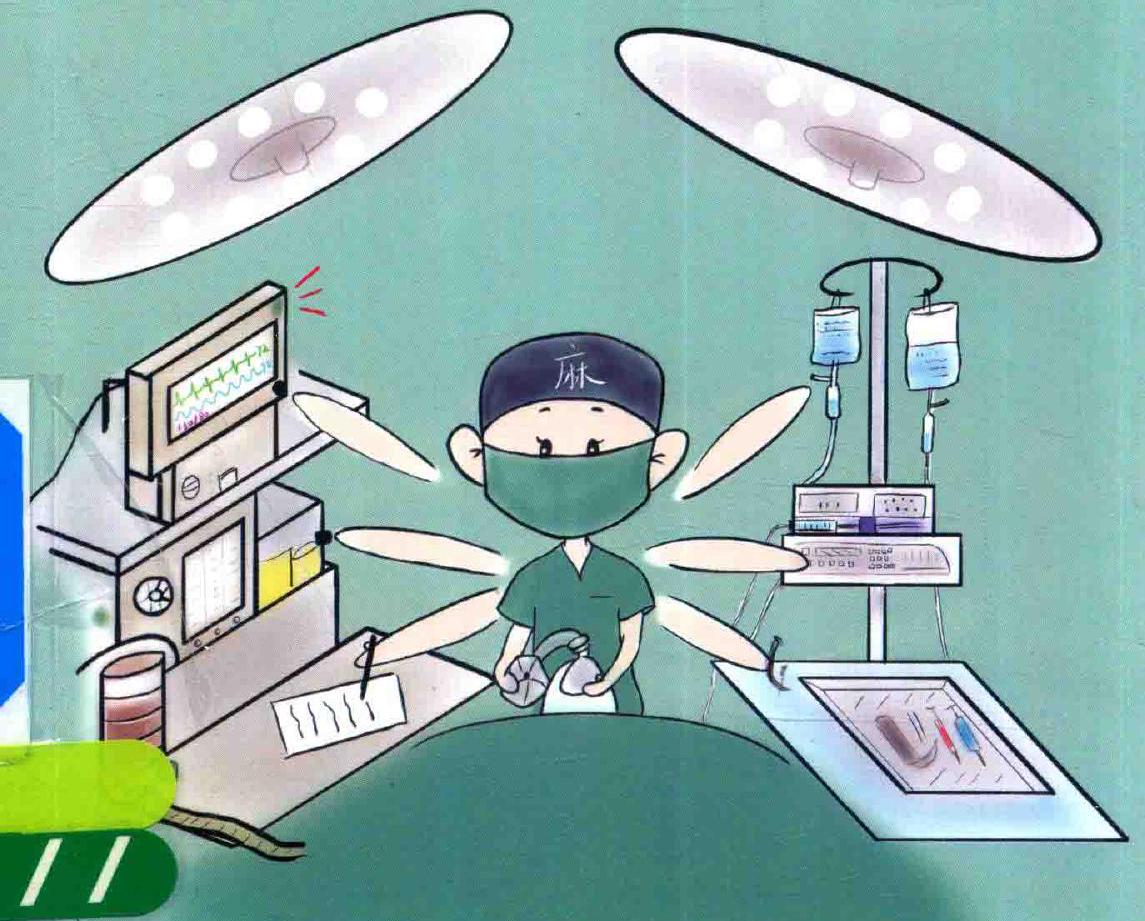
\includegraphics[max width=\textwidth]{2024_07_05_645bb794a4d4f32ee0c8g-001}
\end{center}

北京大学医学出版社\\
责任编辑: 王智敏 袁帅军

封面设计: 方 㵀

封底设计: 孟园园

\begin{center}

\includegraphics[max width=\textwidth]{2024_07_05_645bb794a4d4f32ee0c8g-002}
\end{center}

\begin{itemize}
  \item 国内首部原创麻醉科住院医师手册。
  \item 内容精炼, 有利于麻醉科住院医师、见习实习医师以及基层麻醉医师更好地掌握麻醉学核心知识。
  \item 重点内容以清单 (Checklist)、小贴士(Tips)的形式突出,配以大量表格,方便您学习、记忆和备考。
  \item 双色印刷及画风简洁、轻松的配图和装帧设计,提升您的阅读体验。
\end{itemize}

\begin{center}

\includegraphics[max width=\textwidth]{2024_07_05_645bb794a4d4f32ee0c8g-002(1)}
\end{center}

关注北医社麻醉图书微信公众号

\texttt{https://cdn.mathpix.com/cropped/2024_07_05_645bb794a4d4f32ee0c8g-002.jpg?height=432&width=464&top_left_y=1358&top_left_x=697}\\
获取更多精品图书信息

定价: 55.00 元\\
麻醉科住院医师手册

Handbook for Anesthesia Residents

主编鞠辉冯艺

\section*{MAZUIKE ZHUYUANYISHI SHOUCE}
\section*{图书在版编目(CIP)数据}
麻醉科住院医师手册 / 鞠辉, 冯艺主编. 一北京:北京大学医学出版社, 2017.8

ISBN 978-7-5659-1556-7

I . (1)麻… II . (1)鞠… (2)冯 III . (1)麻醉学 - 手册

IV . (1) R614-62

中国版本图书馆 CIP 数据核字(2017)第 024842 号

麻醉科住院医师手册

主 编: 鞠 辉 冯 艺

出版发行: 北京大学医学出版社

地址: (100191) 北京市海淀区学院路 38 号 北京大学医学部院内

电话: 发行部 010-82802230; 图书邮购 010-82802495

网 址: http: \href{//www.pumpress.com.cn}{//www.pumpress.com.cn}

E-mail : \href{mailto:booksale@bjmu.edu.cn}{booksale@bjmu.edu.cn}

印刷: 北京佳信达欣艺术印刷有限公司

经 销: 新华书店

责任编辑: 王智敏 袁师军 责任校对:金軕文 责任印制:李啸

开 本: $889 \mathrm{~mm} \times 1194 \mathrm{~mm} \quad 1 / 32$ 印张: 11.75 字数: 283 千字

版 次: 2017 年 8 月第 1 版 2017 年 8 月第 1 次印刷

书 号: ISBN 978-7-5659-1556-7

定 价: 55.00 元

版权所有, 违者必究

(凡属质量问题请与本社发行部联系退换)\\
有书由

北京大学医学科学出版基金资助出版

\section*{编者名单}
主编鞠辉冯艺

编 者 (按姓名汉语拼音排序)

段怡冯艺海艇姜柏林

鞠辉潘芳乔青孙亮

田雪伍源张冉 ${ }^{1}$ 张冉 $^{2}$

编写助理 杨丽娜 果 旭 张希峣

插图及封底绘画 孟园园

封面设计 方 璇

注: 本书有两位编者重名, 均为张冓。

\begin{enumerate}
  \item 此编者编写第 3 章第 7 节。

  \item 此编者编写第 3 章第 11 节。

\end{enumerate}

\section*{序}
首先祝贺打开这本手册的年轻住院医师们选择麻醉医学专业一一个既古老又年轻, 而且未来有无限发展空间的临床医学专业。麻醉医学的未来发展方向是围术期医学, 故而, 你们在努力成为一名合格的临床麻醉医师的同时, 还应为成长为优秀的围术期医学医师打下良好基础。你们不仅需要娴熟各项操作技术, 更需要系统掌握内外妇儿的全科基础知识以及具备高超的危机处理能力。优秀源于习惯。也如叶圣陶老先生所言, 我们教育的目的, 也在于学生良好习惯的养成。良好的习惯, 是你们将来成长为优秀麻醉医学医师和围术期医学医师的基础所在。所以住院医师的培养, 也应着力于规范科学思维和工作习惯的培养。

顺应现代麻醉医学的发展趋势, 更注重麻醉医学基本功的培训, 北京大学人民医院的麻醉医师呕心㑂血, 殚精竭虑, 编写了这本培训手册。书中介绍了临床麻醉的基本原则、基础知识和规范流程。内容精炼、重点突出、版面设计新颖、可读性强, 特别是每种操作技能后的清单和小贴士,能够帮助住院医师们养成良好的工作习惯。众多表格和原创的插图, 概述重要知识点, 使本书更易阅读。这是一本值得你们随身携带的口袋书, 它将成为你们成长过程中的良师益友。

\section*{s}
\begin{center}

\includegraphics[max width=\textwidth]{2024_07_05_645bb794a4d4f32ee0c8g-008}
\end{center}

麻醉可确保患者在无痛条件下接受手术, 麻醉医师是手术安全的保护神。古有华佗的 “麻沸散” 用以减轻患者的痛觉, 现代麻醉学更是成为外科手术迅猛发展的三大基础之一。世界首例于新闻报道中公开施行乙醚麻醉的美国医师莫顿的墓碑上写着: “在他以前, 手术是一种极大的痛苦; 从他以后, 科学战胜了疼痛”。不仅如此, 麻醉医师的工作还涉及术前准备和术后处理、危重患者的监护治疗、急救复苏、疼痛治疗等。手术室、病房、急诊室、门诊、内镜室等到处活跃着麻醉医师的身影。用 “起得早, 睡得晚”来形容他们的工作状况不为过一他们是患者进人手术室见到的第一位医师,也是患者术后醒来见到的第一位医师; 他们是 “幕后英雄”一一用自己精淇的专业技术和爱心默默地保障着手术的顺利和患者的安全。他们的工作处处体现着 “有时是治愈, 常常是帮助, 总是去安壂”的医者情怀。

作为北京大学医学部(北医)的附属医院, 承载着传承北大医学的重任, 承担着对年轻医者的培养。北京大学人民医院麻醉科的专家教授们将自己的专业知识、临床经验以及多年来培养住院医师的体会整理编撰成这本《麻醉科住院医师手册》。全书以岗位胜任为导向, 从麻醉科住院医师培养计划开始, 以临床麻醉为主线, 全面系统地介绍了麻醉科住院医师需要掌握的基础理论、基础知识和基本技能。内容详实、图文并茂, 很多插图是医师们的手绘图, 具有很强的实用性。其适用范围已远远超出北京大学人民医院的麻醉科住\\
院医师, 可成为麻醉学科的年轻医师和临床医学专业学位研究生临床学习的重要参考书目。

住院医师培训是医学院校毕业生成长为合格医师的必经之路, 对于提高医疗质量极为重要。北医在百年的医学教育发展进程中, 逐渐建立了规范的住院医师培训体系, 培养了大批优秀的临床医师。培养过程中, 北医的临床医学专家和医学教育管理人员为保证住院医师的培养质量进行了不解的努力, 积累了宝贵的经验。他们无私奉献、默默耕耘, 一代又一代地传承着北医的“厚道”精神。感谢北京大学人民医院麻醉科的老师们!衷心希望年轻的住院医师们能够很好地利用本书,不负老师们的期望,早日成长为一名优秀的麻醉科医师。

段丽萍

北京大学医学部副主任

2017 年 5 月 30 日于北京

\section*{前 言}
北京大学人民医院是北京大学医学部主要教学医院之一, 也是第一批住院医师规范化培训基地之一, 近 20 年已经培养了上百名麻醉科住院医师, 具有丰富的住院医师培养经验。在培养麻醉科住院医师的过程中, 理论知识的学习是必不可少的。我们在住院医师人科时, 即赠送几本经典麻醉学教科书, 方便学生自学以及查阅。然而, 这些年来即使各种麻醉学经典书籍层出不穷, 我们也尚未发现适合住院医师随身携带的麻醉科住院医师手册。目前市场上所售的大量麻醉学经典丛书, 要么太重太厚, 不便于携带; 要么知识极其丰富, 信息量太大,不容易突出住院医师应该掌握的重点; 要么翻译自国外麻醉学手册, 有不少内容不符合我国国情。

在洞悉这种不足以后,北京大学人民医院麻醉科自 5 年前开始编写科内资料《麻醉科住院医师手册》并打印成册,供科内住院医师使用。在不断完善这本资料的同时,我们想到将其出版成书, 以方便更多的麻醉科住院医师学习。感谢北京大学医学科学出版基金的资助, 这大大地推动了本书的进程。

本书由有丰富临床及教学经验的北京大学人民医院麻醉科医师群策群力完成, 参考了国内外多部麻醉学经典著作、指南等文献,对麻醉医师应该掌握的理论知识进行梳理。本书的一个特点是在重要章节中采用清单 (Checklist)的模式提出学习重点内容, 用小贴上(Tips)版块再次重复知识要点, 方便读者总结与记忆。本书是针对住院医师的学习过程\\
进行撰写,适合广大麻醉科住院医师、见习实习医师以及基层麻醉医师阅读。本书还为众多知识点配备了画风轻松的插图以及方便理解的表格, 希望带给工作繁忙的住院医师们一缕清新。本书的第一章, 北京大学人民医院麻醉科住院医师培养总则, 是在国家以及北京市住院医师培训方案和细则的基础上,结合北京大学人民医院自身的教学特点, 经多年来不断实践与完善而成, 供全国各地的麻醉科住院医师以及教学负责人参考借鉴。

这里也要指出, 本书是为麻醉学初学者准备的㪣门砖,麻醉之精深博大不能全部在这里体现。欢迎广大读者给我们提出意见和建议,以便未来再版更上一层楼。衷心希望这本《麻醉科住院医师手册》能对各位麻醉医师的临床工作有所帮助!

鞠 辉 冯艺

\section*{目 录}
第 1 章北京大学人民医院麻醉科住院医师培养\\
总则 ..... 1\\
第一节 麻醉科住院医师培养计划\\
第二节 麻醉科住院医师工作职责与常规 ..... 3\\
第三节 麻醉科住院医师工作常规 ..... 5\\
第 2 章 术前管理 ..... 13\\
第一节 术前访视 ..... 13\\
第二节 术前患者全身状态的评价 ..... 16\\
第三节 麻醉计划的制订 ..... 40\\
第四节 麻醉相关说明及知情同意书 ..... 43\\
第五节 麻醉科术前医嘱(输液、术前药) ..... 45\\
第六节 病例汇报 ..... 50\\
第3章 术中管理 ..... 53\\
第一节 麻醉准备 ..... 53\\
第二节 三方核查 ..... 66\\
第三节 全身麻醉的诱导、维持和苏醒 ..... 67\\
第四节 监护性麻醉 ..... 76\\
第五节 麻醉监测 ..... 78\\
第六节 手术体位 ..... 95\\
第七节 液体治疗 ..... 101\\
第八节 出血与输血 ..... 121

\section*{目 录}
第九节 麻醉期间常见问题的处理 ..... 132\\
第十节 合并症患者的围术期管理 ..... 160\\
第十一节 各种手术的麻醉 ..... 184\\
第 4 章 术后管理 ..... 247\\
第一节 患者手术后去向定夺及转运 ..... 247\\
第二节 气管拔管及离室指征 ..... 249\\
第三节 麻醉恢复室常见并发症及随访要点 ..... 254\\
第四节 术后疼痛管理 ..... 259\\
第 5 章 麻醉操作 ..... 268\\
第一节 面罩通气 ..... 268\\
第二节 气管插管 ..... 273\\
第三菏 喉罩通气 ..... 278\\
第四节 动脉穿刺置管 ..... 282\\
第五节 中心静脉穿刺置管 ..... 287\\
第六节 椎管内麻醉 ..... 293\\
第七节 上、下肢神经阻滞 ..... 302\\
第 6 章 麻醉相关药物 ..... 311\\
第一节 非巴比妥类静脉麻醉药 ..... 311\\
第二节 常用镇静药 ..... 314\\
第三节 阿片受体激动药与怙抗药 ..... 315\\
第四节 吸人麻醉药 ..... 319\\
第五节 肌肉松驰药 ..... 322\\
第六节 局部麻醉药 ..... 325\\
第七节 肾上腺素受体激动药 ..... 325\\
第八节 肾上腺素受体阻滞药 ..... 329\\
第九节 抗胆碱药(选择性抗毒曹碱药) ..... 329\\
第十节 抗胆碱酯酶药 ..... 332\\
第十一节 钙通道阻滞药 ..... 333\\
第十二节 扩血管药物 ..... 333\\
第十三节 抗心律失常药物 ..... 336\\
第十四节 非甾体抗炎药 ..... 336\\
第十五节 止吐药 ..... 342\\
第十六节 糖皮质激素 ..... 342\\
麻醉学常用英汉专业词汇对照表 ..... 345

\begin{center}

\includegraphics[max width=\textwidth]{2024_07_05_645bb794a4d4f32ee0c8g-015}
\end{center}

\section*{北京大学人民医院麻醉科住院智师培养总则}
\section*{第一节 麻醉科住院医师培养计划}
一、培养目标

\begin{enumerate}
  \item 知识面广而深 掌握麻醉学、疼痛医学及危重病医学的相关基础理论知识, 对学科进展有一定的了解。

  \item 熟练的临床技能 熟练掌握麻醉常用技术、技能,掌握现代急救复苏与监测技术, 熟悉新的麻醉方法与技术。

  \item 具备一定的独立工作能力 有较强应变能力。能独立完成常见手术的麻醉。在上级医师的指导下, 能在危重患者的麻醉管理中发挥重要作用。具备一定的教学和科研能力。

  \item 成为 “一专多能”的人才 有倾向性地发展从事专科麻醉, 熟练掌握特殊专业技术, 参与重症监护治疗病房 (ICU)的管理和急救、复苏工作,以及院内会诊。

\end{enumerate}

\section*{二、培养时间}
六年, 其中包括:

\begin{enumerate}
  \item 麻醉住院医师规范化培训,简称 “规培”,为期三年。

  \item 通过规培结业考试者, 进人麻醉专科医师培训, 时间为三年。其中前两年为外科综合麻醉培训, 同既往二阶段

\end{enumerate}

\section*{麻醉科住院医师手册}
住院医师培训。包括不少于半年的总住院医师训练。

专科医师第三年可以选择参加一种麻醉亚专业专科医师培训, 包括心胸血管麻醉、儿科麻醉、产科麻醉、高级外科综合麻醉等。

\section*{三、培养程序}
\begin{enumerate}
  \item 第一年 临床麻醉基础知识及技能的培养。

  \item 第二年 相关学科的培养一心内科, 呼吸内科及 ICU 转科学习。

  \item 第三年 临床麻醉的重点培养, 即从事专科麻醉、危重急症和特殊病种的麻醉工作,掌握专科麻醉技术,培养独立工作能力,提高管理水平。

  \item 第四年 总住院医师的培养, 即给予总住院医师工.作,培养管理能力,提高麻醉水平,成为科内技术骨干,进而成为低年资住院医师的指导医师。

  \item 第五年 科研、教学工作能力的培养, 即参加科内科研与教学工作,承担课题和撰写论文、综述等,承担本科医学生的授课任务。

  \item 第六年 选择性参加麻醉亚专业专科医师培训, 包括心胸血管麻醉、儿科麻醉、产科麻醉、高级外科综合麻醉等。

\end{enumerate}

\section*{四、培养要求}
原则择优培养与使用, 任人唯贤; 德才兼备, 全面发展, 具有较强实力。

\begin{enumerate}
  \item 住院医师培养根据临床工作量、参加理论授课和技能 workshop 培训、理论及操作考核、综合素质评估、参与科研工作等方面进行量化培养与考核。

  \item 具有高尚的医德医风和良好的素质与修养, 有高度

\end{enumerate}

\section*{1 $\cdot$北京大学人民医院麻醉科住院医师培养总则}
的事业心和责任感,勤奋、进取、刻苦实干。

\begin{enumerate}
  \setcounter{enumi}{2}
  \item 为学科的发展积极努力工作, 刻苦学习, 钻研技术,积极参加政治学习、科内活动与业务学习。

  \item 完成论文或综述 $1 \sim 2$ 篇以及译文数篇, 参加临床、实验室及教学工作。

  \item 实行培养后业务考试制度以及医德医风与服务态度考核制度, 每半年一次。合格者, 5 年后推荐晋升为主治医师。

  \item 住院医师由一名主治医师以上职称的医师负责指导。每年总结一次成绩, 找出差距, 改进培养计划。

  \item 搞好科内团结, 与其他科室友好合作, 真诚配合。

  \item 对于总住院医师, 按总住院医师职责条例执行。

\end{enumerate}

\section*{第二节 麻醉科住院医师工作职责与常规}
一、住院医师工作职责

\begin{enumerate}
  \item 住院医师必须具有职业医师资质, 才能参与日常医疗活动。在麻醉科主任领导和主治医师指导下, 参加本科室日常麻醉工作以及教学和科研的具体工作。

  \item 在主治医师指导下, 进行麻醉前访视患者, 参加术前讨论, 与麻醉主治医师共同确定麻醉方法和麻醉前用药,做好麻醉前药品和器材的准备。

  \item 在主治医师的具体指导下, 参加临床麻醉工作, 麻醉期间密切观察病情, 检查输血、输液以及用药情况, 认真填写麻醉记录单。如出现异常变化, 及时与术者联系, 共同研究, 妥善处理, 并报告上级医师。

  \item 手术后, 护送患者到麻醉恢复室、病房或 ICU, 向护士交代病情以及术后注意事项,并填写 “麻醉病程日志”。

  \item 术后进行随访,将有关情况记人 “麻醉病程日志”。

\end{enumerate}

\section*{麻醉科住院医师手册}
\begin{enumerate}
  \setcounter{enumi}{5}
  \item 严格执行各项规章制度和技术操作规程, 严防差错事故发生。
\end{enumerate}

\section*{二、总住院医师工作职责}
\begin{enumerate}
  \item 本科生医师在第四年或第五年培养期可以担任总住院医师。

  \item 在科主任的领导下, 协助科主任做好科内各项业务与日常医疗管理工作。

  \item 认真检查和督促各项麻醉常规制度和技术操作规程的实施,严防差错事故的发生。

  \item 负责组织和参加科内疑难危重患者的会诊、抢救和麻醉工作。

  \item 每日早晨组织科内的麻醉前病例讨论, 并听取科主任指导性意见。

  \item 协助科主任加强对住院医师、进修医师和实习医师的培训和日常管理工作。

  \item 负责督促每周麻醉记录单的检查与小结工作, 并负责院内会诊登记、医疗差错事故的讨论,以及组织每月一次的麻醉病例讨论。

  \item 协助科主任组织临床质量管理总结会议,督促临床质量改进。

\end{enumerate}

\section*{三、麻醉医师外出气管内插管的管理制度}
\begin{enumerate}
  \item 接到请求会诊通知后, 首先应了解病情, 以便区别对待,例如:患者是成人或小儿,清醒或昏迷,有无困难气道等。

  \item 及时填写会诊插管记录及收费。

  \item 及时填补插管箱内耗材。

  \item 抢救一般患者时,插管前应换刷手衣 $\rightarrow$ 戴手术帽、

\end{enumerate}

\section*{1.北京大学人民医院麻醉科住院医师培养总则}
口罩、护目镜 $\rightarrow$ 戴手套 $\rightarrow$ 穿外出衣; 插管时,应佩戴防溅屏。完成插管回手术室后,先脱鞋套、手套和外出衣。

\begin{enumerate}
  \setcounter{enumi}{4}
  \item 对于发热者或疑似 SARS 患者, 在急诊室插管时,应换刷手衣 $\rightarrow$ 穿隔离衣,戴手术帽(双层)、口罩(双层)、护目镜,穿鞋套,戴手套(双层) $\rightarrow$ 穿防护服。气管内插管时, 应佩戴防测屏。离开急诊室时, 先摘外层手套, 再脱下防护服、外层帽子、口罩、鞋套、摘下护目镜后, 再返回手术室。以上用过的物品均由急诊室负责处理。

  \item 返回手术室后, 先摘手套, 再脱下隔离衣、帽子和口罩,最后洗手、洗澡、更衣。

\end{enumerate}

\section*{第三节麻醉科住院医师工作常规}
\section*{一、麻醉前访视及知情同意制度}
在无特殊原因的情况下,应由主管麻醉医师随访术前患者。通过术前访视, 了解患者的全身状况、并存疾病和严重程度以及治疗情况, 并对治疗结果做出评估; 了解外科疾病对机体生理状态的影响、外科手术类型, 预计术中出血量和 (或)液体转移量,以及评估外科手术本身对循环、呼吸及其他系统的影响; 向患者交代准备选择的麻醉方式, 麻醉和监测可能引起的风险和麻醉并发症及意外, 对患者进行麻醉咨询前宣教, 让患者签署麻醉知情同意书, 并在病程记录单上记录。

对由于严重术前并存疾病没有得到治疗或治疗结果不满意, 而这些疾病可能由此增加麻醉风险的情况,应该同外科医师进行交流,和主刀医生协商,在权衡外科疾病的紧急程度和患者所承受的风险大小之后,决定最佳手术时机,做出对患者更有益的决定。\\
对于有麻醉要求的患者,在麻醉前一天,应让每一位患者阅读、理解并签署《麻醉知情同意书》。《麻醉知情同意书》应该由患者本人或被授权人签字。文盲、无签字能力的患者和不足法定年龄的患者可委托亲属签字。《麻醉知情同意书》在由患者(或被授权人)和麻醉医师共同签字后,才能视为有效。拒绝在《麻醉知情同意书》上签字的患者(或被授权人),麻醉医师有权拒绝给了患者麻醉;对由于拒绝签字而未能及时手术所带来的一切后果,应该由患方负全部责任。《麻醉知情同意书》应该作为患者医疗档案与病历一同保存。麻醉医师根据《麻醉知情同意书》上的规定给予麻醉处理。

住院医师与患者和(或)家属谈话时, 要学会讲究沟通。首先, 介绍自己是患者手术的麻醉医师, 除自己外, 负责此患者麻醉的还有高年资麻醉医师。讨论疾病时,应显示出对患者病情很了解。在介绍麻醉方式、风险、并发症及意外时,既能让患者和(或)家属意识到做手术必须从麻醉中受益,同时又能让其认识到其必须承担的麻醉风险。但让患者和(或家属)明白并发症、意外等发生有一定的概率,并不是每位患者都会发生。让患者体会到做手术有风险,但也是相对安全的。对于美国麻醉医师协会(ASA)分级二级以上或危重患者, 须让家属在《麻醉知情同意书》上签字, 充分说明麻醉风险, 并讲明麻醉医师会做各种努力尽可能地预防和处理麻醉风险。麻醉医师应清楚麻醉前与患者和(或)家属谈话时,什么是必须说的(如风险告知),什么是应该说的(如我们会尽力工作), 什么是不能说的(如过分夸大危险、贬低外科医师等)。

\section*{二、手术安全核查制度( “三方核查”)}
\begin{enumerate}
  \item 手术安全核查由具有执业资质的手术医师、麻醉医师和手术室护士三方共同执行, 分别在麻醉实施前、手术开\\
始前和患者离开手术室前, 对患者身份和手术部位等内容进行核查。手术患者均应佩戴有患者身份识别信息的标识,以便核查。手术医师、麻醉医师和手术室护士分项填写《手术安全核查表》, 并共同确认。无麻醉医师参加的手术, 由手术医师和手术室护士填写相应内容。

  \item 实施手术安全核查的内容及流程

\end{enumerate}

(1)麻醉实施前:核查各方依次确认《手术安全核查表》第一项麻醉实施前的内容:患者身份(姓名、性别、年龄和病案号) 、手术方式、知情同意书、手术部位与标识、麻醉设备安全检查是否完成、植人物、假体、患者过敏史、抗菌药物皮试结果、感染性疾病笁查结果、术前备血情况、皮肤是否完整、术野皮肤准备、静脉通路建立完成、影像学资料等。

(2)手术开始前:核查各方共同核查《手术安全核查表》第二项手术开始前的内容:患者身份(姓名、性别和年龄)、手术方式、手术部位、手术体位、手术及麻醉风险预警(预计手术时间、预计失血量、手术关注点、麻醉关注点、物品灭菌是否合格等),以及切皮前 30 分钟是否给了抗生素等。

(3)患者离开手术室前:核查各方共同核查《手术安全核查表》第三项患者离开手术室前的内容:患者身份(姓名、性别和年龄) 、实际手术方式、手术用药及输血、清点手术用物、确认手术标本,检查皮肤完整性、动静脉通路、引流管、尿管、术后镇痛泵、确认患者去向等。

(4)核查各方填写相关核查项目并在《手术安全核查表》上签字,将此表归人病历中保存。

(5)手术安全核查必须按照上述步骤依次进行,每一步核查无误后方可进行下一步操作,不得提前填写表格。

\begin{enumerate}
  \setcounter{enumi}{2}
  \item 手术科室、麻醉科与手术室负责人是本科室实施手术安全核查制度与持续改进管理工作的主要责任人。\\
麻醉科住院医师手册
\end{enumerate}

\section*{三、麻醉期间对患者的观察、监测和记录制度}
\section*{(一) 观察}
\begin{enumerate}
  \item 只要是需要专职麻醉医师施行的麻醉, 都必须有专职人员在现场观察,不得擅离职守。每位患者必须由一名住院医师(或同等级别)及一位主治或主治以上级别医师共同负责。

  \item 麻醉期间观察的主要任务是观察患者的生命体征,结合必要的监测措施, 及时发现和积极处理麻醉期间出现的异常变化,确保手术患者的生命安全。

  \item 对于保持自主呼吸的患者, 观察患者的呼吸运动类型(胸式或腹式呼吸)、呼吸幅度及频率,口唇黏膜、皮肤及手术野血液的颜色, 以初步判断是否存在呼吸道梗阻、缺氧或二氧化碳蓄积。为全身麻醉(简称全麻)患者在气管内插管或插人喉罩后,应听患者双侧肺呼吸音,以确定导管的位置是否正确。

\end{enumerate}

\section*{(二) 监测}
监测是指采用特殊仪器或设备来测定患者的某些生理参数。应根据病情需要、手术及其风险性的大小和具体条件,选择适当的监测方法。

\begin{enumerate}
  \item 常规监测项目为: 血压(无创性)、心电图(心律、心率)、呼吸频率、尿量、体温和脉搏氧饱和度 $\left(\mathrm{SpO}_{2}\right)$ 。

  \item 对于病情较重或手术较大的患者, 除监测上述参数外, 可选择监测直接动脉压、中心静脉压(CVP)。

  \item 对于危重患者或手术风险性大的患者,除监测上述参数外, 还可选择监测肺动脉压(PAP)、肺毛细血管楔压 (PCWP) 和心排血量(CO), 并计算血流动力学参数。

  \item 对于全麻患者, 应监测潮气量和呼吸频率, 每分通气量(MV)或呼气末 $\mathrm{CO}_{2}$ 浓度 $\left(\mathrm{EtCO}_{2}\right)$, 以保证患者的通\\
气功能正常。设置气道压和通气量的报警界限, 以便发现呼吸环路的意外脱离事件。

  \item 有条件者可选择监测动脉血气分析、吸人氧浓度 $\left(\mathrm{FiO}_{2}\right) 、 \mathrm{EtCO}_{2}$ 、麻醉气体浓度和肌肉松驰程度监测等参数。

\end{enumerate}

\section*{(三)麻醉相关记录}
\begin{enumerate}
  \item 凡是需要专职麻醉医师施行麻醉者, 都必须由一线医生填写,二线医生签字确认以下医疗文件:术前访视单、知情同意书、手术安全核查表、麻醉记录单、麻醉病程单、术后镇痛单。医保和公费医疗患者需填写自费协议书。

  \item 应逐项填写麻醉记录单, 麻醉事件记录应准确、完整。

  \item 在手术结束后保存电子麻醉记录单并打印,打印的麻醉记录单由主管麻醉医生签字后放人病历。

  \item 麻醉记录单填写的主要内容:

\end{enumerate}

(1)患者姓名、年龄、病历号、身高、体重、ASA 分级、麻醉方式(椎管内麻醉的穿刺部位、方法及阻滞范围,全麻气管内插管的途彺, 导管类型如单腔管、双腔管、喉罩等, 导管型号)、气道评估、术前诊断、术后诊断、拟施手术、已施手术、术者姓名、麻醉医生姓名、巡回及器械护士姓名。

(2)麻醉期间的持续吸人药物及静脉给药的名称及剂量。

(3)监测项目:对于常规手术的患者, 每 $5 \sim 10 \mathrm{~min}$ 描记一次无创血压、心率、呼吸频率、体温、脉搏氧饱和度。

(4)麻醉事件记录(包括患者从进人手术室到离开手术室之间所有的麻醉事件、重要的手术步骤、单次给药的名称及剂量)。

(5)麻醉结束后,填写镇痛方式。对于携带镇痛泵的患者, 应填写术后镇痛随访记录单, 记录术中输液、输血量、

\section*{麻醉科住院医师手册}
失血量、引流液量、尿量及患者的转归等。

\section*{四、手术结束后患者的转运制度}
\begin{enumerate}
  \item 手术结束后由麻醉医生和外科医生协商患者的转归:病房、麻醉后监护病房(PACU)、ICU。

  \item 对于手术后直接转回病房的患者, 应观察患者直至其意识恢复、血流动力学稳定、自主呼吸吸空气时脉搏氧饱和度在 $90 \%$ 以上。在转运患者时, 应由麻醉医生、外科医生和卫生员护送。

  \item 对于手术结束后转人 PACU 观察的患者, 待其病情稳定、符合 PACU 的转出标准(Aldrete 评分)后, 由 PACU 的护士、外科医生及卫生员护送转至普通病房。

  \item 对于危重患者, 应在有效治疗措施(吸氧、人工呼吸、输液、应用血管活性药物等)维持血流动力学和呼吸功能稳定后, 才能将患者转送至 ICU 进一步治疗。在转运途中, 除维持患者在手术期间的有效治疗外, 还应监测心电图、血压和 $\mathrm{SpO}_{2}$, 并准备必要的急救措施。虽然手术和麻醉已结束, 但其对患者的生理影响并未完全消除, 患者的各种保护性反射仍未完全恢复, 潜在的危险性仍然存在。因此,在转运患者时, 麻醉医师或麻醉护士应位于患者的头部附近, 负责观察病情, 以便及时发现和处理紧急情况。

\end{enumerate}

\section*{五、北京大学人民医院术后镇痛的管理制度}
\begin{enumerate}
  \item 在术前访视时, 由麻醉医师向患者交代携带自控镇痛装置的必要性及费用问题,并签署知情同意书。

  \item 主治医师根据患者的一般状况、手术情况及麻醉方式选择最佳的镇痛方式, 配置药液, 设置给药方式、持续输注药物剂量、患者自控镇痛洜 (PCA) 按压间隔时间、单次给药剂量、单位时间输注总量及药液总量。

\end{enumerate}

\section*{1 $\cdot$ 北京大学人民医院麻醉科住院医师培养总则}
\begin{enumerate}
  \setcounter{enumi}{2}
  \item 由主治医师确认镇痛随访记录单内患者的一般资料、镇痛方式、镇痛泵开始时间及镇痛泉的设置, 并签字。

  \item 手术完毕前 30 分钟, 安装自控镇痛装置, 充分排气后与患者端相连接。

  \item 术中特殊情况及需要随访人员重点访视的内容应在镇痛随访记录单中注明。

  \item 麻醉医师护送患者转回病房, 与陪护人员交代自控镇痛装置的使用方法及注意事项,告知患者若出现严重的恶心呕吐、皮肤瘙痒、疼痛强度评分 $\geqslant 4$ 分等不良反应或自控镇痛装置报警时应及时通知护士。护士应将患者的情况或自控镇痛装置报警的相关信息及时反馈给麻醉科医生。

  \item 随访人员每日下载前一日手术患者镇痛随访的相关信息。随访完毕后, 将资料上传回电脑, 以便主治医师能及时了解其患者的镇痛效果。

  \item 随访人员从术后第一天开始对患者进行镇痛随访并填写镇痛随访记录直至患者停止使用自控镇痛装置。

  \item 镇痛随访的内容包括: 患者生命体征的变化, 疼痛强度的评分, 按压次数及剩余药量, 下肢运动情况, 睡眠情况, 有无恶心呕吐、皮肤症㾕、尿渚留、过度镇静、呼吸频率 $\leqslant 8$ 次 / 分钟等不良反应。

  \item 对于采用硬膜外镇痛的患者, 观察硬膜外穿刺点有无渗出及插人深度。若在手术当日或术后第一日硬膜外导管脱出,应更换其他镇痛方式并通知主治医师。

  \item 在停止使用自控镇痛装置治疗后, 应记录患者对术后治疗的总体满意度。

  \item 建立术后镇痛交接记录本, 对需要交班的内容进行记录, 保证疼痛治疗的连续性, 发现问题及时处理。

  \item 若遇患者有严重副作用, 随访人员应先停止使用镇痛装置, 告知主治医师, 必要时通知科室主任, 及时调整镇

\end{enumerate}

\section*{麻醉科住院医师手册}
痛方案,并给予患者及时、正确的诊治。对于镇痛不全及副作用不能耐受的患者, 给予处理后应多次巡视直至患者疼痛强度评分 $\leqslant 3$ 分,副作用可以耐受。

\begin{enumerate}
  \setcounter{enumi}{13}
  \item 自控镇痛装置药袋内的药液含阿片类药物的成分,停止镇痛装置后,应将药袋毁形,剩余药液倾倒。

  \item 一次性术后自控镇痛装置药袋单次使用时间不应超过 96 小时。

  \item 对于在术后应用低分子朋素皮下注射治疗的患者,硬膜外导管的拔出时间应在用药前 4 小时或给了低分子肝素治疗后 12 小时。

\end{enumerate}

\section*{17. 整理术后镇痛随访资料并存档。}
\begin{enumerate}
  \setcounter{enumi}{17}
  \item 麻醉科全体人员应两个月进行 1 次术后镇痛的质量控制,总结经验、修正问题。
\end{enumerate}

\section*{六、麻醉后访视制度}
\begin{enumerate}
  \item 对于手术后由 PACU 转至病房的患者, 麻醉医师应在患者转出PACU 前填写麻醉病程日志及术后随访内容。

  \item 对于其他的手术患者, 在术后 $24 \sim 72$ 小时内进行随访。并将随访结果记人麻醉单或病程日志。

  \item 主治医师(或住院总医师)应随访观察患者。对于有麻醉相关并发症的患者, 需给出诊断和治疗意见。若患者有严重并发症,应向主任汇报。随访主要内容包括:了解麻醉后恢复情况, 有无与麻醉相关的并发症。对于有麻醉并发症的患者,应继续随访,并参加相关的讨论和处理。

\end{enumerate}

(鞠 辉 冯 艺)

\section*{术前管理}
\section*{第一节 术前访视}
一、概述

(一) 术前访视的目的

\begin{enumerate}
  \item 了解患者需行手术治疗的外科疾病及并存的其他系统疾病。

  \item 制订合理可行的麻醉管理方案。

  \item 完善术前检查, 开具术前麻醇医啒。

  \item 减轻患者的焦虑, 建立良好互信的医患关系; 让患者签署麻醉知情同意书。

\end{enumerate}

\section*{(二)术前访视的最终目标}
降低患者围术期并发症的发生率和病死率, 改善其预后。

\section*{二、术前访视的流程}
\section*{(一)第一步: 查看病历}
\begin{enumerate}
  \item 病历记录 重点了解现病史、既往史、体格检查,以及病情变化; 评估患者术前全身状态(详见本章第二节 “术前患者全身状态的评价”)。

  \item 护理记录了解身高、体重、体温、尿量及疼痛评分等, 特别是动态变化。

  \item 实验室检查 了解血常规, 尿常规, 电解质水平,生化, 凝血, 血型及备血, 感染指标 [如乙型肝炎(乙肝)、丙型肝炎(丙肝)、梅毒、人类免疫缺陷病毒(HIV)],血气分析,特殊检查。

  \item 影像学检查 心电图, 胸部 X 线检查, 肺功能检查,超声心动图, 其他超声学检查, 冠状动脉造影检查, 计算机断层扫描术(CT)及磁共振成像(MRI)检查。

  \item 用药医嘱 明确患者人院期间的用药情况, 可以提示患者病情严重程度; 明确药物停用种类及时间。

  \item 会诊记录 明确专科指导意见,综合判断患者病情。

\end{enumerate}

\section*{(二)第二步:问诊和查体}
\section*{1. 问诊}
(1)对象:患者及家属 [注意特殊患者:未成年人, 肿痹患者(隐瞒病情), 智力障碍患者及䶮哑患者(沟通与交流障碍),吸毒者、情绪激动者及有暴力倾向者(注意用词,避免冲突)]。

(2)内容:主要阳性及阴性症状,如是否有心前区疼痛、胸闷喘憋、咳嗽咳痰、夜间打鼾、异常出血等。

\section*{2. 查体}
(1)视诊:判断气管插管难易度、特殊体位、椎管内穿刺条件等。

(2)触诊: 动静脉穿刺条件预估; 心房颤动患者, 需检查心室率等。

(3)听诊:肺部及心脏等。

\section*{(三)第三步:消除患者疑虑,签署知情同意书}
简明抳要地解答患者及家属的疑问, 告知围术期一切可\\
能出现的风险及意外。不要草率了事, 不行表面文章。对于有些重要内容, 若麻醉知情同意书中未予提及, 可以让患者及家属手写补充并签字。

\section*{(四)第四步:与外科医师充分沟通,开具麻醉前医嘱}
对于特殊的患者, 术前应与外科医师充分沟通, 做好充分的术前准备。开具麻醉前医嘱,包括外科医师忽略但需完善的术前实验室检查及麻醉前用药医嘱。

(五)第五步: 访视总结, 制订合理的麻醉方案, 列出麻醉计划

术前访视的流程总结于图 2-1-1。

\begin{center}
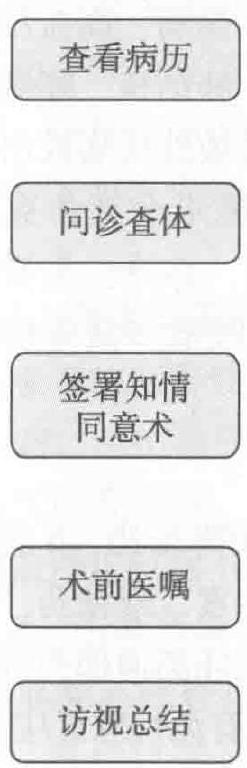
\includegraphics[max width=\textwidth]{2024_07_05_645bb794a4d4f32ee0c8g-029}
\end{center}

\begin{itemize}
  \item 病历记录, 护理记录, 实验室检查, 影像学检查, 用药医嘱等
  \item 向患者及家属确认患者情况
  \item 说明麻醉操作流程以及并发症,解答患者疑问,签署麻醉知情同意书
  \item 术前药物、输液等医殿
  \item 麻醉方案、麻醉计划
\end{itemize}

图 2-1-1 术前访视流程

\section*{第二节 术前患者全身状态的评价}
一、系统性回顾

\section*{(一)本次手术情况}
在麻醉前访视中, 需与手术医师交谈, 了解手术意图,部位、切除脏器范围、手术难易程度、可能出血程度、手术需时长短、手术危险所在, 以及是否需要专门麻醉技术(如低温、控制性低血压等)配合。

\section*{(二)既往史}
特别是与麻醉有关的疾病(如抽㹡、癫㾁、高血压、脑血管意外、心脏病、冠心病、心肌梗死、肺结核、哮喘、慢性支气管炎、肝炎、肾病、脊柱疾病、过敏性疾病或出血性疾病等), 同时追问是否出现过心肺功能不全或休克等症状, 近期状况如何, 特别对心前区疼痛、心悸、头晕、昏厥、活动后呼吸困难、夜间憋醒、长期咳嫩多痰等症状应引起重视。

\section*{(三)治疗用药史}
有些手术患者因治疗需要, 常规应用降压药、 $\beta$ 受体阻滞药、皮质激素、洋地黄、利尿药、抗生素、降糖药、抗癌药、镇静安定药、单胺氧化酶抑制药、三环类抑郁药等, 应了解其药名、用药持续时间和用药剂量,有无特殊反应。

\section*{(四)既往麻醉手术史}
\begin{enumerate}
  \item 既往做过哪种手术, 用过何种麻醉药和麻醉方法,麻醉中及麻醉后是否出现特殊情况, 有无意外、并发症和后遗症, 有无药物过敏史, 家庭成员中是否也发生过类似的麻\\
醉严重问题。

  \item 既往手术可能影响麻醉方案, 例如有既往颈椎固定手术史患者, 其麻醉处理就不同于正常颈椎和呼吸道的患者。又如正在进行动静脉瘘血液透析的患者, 应避免在患肢行动脉和静脉穿刺置管。

  \item 了解既往对某些麻醉药的不良药物反应(如患者既往对琥珀胆碱出现异常肌松延长史, 或有恶性高热病史)。

  \item 重点询问患者在既往麻醉后有无并发症, 若确实存在, 本次麻醉方案就要据此进行改变, 或者预防并发症的发生(如牙齿损伤,术后恶心呕吐)。

\end{enumerate}

\section*{(五)个人史}
个人史包括: 劳动能力, 能否胜任较重的体力劳动和剧烈活动, 劳动或活动后是否出现心慌气短; 有无饮酒、吸烟嗜好,每日饮酒或吸烟量多少,有无长期咳嗽、咳痰、气短史; 有无吸毒成瘾史; 有无长期服用安眠药等历史; 有无怀孕等。

\begin{enumerate}
  \item 吸烟与嗜酒 必须询问每日的摄取数量和持续时间,此类患者的麻醉性药物用量一般需增加。吸烟可产生诸多不利影响, 包括黏膜分泌与清除能力减弱、小气道口径缩小,免疫反应改变等。术前应劝说患者至少停止吸烟 2 个月, 即使术前停止吸烟不到 24 h, 患者也可能获益。

  \item 违禁药应用史 术前应询问是否应用违禁药品, 是否已成㿈。应将这类病例列为高危病例,因其有可能感染 HIV, 需进行鉴别诊断试验。一旦确定患者已有药物成瘾史,围术期都应对戒断综合征采取预防或治疗措施。

  \item 对于已出现戒断综合征的患者, 除非急诊,应延期手术。对于术前因治疗而使用阿片类药物, 或滥用阿片类药物的患者,术中和术后应用阿片类药物时应考虑增加剂量。

  \item 对于运动员患者, 应询问是否应用促蛋白合成丝体类药(合成类固醇药物),因这类药物对肝可产生显著的副作用, 可出现胆汁性黄病。

\end{enumerate}

\section*{(六)过敏史}
\begin{enumerate}
  \item 对患者的过敏反应要足够重视, 但应与药物副作用有所鉴别。例如可待因可引起呕吐(属于副作用)或症痒性皮疹(属于过敏症状),两者都被患者习惯地称为 “过敏”。又如牙科医生使用含肾上腺素的利多卡因施行局部麻醉时, 患者常出现心动过速的副作用, 而患者常会主诉对局部麻醉药过敏。

  \item 青霉素类与头胞菌素类之间的交叉过敏反应率可达 $10 \% \sim 15 \%$ 。如果患者曾有注射青雽素类出现即刻高敏反应史(表现为过敏性休克、血管性水肿和菷麻疹), 那么其对头孢菌素类亦可能过敏, 应换用其他抗生素。如果患者有青䨐素类延迟型过敏反应史, 则可考虑改用头胞菌素类。对碘过敏的患者,应避免使用含碘的药物。

  \item 患者对局麻药的真性过敏反应极为罕见。对麻醉药过敏的患者,在择期手术或神经阻滞麻醉前,可慎重施行皮内过敏试验。

\end{enumerate}

\section*{二、全身状态的评估}
\section*{(一)心血管系统}
\begin{enumerate}
  \item 心功能分级 最常用的方法仍是根据心脏对运动量的耐受程度来衡量。目前常采用纽约心脏病学会(NYHA)四级分类法(表 2-2-1)。\\
表 2-2-1 NYHA 心功能分级及其意义
\end{enumerate}

\begin{center}
\begin{tabular}{|c|c|c|c|}
\hline
心功能分级 & 屏气试验 & 临床表现 & 心功能与耐受力 \\
\hline
I & $30 \mathrm{~s}$ 以上 & \begin{tabular}{l}
体力活动不受限, 无症 \\
状, 日常活动不引起疲 \\
乏, 心悸和呼吸㕅难 \\
\end{tabular} & 心功能正常 \\
\hline
II & $20 \sim 30 \mathrm{~s}$ & \begin{tabular}{l}
能胜任正常活动, 但不 \\
能跑步或较用力地工 \\
作, 否则心慌气短 \\
\end{tabular} & \begin{tabular}{l}
心功能欠佳。麻 \\
醉处理恰当, 麻 \\
醉耐受力仍较好 \\
\end{tabular} \\
\hline
III & $10 \sim 20 \mathrm{~s}$ & \begin{tabular}{l}
体力活动显著受限, 轻 \\
度活动即出现症状, 休 \\
息后尚感舒适 \\
\end{tabular} & \begin{tabular}{l}
心功能不全。麻 \\
醉前准备充分, \\
麻醉中避免增加 \\
任何心脏负担 \\
\end{tabular} \\
\hline
IV & $10 \mathrm{~s}$ 以内 & \begin{tabular}{l}
休息时也出现疲乏、心 \\
悸、呼吸困难或心绞 \\
痛, 任何体力活动均增 \\
加不适感 \\
\end{tabular} & \begin{tabular}{l}
心功能衰晹。麻 \\
醉耐受力极差, \\
手术必须推迟 \\
\end{tabular} \\
\hline
\end{tabular}
\end{center}

\begin{enumerate}
  \setcounter{enumi}{1}
  \item Goldman 心脏危险性指数(表 2-2-2)可为非心脏手术的心脏危险性指数评估(表 2-2-3)提供参考。
\end{enumerate}

表 2-2-2 Goldman 心脏危险性指数 ( cardiac risk index, CRI )

\begin{center}
\begin{tabular}{|c|c|c|}
\hline
评估项目 &  & 分数 \\
\hline
\multirow[t]{2}{*}{病史} & 年龄 $>70$ 岁 & 5 分 \\
\hline
 & 最近 6 个月内发生过心肌梗死 & 10 分 \\
\hline
\multirow[t]{2}{*}{体格检查} & 有主动脉瓣狭窄 & 3 分 \\
\hline
 & 有舒张期奔马律、第三心音或颈静脉充血 & 11 分 \\
\hline
\multirow[t]{2}{*}{$\mathrm{ECG}$} & 有非窦性心律失常 & 7 分 \\
\hline
 & 室性早搏> 5 次 / 分 & 7 分 \\
\hline
一般情况差 & \begin{tabular}{l}
$\mathrm{PaO}_{2}<60 \mathrm{mmHg}(8.0 \mathrm{kPa})$ \\
$\mathrm{PaCO}_{2}>50 \mathrm{mmHg}(6.6 \mathrm{kPa})$ \\
血钾 $<3.0 \mathrm{mmol} / \mathrm{L}$ 或 $\mathrm{HCO}_{3}^{-}<20 \mathrm{mmol} / \mathrm{L}$ \\
\end{tabular} & 3 分 \\
\hline
\end{tabular}
\end{center}

\begin{center}
\begin{tabular}{|c|c|c|c|}
\hline
\multicolumn{3}{|l|}{评估项目} & \multirow{2}{*}{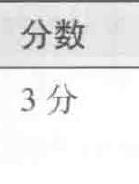
\includegraphics[max width=\textwidth]{2024_07_05_645bb794a4d4f32ee0c8g-034}
} \\
\hline
一般情况差 & \begin{tabular}{l}
BUN $>7.5 \mathrm{mmol} / \mathrm{L}$ \\
ALT 异常, 有慢性 \\
\end{tabular} & \begin{tabular}{l}
$\mathrm{er}>270 \mu \mathrm{mol} / \mathrm{L}$ \\
病 \\
\end{tabular} &  \\
\hline
\multirow[t]{2}{*}{手术种类} & (1)腹腔内、胸腔 & 手术 & 3 分 \\
\hline
 & (2) 急症手术 &  & 4 分 \\
\hline
\multicolumn{4}{|c|}{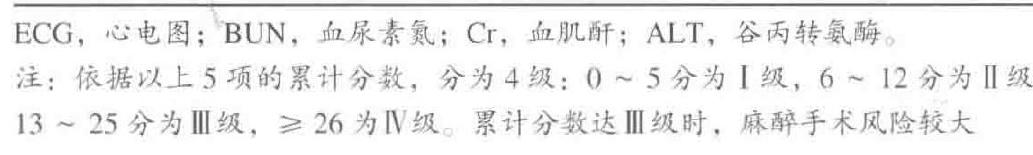
\includegraphics[max width=\textwidth]{2024_07_05_645bb794a4d4f32ee0c8g-034(1)}
} \\
\hline
表 2-2-3\cjkstart根抽( & \multicolumn{3}{|c|}{根据 Goldman 心脏危险性指数进行风险评估} \\
\hline
评分 & 死亡率(\%) & \multicolumn{2}{|c|}{严重心血管并发症发生率(\%)} \\
\hline
$<6$ & 0.2 & \multicolumn{2}{|l|}{0.7} \\
\hline
$6 \sim 25$ & 4 & \multicolumn{2}{|l|}{17} \\
\hline
$>25$ & 56 & \multicolumn{2}{|l|}{22} \\
\hline
\end{tabular}
\end{center}

\begin{enumerate}
  \setcounter{enumi}{2}
  \item 活动耐量的评估 代谢当量(metabolic equivalent, MET)以某种活动所消耗能量是安静时的几倍来表示, 当活动耐量 $<4$ METs 时, 定义为功能储备差(图 2-2-1)。
\end{enumerate}

\begin{verbatim}
1.05\times体重(kg) 
3 METs 普通步行 ( }4\textrm{km}/\textrm{h})\mathrm{ ),低强度的肌肉训练,打排球
4 METs 快走( }6.4\textrm{km}/\textrm{h})\mathrm{ , 打高尔夫, 骑自行车, 打保龄球,
    轻松地爬两层楼
6METs 轻松地慢跑, 有氧运动, 上下楼梯
8METs 跑步,游泳,搬运重物
说明:良好, 7METs以上; 中等, 4 7METs; 低下, 4METs以下
\end{verbatim}

\section*{图 2-2-1 METs 量表}
\section*{4. 心血管疾病患者麻醉耐受力的评估}
(1)高血压:首先明确是原发性高血压还是继发性高血压,警惕是否为未诊断的嗜铬细胞痹。高血压患者的麻醉风险取决于是否继发重要脏器(心、脑、肾)损害及其程度。单纯高血压, 不合并冠状动脉病变、心力衰竭或肾功能减退等,在充分的术前准备和恰当的麻醉处理前提下, 麻醉耐受良好。术前准备的重点是抗高血压治疗。

高血压患者在术中和术后均可能发生高血压、低血压、心力衰竭、心脑血管意外等并发症。合并糖尿病和肥胖者,其麻醉的危险性更大。

高血压患者在术前需经内科治疗, 应用降压药使血压控制在 $160 / 90 \mathrm{mmHg}$ 以下, 改善其他重要脏器功能及水电解质平衡后,方可进行手术麻醉。

急症手术前, 亦应调控好患者的血压及全身状态, 方可施行麻醉。

(2)冠心病: 麻醉危险在于围术期心肌梗死(心梗)发作。麻醉前应该明确:患者是否存在心绞痛及其严重程度;是否发生过心肌梗死,最近发作时间。患者发生心肌梗死后 6 个月内,围术期再梗率高,且预后差,因此择期手术宜在急性心梗发作 6 个月后, 且依据当前患者的心脏功能代偿状况而定。

(3)先天性心脏病

\begin{itemize}
  \item 房间隔缺损或室间隔缺损:心功能为 I、 II 级, 既往无心力衰竭史, 可接受一般手术, 无特殊危险; 若伴有肺动脉高压,死亡率增加,应推迟手术。
  \item 肺动脉瓣狭窄:轻度者, 不是手术禁忌证; 重度者,易发作急性右侧心力衰竭,禁忌择期手术。
  \item 法洛四联症:麻醉后易引起心排血量骤减和严重低氧\\
血症, 择期手术危险性极大。
\end{itemize}

(4)心律失常: 明确引起心律失常的原因和对血流动力学的影响。对于无明显自觉症状、无严重血流动力学改变的单纯性心律失常患者, 不增加麻醉风险, 可不了特殊处理。但以下情况应引起高度重视:

\begin{itemize}
  \item 年龄 $>45$ 岁, 伴有心脑血管疾病或有糖尿病史者。
  \item 心房颤动和心房扑动:术前心室率能控制在 80 次 / 分左右,不增加麻醉危险;心室率>100 次/分或 $<60$次/分,提示有严重心脏病变或其他原因(如甲状腺功能元进),则麻醉危险性显著增加。
  \item 室性期前收缩:偶发者, 多属于功能性, 一般无需特殊处理; 频发(>5 次/分), 或呈二联律、三联律、系多源性或呈 “R on T”, 容易演变为室性心动过速或心室颤动,术前必须给予治疗,择期手术宜推迟。
  \item II 度以上房室传导阻滞或慢性双束支阻滞(右束支伴左前或左后束支传导阻滞), 有发展为完全性心脏传导阻滞而猝死的可能, 术前需做好心脏起搏器准备。
  \item 预激综合征:可发作室上性心动过速, 一般只要做到防止交感神经兴奋和血管活性物质释放即可。但对于症状持续而原因不明者, 应引起重视。这往往是心肌病变的唯一症状, 麻醉危险性极高, 择期手术必须推迟。
  \item 赎性心律失常:须分辨其原因,如为病态窦房结所致,宜做好应用异丙肾上腺素和心脏起搏器的准备。
  \item 无论何种心律失常, 发作时伴有头晕、头痛、黑矇及血流动力学改变, 或与心绞痛发作有关者, 意味着麻醉风险性增加,应做好充分准备。
\end{itemize}

(5)心脏瓣膜病:心脏瓣膜病的麻醉危险性主要取决于病变的性质及其心功能损害的程度, 麻醉前应识别是以狭窄为\\
主, 还是以关闭不全为主, 或者两者兼有。

以狭窄为主者的病变发展较关闭不全者迅速, 重度主动脉㦚狭窄或二尖瓣㹫窄极易并发严重心肌缺血、心律失常 (心房扑动或心房颤动)和左室心力衰竭,也易并发心腔血检形成和栓子脱落, 因而麻醉危险性相当高, 一般应禁忌施行择期非心脏手术。

心脏瓣膜关闭不全者对麻醉和手术耐受力一般尚可,但易继发细菌性心内膜炎或缺血性心肌改变, 因而有猝死可能。

\section*{(二)呼吸系统}
\section*{1. 麻醉前应了解患者有无呼吸系统疾病及其他系统并}
存疾病 若患者处于急性呼吸系统感染期间,如感冒、咽炎、扁桃体炎、气管支气管炎或肺炎, 手术必须推迟到完全治愈 $1 \sim 2$ 周后,否则术后易并发肺不张和肺炎。

临床评估呼吸系统慢性感染和呼吸功能不全的病史和体征有:

(1)呼吸困难: 活动后呼吸困难是衡量肺功能不全的主要临床指标。

(2)慢性支气管炎: 凡一年中有持续 3 个月时间的慢性咳嗽、多痰, 且有两年以上病史者, 可诊断为慢性支气管炎。此为慢性阻塞性肺疾病, 术后易发生肺泡通气不足或肺不张。

(3)感冒: 为病毒性呼吸道感染, 抑制呼吸功能、呼吸道阻力增加, 患者对感染的抵抗力降低。

(4)哮喘: 提示呼吸道已明显阻塞。

(5)吸烟: 每天吸烟 $10 \sim 20$ 支, 即使是青年人, 肺功能也会开始变化; 每天 20 支以上, 并有 10 年以上吸烟史者,通常并存慢性支气管炎。术前戒烟 $24 \sim 48 \mathrm{~h}$, 可降低患者碳氧血红蛋白含量; 术前戒烟超过 4 周, 可改善纤毛功能并减

\section*{麻醉科住院医师手册}
少气道分泌及刺激性。若要择期手术, 至少应要求患者戒烟 2 周, 彻底控制感染, 改善通气功能。

(6)高龄:老年并存慢性疾病, 尤以阻塞性肺疾病和肺实质性病变多见, 可继发引起肺动脉高压和肺源性心脏病(肺心病), 这是老年人麻醉主要危险原因之一, 须做好细致的术前工作。

\section*{2. 简单易行的肺功能估计方法}
(1)测胸腔周径法:测量深吸气与深呼气时胸腔周径的差值。超过 $4 \mathrm{~cm}$ 以上者, 提示无严重的肺部疾病和肺功能不全。

(2)屏气试验:患者安静 5-10 min, 深呼吸数次后, 在深吸气后憋气, 记录屏气时间。屏气时间超过 $30 \mathrm{~s}$ 以上者,提示心肺功能良好; 若屏气时间小于 $20 \mathrm{~s}$, 则提示心肺功能不全。

(3)吹气试验:让患者在尽量深吸气后做最大呼气。若呼气时间小于 $3 \mathrm{~s}$, 提示肺活量基本正常; 若超过 $5 \mathrm{~s}$, 则表示可能有阻塞性通气功能障碍。

(4)吹火柴试验: 患者安静后, 嘱其深吸气, 然后张口快速呼气, 能将 $15 \mathrm{~cm}$ 远的火柴吹熄者, 提示肺储备功能良好,否则肺储备功能低下。

(5)登楼梯运动试验:患者用正常速度不间断登上 3 层楼后, 若患者能在 $10 \mathrm{~min}$ 内心率和呼吸频率完全恢复至登楼前水平,且无心律失常,则表明心、肺功能良好。

\begin{enumerate}
  \setcounter{enumi}{2}
  \item 呼吸困难的评级(表 2-2-4)活动后呼吸困难(气短)是衡量肺功能不全的主要临床指标。\\
表 2-2-4 呼吸困难的评级*
\end{enumerate}

\begin{center}
\begin{tabular}{ll}
0 级 & 平地正常行走无呼吸困难症状 \\
I 级 & 能按需行走, 但易疲劳 \\
II 级 & 行走距离有限, 行走一定距离后需停步休息 \\
III 级 & 短距离行走即出现呼吸困难 \\
IV 级 & 静息时出现呼吸困难 \\
\end{tabular}
\end{center}

*指呼吸系统疾病引起的呼吸困难。根据正常步速、平道步行结束后观察

\begin{enumerate}
  \setcounter{enumi}{3}
  \item 估计手术后并发肺功能不全的高危指标(表 2-2-5)
\end{enumerate}

表 2-2-5 估计手术后并发肺功能不全的高危指标

\begin{center}
\begin{tabular}{lll}
\hline
肺功能测验项目 & 正常值 & 高危性值 \\
\hline
肺活量 (VC) & $2.44 \sim 3.74 \mathrm{~L}$ & $<1.0 \mathrm{~L}$ \\
第 1 秒用力呼气量 $\left(\mathrm{FEV}_{1}\right)$ & $2.83 \mathrm{~L}$ & $<0.5 \mathrm{~L}$ \\
最大呼气流率(MEFR) & $336 \sim 288 \mathrm{~L} / \mathrm{min}$ & $<100 \mathrm{~L} / \mathrm{min}$ \\
最大通气量(MVV) & $82.5 \sim 104 \mathrm{~L} / \mathrm{min}$ & $<50 \mathrm{~L} / \mathrm{min}$ \\
动脉血氧分压 $\left(\mathrm{PaO}_{2}\right)$ & $90 \sim 100 \mathrm{mmHg}$ & $<55 \mathrm{mmHg}$ \\
动脉血 $\mathrm{CO}_{2}$ 分压 $\left(\mathrm{PaCO}_{2}\right)$ & $35 \sim 45 \mathrm{mmHg}$ & $>45 \mathrm{mmHg}$ \\
\hline
\end{tabular}
\end{center}

\section*{5. 呼吸功能及麻醉危险性的评估(表 2-2-6)}
表 2-2-6 呼吸功能及麻醉危险性评估

\begin{center}
\begin{tabular}{|c|c|c|c|c|}
\hline
\begin{tabular}{l}
呼吸功能 \\
损害程度 \\
\end{tabular} & \begin{tabular}{l}
最大通气量 \\
(MVV)(占 \\
预测值 \%) \\
\end{tabular} & \begin{tabular}{l}
残气量/肺 \\
总量 (\%) \\
\end{tabular} & \begin{tabular}{l}
时间肺活量 1 秒率 \\
$\left(\mathrm{FEV}_{1} / \mathrm{FVC}, \%\right.$ ) \\
\end{tabular} & \begin{tabular}{l}
麻醉 \\
危险性 \\
\end{tabular} \\
\hline
正常 & $\geqslant 75$ & $\leqslant 35$ & $\geqslant 70$ &  \\
\hline
轻度 & $60 \sim 74$ & $36 \sim 50$ & $55 \sim 69$ & 轻度 \\
\hline
中度 & $45 \sim 59$ & $51 \sim 65$ & $40 \sim 54$ & 中度 \\
\hline
重度 & $30 \sim 44$ & $66 \sim 80$ & $25 \sim 39$ & 重度 \\
\hline
极度损害 & $\leqslant 29$ & $>80$ & $\leqslant 24$ & 极度 \\
\hline
\end{tabular}
\end{center}

\section*{(三)肝}
\begin{enumerate}
  \item 肝仅占全身体重的 $2 \%$, 但接受的血流量是心排血量的 $20 \%$, 肝动脉供给肝血流的 $25 \%$ 和需氧量的 $50 \%$, 门静脉提供肝血流的 $75 \%$ 和需氧量的 $50 \%$ 。肝疾病的严重程度可通过 Child-Pugh 分级标准来评估(表 2-2-7)。
\end{enumerate}

\section*{表 2-2-7 Child-Pugh 分级}
\begin{center}
\begin{tabular}{llll}
\hline
项目 & \multicolumn{3}{c}{分数} \\
\cline { 2 - 4 }
 & $\mathbf{1}$ & $\mathbf{2}$ & $\mathbf{3}$ \\
\hline
胆红素 $(\mu \mathrm{mol} / \mathrm{L})$ & 34 & $34 \sim 51$ & $>51$ \\
血清白蛋白 $(\mathrm{g} / \mathrm{L})$ & 35 & $28 \sim 35$ & $<28$ \\
腹水 & 元 & 易控制 & 不易控制 \\
凝血酶原时间 $(\mathrm{s})$ & $\leqslant 14$ & $15 \sim 17$ & $\geqslant 18$ \\
朋性脑病 $($ 期 $)$ & 元 & $\mathrm{I} \sim \mathbb{I I}$ & III $\sim \mathrm{IV}$ \\
\hline
\end{tabular}
\end{center}

\begin{enumerate}
  \setcounter{enumi}{1}
  \item 肝功能的临床估计 可采用 Pugh 推荐的肝功能不全的评估分级加以分析(表 2-2-7)。按该表累积计分,1~3 分为轻度肝功能不全; $4 \sim 8$ 分为中度肝功能不全; $9 \sim 12$分为重度肝功能不全。肝病合并出血, 或有出血倾向时, 提示已有多种凝血因子缺乏或不足。若凝血酶原时间(PT)延长、凝血酶时间(TT)延长、部分凝血活酶时间(APTT)显著延长、纤维蛋白原(FIB)和血小板明显减少,提示已出现弥散性血管内凝血(DIC)和纤维蛋白溶解,表示朋已经坏死, 禁忌做任何手术。

  \item 肝病患者的麻醉耐受力估计 急性肝炎患者在术中和术后极易出现凝血机制障碍,除紧急抢救手术外,应禁忌施行任何手术。

\end{enumerate}

慢性肝病患者手术的最大问题之一是凝血机制异常, 术前必须子以纠正。\\
轻度肝功能不全对患者的麻醉和手术耐受力影响不大。中度肝功能不全和濒于失代偿时, 麻醉和手术的耐受力显著减退, 术前需要经过较长时间的严格准备, 方允许择期手术。

重度朋功能不全的危险性极高, 应禁忌施行任何手术。

\section*{(四)肾}
术前必须通过各项检查来判断肾功能, 衡量患者对麻醉和手术的耐受力以便采取各种透析治疗。

\begin{enumerate}
  \item 各类肾病的麻醉耐受力估计 年轻、无肾病史及尿常规正常的患者可认为肾功能良好, 可耐受各种手术和麻醉。老年, 并存高血压、动脉硬化、严重肝病、糖尿病、前列腺肥大等患者, 容易并发肾功能不全, 即使尿常规无特殊异常, 也需做肾功能检查, 以估计其对麻醉和手术的耐受力。
\end{enumerate}

对于慢性肾衰竭或急性肾病患者, 原则上应禁忌施行任何择期手术。近年来,在人工肾透析治疗的前提下,慢性肾衰竭已不再是择期手术的绝对禁忌证, 但其对麻醉和手术的耐受力仍较差。

肾病主要包括肾小球性肾病和肾小管性肾病两类, 此外还有肾结石性肾病。肾小球性病变即肾炎, 可发展为肾病综合征, 患者处于身体总水量过多而血管内血容量减少的状态,发展至末期可出现尿毒症。为减轻水肿, 常使用利尿药治疗,这样血容量可进一步降低。对这类患者术前准备的重点在于调整血容量和水、电解质平衡, 在严密监测下进行补液处理。肾小管一旦发生病变, 机体代谢终末产物在体内潴留, 最终发展为尿毒症。为彻底根治慢性尿毒症, 多数需施行肾移植术,则术前必须通过人工肾或腹膜透析进行充分细致的准备。

患有慢性肾病者, 常易并存其他脏器病变, 需在术前做出正确判断和治疗。常见的并存疾病有:

(1)高血压或动脉硬化: 在肾病所致的低血容量和贫血情况下,易导致心脏做功增高,继发心力衰竭。

(2)心包炎: 严重者可致心脏压塞, 术前用超声波检查可确诊。

(3)贫血:其严重程度一般与尿毒症的程度成正比。对一般择期手术患者,术前应通过输血使血细胞比容升至 $32 \%$以上为宜。对拟施行肾移植术的患者, 为保证移植肾的存活率,有的主张不了输血,有的则主张输血。

(4)凝血机制异常: 尿毒症患者常并存血小板功能异常和 III 因子(组织凝血活酶)活性降低, 术前需施行皮质激素或免疫抑制等治疗。但对于拟施行肾移植术的患者, 则不宜施行免疫抑制治疗。

(5)代谢和内分泌功能紊乱: 包括糖耐量减退、胰岛素拮抗、 IV型三酰甘油过多、甲状旁腺功能元进、自主神经系统功能紊乱、高血钾和酸中毒等, 同时某些药物的排泄和药代动力学也发生改变, 术前应尽可能子以调整, 对麻醉药和肌肉松驰药的选择必须慎重、合理。

在肾结石病例中, $75 \%$ 属草酸钲性质, 术前均需用利尿药和低钻、低盐饮食治疗,因此可出现低血容量问题。为预防患者发生因禁食所致的脱水,术前需静脉补液。

\begin{enumerate}
  \setcounter{enumi}{1}
  \item 肾功能损伤的临床估计 尿液分析(血、糖、蛋白质)、血浆白蛋白、血尿素氮(BUN)、血清肌酐值、内生肌酎清除率、尿浓缩试验和酚红试验等,是临床较有价值的肾功能测定手段。以 $24 \mathrm{~h}$ 内生肌酐清除率和 BUN 为指标, 可将肾功能损伤分为轻、中和重度三类, 详见表 2-2-8。
\end{enumerate}

\section*{(五)内分泌系统}
患有内分泌系统疾病的手术患者, 全身情况变化较突出, 麻醉危险性增加, 应注意围麻醉期处理。内分泌系统功能的评估包括:\\
表 2-2-8 肾功能损伤程度分类

\begin{center}
\begin{tabular}{lllll}
\hline
 & 正常值 & \multicolumn{3}{c}{损伤程度} \\
\cline { 3 - 5 }
 & 轻度 & 中度 & 重度 &  \\
\hline
\begin{tabular}{l}
$24 \mathrm{~h}$ 内生肌 \\
\end{tabular} \{fd5efcee4-5ca1-4e0f-8bf3-03799e73c1f4\} & $51 \sim 80$ & $21 \sim 50$ & $<20$ &  \\
\begin{tabular}{l}
酐清除率 \\
$(\mathrm{ml} / \mathrm{min})$ \\
\end{tabular} &  &  &  &  \\
\begin{tabular}{l}
血尿素氮 \\
$(\mathrm{mmol} / \mathrm{L}) *$ \\
\end{tabular} & $1.79 \sim 7.14$ & $7.5 \sim 14.28$ & $14.64 \sim 25$ & $25.35 \sim 35.7$ \\
\hline
\end{tabular}
\end{center}

*血尿素檳 $\mathrm{mg} / \mathrm{dl} \times 0.357=\mathrm{mmol} / \mathrm{L}$

\begin{enumerate}
  \item 甲状腺病变 甲状腺功能元进者, 应注意心率的控制情况。巨大甲状腺肿需要估计气管是否受压及其程度, 判断是否有气管软化。

  \item 糖尿病了解糖尿病的类型和治疗情况以及目前的血糖水平, 术前血糖应控制在稍高于正常。应注意有无导致其他全身或重要器官和系统的并发症。

  \item 胰岛素瘤 胰岛素瘤瘤体分泌大量胰岛素而引起反复发作性低血糖。麻醉的关键是术中动态监测血糖的变化。

  \item 肾上腺皮质增多症 应注意其所致的糖、蛋白质、脂膅、水、电解质的代谢紊乱以及心血管方面的改变。这类患者对麻醉和手术的耐受力较低。术中应注意防止肾上腺皮质功能不全。对于有显著骨质疏松的患者, 应估计麻醉操作和管理上的困难。

  \item 嗜铬细胞瘤 其病理生理改变是由于儿茶酚胺分泌过多所致。病程长或久未确诊者, 可有儿茶酚胺性心肌炎、营养代谢失调等。麻醉前应估计肿瘤的功能、病情的严重程度、手术难度, 并特别注意术前准备的情况, 重点是控制高血压和改善血容量。传统术前准备包括:术前 2 周使用 $\alpha$ 受体阻滞药(代表药物为酚苄明)控制高血压,以及术前 3 天\\
麻醉科住院医师手册

\end{enumerate}

使用晶体液和胶体液扩容。

\begin{enumerate}
  \setcounter{enumi}{5}
  \item 肾上腺皮质功能不全 包括术前 6 个月以内长期服用糖皮质激素的患者, 一般难以承受较重的手术应激反应,术前应合理使用替代疗法。

  \item 女性患者在月经期间不宜行择期手术, 其凝血功能常低于正常水平。

\end{enumerate}

\section*{(六)中枢神经系统}
\section*{1. 术前神经系统评估的重点内容}
(1)头痛提示可能存在脑瘤或占位病变、颅内高压、脑积水、颅内动脉瘤或脑动静脉畸形。

(2)神志消失(指姐晕和昏厥)提示可能存在心血管系统疾病或癫㾋状态。

(3)弥漫性肌无力提示可能存在神经肌疾病(如肌营养失调、重症肌无力、多发性神经炎)或内分泌(或代谢性)疾病。

(4)单侧性肌无力最常见于脑卒中、短暂性脑缺血发作 (transient ischemic attack,TIA)或脊神经根疾病。

(5)局灶性神经征象提示可能同时并存中枢性与周围性神经疾病, 需进一步行 CT、MRI 检查确诊。

(6)对于新出现的明确而不稳定的征象, 或估计术后有可能发生神经系统功能障碍者,也需进一步深人检查。

\begin{enumerate}
  \setcounter{enumi}{1}
  \item 对于术前已诊断患有神经系统并存疾病的患者, 需具体掌握疾病的持续时间、最近的表现、治疗用药情况、体检和实验室检查结果, 并做最后的诊断。如果最后的诊断结果与以往的诊断不相符时, 需进一步深人研究, 并邀请神经专科医师会诊, 力求全面做好围术期的预防和治疗工作。

  \item 如果拟采用局部麻醉,应对麻醉区的神经功能进行检查并记录。如果麻醉区与手术区系在同一部位, 麻醉科医

\end{enumerate}

\section*{2 ・术前管理}
师则应在麻醉前对可能涉及的部位进行神经功能检查, 并做记录, 特别是对术前已存在的神经系统损伤进行记录, 后者具有重要意义 (因约有 $15 \%$ 麻醉手术后的周围神经损伤患者会针对麻醉科医师提出索赔要求)。

\section*{(七)水和电解质}
判断水和电解质异常, 须根据病因、体征及实验室检查结果等综合分析, 判断其性质是等渗、低渗或高渗性失水,然后采取相应方法进行处理。

\begin{enumerate}
  \item 急诊患者的水、电解质平衡失调中以脱水、低钾或高钾较多见, 其对人体生理功能扰乱也较大, 一般为等渗性脱水, 多伴有血容量不足。血容量的补充以迅速恢复有效循环血量和保持血液携氧能力正常为原则。失血量小于全身血量的 $15 \%$ 时, 可用乳酸钠林格液、血浆代用品等补充, 但输液量须大于失血量的 $2-3$ 倍。急性低钠(即稀释性低钠)可引起脑水肿或脑肿胀, 此时须快速利尿以使血钠水平达 $130 \mathrm{mmol} / \mathrm{L}$, 方可进行麻醉和手术。由慢性疾病所造成的低钠, 常因其非短时间内可以纠正, 同时对麻醉不产生困难,一般可以不做处理。

  \item 低钾时, 心血管的功能难以维持稳定, 若择期手术,应在术前尽早进行补钾, 使血钾达到 $3.5 \mathrm{mmol} / \mathrm{L}$ 以上, 方能进行手术。对急症病例进行麻醉和手术时, 可在心电图监测下, 连续输入含钾溶液, 维持血清 $\mathrm{K}^{+}$浓度, 从而使心血管功能稳定。但须注意, 低钾患者在扩容后, 其尿量恢复到 $40 \mathrm{ml} / \mathrm{h}$ 方可补钾, 且补钾速度不宜超过 $20 \mathrm{mmol} / \mathrm{h}$ 。

  \item 对于高钾患者,有心律失常时,可用 $10 \%$ 葡蒛糖酸钙 $10 \mathrm{ml}$ 静脉推注,或用 $25 \% \sim 50 \%$ 葡萄糖液 $60 \sim 100 \mathrm{ml}$,每 $2 \sim 3 \mathrm{~g}$ 糖加胰岛素 $1 \mathrm{U}$ 静脉推注, 接着静脉滴注 $10 \%$ 葡萄糖液 $500 \mathrm{ml}$, 内加胰岛素 $15 \mathrm{U}$ 。

\end{enumerate}

\section*{(八)四肢、脊柱}
对于拟行椎管内麻醉患者, 应常规检查脊柱和脊髓功能。

\begin{enumerate}
  \item 检查穿刺标志是否清楚。

  \item 明确脊柱有无病变、畸形或变形。

  \item 穿刺点邻近组织有无感染。

  \item 是否存在出血性疾病、出血倾向或正在使用抗凝药治疗。

  \item 是否有经常头痛史。

  \item 是否存在隐性脊髓病变。

\end{enumerate}

如果怀疑上述情况, 为避免发生全脊髓麻醉、脊髓病变加重、椎管内血肿形成、椎管内感染化脓而继发截㿈等严重并发症,应禁用椎管内麻醉。

\begin{enumerate}
  \setcounter{enumi}{6}
  \item 若拟施行桡动脉穿刺置管,施行直接动脉测压,应首先明确桡动脉是否有病变, 然后做 Allen 试验: 术者用双手同时按压患者的桡动脉和尺动脉, 嘱患者反复用力握拳和张开手指 5~7次至手掌变白,松开对尺动脉的压迫,继续保持压迫桡动脉, 观察手掌颜色变化。若手的颜色在 $7 \mathrm{~s}$ 内恢复正常, 表明尺动脉和桡动脉间存在良好的侧支循环, 即 Allen 试验阴性, 可行桡动脉穿刺; 若在 7 $15 \mathrm{~s}$ 颜色恢复,则为可疑阳性, 需进一步检查; 若在 $15 \mathrm{~s}$ 后仍为苍白, 即为 Allen 试验阳性,提示手掌侧支循环不良,不应选择在桡动脉进行穿刺。
\end{enumerate}

\section*{(九)气道}
气道评估包括:一“看”,二“张”,三“仰头”。

\begin{enumerate}
  \item 一 “看”是指从外观上寻找提示可能存在困难气道的体征,包括颈短粗、下颌短小、腭裂,以及颈部肿物、㾝痕、气管移位。

  \item 二 “张”嘱患者张口, 并观察:

\end{enumerate}

(1)牙齿:有无松动、突出,有无义齿。

(2)张口度: 指患者最大张口时上下门齿间的距离, 正常值为 $3.5 \sim 5.6 \mathrm{~cm}$, 能容纳患者示指、中指和无名指 3 根手指。如果能达此标准, 通常表明㑔领关节活动正常; 小于 $3 \mathrm{~cm}$ ,示插管困难;小于 $1.5 \mathrm{~cm}$, 无法用常规喉镜进行插管。

(3)根据 Mallampati(马氏)气道分级进行评估(见图 2-2-2)。咽部结构的气道分级与直接喉镜插管的难易程度密切相关。气道 I 级患者,喉镜显露达 I 级者占 $99 \% \sim 100 \%$;气道 IV 级患者, 喉镜显露多属 III $\sim \mathrm{IV}$ 级; 气道 II 级的患者中有 $10 \%$ 为喉镜显露IV 级。

(4)下领骨活动度: 大多数正常人能将其下牙列移至上牙列之前。临床上行此项检查时, 下牙列可能有以下 3 种最终位置:

a. 位置 A: 下牙列可以突出至上牙列前。

b. 位置 B: 下牙列与上牙列能够闭合, 但不能前移超过上牙列。

c. 位置 C: 下牙列达不到与上牙列的闭合位置。如果患者上牙列前突, 其达到 “位置 A” 极为困难, 常会发生常规喉镜显露声门困难。

\section*{3. 三 “仰头"}
(1)头后仰程度:仰卧位下做最大限度仰颈, 上门齿前端至枕骨粗缝连线与身体纵轴线相交的角度。大于 $90^{\circ}$ 为正常,小于 $80^{\circ}$ 时颈部活动受限,提示可能存在插管困难。

(2)下领间隙:使患者头部在寰枕关节尽量处于伸展, 测量以下几个指标来表示下领间隙的间距, 以此来预测插管的难度:

a. 甲 - 㬵距离, 即甲状软骨切迹至放隆凸的距离。大于 $6.5 \mathrm{~cm}$, 气管插管一般无困难; $6.0 \sim 6.5 \mathrm{~cm}$, 插管可能会有困难; 小于 $6 \mathrm{~cm}$ ,气管插管常很困难。\\
b. 下领骨水平支长度, 即从下领角至㬵突的距离。大于 $9 \mathrm{~cm}$, 气管插管多无困难; 小于 $9 \mathrm{~cm}$, 气管插管操作困难的发生率高。

c. 胸 - 㬵距离, 即从胸骨上窝至颏突的距离。正常大于 $12.5 \mathrm{~cm}$; 如果小于 $12.5 \mathrm{~cm}$, 一般提示气管插管存在困难。

d. 舌 - 㬵问距, 测量时需患者挺直颈部, 头极度前伸并紧闭口腔, 用手指宽度粗略评估喉前下颌骨内面和舌骨之间的空间。正常成人至少应达到两指以上, 否则提示气管插管可能存在困难。

\section*{4. 其他辅助检查气道的方法}
(1) $\mathrm{X}$ 线检查。

(2) 间接喉镜检查。

(3)纤维喉镜检查。

(4)直接喉镜检查(喉镜直视分级, 又称 Cormack 分级,见图 2-2-2)。

(5) 纤维支气管镜检查。

\begin{center}
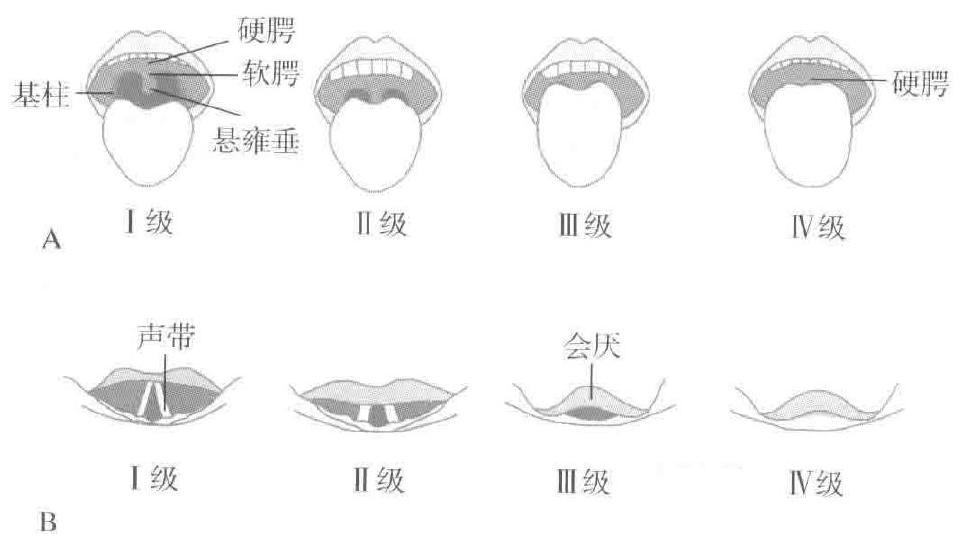
\includegraphics[max width=\textwidth]{2024_07_05_645bb794a4d4f32ee0c8g-048}
\end{center}

图 2-2-2 A, Mallampati 张口度分级; B, 喉镜直视分级

\section*{三、实验室常规检查}
\section*{(一) 心电图}
对于已知有心血管危险因素或需确定危险因素的患者,需进行心电图检查。年龄不能单独作为进行心电图检查的指征。

\begin{enumerate}
  \item 心率异常 对于心动过缓的患者需询问运动时心率是否增快, 必要时可进行阿托品试验或者行 24 小时动态心电图(Holter)检查; 若心动过速, 则需鉴别原因。

  \item 心律异常 偶发期前收缩通常无临床意义; 对于频发患者, 需询问其症状, 并结合心脏基础疾病具体分析。

  \item 传导阻滞 对于 I 度房室传导阻滞、无心动过缓和晕厥等症状且无心脏基础疾病的 II 度房室传导阻滞、单束支传导阻滞的患者, 一般不需要术前安置临时起搏器。相反,合并头晕、黑矇、晕颜症状者, 合并心脏基础疾病者, 合并心动过缓者, 双束支传导阻滞者, 术前应高度重视术中出现高度房室传导阻滞的可能。需要心内电生理专家会诊来评估是否需要术前安置临时起搏器。

  \item 心肌缺血 ST段和 $\mathrm{T}$ 波异常, 提示患者可能存在心肌缺血, 但无确诊意义。病理性 $\mathrm{Q}$ 波提示陈旧性心肌梗死。

  \item 起搏器功能 已经安置永久性起搏器的患者, 术前心电图可以提示起搏器起搏和感知功能是否正常; 已安置植人式心脏复律除颤器(ICD)的患者, 术前需把感知和除颤功能关闭。

\end{enumerate}

\section*{(二)全血检查}
非必需检查。合并以下情况的患者尤其需要关注检查结果:手术的类型及有创性、肝病、高龄、哮喘病史、出血或其他血液系统疾病。

\section*{麻醉科住院医师手册}
\section*{(三)生化检查(如血清钾、血糖、血清钠、肝肾功能}
\section*{检查)}
合并以下情况的患者尤其需要关注生化检查结果:围术期可能的治疗措施、内分泌疾病、肝肾功能障碍发生危险、使用某些药物或替代治疗。高龄患者的实验室检查结果可能与正常值不一致。

\section*{(四)凝血功能检查}
非必需检查。合并以下情况的患者, 尤其需要关注: 出血性疾病、肾功能不全、肝功能障碍、手术的类型及有创性。使用抗凝药物及进行替代治疗可能增加围术期风险。尚无足够的数据用于评估区域麻醉前进行凝血功能检验的可取性。

\section*{(五)麻醉前尿液分析}
除了特殊手术(如泌尿外科手术)或存在泌尿系统症状外,无进行尿液检查的指征。

\section*{(六) 胸部 X 线检查}
非必需检查。合并以下情况的患者, 尤其需要关注胸部 X 线检查: 吸烟、近期上呼吸道感染、慢性阻塞性肺疾病 (COPD) 和心脏病。胸部 X线影像异常在高龄、吸烟、稳定性 COPD、稳定性心脏病、近期上呼吸道感染已治愈患者中的发生率较高, 但并不认为上述因素是应进行胸部 X 线检查的明确指征。

\section*{(七)麻醉前娃娠试验}
患者接受麻醉时, 可能会存在未发现的早期妊娠。现有文献不足以告知患者或临床医师, 麻醉对早期娃娠能否产生有害作用。对于育龄妇女, 可能需要进行妊娠试验, 其试验结果将改变对患者的管理。

\section*{四、特殊检查}
外科手术患者并存明显的内科疾病时, 有必要进行某些特殊检查。

\section*{(一) 心脏疾病}
\begin{enumerate}
  \item 每年约有 700 万 800 万非心脏手术患者并发或死于心脏意外, 其中相当一部分患者的病史中并无冠心病记录。因此,术前确定心脏病这类高危疾病具有重要意义。

  \item 临床上对不能有效控制的充血性心脏病或近 6 个月内有心肌梗死史的患者,建议推迟择期手术。

  \item 当今对已知或怀疑冠状动脉心脏病患者的诊断手段已有显著进展, 如无创的冠状动脉 $\mathrm{CT}$ 检查及有创的冠状动脉造影术。

\end{enumerate}

\section*{(二) 肺功能检查}
\begin{enumerate}
  \item 对于非胸腔手术患者, 术前常规检查肺功能无实际价值,因为预测上腹部手术后的肺部并发症方面,肺功能测定并不比通过仔细询问病史和体检更有效。另外,目前尚无一项肺功能检查异常的项目可以被确认为手术禁忌证。即便患者第 1 秒用力呼气量 $\left(\mathrm{FEV}_{1}\right)$ 低于 $0.45 \mathrm{~L}$, 仍可能耐受手术。

  \item 几项简单的临床资料可以用来预测腹部手术后的肺部并发症,见表 2-2-9。

  \item 对某些需要施行肺切除手术的患者, 则有指征需做更多的检查,如分段肺功能测定、运动试验、右心导管肺动脉压测定等。\\
麻醉科住院医师手册

\end{enumerate}

表 2-2-9 预测腹部手术后肺部并发症的临床资料

ASA 分级大于 2 级

上腹部手术

腹腔内感染

年龄大于 59 岁

肥胖

结肠、直肠、胃、十二指肠手术

心脏手术胸膜腔切开

术前 $\mathrm{PaCO}_{2}$ 高于 $45 \mathrm{mmHg}$

ASA,美国麻醉医师协会

\begin{enumerate}
  \setcounter{enumi}{3}
  \item 动脉血气分析除临床仔细分析病史进行肺功能评估外, 最简单易行的肺功能测定项目是动脉血气分析。如果不存在神经肌肉接头疾病或药物性肺泡通气不足的情况, $\mathrm{PaCO}_{2}$ 大于 $45 \mathrm{mmHg}$ 是预测肺部并发症的可靠指标。
\end{enumerate}

\section*{5. 有创监测}
(1)对于危重择期手术患者, 可提供选定手术有用的参考参数, 判断高危患者病情, 指导纠正血流动力学异常, 从而可降低并发症发生率和死亡率。

(2)对外周血管手术患者进行前瞻性研究指出, 术前施行肺动脉插管监测和纠正血流动力学异常, 术中不良意外(心动过速、心律失常和低血压等)和围术期并发症发生率(主要是吻合血管㭲塞)都比对照组显著减少,但两组的死亡:率、住院天数和住院费用并无显著性差异。

\section*{(三)综合检查与会诊}
对于拟施行复杂大手术, 或常规检查有明显异常, 或并存各种内科疾病的患者, 需做相应的综合性实验室检查, 包括胸部 X 线检查、肺功能测定、心电图、心功能测定、凝血功能检查、动脉血气分析、肝功能检查、肾功能检查、基础代谢率测定及内分泌功能检查等。必要时请专科医师会诊,\\
协助诊断与衡量有关器官功能状态, 商讨术前进一步准备措施。在会诊中, 麻醉医师应提出专门性问题和意见(诸如术中处理、监测、用药和麻醉选择等内容), 避免泛泛提出一些不切实际或过分谦虚的意见。有的医疗中心已建立麻醉科医师术前会诊制度, 由麻醉科医师提出麻醉安危问题。这种会诊方式有助于防止择期手术患者被临时暂停和推迟手术的问题的发生。

\section*{五、麻醉风险评估}
根据麻醉前患者病情和体格情况, 美国麻醉医师协会 (American Society of Anesthesiologists, ASA) 将患者分为六级 (表 2-2-10)。

\section*{表 2-2-10 美国麻醉医师协会(ASA)麻醉分级}
\begin{center}
\begin{tabular}{|c|c|}
\hline
ASA 麻醉分级 & 说明 \\
\hline
ASA I & \begin{tabular}{l}
患者的重要器官功能正常, 体格健壮, 能耐受麻醉 \\
和手术 \\
\end{tabular} \\
\hline
ASA II & \begin{tabular}{l}
患者的重要器官功能虽有轻度病变, 但代偿完全, \\
日常活动不受限制, 能耐受一般麻醉和手术 \\
\end{tabular} \\
\hline
ASA III & \begin{tabular}{l}
患者重要器官功能病变严重, 功能受损在代偿范围 \\
内, 日常活动受限, 但尚能完成, 对施行麻醉和手 \\
术仍有顾虑 \\
\end{tabular} \\
\hline
ASA IV & \begin{tabular}{l}
患者的重要器官功能病变严重, 功能代偿不全, 已 \\
威胁生命, 施行麻醉和手术均有危险 \\
\end{tabular} \\
\hline
ASA V & \begin{tabular}{l}
患者的病情已达到濒死阶段, 不论手术与否, 难以 \\
存活 $24 \mathrm{~h}$ 手术麻醉冒更大风险 \\
\end{tabular} \\
\hline
ASA VI & 已宣布为脑死亡的患者, 其器官可被用于捐献 \\
\hline
\end{tabular}
\end{center}

\footnotetext{如系急诊手术, 在分类顺序之前加—“急”( 或“E”) 字, 以示麻醉风险大于择期手术。

I、II 级患者的麻醉耐受力良好; III 级患者麻醉有一定危险性,应做好充分麻醉前准备和并发症防治; IV级患者的危险性较大, 应做好积极抢救, 围麻醉期随时都有发生意外的可能, 术前必须向手术医师和家属详细交代清楚
}\section*{第三节 麻醉计划的制订}
\section*{一、麻醉选择}
麻醉的选择取决于病情特点、手术性质和要求,麻醉方法本身的优缺点、麻醉医师的理论水平和技术经验, 以及设备条件等几方面因素, 同时还要尽可能考虑手术医师对麻醉选择的意见和患者自己的意愿。各种麻醉都有各自的优缺点, 但理论上的优缺点还可因具体病情的不同、麻醉医师的操作熟练程度和经验的差异而在效果上、程度上甚至性质上出现巨大的区别。患者对各种麻醉方法的具体反应也可因术前准备和术中处理是否恰当而有所不同。因此, 麻醉的具体选择必须结合患者病情、麻醉医师的自身条件和实际经验,以及设备条件等因素进行全面分析,然后才能确定。

\section*{(一) 病情与麻醉选择}
患者的病情是麻醉选择最重要的依据:

\begin{enumerate}
  \item 凡体格健康、重要器官无明显疾病、外科疾病对全身尚未引起明显影响的患者, 几乎所有的麻醉方法都能适应。可选择既能符合手术要求, 又能照顾患者意愿的任何麻醉方法。

  \item 凡体格基本健康, 但合并程度较轻的器官疾病的患者, 只要在术前将其全身情况和器官功能适当改善, 麻醉的选择也不存在较大问题。

  \item 凡合并有较重的全身性或器官病变的手术患者, 应在麻醉前尽可能改善患者的全身情况, 麻醉的选择首先要强调安全, 选用对全身影响最轻、麻醉医师最熟悉的麻醉方法, 要防止因麻醉选择不当或处理不妥所造成的病情加重。

  \item 病情严重达危重程度, 但又必须施行手术治疗时,\\
除尽可能改善患者的全身情况外,必须强调应选用对全身影响最小的麻醉方法, 如局部麻醉、神经阻滞; 若选用全身麻醉,必须施行浅麻醉;若采用硬膜外麻醉,应强调在充分扩容的基础上,分次小量使用局麻药,切忌阻滞范围过广。

  \item 小儿合作性差, 因此在麻醉的选择上有其特殊性。基础麻醉不仅能解决患儿不合作问题,还可使患儿安全地接受局部浸润、神经阻滞或椎管内麻醉; 如果配合全身麻醉,还可使诱导期平稳、全身麻醉药用量显著减少。又因小儿呼吸道内径细小、分泌腺功能旺盛, 为确保呼吸道通畅, 较大手术以选用气管内插管为宜。

  \item 对老年人的麻醉选择, 主要取决于患者的全身情况、老年生理改变程度和精神状态。全身情况良好、动作反应灵敏的老年患者, 耐受各种麻醉的能力并不比青壮年患者差,但麻醉药用量应有所减少, 只能用其最小有效剂量。相反,年龄虽不是很高, 但体力衰弱、精神萎顿者, 其麻醉的耐受力可显著降低, 以首选局部麻醉或神经阻滞为宜, 其麻醉效果可比青壮年的好。全麻宜作为最后的选择。

\end{enumerate}

\section*{(二)手术要求与麻醉选择}
麻醉的首要任务是在保证患者安全的前提下, 满足镇痛、肌肉松驰和消除内脏牵拉反应等手术要求。有时手术操作还要求麻醉提供降低体温、降低血压、控制呼吸、肌肉极度松驰或术中唤醒等特殊要求。因此, 麻醉的选择存在一定的复杂性。针对手术要求, 在麻醉选择时应考虑以下六个方面:

\begin{enumerate}
  \item 根据手术部位选择麻醉。

  \item 根据肌肉松弛需要程度选择麻醉。

  \item 根据手术创伤或刺激性大小、出血量多少选择麻醉。

  \item 根据手术时间长短选择麻醉。

  \item 根据手术体位选择麻醉。

\end{enumerate}

\section*{麻醉科住院医师手册}
\begin{enumerate}
  \setcounter{enumi}{5}
  \item 考虑手术可能发生的意外选择麻醉。
\end{enumerate}

\section*{(三)麻醉药和麻醉方法}
各种麻醉药和麻醉方法都有各自的特点, 适应证和禁忌

证, 选用前必须结合病情或手术加以全面考虑。原则上尽量采用简单的麻醉, 确认有指征时才采用较为复杂的麻醉。

\section*{(四)技术能力和经验}
麻醉医师在日常工作中, 原则上应首先采用安全性最大和操作比较熟悉的麻醉方法。若开展一项新的麻醉方法, 应首先选择青年健壮患者作为应用对象, 不宜用于老弱、危重或小儿患者。

\section*{二、将麻醉计划记录于麻醉前访视记录单上}
麻醉计划应包括拟施行的麻醉名称、可能出现的问题及对策等。

\section*{三、根据患者情况和手术要求决定术前用药}
鉴于麻醉科临床工作特点, 从患者安全与科室协调角度考虑, 在病情评估中缺乏必要的辅助检查资料时, 麻醉科医师应首先向主管医师说明, 必要时可亲自下达医嘱补充相关资料, 并向本科室上级医师汇报。患者情况、麻醉选择和处理意见应在手术前一天下午向上级医师汇报。

\section*{四、择期手术延期或终止的条件}
\begin{enumerate}
  \item 出现感冒、支气管炎、高热等症状。

  \item 新发现不适合接受手术或麻醉的疾病。

  \item 在下列全身状态下接受麻醉会发生危险的情况: 未控制的高血压, 哮喘发作期, 频发心律失常, 甲状腺功能元进, 糖尿病血糖控制不佳, 急性心功能不全, 近期急性心肌梗死发作, 感染所致发热, 急性肝功能损伤导致肝酶\\
上升等。

\end{enumerate}

\section*{五、制定麻醉计划过程中需要考虑的项目}
\begin{enumerate}
  \item 年龄。

  \item 并存疾病、身体状态及精神状态。

  \item 手术种类及部位,预计手术时间。

  \item 手术时体位。

  \item 麻醉医师及手术医师的能力。

  \item 患者或术者的愿望。

  \item 患者术后管理的体制。

  \item 手术室的设备。

  \item 急诊手术(饱胃等)。

\end{enumerate}

\section*{第四节麻醉相关说明及知情同意书}
\section*{一、麻醉相关说明}
麻醉相关说明包括麻醉方法的说明以及并发症的说明两方面,同时签署麻醉知情同意书。

\section*{(一)麻醉相关说明的流程}
\begin{enumerate}
  \item 禁食、禁水的必要性及时间。

  \item 术前用药(必要时)。

  \item 进人手术室的时间及方法。

  \item 麻醉操作过程的顺序:麻醉方法,麻醉并发症。

  \item 解答患者的问题。

  \item 签署麻醉知情同意书。

\end{enumerate}

\section*{(二)麻醉相关说明的要点}
\begin{enumerate}
  \item 禁食、禁水的必要性 禁食、禁水是麻醉安全实施\\
的必要条件, 不遵守禁食、禁水要求可能会造成反流误吸,甚至吸人性肺炎。
\end{enumerate}

\section*{2. 麻醉方法的解释说明}
(1)全身麻醉:进人手术室的顺序,如何进人睡眠,气道管理的方法,麻醉过程中麻醉医生的职责,麻醉后能否苏醒, 苏醒后的情况及出现疼痛时的处理, 苏醒后的深呼吸及咳痰的重要性等均须进行说明。

(2)硬膜外麻醉:手术后的疼痛治疗、麻醉操作流程以及带管时间等均须进行说明。

(3)蛛网膜下腔麻醉:针对体位及给药后会引起的反应、意识存在但痛温觉消失的情况, 以及可能给予镇静药物等情况进行说明。

(4)神经阻滞麻醉:针对部分感觉消失、运动麻痹等情况进行说明。

\section*{3. 麻醉并发症的说明}
(1)全身麻醉: 咽喉疼痛, 声音嘶哑, 术后恶心和呕吐 (post-operative nausea and vomiting, PONV), 肺部并发症 (如肺不张等), 牙齿损伤, 肺栓塞, 恶性高热等。

(2)硬膜外麻醉: 硬膜外血肿或脓肿, 神经根损伤, 硬膜穿刺后头痛(post-dural puncture headache, PDPH)等。

(3)蛛网膜下腔麻醉 (腰麻) : 血压降低引起的不适, 腰麻后头痛, 马尾综合征等。

(4)神经阻滞麻醉:局部麻醉的副作用以及不适感等。

\section*{二、麻醉知情同意书的注意事项}
说明麻醉知情同意书的过程中, 不要过分强调罕见的并发症。同时, 要告知患者, 对于可以预测的情况, 医生可以进行相应的处理, 嘱咐患者不必过于担心。手术前, 患者会对术后能否醒来, 能否恢复术前的生活, 术后是否疼痛等问题十\\
分关注, 麻醉医师需要着重说明, 以消除患者的不安情绪。

\section*{第五节 麻醉科术前医嘱 (输夜、术前药)}
\section*{一、完成与主管医生及病房沟通的事项}
\section*{(一)与主管医生沟通的事项}
\begin{enumerate}
  \item 追加检查。

  \item 其他科室会诊。

  \item 需携带至手术室的药物等。

\end{enumerate}

\section*{(二)与病房沟通的事项}
\section*{禁食、禁水时间(图 2-5-1)}
(1)成人: 午夜 0 时开始禁食、禁水 (口服药物除外);术前 $8 \mathrm{~h}$ 禁固体食物, $2 \mathrm{~h}$ (为方便管理,也可能为 $8 \mathrm{~h}$ )禁透明饮料; 不同医疗机构可能存在不同禁食、禁水时间规定,需与上级医师沟通。

(2)儿童: 术前 $2 \mathrm{~h}$ 禁饮透明饮料。术前 $4 \mathrm{~h}$ 禁饮母乳。术前 $6 \mathrm{~h}$ 禁食固体食物,包括非人类乳和配方奶。

\section*{二、术前口服药的医嘱}
(一)麻醉前用药的基本原则和注意事项

\begin{enumerate}
  \item 基本原则 总原则是简单, 有针对性。
\end{enumerate}

(1)无痛患者仅需应用苯二氮草类药物。

(2)术前有剧烈疼痛者,可考虑选用镇痛药。

(3)抗胆碱药仅在需要时才用, 而且应在麻醉诱导前静脉给药。\\
术前禁食、禁水时间

\begin{center}
\begin{tabular}{ll}
\hline
摄入物 & 禁食、禁水时间 ( h ) \\
\hline
透明饮料 & 2 \\
母乳 & 4 \\
奶粉, 牛奶 & 6 \\
固体食物:(轻饮食) & 6 \\
固体食物(脂肪或肉类) & 8 \\
\hline
\end{tabular}
\end{center}

“轻饮食” 指与面包、透明饮料类似的饮食

油炸食品、含脂肪量较高的食物以及肉类的禁食时间为 $8 \mathrm{~h}$ 以上经过 $8 \mathrm{~h}$ 禁食仍考虑饱胃的患者有以下几种情况:

\begin{itemize}
  \item 急诊患者(尤其外伤患者)
  \item 存在意识障碍的患者, 饮食情况不明的患者
  \item 肠梗阻、胃切除术后, 食管裂孔疝等消化系统异常的情况
  \item 腹腔内巨大肿瘤(卵巢肿瘤等)
  \item 大量腹水
  \item 尓妇
  \item 重症糖尿病患者
  \item 透析患者
\end{itemize}

\section*{图 2-5-1 禁食、禁水参考指南}
(4)根据患者的病史、精神状况、生理状况、手术方式和手术时间来决定用药的种类和剂量。

\section*{2. 注意事项}
(1)需要酌情减少镇静安定药、麻醉性镇痛药等抑制药物的剂量者:一般情况差、身体衰弱、年老、休克、甲状腺功能低下等。 1 岁以下的婴儿一般不用此药。

(2)需酌情增加抑制性药物剂量者: 年轻、体壮、情绪紧\\
张或激动、甲状腺功能元进者等。

(3)禁用和慎用中枢性镇痛药者: 呼吸功能不全、呼吸道梗阻、顼内压增高者等禁用和慎用中枢性镇痛药。对临产妇最好不用, 如必须用, 应考虑胎儿娩出的时间, 用哌替啶时以胎儿娩出前 $1 \mathrm{~h}$ 内或 $4 \mathrm{~h}$ 以上为宜。吗啡禁用于临产妇。

(4)抗胆碱药剂量宜较大者: 使用硫喷妥钠、氯胺酮等麻醉药的患者, 吸烟等气道高反应性患者, 或因有心动过缓而使用阿托品的患者。小儿腺体分泌旺盛, 按照千克(公斤)体重计算其剂量较成人每千克(公斤)体重用量大。

(5)不用或者少用抗胆碱药者: 有心动过速、甲状腺功能立进、高热等患者, 气候炎热和室温过高时。若必须使用,以用东莨蓎碱为宜。

(6)多种麻醉前用药复合时, 应根据药物作用相应减少剂量。

(7)对于急症患者, 必要时以静脉小量用药为宜。

\section*{(二)麻醉前常用药物}
\begin{enumerate}
  \item 镇静安定药 现以苯二氮草类药物应用最为广泛。此类药物具有镇静、催眠、抗焦虑、抗惊厥、中枢性肌肉松驰作用和顺行性遗忘作用,可预防和治疗局部麻醉药的毒性反应, 并且没有明显的心血管和呼吸系统副作用和其他不良反应, 已成为最常用的术前用药。常用药物包括地西泮和咪达唑仑等。

  \item 麻醉性镇痛药 具有较强的镇痛作用, 有的还有明显的镇静作用。缺点是可引起血压下降、呼吸抑制、恶心呕吐。应用的目的是缓解患者术前的剧烈疼痛, 并抑制疼痛伴随的情绪反应和异常病理生理改变, 还有一定的中枢镇静作用。一般认为除非有疼痛体征, 否则无需使用。常用药物有吗啡和哌替啶。

  \item 抗胆碱药 应用的目的是抑制呼吸道腺体分泌和抑制迷走神经反射。现认为抗胆碱药不是各种麻醉均不可缺少的药物,应根据具体情况选用,如用于眼科(眼心反射)、口腔及喉部手术,小儿,喉镜或支气管镜检查,心动过缓及琥珀胆碱应用过量的患者。常用药物有阿托品、东莨宕碱、长托宁及格隆溴铵。

\end{enumerate}

\section*{4. 其他药物}
(1)可乐定:为中枢性 $\alpha_{2}$ 受体激动药, 可有效降低交感神经系统活性, 被推荐用于高血压患者的术前药; 也可消除气管插管诱发的心血管不良应激反应; 对并发高血压未能控制的急诊手术患者也适用,但由于其存在不可逆性交感反应减退, 因此可干扰潜在血容量丢失及其代偿情况的正确判断。

(2) $\beta$ 受体阻滞药:10 年前, 对围术期持续应用 $\beta$ 受体阻滞药的重要性已有一定认识, 最近有研究指出在高血压患者的术前药中加用单次剂量 $\beta$ 受体阻滞药, 可降低术中心肌缺血的发生率。

\section*{(三)术前停药与术前继续用药}
\begin{enumerate}
  \item 服用洋地黄类药物(地高辛、毛花苷 C 等)治疗心力衰竭、心房颤动的患者, 手术当天应停药。服用利尿药 (双氢克尿噻、呋塞米、布美他尼等, 建议术前一天查电解质, 了解血清 $\mathrm{K}^{+}$水平) 、抗心律失常药(普罗帕酮、维拉帕米等)、抗心绞痛药(硝酸甘油、硝酸异山梨酯、美托洛尔、硝苯地平等)的患者,均应服药至手术当日早晨,以一小口水服下。

  \item 服用降压药的患者, 应服药至手术当日早晨。但服用以下三类抗高血压药物时需要特别注意。

\end{enumerate}

(1)服用利血平(如降压 0 号)的患者, 如果手术中出现大出血或低血压时, 将很难用药提升血压, 导致严重的后\\
果, 术前应停用 1 周。

(2)服用排钾性利尿剂(氢氯噻嗪、呋塞米等)的患者易引起低钟血症, 麻醉过程中可诱发心律失常甚至心搏骤停,一般术前停用 $2 \sim 3$ 天。建议术前一天查电解质, 了解血清 $\mathrm{K}^{+}$水平。

(3)服用 $\alpha$ 受体阻滞药(如特拉唑嗪)的患者, 在进行白内障手术时可能发生虹膜松驰综合征, 故患者应在手术前告知医生此药的服用情况。

\section*{3. 抗凝药、抗血小板药、纤溶药}
(1)阿司匹林和氯吡格雷通常用于冠心病、心肌梗死、脑卒中、介人手术(如置人支架)的患者, 降低心脑血管意外的风险, 预防术后血栓的形成。冠状动脉支架术后的患者,如果在裸支架置入 6 周、药物洗脱支架置入 12 个月以内行手术治疗,则围术期应继续使用。没有置人冠状动脉支架的患者, 术前停服阿司匹林 $1 \sim 2$ 周 (最好 2 周), 停服氯吡格雷 1 周。若未停用或者急沴患者, 应避免椎管内麻醉。对于一些少量出血造成严重后果的手术 (顽内手术、眼内手术、椎管内手术等), 应在术前停服氯吡格雷 1 周, 停服噻氯匹定(抵克力得)2周。

(2)华法林主要用于预防深静脉血检形成。心脏瓣膜置换术后需长期服用华法林维持抗凝的患者, 手术前需停药 4 〜 5 天。

(3)肝素常用于围术期静脉血栓栓塞的预防, 并无抗血小板特性,也不能预防支架内血检形成。通常持续用药至手术前, 低分子朋素术前应至少停用 $12 \mathrm{~h}$ 。

(4)溶检 / 纤溶药物出血风险极高, 绝对避免椎管内麻醉,根据阻滞部位谨慎应用外周神经阻滞。

\begin{enumerate}
  \setcounter{enumi}{3}
  \item 长期使用口服降糖药、中长效胰岛素的患者, 术前 $1 \sim 3$ 天应改用短效胰岛素治疗。由于术前禁食、禁水, 手\\
术当日应停用所有降糖药物, 以免引起低血糖。

  \item 服用单胺氧化酶抑制药(如盐酸帕吉林等)、三环类抗抑郁药(如阿米替林、多塞平等)的患者,术前 $2 \sim 3$ 周停药。服用抗甲状腺激素、抗癫痫药物(苯妥英钠)的患者, 可用药至手术日早晨。

  \item 有些中草药中的成分会与麻醉药或其他药物发生作用,这对手术患者有潜在危险性, 术前需停用所有中药至少 24 h。

  \item 各类手术当日可以服用的药物, 除缓释剂等外, 建议将所有药物研碎后于术前 $1 \sim 2 \mathrm{~h}$ 用一小口水服下。

\end{enumerate}

\section*{三、术前输液的医嘱}
上午进行手术的患者一般不需要输液, 下午进行手术的患者则需要术前适当输液。还需确认手术科室对输液有无特殊要求。对于成人, 大多数情况下, 下午进行手术的患者需输液 $500 \sim 1000 \mathrm{ml}$ 。

\section*{四、手术开始时间与入室时间}
如果将手术开始时间与进人手术室的时间混淆, 则会造成很大问题。一般情况下,麻醉申请、手术申请单上所写的时间是手术开始时间而不是人室时间。人室时间一般在手术开始前 $15 \sim 60 \mathrm{~min}$, 依医疗机构不同以及患者病症不同而有所区别, 需要向上级麻醉医师确认。

\section*{第六节 病例汇报}
\section*{一、概述}
\begin{enumerate}
  \item 病例汇报并非侧重于汇报现病史及既往史,而是针对重点问题介绍麻醉方案及术中注意事项。汇报者需要充分
\end{enumerate}

\section*{2・术前管理}
掌握每个病例的要点。如果汇报超时则可能影响所有人的工:作进度,因此需要提前练习以确保汇报内容重点突出。

\begin{enumerate}
  \setcounter{enumi}{1}
  \item 汇报前要充分地练习,可预先与上级医师进行商讨。
\end{enumerate}

\section*{二、病例汇报的内容}
要求:简明扼要,在 $1 \sim 2 \mathrm{~min}$ 内完成汇报。

\begin{enumerate}
  \item 患者姓名、性别、年龄、身高和体重。

  \item 诊断、术式。

  \item 麻醉管理上的关注点(患者高龄合并高血压、糖尿病、冠心病、肝肾功能不全、呼吸系统疾病等 ASA 分级 2 级或以上的患者; 重大手术麻醉如心脏手术、大血管手术、食管癌根治术、肺叶切除术等, 手术创伤较大, 出血较多;对患者生命体征影响较大的手术,新开展手术的麻醉等)及有建设性的处理方案。

  \item 麻醉方法

\end{enumerate}

①硬膜外麻醉(穿刺部位,手术涉及范围)。

2诱导药物,肌松药,插管方法。

(3)维持(静脉吸人复合, 全凭静脉, 硬膜外复合全身麻醉等)。

(4)输液及监测通路的开放(动脉测压、中心静脉、外周静脉等) 。

(5) 术后镇痛方法。

\begin{enumerate}
  \setcounter{enumi}{4}
  \item 术前讨论内容由会议记录员详细记录在交班本、疑难危重病例讨论本中。

  \item 麻醉术前讨论制度的目的是保障手术及患者安全,一切制度以患者为中心,以安全为前提。

\end{enumerate}

\section*{扩展阅读}
\begin{enumerate}
  \item 邓小明, 姚尚龙, 于布为, 等. 现代麻醉学. 4 版. 北京:人民卫生出版社,2014:223-256.

  \item John F. Butterworth, David C. Mackey, John D. Wasick.摩根临床麻醉学(第 5 版). 王天龙, 刘进, 熊利泽, 译.北京: 北京大学医学出版社, 2015: 899-1049.

  \item Committee on Standards and Practice Parameters, American Society of Anesthesiologists Task Force on Preanesthesia Evaluation. Practice advisory for preanesthesia evaluation: an updated report by the American Society of Anesthesiologists Task Force on Preanesthesia Evaluation. Anesthesiology, 2012, 116 (3): 522-538.

  \item Apfelbaum JL, Hagberg CA, Caplan RA, et al. Practice guidelines for management of the difficult airway: an updated report by the American Society of Anesthesiologists Task Force on Management of the Difficult Airway. Anesthesiology, 2013, 118 (2): 251-270.

\end{enumerate}

(孙亮鞠辉冯艺)

\section*{术中管理}
\section*{第一节 麻醉准备}
实施麻醉前需要经过一系列的准备, 如麻醉机、麻醉器材、药物、监测以及其他。需要准备的主要方面如下:

\begin{enumerate}
  \item 麻醉机。

  \item 麻醉器材。

  \item 药物。

  \item 监测。

\end{enumerate}

\section*{一、麻醉机准备}
无论是全身麻醉, 还是区域阻滞, 或是监测下麻醉, 均需准备麻醉机,并使麻醉机处于待机状态。

\begin{itemize}
  \item 检查电源、气源及吸引装置是否均正确连接。
  \item 安装呼吸螺纹管。
  \item 麻醉机自检通过, 进入待机模式。
  \item 安装面罩, 根据需要连接人工鼻、气体监测采样管等。
\end{itemize}

\section*{(一) 麻醉机检查}
\begin{enumerate}
  \item 紧急通气装置 确认安全供氧装置功能完好, 可以通气。
\end{enumerate}

\section*{麻醉科住院医师手册}
\section*{小贴士}
为防止连接错谋, 氧气 $\left(\mathrm{O}_{2}\right)$ 、氧化亚氮 $\left(\mathrm{N}_{2} \mathrm{O}\right)$ 、空气 (Air)以及负压吸引( Vac)的墙壁插口和管道均配置为指定颜色和形状,麻醉机端也配有相对应的接口(图 3-1-1)。

\begin{center}
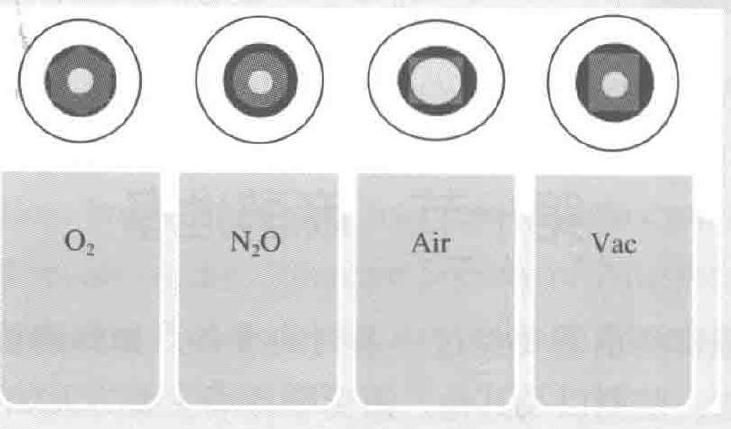
\includegraphics[max width=\textwidth]{2024_07_05_645bb794a4d4f32ee0c8g-068(1)}
\end{center}

图 3-1-1 不同气源墙壁接口形状

\section*{小贴士}
使用氧气瓶供氧前, 需要检查其出气口及减压器是否正确安装并旋紧, 打开氧气瓶阀, 确认氧气充足(图 3-1-2)。

\begin{center}
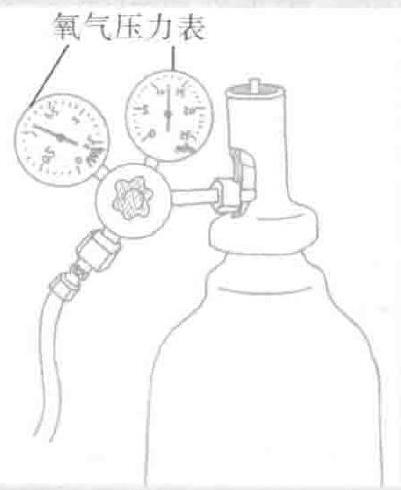
\includegraphics[max width=\textwidth]{2024_07_05_645bb794a4d4f32ee0c8g-068}
\end{center}

图 3-1-2 钢瓶氧气源使用注意事项

\begin{enumerate}
  \setcounter{enumi}{1}
  \item 高压系统 检查钢瓶或者中心供气系统气源:
\end{enumerate}

(1)开启钢瓶阀门, 证实钢瓶内至少有半筒的氧气容量 (如果使用钢瓶供氧)。

(2)关闭钢瓶阀门, 检查中央管道供气系统: 正确连接,压力在 $4 \mathrm{~kg} / \mathrm{cm}^{2}$ 左右。

\section*{3. 废气排放系统}
(1)确保废气排放系统与可调压力限制(APL)阀和呼吸机的排气阀准确无误连接。

(2)确认负压吸引系统的压力(必要时)。

(3)完全开大 APL 阀(0 $\mathrm{cm} \mathrm{H}_{2} \mathrm{O} )$ ,堵住 $\mathrm{Y}$ 形接口。

(4.)闭流量。

(5)按快速充氧钮, 回路内压力 $<10 \mathrm{~cm} \mathrm{H}_{2} \mathrm{O}$ 。

(6)检查废气排放系统的排气管是否通畅, 确保无扭曲堵塞现象。

\section*{4. 回路系统}
(1)氧浓度校正: a. 进行 $21 \%$ 氧的空气校正; b. 试验低氧报警功能; c. 将氧传感器插人呼吸回路, 进行快速充氧充盈呼吸回路, 氧浓度监测仪显示 $>90 \%$ 。

(2)检查呼吸回路的初始状态: a. 呼吸回路完整无损、无梗阻现象; b. 确认二氧化碳吸收罐内钠石灰有效, 在 “min”和 “max” 线之间。

(3)进行回路系统泄漏试验: a. 关闭流量计; b. 关闭 APL 阀, 堵住 $\mathrm{Y}$ 形接口; c. 快速充氧, 回路内压力至 $30 \mathrm{~cm} \mathrm{H}_{2} \mathrm{O}$ 左右; d. 至少维持压力 $10 \mathrm{~s}$; e. 打开 APL 阀,压力随之下降。

(4)检查呼吸机和单向阀: a.Y形接口连接模拟肺; b. 设定相应的呼吸参数; c. 设定为机械通气模式; d. 开启呼吸机,快速充氧, 使风箱充盈; e. 关闭所有气体流量; f. 证实风箱在吸气期能输出相应潮气量, 而呼气期能自动充满; g. 将新鲜气流设定为 $5 \mathrm{~L} / \mathrm{min}$; h. 证实呼吸机能使模拟肺充盈和相\\
应放空, 呼气末无过高的压力; i. 检查单向活瓣的活动正常; j. 呼吸回路的其他装置功能正常; k. 关闭呼吸机开关, 转换为手控呼吸模式 (Bag/APL)~1. 手控皮囊, 模拟肺张缩正常, 阻力和顺应性无异常; m. 移去 Y 形接口上的皮囊。

\begin{enumerate}
  \setcounter{enumi}{4}
  \item 麻醉机相关监测 检查、标定各种监测仪, 设定报警的上下限, 包括: 呼气末二氧化碳、脉率、氧饱和度、氧浓度分析、呼吸机容量监测(潮气量表)、气道压力监测。

  \item 检查后麻醉机的状态

\end{enumerate}

(1) 挥发器设置为关。

(2) APL 活瓣开放。

(3)呼吸模式设置为手控模式。

(4)所有流量表为零 (或为最小)。

(5)患者负压系统水平合适。

⑥患者回路系统准备妥当, 待用。

麻醉机工作原理见图 3-1-3。

\section*{二、器材准备}
\begin{enumerate}
  \item 全身麻醉器材准备 全身麻醉器材包括: 控制通气用具(呼吸回路和面罩), 建立气道用具(喉镜, 气管插管或喉罩、注射器、胶布, 图 3-1-4), 吸引器, 确定气管导管/喉罩位置用具(听诊器、呼气末二氧化碳监测), 根据需要选择口咽通气道、牙垫、胃管、薄枕等。
\end{enumerate}

实施麻醉前, 将插管用具置于洁净、有铺巾的方盘中备用。

\begin{enumerate}
  \setcounter{enumi}{1}
  \item 椎管内麻醉器材准备 椎管内麻醉器材包括消毒用具、穿刺用具、给药用具和置管用具(图 3-1-5)。

  \item 神经阻滞器材准备 神经阻滞器材包括消毒用具、定位用具、穿刺用具、给药用具, 并根据需要准备置管(图 3-1-6)。

\end{enumerate}

\begin{center}
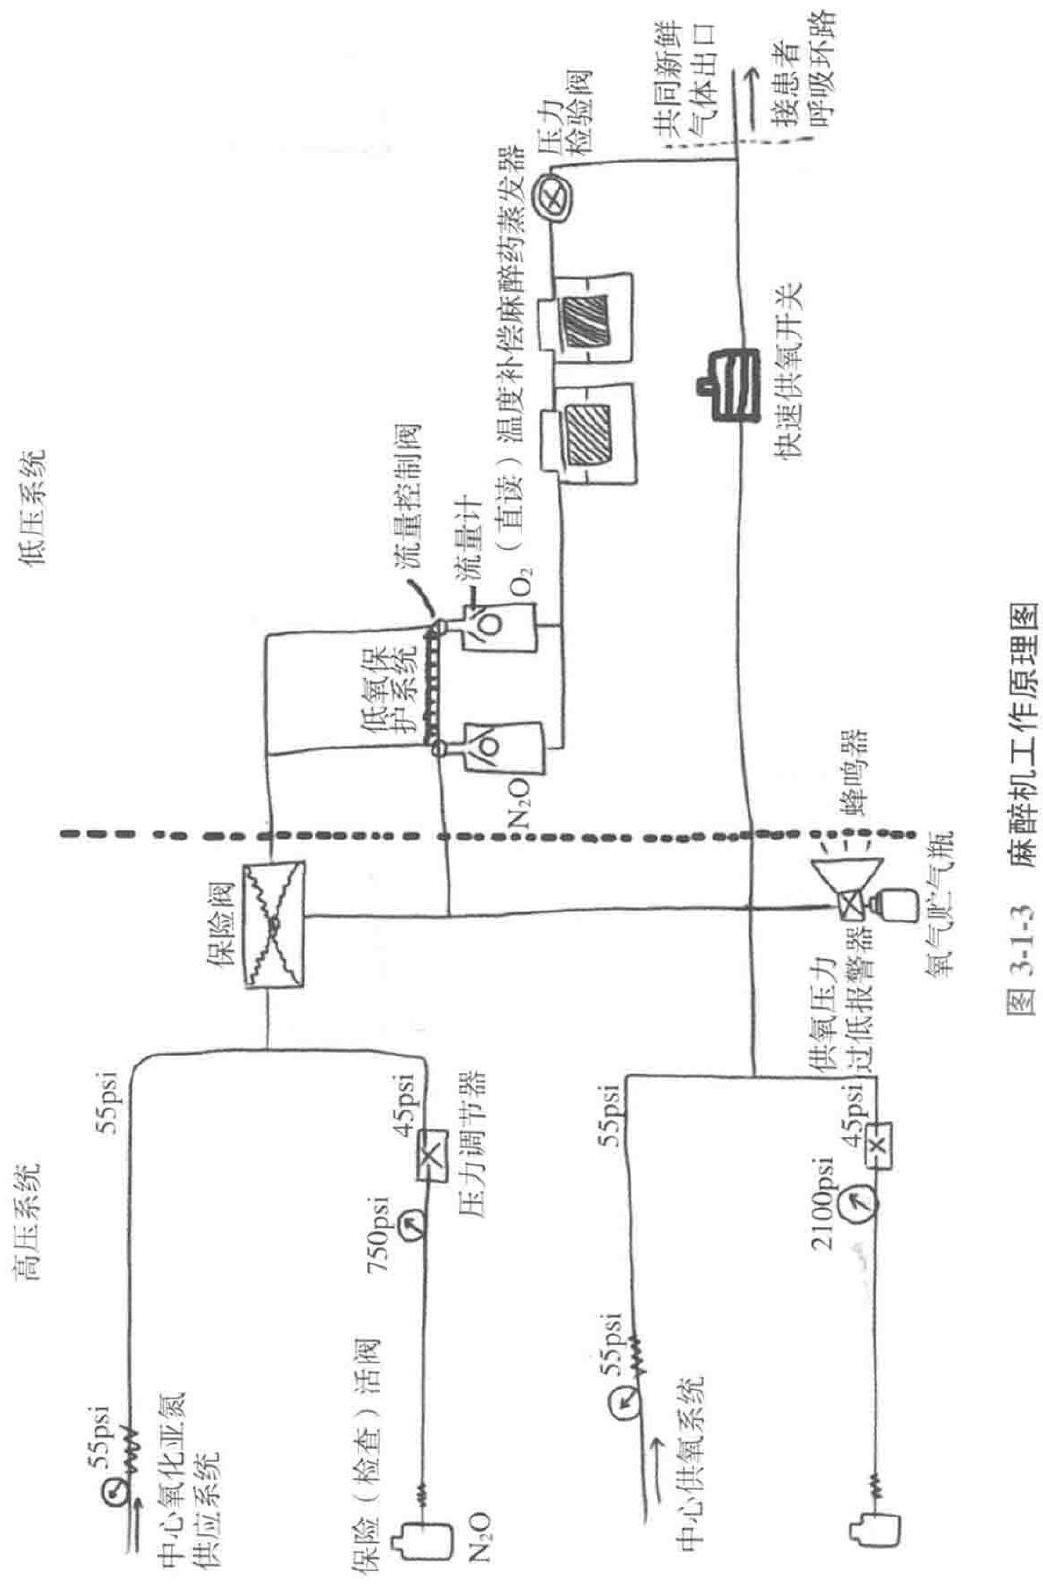
\includegraphics[max width=\textwidth]{2024_07_05_645bb794a4d4f32ee0c8g-071}
\end{center}

\section*{麻醉科住院医师手册}
\begin{center}
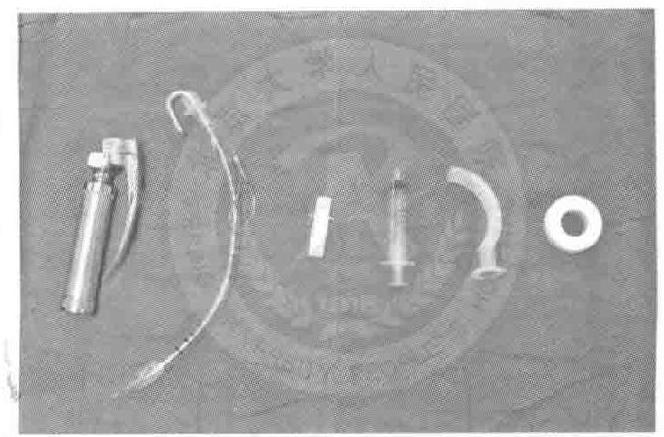
\includegraphics[max width=\textwidth]{2024_07_05_645bb794a4d4f32ee0c8g-072(1)}
\end{center}

图 3-1-4 气管插管用具

由左到右依次为喉镜、气管导管带导范、牙垫、注射器、口咽通气道、胶布

\begin{center}
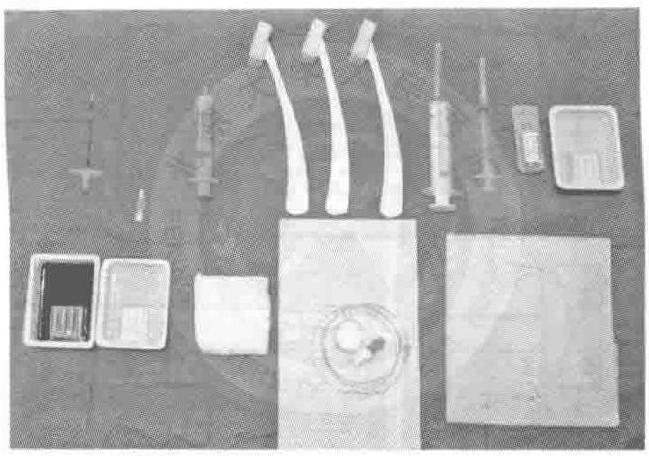
\includegraphics[max width=\textwidth]{2024_07_05_645bb794a4d4f32ee0c8g-072}
\end{center}

图 3-1-5 椎管内麻醉器材

上排由左到右:硬膜外针, 腰麻针, 低阻力注射器, 消毒刷, $20 \mathrm{ml}$ 空针, $2 \mathrm{ml}$空针, $2 \%$ 利多卡因,生理盐水;下排由左到右:碘伏和酒精(消毒后丢弃),纱布,硬膜外管,铺巾\\
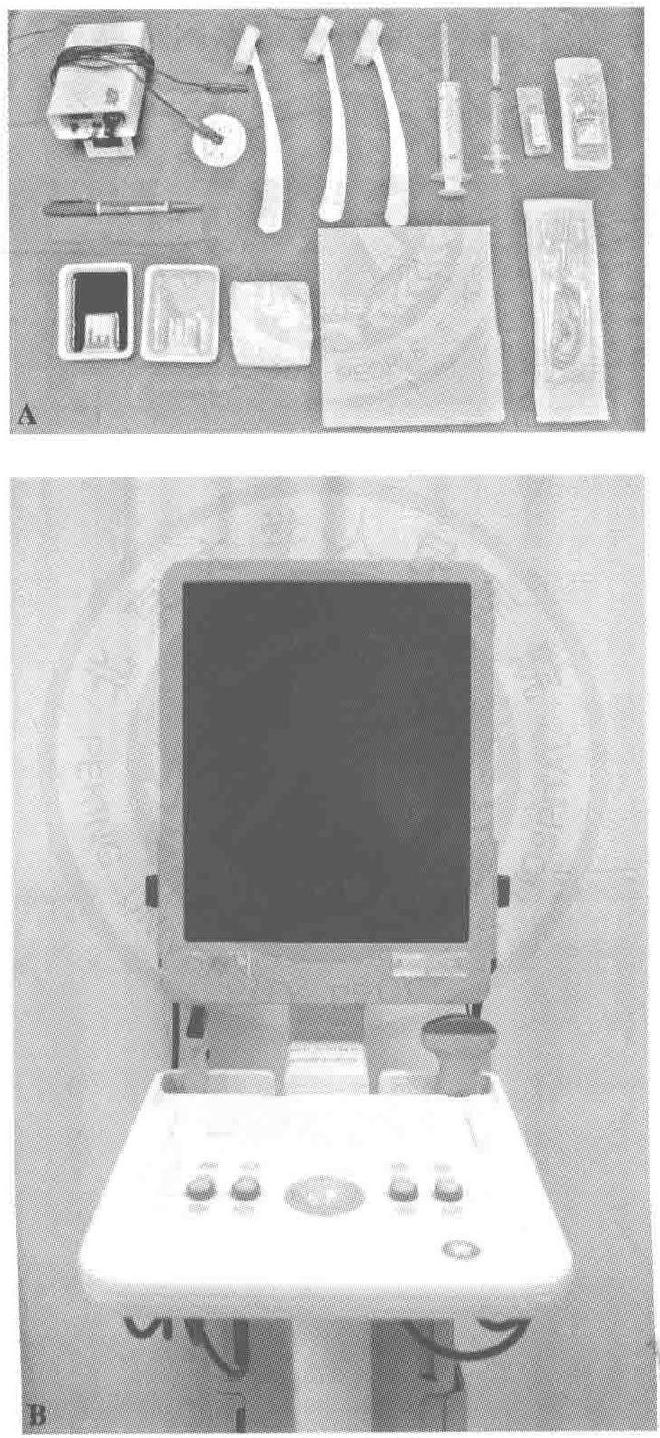
\includegraphics[max width=\textwidth, center]{2024_07_05_645bb794a4d4f32ee0c8g-073}

图 3-1-6 神经阻滞麻醉器材及超声仪

A. 上排由左到右: 神经刺激器及标记笔, 消毒刷, $20 \mathrm{ml}$ 及 $2 \mathrm{ml}$ 空针, 利多卡因, 罗哌卡因; 下排由左到右: 碘伏(消毒后丢弃), 生理盐水, 纱布, 铺巾,神经刺激针; B. 超声仪

\begin{enumerate}
  \setcounter{enumi}{3}
  \item 吸氧准备 吸氧需准备储氧面罩或鼻导管, 连接管 (图 3-1-7)。
\end{enumerate}

\section*{全身麻醉器材的准备清单}
\begin{itemize}
  \item 气管插管
\end{itemize}

通常女性 $7.0 \sim 7.5 \mathrm{mmID}$, 男性 $7.5 \sim 8.0 \mathrm{mmID}$

头颈部手术, 俯卧位手术需使用钢丝螺纹管

\begin{itemize}
  \item 喉罩
\end{itemize}

LMA 通常为女性3\#, 男性 4\#

\begin{itemize}
  \item 导芯

  \item 喉镜

\end{itemize}

Macintosh喉镜片,成人通常选用3 号

喉镜柄与喉镜片安装完成后打开检查光亮,弯折备用

・吸引器,吸痰管

\begin{itemize}
  \item 螺纠管(呼吸回路)
  \item 面罩
\end{itemize}

通常女性 4\#, 男性 5\#

\begin{itemize}
  \item 注射器

  \item 牙垫

  \item 胶布

  \item 口咽/鼻咽通气道

  \item 听诊器

\end{itemize}

\begin{center}
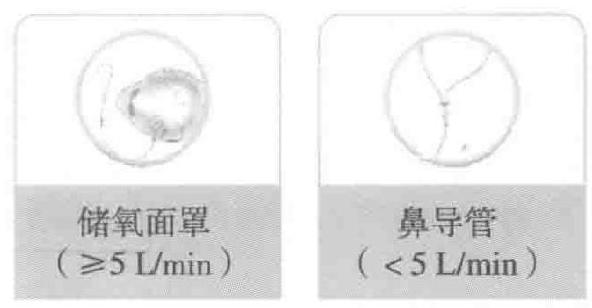
\includegraphics[max width=\textwidth]{2024_07_05_645bb794a4d4f32ee0c8g-075}
\end{center}

\section*{图 3-1-7 吸氧准备}
\section*{三、药物准备}
根据麻醉方式选择准备药物, 全身麻醉时需准备的全身麻醉药物包括镇静、镇痛、肌肉松驰三类药物; 椎管内麻醉及神经阻滞时, 需准备局部麻醉药物、镇静药物, 并可能需要镇痛药物; 局部麻醉 + 强化时, 则需要准备镇静、镇痛药物。所有麻醉均需准备基本的抢救药物及镇静药物。

\section*{1. 抢救及镇静药物}
\begin{itemize}
  \item 咪达夾仑
  \item 麻黄碱(通常稀释至 $6 \mathrm{mg} / \mathrm{ml}$ )
  \item 阿托品
\end{itemize}

\section*{2. 全身麻醉药物}
(1) 静脉全麻药

\begin{itemize}
  \item 丙泊酚
  \item 依托味酯
\end{itemize}

(2) 镇痛药

\begin{itemize}
  \item 芬太尼
  \item 舒芬太尼(通常稀释至 $5 \mu \mathrm{g} / \mathrm{ml}$ )
  \item 瑞芬太尼(通常稀释至 $20 \mu \mathrm{g} / \mathrm{ml}$ 或 $40 \mu \mathrm{g} / \mathrm{ml}$ )
\end{itemize}

(3) 肌肉松驰剂

\begin{itemize}
  \item 罗库溴铵
  \item 顺阿曲库铵
  \item 哌库溴铵
\end{itemize}

(4. 吸人麻醉药

\begin{itemize}
  \item 七氟烷
  \item 异氟烷
  \item 地氟烷
\end{itemize}

\section*{小贴士}
给麻醉机加入吸入麻醉药时,需要注意:核对药品和挥发罐名称是否一致, 关闭挥发罐后再操作, 使用加药器以防药物泄漏污染环境(图 3-1-8)。加药量勿超过加药器最高刻度,否则会喷酒。\\
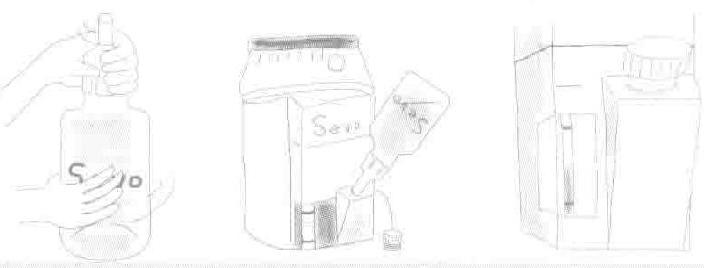
\includegraphics[max width=\textwidth, center]{2024_07_05_645bb794a4d4f32ee0c8g-076}

图 3-1-8 麻醉机加药注意事项

\section*{3. 椎管内麻醉及神经阻滞用药}
\begin{itemize}
  \item 利多卡因
  \item 布比卡因(丁哌卡因)
  \item 罗哌卡因
\end{itemize}

\section*{四、监测}
\begin{enumerate}
  \item 基本监测 对于所有接受麻醉的患者,基本监测包括无创血压、 3 导联心电图、无创血氧饱和度。对于控制通气的患者, 需要进行呼气末二氧化碳监测。对于手术时间长于 $2 \mathrm{~h}$, 行开胸、开腹手术,或者有大出血或重症患者,均应\\
进行体温监测。

  \item 特殊监测 根据患者情况, 可选择的监测手段还包括: 有创血压、中心静脉压、脑电双频指数(BIS)、经食管超声心动图(TEE)、肺动脉压(PAP)监测等(图 3-1-9)。\\
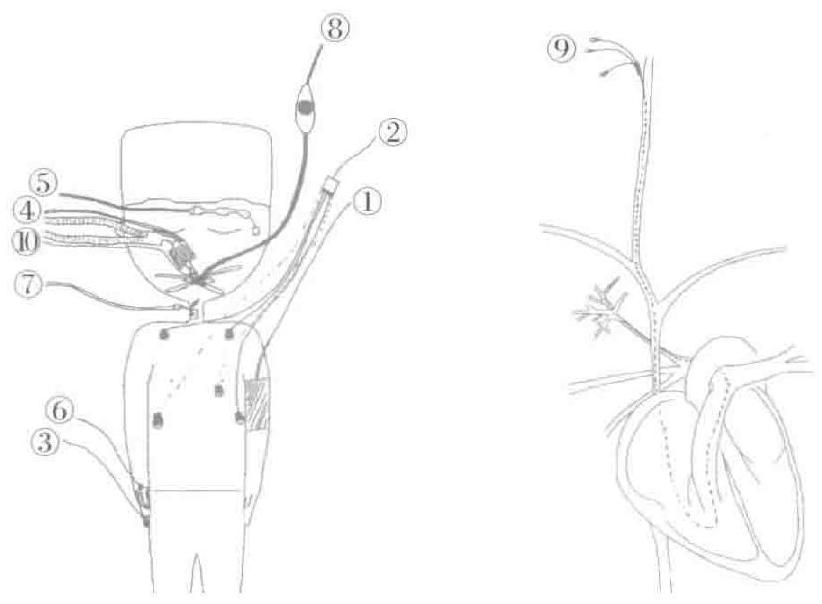
\includegraphics[max width=\textwidth, center]{2024_07_05_645bb794a4d4f32ee0c8g-077}

\end{enumerate}

图 3-1-9 术中监测的示意图

(1) 袖带, (2)心电图 (实线为 3 导联, 虚线为 5 导联中另外 2 个导联), (3)脉搏氧饱和度, (4)气体采样管, (5) BIS, (6)有创动脉压力监测管, (7)中心静脉置管, (8) TEE, (9) PAP (虚线为在人体内走行), 100咁温

\section*{五、小结}
麻醉准备内容可用麻醉前准备清单来概括。

\section*{麻醉前准备清单}
\begin{itemize}
  \item 患者对麻醉及手术不存在特殊问题,签署知情同意书
  \item 义齿、助听器、隐形眼镜、首饰、手表、手机等一切物品已取走
  \item 确认禁食、禁水时间(表 3-1-1)
\end{itemize}

\section*{麻醉前准备清单}
\begin{itemize}
  \item 确认最近的检查结果、病情变化
  \item 监测已经开始
  \item 输液通畅
  \item 麻醉机;气源准备就绪(表 3-1-2)
  \item 药物准备就绪
  \item 确认拟行手术种类, 手术医生到位, 手术器械及敷料已准备好
\end{itemize}

表 3-1-1 禁食、禁水时间 ${ }^{(1)}$

\begin{center}
\begin{tabular}{|c|c|c|}
\hline
种类 & 时间 (h) & 备注 \\
\hline
透明饮料 & 2 & \multirow{5}{*}{}\begin{tabular}{l}
- 㛝儿及新生儿禁食 $2 \mathrm{~h}$ 后需要 \\
静脉输注含棭体 \\
- 术前需口服用药者, 允许在 \\
术前 $1 \sim 2 \mathrm{~h}$ 服药, 并饮人 \\
$0.25 \sim 0.5 \mathrm{ml} / \mathrm{kg}$ 清水 \\
\end{tabular} \\
\hline
母乳 & 4 &  \\
\hline
牛奶/配方奶 & 6 &  \\
\hline
淀粉类固体食物 & 6 &  \\
\hline
脂肪类固体食物 & 8 &  \\
\hline
\end{tabular}
\end{center}

表 3-1-2 机械通气的常用设置

\begin{center}
\begin{tabular}{ll}
机械通气参数 & 常用设置 \\
\hline
潮气量 (tidal volume, TV) & \begin{tabular}{l}
$6 \sim 8 \mathrm{ml} / \mathrm{kg}$ \\
(小儿 $8 \sim 10 \mathrm{ml} / \mathrm{kg}$ ) \\
\end{tabular} \\
频率 (frequency, f) & $10 \sim 12$ 次 $/$ 分 \\
 & (小儿 次/分) \\
吸呼比 (I : E) & $1: 2 \sim 1: 1.5$ \\
呼气末正压 & $0 \sim 5 \mathrm{~cm} \mathrm{H} \mathrm{H}_{2} \mathrm{O}$ \\
(positive end-expiratory pressure, PEEP) &  \\
新鲜气体流量 (fresh gas flow, FGF) &  \\
紧闭麻醉 &  \\
半紧闭麻醉 & $0.5 \sim 1 \mathrm{~L} / \mathrm{min}$ \\
\hline
\end{tabular}
\end{center}

\section*{小贴士}
\section*{安装静脉泉要点(图 3-1-10):}
\begin{itemize}
  \item 连接外接电源
  \item 扣实所有卡位
  \item 针管刻度及标签均朝外
\end{itemize}

\begin{center}
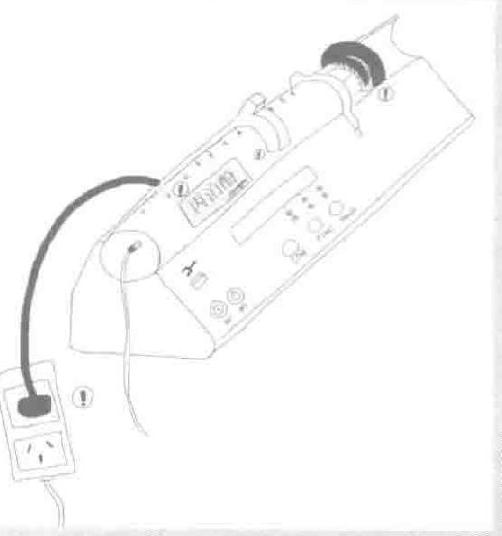
\includegraphics[max width=\textwidth]{2024_07_05_645bb794a4d4f32ee0c8g-079}
\end{center}

图 3-1-10 安装静脉泉要点

\section*{参考文献}
\begin{enumerate}
  \item 中华医学会麻醉学分会. 中国麻醉学指南与专家共识 (2014版).北京:人民卫生出版社,2014:73-75.
\end{enumerate}

\[
\text { (田雪 乔青 冯艺) }
\]

麻醉科住院医师手册

\begin{center}

\includegraphics[max width=\textwidth]{2024_07_05_645bb794a4d4f32ee0c8g-080(19)}
\end{center}

为减少手术失误,世界卫生组织(WHO)于 2008 年患者安全行动中提出“安全手术㧺救生命”,将在全球推行严格规范外科手术各阶段的标准, 并推出了一份外科手术安全指南(手术安全核查表),希望以此推动各国提高手术安全,避免每年成千上万人因手术后的并发症而死亡。图 3-2-1 为北京大学人民医院使用的三方核查表。

**医院手术安全核查表

\begin{center}
\begin{tabular}{|c|c|c|}
\hline
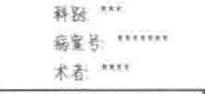
\includegraphics[max width=\textwidth]{2024_07_05_645bb794a4d4f32ee0c8g-080(7)}
 & 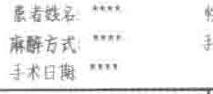
\includegraphics[max width=\textwidth]{2024_07_05_645bb794a4d4f32ee0c8g-080(15)}
 & 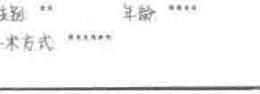
\includegraphics[max width=\textwidth]{2024_07_05_645bb794a4d4f32ee0c8g-080(36)}
 \\
\hline
麻酰实施前 & 手犬开始前 & 患者严手术室前 \\
\hline

\includegraphics[max width=\textwidth]{2024_07_05_645bb794a4d4f32ee0c8g-080(1)}
 & 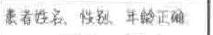
\includegraphics[max width=\textwidth]{2024_07_05_645bb794a4d4f32ee0c8g-080(23)}
 & 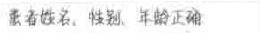
\includegraphics[max width=\textwidth]{2024_07_05_645bb794a4d4f32ee0c8g-080(32)}
 \\
\hline
$口$ 是㧹 & $口$ 昆 $\square$ 各 & $口$ 是 \\
\hline
乎术方式唃狁:昆口否 & 手术方式确认㖷 $\square$ 自 & 
\includegraphics[max width=\textwidth]{2024_07_05_645bb794a4d4f32ee0c8g-080(31)}
 \\
\hline
手术暗位与标识正能 & 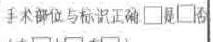
\includegraphics[max width=\textwidth]{2024_07_05_645bb794a4d4f32ee0c8g-080(22)}
 & 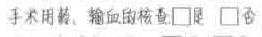
\includegraphics[max width=\textwidth]{2024_07_05_645bb794a4d4f32ee0c8g-080(4)}
 \\
\hline
$口$ 是 口否 & $(t \square+\square$ 涼 & 手耒㭌物青点正维 $\square$ 是 $\square$ 合 \\
\hline
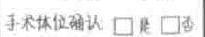
\includegraphics[max width=\textwidth]{2024_07_05_645bb794a4d4f32ee0c8g-080(6)}
 & 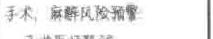
\includegraphics[max width=\textwidth]{2024_07_05_645bb794a4d4f32ee0c8g-080(5)}
 & 
\includegraphics[max width=\textwidth]{2024_07_05_645bb794a4d4f32ee0c8g-080(12)}
 \\
\hline
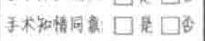
\includegraphics[max width=\textwidth]{2024_07_05_645bb794a4d4f32ee0c8g-080(30)}
 & 子不医情特过 & 
\includegraphics[max width=\textwidth]{2024_07_05_645bb794a4d4f32ee0c8g-080(21)}
 \\
\hline

\includegraphics[max width=\textwidth]{2024_07_05_645bb794a4d4f32ee0c8g-080(18)}
 & 预计手术时同 $\square$ & 
\includegraphics[max width=\textwidth]{2024_07_05_645bb794a4d4f32ee0c8g-080(9)}
 \\
\hline

\includegraphics[max width=\textwidth]{2024_07_05_645bb794a4d4f32ee0c8g-080(10)}
 & 
\includegraphics[max width=\textwidth]{2024_07_05_645bb794a4d4f32ee0c8g-080(26)}
 & $\square$ 是 \\
\hline

\includegraphics[max width=\textwidth]{2024_07_05_645bb794a4d4f32ee0c8g-080(27)}
 & 
\includegraphics[max width=\textwidth]{2024_07_05_645bb794a4d4f32ee0c8g-080(34)}
 & 名袖㝍漛 \\
\hline
$\square$ 是 $\square$ 즘 & 
\includegraphics[max width=\textwidth]{2024_07_05_645bb794a4d4f32ee0c8g-080(13)}
 & 珬期通治 $\square$ \\
\hline

\includegraphics[max width=\textwidth]{2024_07_05_645bb794a4d4f32ee0c8g-080(20)}
 & 麻餅米技这口 & 气括考 $\square$ \\
\hline

\includegraphics[max width=\textwidth]{2024_07_05_645bb794a4d4f32ee0c8g-080(14)}
 & H他 $\square$ & क口引为口 $\square$ \\
\hline

\includegraphics[max width=\textwidth]{2024_07_05_645bb794a4d4f32ee0c8g-080(2)}
 & 
\includegraphics[max width=\textwidth]{2024_07_05_645bb794a4d4f32ee0c8g-080(16)}
 & \%娄 $\square$ \\
\hline

\includegraphics[max width=\textwidth]{2024_07_05_645bb794a4d4f32ee0c8g-080(24)}
 & 抱苌不票合楼口 & 原唡 $\square$ \\
\hline
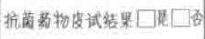
\includegraphics[max width=\textwidth]{2024_07_05_645bb794a4d4f32ee0c8g-080(3)}
 & 仅罧设学口 & 
\includegraphics[max width=\textwidth]{2024_07_05_645bb794a4d4f32ee0c8g-080(8)}
 \\
\hline
术前各传 $\square$ 是 $\square$ 要 & 
\includegraphics[max width=\textwidth]{2024_07_05_645bb794a4d4f32ee0c8g-080(11)}
 & H他 \\
\hline
粮带信息校对 $\square$ 是 $\square$ 否 & 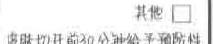
\includegraphics[max width=\textwidth]{2024_07_05_645bb794a4d4f32ee0c8g-080(17)}
 & 欪者去同: \\
\hline
椵体 $\square$ /你白植入物 $\square$ / & \includegraphics[max width=\textwidth]{2024_07_05_645bb794a4d4f32ee0c8g-080}
 & \includegraphics[max width=\textwidth]{2024_07_05_645bb794a4d4f32ee0c8g-080(29)}
 \\
\hline
影佳学寅杫口 & \includegraphics[max width=\textwidth]{2024_07_05_645bb794a4d4f32ee0c8g-080(35)}
 & \includegraphics[max width=\textwidth]{2024_07_05_645bb794a4d4f32ee0c8g-080(28)}
 \\
\hline
其他: & H他: &  \\
\hline
手术断豚: & 手太医师。 & 手术㗨帅 \\
\hline
\includegraphics[max width=\textwidth]{2024_07_05_645bb794a4d4f32ee0c8g-080(33)}
 & 床部性 & \includegraphics[max width=\textwidth]{2024_07_05_645bb794a4d4f32ee0c8g-080(25)}
 \\
\hline
手术室接む & 子术效护む & 手求要护士 \\
\hline
\end{tabular}
\end{center}

图 3-2-1 三方核查表

\section*{第三节 全身麻醉的诱导、维持和苏醒}
\section*{麻醉要素清单}
\begin{itemize}
  \item 意识消失
  \item 镇痛
  \item 肌肉松弛
  \item 抑制不良应激反应
\end{itemize}

理想的全身麻醉应做到:在保证患者安全的同时, 使其意识消失、充分镇痛、肌肉松弛, 并且有效降低不良应激反应。

\section*{一、麻醉诱导}
麻醉诱导的目的是让患者平稳进人麻醉状态,并且减轻麻醉操作(如气管内插管)时的应激反应。

患者进行诱导前应确认做好所有相应的准备(见 63 页 “麻醉前准备清单”),确认可以麻醉并手木。

\section*{(一) 静脉诱导}
\begin{enumerate}
  \item 调整体位 枕部垫一薄枕 (厚约 $10 \mathrm{~cm}$ ), 颈后仰 (图 3-3-1)。

  \item 给氧去氮 纯氧面罩通气, 令患者深呼吸 $3 \mathrm{~min}$ 。

  \item 给麻醉药物 一般包括静脉全身麻醉、镇痛、肌肉松驰三类药物。

  \item 逐渐由自主呼吸过渡为人工辅助通气及人工控制通气。

  \item 待药效均达峰值时, 建立人工气道(气管内插管、喉罩置人等)。

\end{enumerate}

\begin{center}
\includegraphics[max width=\textwidth]{2024_07_05_645bb794a4d4f32ee0c8g-082}
\end{center}

图 3-3-1 诱导时, 患者平卧位, 可枕薄枕, 患者头部位于床边缘, 床高度应适中

\section*{小贴士}
$\sqrt{ }$ 诱导时, 床面与麻醉医师的剑突在同一水平面利千操作。 $\checkmark$ 患者未入睡时应轻扣面罩, 不要紧压面罩造成患者紧张。 $\checkmark$ 患者清醒状态下, 肌松药起效可能造成恐惧、濒死感,因此常在意识消失后再给予肌松药。

$\checkmark$ 给予阿片类药物时, 需注意不要过快给药, 以免造成不必要的肌紧张、呛咳等情况。

$\checkmark$ 插管时机:所有诱导药物的药效达高峰时。

诱导过程中需严密监测, 根据患者情况增减药物种类或剂量。

\section*{(二)吸入诱导}
\begin{enumerate}
  \item 调整体位 参见 “静脉诱导”。

  \item 给氧去氮 参见 “静脉诱导”。

\end{enumerate}

\section*{3. 诱导方法}
(1)浓度递增慢诱导法: APL 阀处于开放状态, 氧流量\\
$6 \sim 8 \mathrm{~L} / \mathrm{min}$, 起始刻度为 $0.5 \%$, 每 3 4 次呼吸增加 $0.5 \%$,直至达到所需要的麻醉 / 镇静深度。

(2)潮气量法: 吸纯氧 $3 \mathrm{~min}$ 后, 吸人高浓度麻醉药, 患者平静呼吸, 直至达到所需麻醉 / 镇静深度。

(3)肺活量法: 适用于 6 岁以上能配合的患者, 回路预充麻醉气体, 患者深呼气后深吸气, 吸人高浓度麻醉药, 之后屏气,20~ $40 \mathrm{~s}$ 后意识消失。

\begin{enumerate}
  \setcounter{enumi}{3}
  \item 观察患者呼吸频率及潮气量, 并调节吸入药物浓度,必要时辅助通气。

  \item 待达到满意的麻醉深度时, 建立人下气道。

\end{enumerate}

\section*{小贴士}
\includegraphics[max width=\textwidth, center]{2024_07_05_645bb794a4d4f32ee0c8g-083}\\
量, 并排空储气囊 3 次, 使回路内预充高浓度麻醉药,缩短诱导时间。

$\checkmark$ 患者苏醒后通常只能记得第一次吸气, 尽管其是通过多次深呼吸才能达到麻醉状态。

\section*{(三)快速序贯诱导}
\begin{enumerate}
  \item 调整体位 参见 “静脉诱导”。

  \item 给氧去氮 参见 “静脉诱导”。由于快速序贯诱导常应用于饱胃患者, 应尽量避免面罩加压给氧, 此时吸纯氧去氮尤其重要, 并应尽量持续至肌松药起效, 准备粗口径吸引器并处于备用状态。

  \item 选择起效快、消除快的麻醉药物,患者意识消失后,令助手压迫患者的环状软骨。

  \item 肌松药起效后立刻建立人工气道, 并立即给了套囊充气。

\end{enumerate}

\section*{麻醉科住院医师手册}
\section*{(四)清醒插管}
\begin{enumerate}
  \item 与患者充分沟通 告知患者插管过程中可能面临的不适。

  \item 声门上表面麻醉 将 $1 \%$ 丁卡因或 $2 \%$ 利多卡因喷洒于舌根及咽喉, 待舌根麻醉起效后, 可用喉镜轻轻挑起舌体,用局麻药喷洒声门。

  \item 声门下表面麻醉 将配好局麻药的注射器经环甲膜刺入(图 3-3-2)。若回抽有气体, 则表明针尖已进人气管内。快速注射局麻药。拔针并以棉签压迫针孔,令患者咳嗽, 使局麻药均匀分布于声门下气管表面。

\end{enumerate}

\begin{center}
\includegraphics[max width=\textwidth]{2024_07_05_645bb794a4d4f32ee0c8g-084}
\end{center}

图 3-3-2 环甲膜穿刺部位

\begin{enumerate}
  \setcounter{enumi}{3}
  \item 给予少量镇静、镇痛药物后, 进行插管, 可用光棒、纤维支气管镜(纤支镜)等辅助。确认气道成功建立后, 进行麻醉诱导。
\end{enumerate}

\section*{二、麻醉操作结束至手术切皮时}
手术开始前, 需要确认达到足够的麻醉深度, 并根据手\\
术刺激强度和给药间隔时间决定是否追加镇痛、镇静、肌松药, 调整静脉麻醉药或吸人麻醉药。

\section*{小贴士}
$\checkmark$ 在摆体位、消毒过程中, 由于缺少刺激, 麻醉深度常相对较深,但不代表麻醉深度足以满足手术应激的要求。

$、$ 若患者出现体动、自主呼吸(呼气未二氧化碳波形切迹)、流泪、血压升高、心率加快等,表明麻醉过浅,应该避免。

\section*{三、麻醉维持}
在麻醉维持过程中,仍需从意识消失、镇痛、肌松及应激反应四个方面考虑, 同时应根据患者状态、手术 / 疾病需要以及转归需求做综合处理。

无论通过全身麻醉、椎管内麻醉、区域阻滞、局部浸润、镇静等方法, 还是复合两种及以上麻醉方式, 均可达到维持满意麻醉的目的。需要注意:麻醉的 4 个要素既是一个整体, 又需要分别考虑。不宜通过单纯加大全麻药剂量来抵消疼痛刺激的增加或肌肉紧张, 而应尽量全面地根据患者状态和手术需要调整针对 4 个要素的麻醉实施。同时, 复合麻醉常相互协同, 如硬膜外麻醉复合全身麻醉时, 所需的硬膜外麻醉药量和全身麻醉药量均应减少。不同原理的麻醉药物之间有复杂的相互作用方式,临床麻醉常用的药物作用以协同为主, 例如应用阿片类药物后, 达到相同镇静深度所需的镇静药物也会减少。充分的区域阻滞、神经阻滞和局部浸润有时可起到良好的抑制不良反射的效果。

\section*{(一) 呼吸状态}
\begin{enumerate}
  \item 维持 $\mathrm{SpO}_{2}>95 \%$ 。

  \item 维持 $\mathrm{P}_{\mathrm{ET}} \mathrm{CO}_{2} 30 \sim 45 \mathrm{mmHg}$ 。

\end{enumerate}

\section*{3. 气道压 $<20 \mathrm{~cm} \mathrm{H}_{2} \mathrm{O}$ 。}
\begin{enumerate}
  \setcounter{enumi}{3}
  \item 关注麻醉机工作状态, 不要在未了解报警原因的情况下关闭警报。
\end{enumerate}

\section*{(二)循环状态}
\begin{enumerate}
  \item 维持血压 $>90 / 60 \mathrm{mmHg}$ (或根据基础疾病和手术需要调整标准)。

  \item 如为有创动脉血压, 可根据波形、基线随呼吸变化大致判断容量状态(见本章第五节“麻醉监测”)。

  \item 维持心率 $60 \sim 100$ 次 / 分, 律齐(或根据基础疾病和手术需要调整标准)。

  \item 维持中心静脉压(central venous pressure, CVP)5~ $10 \mathrm{~cm} \mathrm{H}_{2} \mathrm{O}$ (或根据基础疾病和手术需要调整标准)。

  \item 尿量 $>0.5 \sim 1 \mathrm{ml} /(\mathrm{kg} \cdot \mathrm{h})$ 。

  \item 触摸肢端温暖干燥, 表示末梢灌注好; 若为湿冷, 则提示木梢灌注不良。

  \item 若监测连续心排血量 (continuous cardiac output, $\mathrm{CCO}$ )、肺动脉压(pulmonary artery pressure, PAP)、每搏变异指数(stroke volume variation, SVV), 则维持三者在正常范围内或根据基础疾病和手术需要调整标准。

  \item 经食管超声心动图(transesophageal echocardiography, TEE)可观察并定量判断心肌收缩和舒张功能, 以及是否存在瓣膜反流或其他病变(见本章第五节“麻醉监测”)。

\end{enumerate}

\section*{(三)容量平衡}
\begin{enumerate}
  \item 出血量。

  \item 尿量(每 $2 \mathrm{~h}$ 至少记录一次尿量, 休克、出血时以及利尿处理前后需加强监测)。

  \item 观察术野(腹水、渗血、渗出液等)。

  \item 观察结膜、皮肤、肠壁等是否有水肿表现。

  \item 除输液量外, 还需要注意输液速度。老年、小儿、心功能障碍等患者, 不宜输液过快; 大出血时, 则应考虑加压输液输血以快速补充血容量。

  \item 可以通过 CVP、SVV、TEE 等方法辅助判断容量是否合适。

\end{enumerate}

\section*{(四)麻醉深度}
\begin{enumerate}
  \item 心率、血压、体动、应激反应可辅助判断麻醉深度是否合适。

  \item BIS、EEG 等监测可辅助判断麻蟀深度。

\end{enumerate}

\section*{(五)肌肉松驰}
\begin{enumerate}
  \item 全身麻醉过程中, 应保证患者无手术刺激引起的体动。

  \item 控制呼吸时, 应使患者无自主呼吸。

  \item 对于开腹、开胸等术式, 在保证安全的前提下, 应尽量为术者创造条件, 令肌肉足够松驰, 同时有助于避免手,术损伤, 减小应激。

\end{enumerate}

\section*{(六)镇痛}
多采用阿片类药物镇痛, 可静脉持续输注超短效的瑞芬太尼, 但仍应间断补充中长效镇痛药物, 以避免疼痛的反弹及超敏反应。

\section*{(七)体温}
\begin{enumerate}
  \item 对开胸、开腹术式, 小儿、休克、头颈部手术、颎脑病变、大出血以及任何时间长于 $2 \mathrm{~h}$ 的手术的患者, 均应做体温监测。

  \item 对可以预见的低体温患者, 应在体温下降前采取保温措施。

  \item 体外循环下的手术通常需要分别监测顾脑温度 (鼻咽温)和中心温度(直肠或膀胱温), 并根据手术阶段采取升温或降温措施。

\end{enumerate}

\section*{(八)术中实验室检查}
\begin{enumerate}
  \item 血气分析(大出血、休克、长时间手术,或者任何需要解释呼吸功能障碍、怀疑电解质酸碱失衡的情况)。

  \item 凝血功能检查(肝移植或怀疑凝血功能异常时)。

  \item 血糖(糖尿病、体外循环等情况)。

\end{enumerate}

\section*{小贴士}
$\checkmark$ 任何监测指标都应该设定报警值, 在麻醉过程中监测超出报警值时, 可被听到。

$\checkmark$ 脉氧的频率及音调可提供心率、心律、血氧饱和度等信息。

$\checkmark$ 麻醉医生应将监测及麻醉机显示屏摆放在方便随时查看的位置。

\section*{通气模式 (图 3-3-3 ) 注解}
$\checkmark$ 容量控制通气(volume controlled ventilation, VCV)最常用。

$\checkmark$ 压力控制通气(pressure controlled ventilation,PCV)适用于各种原因气道压升高的患者、小儿患者, 可避免气压伤。

$\checkmark$ 同步间歇通气 (synchronized intermittent mechanical ventilation, SIMV)。

$\sqrt{ }$ 压力支持通气(pressure support ventilation, PSV)和 SIMV 的使用前提是患者有自主呼吸但潮气量不足的情况。适用于保留自主呼吸的全身麻醉或机械通气与自主呼吸的过渡。

\section*{小贴士}
$\checkmark$ 持续正压通气 (continuous positive airway pressure, CPAP)常用于単肺通气经调节呼吸参数仍不能维持氧合时病肺的通气。

$\checkmark$ 呼气末正压通气(positive end-expiratory pressure, PEEP)使呼气未小气道开放, 常用于治疗低氧血症。\\
\includegraphics[max width=\textwidth, center]{2024_07_05_645bb794a4d4f32ee0c8g-089}

图 3-3-3 四种常用机械通气示意图

四、麻醉苏醒

当停止使用全身麻醉药后, 药物浓度在体内逐渐下降,直至恢复意识。药物浓度下降的速度取决于药物的半衰期,当持续输注或多次间断输注时,则取决于时-量相关半衰期。通常来说,半衰期长的药物,时-量相关半衰期也长。

\section*{气管拔管以及术后转归内容详见第 4 章“术后管理”。}
\[
\text { (田雪 乔青 鞠辉) }
\]

\section*{第四节 监护性麻醉}
监护性麻醉(monitored anesthesia care, MAC)是指静脉镇静、麻醉和局部麻醉相结合的麻醉技术, 即在局部麻醉期间, 由麻醉医师负责实施镇静、镇痛, 并监测患者的生命体征。

\section*{一、目的}
\begin{enumerate}
  \item 消除患者的焦虑, 并让患者遗忘术中发生的不适和恐惧。

  \item 缓解疼痛和其他伤害性刺激。

\end{enumerate}

\section*{二、适应证}
在局部麻醉或区域阻滞下施行外科手术或各种诊断治疗性操作。如:消化道内镜或纤维气管镜的检查和治疗, 血管造影, 介入性治疗, 牙科、眼科、耳鼻喉科手术, 体外碎石, 儿科影像术, 体表及其他整形外科手术, 关节镜及肢体手术,膀胱镜检查及手术等。

\section*{三、麻醉前准备}
\begin{enumerate}
  \item 常规行病史回顾、体检和必要的实验室检查。

  \item 术前常规禁食、禁水。

  \item 对于 ASA III 〜IV 级的患者必须确定目前的生理状态是否适宜择期手术,需进行何种实验室检查和特殊处理。

\end{enumerate}

\section*{四、常用药物}
\begin{enumerate}
  \item MAC 期间, 应根据不同手术或操作的要求, 选择不同的镇静和(或)镇痛药物。

  \item 所选药物应具备以下特点:起效快; 对呼吸、循环干扰小; 消除方式不依赖于肝、肾功能, 消除半衰期短; 代谢产物无生物学活性;停药后恢复快。

\end{enumerate}

\section*{3. 常用药物}
(1)镇静 - 抗焦虑药:地西泮、咪达唑仑、丙泊酚、依托咪酯等。

(2)阿片类镇痛药:吗啡、芬太尼、阿芬太尼、瑞芬太尼等。

(3)其他镇痛药:氯胺酮、曲马多、NSAIDs 药物。

其中丙泊酚和短效的阿片类镇痛药以其独特的药效学特点在 MAC 时得以广泛应用。

\begin{enumerate}
  \setcounter{enumi}{3}
  \item 用药方式 单次静脉注射, 持续泵人, 靶控输注 (TCI),患者自控镇痛(PCA),患者自控镇静(PCS)等。
\end{enumerate}

\section*{五、术中监测与管理}
MAC 的基本监测与全身麻醉相同,包括:

\begin{enumerate}
  \item 专职麻醉医师全程监测。

  \item 监测呼吸功能: 脉搏氧饱和度、呼吸频率和幅度。必要时, 行鼻导管监测 $\mathrm{EtCO}_{2}$ 。

  \item 监测循环功能:持续监测 ECG、血压和心率。

  \item 并发症的观察和处理, 如恶心、呕吐、注射痛等。

\end{enumerate}

\section*{六、患者离室的标准}
\begin{enumerate}
  \item 意识完全清醒, 能按指令活动。

  \item 各种保护性反射恢复。

  \item 呼吸、循环功能稳定。

  \item 能自主站立; 对于无站立能力者,应恢复到术前水平。

\end{enumerate}

\section*{七、注意事项}
\begin{enumerate}
  \item 术中镇静、镇痛药的使用不应妨碍患者口头交流或呼吸道保护的能力。

  \item 常规的监测和急救装置必须随手可得, 一旦出现并发症应及时处理。

\end{enumerate}

\section*{第五节 麻醉监测}
直接观察患者仍是最重要的, 有经验的麻醉医师通常能通过最基本的观察对患者情况做出大致判断。监测仪器的数据则可提供进一步的参考。

\section*{一、直接观察}
直接观察包括基本的视、触、吒、听。

\section*{(一) 视}
\begin{enumerate}
  \item 出血 出血量需要通过吸引器内容量、浸湿纱布数量、患者疾病情况(有无腹水、渗液等)来综合确认。同时,应关注术野有无血块或持续渗血来判断患者凝血状态。

  \item 皮肤 正常的皮肤应为红润、温暖、干燥。皮肤湿冷提示微循环障碍, 发汗提示可能是低血糖、自主神经紊乱的症状, 苍白提示贫血, 潮红、出现皮疹则可能是过敏的征兆, 青紫提示血氧饱和度严重降低, 花斑提示可能为严重的供血不足。

  \item 静脉 可通过颈静脉是否充盈来间接评估循环血量是否充足, 颈静脉怒张可帮助粗略判断是否存在严重的右心功能不全、心脏压塞等。

  \item 呼吸 自主呼吸时可通过胸廓起伏判断呼吸是否规则, 并判断潮气量是否足够。当出现舌后坠时, 吸气可出现三凹征。辅助通气或机械通气时, 应通过胸廓起伏判断气道是否通畅。

  \item 麻醉深度 应用阿片类药物后瞳孔缩小, 可辅助判断镇痛药物起效或判断苏醒延迟的原因。在合适的麻醉深度下, 双眼对光反射存在, 睫毛反射消失, 麻醉操作及手术刺激时不出现流泪、睁眼、体动等情况。

\end{enumerate}

\section*{(二)触}
\begin{enumerate}
  \item 脉搏 可通过触诊判断脉率是否规律, 并通过动脉搏动强弱来大致判断血压。休克状态下,可通过大动脉搏动 (颈总动脉、股动脉)来判断循环状况。

  \item 呼吸 手指置于口鼻处可感受到呼吸气流。

  \item 回路机械通气时, 呼吸回路震颤提示内有积液,可能增加通气压力或阻塞通路。

  \item 皮肤末梢循环正常时, 皮肤温暖干燥, 触诊可判断有无湿冷、发汗或水肿。

\end{enumerate}

(三)吅

吒诊可用于判断气胸、胸腔积液和腹水。

(四)听

\begin{enumerate}
  \item 心音 通过听诊判断心率、节律是否整齐, 有无心脏杂音及血管杂音。

  \item 呼吸音 通过呼吸音判断肺部情况, 喉罩、气管内插管是否位置正确, 肺隔离是否成功。

\end{enumerate}

\section*{麻醉科住院医师手册}
\section*{二、监测方法}
\section*{小贴士}
$\checkmark$ 根据需要选择监测项目, 术中最基本的监测包括 3 导联心电图、无创血压、脉搏氧饱和度。

$\checkmark$ 根据麻醉选择、手术需要和患者情况,可供选择的监测项目还包括呼气未二氧化碳、BIS、肌松监测, 以及其他有创监测。

$\checkmark$ 当使用有创动脉压、中心静脉压、肺动脉压、经食管超声心动图等监测时, 对波形、获得数据及图像的解读也是监测的重要内容。

\section*{(一)血压}
手术室常用自动血压计在术中持续监测血压, 但利用手动血压计测压仍是麻醉医师的必备技能, 可在门诊出诊、访视患者或转运途中及时获得血压数据(图 3-5-1)。

\section*{小贴士}
\section*{手动测压避免误差的方法}
$\checkmark$ 袖带:袖带宽度应比上臂周径大 $20 \%$ 。

$\checkmark$ 肥胖患者袖带充气后压力作用于脂肪组织, 故读数不准。 $、$ 小儿袖带宽度应覆盖上臂长度 $2 / 3$, 婴儿应使用宽度为 $2.5 \mathrm{~cm}$ 的袖带。

$\checkmark$ 放气速度过快, 测压值偏低, 每次心搏放气 $2 \mathrm{mmHg}$ 可提高准确性。

$\checkmark$ 血压计应定期校对。\\
自动血压计:在临床麻醉过程中,多使用自动血压计监测无创血压,该设备通过震荡技术间歇自动测压。

\begin{center}
\includegraphics[max width=\textwidth]{2024_07_05_645bb794a4d4f32ee0c8g-095}
\end{center}

图 3-5-1 袖带的选择和放置

\section*{(二)心电图}
术中心电监测常用改良的胸部监测导联, 电极位置见图 3-5-2。最常用的心电监测为 3 导联, 可较好地反映心电图形(表 3-5-1)以及左心室下壁的心肌缺血。在行心脏、大血管手术或患者有冠心病、存在心肌缺血风险时, 需增加 5 导联监测。当怀疑患者心肌缺血时, 则需行标准 12 导联监测 (表 3-5-2)。

\begin{center}
\includegraphics[max width=\textwidth]{2024_07_05_645bb794a4d4f32ee0c8g-095(1)}
\end{center}

图 3-5-2 3 导联、 5 导联、 12 导联心电监测电极位置

\section*{麻醉科住院医师手册}
表 3-5-1 正常心电图及常见异常心电图 [1]

\includegraphics[max width=\textwidth, center]{2024_07_05_645bb794a4d4f32ee0c8g-096}\\
表 3-5-2 12 导联心电图各导联 ST 段改变的意义

\begin{center}
\begin{tabular}{lll}
\hline
阻塞的冠状动脉 & 梗死部位 & 导联 \\
\hline
左前降支 & 前间壁 & $\mathrm{V}_{1} \sim \mathrm{V}_{3}$ \\
左前降支 & 前壁(心尖) & $\mathrm{V}_{2} \sim \mathrm{V}_{4}$ \\
左前降支、左回旋支 & 前侧壁 & $\mathrm{V}_{2} \sim \mathrm{V}_{4}$ \\
左前降支、左回旋支 & 高侧壁 & $\mathrm{I} 、 \mathrm{aVL}$ \\
左前降支 & 广泛前壁 & $\mathrm{I} 、 \mathrm{aVL} 、 \mathrm{~V}_{1} \sim \mathrm{V}_{6}$ \\
右冠状动脉或左回旋支 & 下壁 & II、 III、aVF \\
左回旋支 & 正后壁 & $\mathrm{V}_{7} \sim \mathrm{V}_{9}\left(\mathrm{~V}_{1} \sim \mathrm{V}_{3}\right)$ \\
右冠状动脉或左回旋支 & 下侧壁 & II、 III、aVF、 $\mathrm{V}_{4} \sim \mathrm{V}_{6}$ \\
左冠状动脉或左回旋支 & 下后壁 & II 、III、aVF、 $\mathrm{V}_{7} \sim \mathrm{V}_{9}$ \\
 &  & $\left(\mathrm{~V}_{1} \sim \mathrm{V}_{3}\right)$ \\
\hline
\end{tabular}
\end{center}

\section*{(三)呼吸监测}
\begin{enumerate}
  \item 血氧饱和度 $\left(\mathrm{SpO}_{2}\right.$ ) 临床上常用血氧饱和度来监测呼吸情况,并根据氧解离曲线来大致判断血氧分压,但需注意末梢循环差时, 血氧饱和度可能降低, 并且氧解离曲线可能随生理变化或药物影响偏移(图 3-5-3 及表 3-5-3)。
\end{enumerate}

\begin{center}
\includegraphics[max width=\textwidth]{2024_07_05_645bb794a4d4f32ee0c8g-097}
\end{center}

$\mathrm{a}:(27,5) \quad b$ :混合静脉血( 40,75$) \quad c$ :动脉血( 100,98$)$

\section*{图 3-5-3 氧解离曲线}
为 $S$ 形, 正常参考值大致为: $a: P_{50}, 27 \mathrm{mmHg}, 50 \%$; b: 混合静脉血, $40 \mathrm{mmHg}$, $75 \%$ ;:动脉血, $100 \mathrm{mmHg}, 98 \%$\\
麻醉科住院医师手册

表 3-5-3 影响氧解离曲线的因素 ${ }^{|2|}$

\begin{center}
\begin{tabular}{ll}
\hline
曲线左移 & 曲线右移 \\
\hline
$\mathrm{pH} \uparrow$ & $\mathrm{pH} \downarrow$ \\
$\mathrm{PCO}_{2} \downarrow$ & $\mathrm{PCO}_{2} \uparrow$ \\
温度 $\downarrow$ & 温度 $\uparrow$ \\
$2,3-\mathrm{DPG}$ 在下述情况减少 & $2,3-\mathrm{DPG}$ 在下述情况增加 \\
$\mathrm{pH} \downarrow$ & $\mathrm{pH} \uparrow$ \\
库存血 & 低氧血症 \\
$\mathrm{ADP} \uparrow$ & 贫血 \\
$\mathrm{ATP} \downarrow$ & $\mathrm{ATP} \uparrow$ \\
磷酸盐 $\downarrow$ & 磷酸盐 $\uparrow$ \\
丙酮酸激酶 $\uparrow$ & 丙酮酸激酶 $\downarrow$ \\
己糖激酶 $\downarrow$ &  \\
\hline
\end{tabular}
\end{center}

$\mathrm{PCO}_{2}$, 二氧化碳分压; 2,3-DPG, 2,3-二磷酸甘油酸酯; ADP, 二磷酸腺苷; ATP, 三磷酸腺苷。

注: 红细胞内有 2, 3-DPG, 血红蛋白与之结合后对 $\mathrm{O}_{2}$ 的亲和力下降, 并降低红细胞内 $\mathrm{pH}$, 使氧解离曲线右移

\begin{enumerate}
  \setcounter{enumi}{1}
  \item 呼气末二氧化碳( $\mathrm{EtCO}_{2} )$ 全身麻醉时, 需要常规监测呼气末二氧化碳分压, 其正常值为 $35 \sim 45 \mathrm{mmHg}$ 。在肺换气功能异常或肺循环障碍时, 其数值与血液二氧化碳分压偏离较大。常见 $\mathrm{EtCO}_{2}$ 波形及意义见表 3-5-4。
\end{enumerate}

表 3-5-4 常见 $\mathrm{EtCO}_{2}$ 波形及意义 ${ }^{(3)}$

\begin{center}
\includegraphics[max width=\textwidth]{2024_07_05_645bb794a4d4f32ee0c8g-098}
\end{center}

正常的二氧化碳波形包括三个相: I 相一无效腔;II 相肺泡与无效腔的混合气体; III 相一一肺泡气体平台期

\begin{center}
\includegraphics[max width=\textwidth]{2024_07_05_645bb794a4d4f32ee0c8g-099(2)}
\end{center}

\begin{center}
\includegraphics[max width=\textwidth]{2024_07_05_645bb794a4d4f32ee0c8g-099}
\end{center}

III相凹陷表明存在自主呼吸

\begin{center}
\includegraphics[max width=\textwidth]{2024_07_05_645bb794a4d4f32ee0c8g-099(1)}
\end{center}

二氧化碳基线不能降至零点提示呼气活瓣失灵或吸附剂失效\\
麻醉科住院医师手册

续表

\begin{center}
\includegraphics[max width=\textwidth]{2024_07_05_645bb794a4d4f32ee0c8g-100(1)}
\end{center}

\section*{(四)通气}
自主呼吸时, 通过胸廓起伏来粗略判断通气情况。机械通气时, 则通过呼吸气量以及呼吸曲线来判断。正常及常见异常情况下的流量 - 容量环见表 3-5-5。

表 3-5-5 正常及常见异常情况下的流量 - 容量环 ${ }^{\text {[A] }}$\\
\includegraphics[max width=\textwidth, center]{2024_07_05_645bb794a4d4f32ee0c8g-100}

小气道梗死

\begin{center}
\includegraphics[max width=\textwidth]{2024_07_05_645bb794a4d4f32ee0c8g-101(3)}
\end{center}

慢性阻塞性肺疾病

\begin{center}
\includegraphics[max width=\textwidth]{2024_07_05_645bb794a4d4f32ee0c8g-101}
\end{center}

胸腔外气道阻力可变型阻塞

\begin{center}
\includegraphics[max width=\textwidth]{2024_07_05_645bb794a4d4f32ee0c8g-101(2)}
\end{center}

固定型大气道阻塞

\begin{center}
\includegraphics[max width=\textwidth]{2024_07_05_645bb794a4d4f32ee0c8g-101(1)}
\end{center}

限制性肺疾病

\section*{(五)气道压监测}
机械通气下, 应关注气道压。正常情况下气道压不应高于 $30 \mathrm{~cm} \mathrm{H} \mathrm{H}_{2} \mathrm{O}$, 否则提示管路故障、气道阻塞、气管插管或喉罩位置不当、气道痉挛等异常情况。气道压低于 $10 \mathrm{~cm} \mathrm{H}_{2} \mathrm{O}$时, 则需考虑回路泄漏。

\section*{(六)有创监测}
有创动脉压监测时, 常选桡动脉, 并根据患者情况可另选择脏动脉、足背动脉、股动脉、主动脉根部(图 3-5-4)。经桡动脉穿刺前, 需行改良 Allen 试验以确认尺动脉通畅、掌浅弓完整。

\section*{麻醉科住院医师手册}
\begin{center}
\includegraphics[max width=\textwidth]{2024_07_05_645bb794a4d4f32ee0c8g-102}
\end{center}

图 3-5-4 有创动脉压监测

\section*{小贴士}
改良 Allen 试验:利用监护仪上 $\mathrm{SpO}_{2}$ 波形和数字来判断

$\checkmark$ 举手, 压迫尺、桡动脉。

$\checkmark$ 待 $\mathrm{SpO}_{2}$ 波形和数字消失,将手放下。

$\checkmark$ 松开尺动脉, 屏幕出现波形和数字, 即为正常; 如不显示即为异常。

$\checkmark$ 可用于昏迷患者。

\section*{(七)中心静脉压}
中心静脉压可通过穿刺颈内静脉、锁骨下静脉、颈外静脉、股静脉置管监测, 也可经贵要静脉和头静脉等外周静脉置管监测(图 3-5-5)。

正常桡动脉压和中心静脉压波形见图 3-5-6。

\begin{center}
\includegraphics[max width=\textwidth]{2024_07_05_645bb794a4d4f32ee0c8g-103(1)}
\end{center}

图 3-5-5 中心静脉压监测

\begin{center}
\includegraphics[max width=\textwidth]{2024_07_05_645bb794a4d4f32ee0c8g-103}
\end{center}

图 3-5-6 正常桡动脉压和中心静脉压波形 (一个心动周期内 )

ECG, 心电图; ART, 动脉压; CVP, 中心静脉压

\section*{(八) 肺动脉压监测}
肺动脉压监测是经中心静脉置人导管, 随血流依次经过右心房、右心室、肺动脉, 以测得肺动脉压力、肺动脉楔压,并可采集混合静脉血、计算心排血量等数据(图 3-5-7)。漂浮导管是目前临床最常用的监测肺动脉压工具。

\begin{center}
\includegraphics[max width=\textwidth]{2024_07_05_645bb794a4d4f32ee0c8g-104}
\end{center}

图 3-5-7 漂浮导管放置过程中压力波形变化 ${ }^{|5|}$

RA, 左心房; RV, 左心室; PA, 肺动脉; PCW, 肺毛细血管

\section*{小贴士}
\section*{零点位置}
所有有创压力监测均涉及调节零点的位置, 否则可能造成误差, 导致监测不准。通常将右心房中部定位为零点,平卧位时相当于胶中线第 4 肋间的位置, 侧卧位时相当于胸骨右缘第 4 肋间的位置。坐位时, 为了更好地监测大脑动脉血压, 零点应与耳朵平齐。

\section*{(九) TEE 监测}
\section*{1. TEE 检查的适应证}
(1) 术中出现难以解释的低血压、低血氧、低 $\mathrm{CO}_{2}$ 分压,且难以纠正者。

(2) 血流动力学监测, 观察前负荷、心肌收缩功能、心肌舒张功能、后负荷。

(3) 循环功能障碍, 如休克类型的鉴别沴断。

(4) 心源性休克诊疗决策所需的直接和间接征象。

(5) 急诊手术胸痛的鉴别诊断, 如夹层动脉瘤、肺检塞、心肌梗死的鉴别。

(6) 急诊手术麻醉, 需要排除心脏和大血管的并发症, 如心脏破裂、主动脉横断等。

(7) 心脏瓣膜功能检查。

(8) 经胸超声检查显像困难, 难以明确各种心脏大血管形态和功能异常。

\section*{2. TEE 检查的禁忌证}
(1)绝对禁忌证:患者拒绝、活动性上消化道出血、食管梗阻或狭窄、食管占位性病变、食管撕裂和穿孔、食管想室、食管裂孔疝、先天性食管畸形、食管手术后不久。

(2)相对禁忌证:食管静脉曲张、凝血障碍、纵隔放疗史、颈椎疾病、咽部脓肿、咽部占位性病变。相对禁忌证需要比较 TEE 检查的收益和相对禁忌证的风险再决定是否行 TEE 监测。

\begin{enumerate}
  \setcounter{enumi}{2}
  \item 围术期常用 20 个标准切面来规范 TEE 检查(图 3-5-8)。
\end{enumerate}

\section*{(十)肌松监测}
肌松监测可以帮助判断肌松药是否起效, 肌肉松驰程度,以及苏醒期有无肌松残余等。临床常用 4 个成串刺激(TOF)和强直刺激后单刺激肌颤搐计数(PTC)来监测肌松。

\begin{enumerate}
  \item 4 个成串刺激 由一串 4 个频率为 $2 \mathrm{~Hz}$ 的单刺激组成。 4 个单刺激引起的抽搐分别为 $\mathrm{T}_{1} 、 \mathrm{~T}_{2} 、 \mathrm{~T}_{3}$ 和 $\mathrm{T}_{4}$ 。在去极化肌松药作用下, 4 个肌颤搐一致、程度相同; 使用非去极化肌松药时, 4 个肌颤搐逐渐衰减(图 3-5-9)。在 4 个肌颤搐均消失时, 可行气管插管。最常刺激的肌肉是拇收肌(尺神经支配)和眼轮匝肌(面神经支配)。受体阻滞的百分率可由抽动次数粗略估计(3 次抽动 $\rightarrow \sim 75 \%$ 阻滞,2 次抽动 $\rightarrow \sim 80 \%$ 阻滞,1次抽动 $\rightarrow-90 \%$ 阻滞)。腹部手术时,应
\end{enumerate}

\section*{麻醉科住院医师手册}
\begin{center}
\includegraphics[max width=\textwidth]{2024_07_05_645bb794a4d4f32ee0c8g-106}
\end{center}

图 3-5-8 TEE 的 20 个标准切面 ${ }^{[6]}$\\
为 0 或 1 个肌颤搐。恢复期, 肌力若要完全恢复, 则要求 $T_{4} /$ $\mathrm{T}_{1} \geqslant 0.9$ (图 3-5-9)。

\begin{center}
\includegraphics[max width=\textwidth]{2024_07_05_645bb794a4d4f32ee0c8g-107}
\end{center}

图 3-5-9 4 个成串刺激监测示意图 ${ }^{[7]}$

A. 非去极化肌松药; B. 去极化肌松药

\begin{enumerate}
  \setcounter{enumi}{1}
  \item 强直刺激后单刺激肌颤搐计数 开始为 $50 \mathrm{~Hz}$ 强直刺激 $5 \mathrm{~s}$ 后间歇 $3 \mathrm{~s}$, 再进行连续 $1 \mathrm{~Hz}$ 单刺激, 根据诱发的肌颤搐确定肌松程度。当计数到 10 时在 TOF 刺激下可诱发肌颤搐, 用于测定比 TOF 无肌颤搐时更深的肌松作用。
\end{enumerate}

\section*{(十一)出入量监测 / 计算}
\begin{enumerate}
  \item 吸引器 常规吸引器带有刻度, 根据刻度确认出量,需注意术野冲洗所用液体。

  \item 血块 常用容器测量不能吸人的血块, 弯盘容量约为 $50 \mathrm{ml}$, 盆约为 $500 \mathrm{ml}$ 。

  \item 纱布、纱垫 纱布可吸收液体的容积约为 $20 \mathrm{ml}$, 纱垫为 $50 \mathrm{ml}$ 。

  \item 应注意术野蜅巾等是否有液体浸湿, 并关注新鲜引流。

  \item 应及时查看并记录尿量, 维持术中 $0.5 \sim 1 \mathrm{ml} /(\mathrm{kg} \cdot \mathrm{h})$排尿, 并根据情况使用精密容器测量或直接观察尿管滴速。

\end{enumerate}

\section*{麻醉科住院医师手册}
\section*{(十二)体温监测}
常用的体温监测有腋温(清醒患者)、鼻咽/口咽温、膀胱温、直肠温。其中,鼻咽温常用于全身麻醉患者,在放置到位时可以代表颅内温度; 体外循环时常用测温导尿管监测膀胱温度,但需注意在尿量过少或膀胱冲洗时,这种监测温度的结果不准确。

\section*{(十三)麻醉深度监测}
脑电双频指数(BIS)是术中最常用的、用于了解麻醉深度的神经电生理监测。其数值范围为 0 (等电位脑电图)~100 (完全清醒)。但 BIS 值受到术中其他因素影响,监测值存在个体差异,因此 BIS 值在理想范围内并不能完全避免术中知晓, 仍需根据临床情况来综合判断。BIS 电极放置位置见图 3-5-10。BIS 值与镇静状态见表 3-5-6。

\begin{center}
\includegraphics[max width=\textwidth]{2024_07_05_645bb794a4d4f32ee0c8g-108}
\end{center}

图 3-5-10 BIS 电极的放置

表 3-5-6 BIS 值与镇静状态

\begin{center}
\begin{tabular}{lll}
\hline
BIS 值 & 镇静状态 & 临床意义 \\
\hline
100 & 清醒 &  \\
$80 \sim 90$ & 随时可能清醒 & 轻度到中度镇静 \\
$70 \sim 80$ & 对强伤害刺激有反应 & 接近苏醒, 中度到深度镇静 \\
$60 \sim 70$ & 浅麻醉,遗忘 & 术中知晓可能性低 \\
\hline
\end{tabular}
\end{center}

\section*{3 ・术中管理}
续表

\begin{center}
\begin{tabular}{lll}
\hline
BIS 值 & 镇静状态 & 临床意义 \\
\hline
$40 \sim 60$ & 中等程度麻醉, 无意识 & 麻醉深度合适 \\
$<40$ & 深麻醉状态 & 爆发性抑制 \\
0 & 等电位脑电波 &  \\
\hline
\end{tabular}
\end{center}

\section*{参考文献}
\begin{enumerate}
  \item 邓小明, 姚尚龙, 于布为, 等.现代麻醉学 4 版. 北京:人民卫生出版社,2014:758-763,1955-1962.

  \item 邓小明, 姚尚龙, 于布为, 等. 现代麻醉学 . 4 版. 北京:人民卫生出版社,2014:186.

  \item John F. Butterworth, David C. Mackey, John D. Wasnick.摩根临床麻醉学(第 5 版).王大龙,刘进,熊利泽,译.北京:北京大学医学出版社,2015:96.

  \item 邓小明, 姚尚龙, 于布为, 等.现代麻醉学. 4 版.北京:人民卫生出版社,2014:827.

  \item 邓小明, 姚尚龙, 于布为, 等.现代麻醉学 . 4 版. 北京:人民卫生出版社,2014:788.

  \item Annette Vegas. 围术期二维经食道超声心动图实用手册. 鞠辉, 冯艺, 译. 北京: 北京大学医学出版社, 2014: 2-3.

  \item 邓小明, 姚尚龙, 于布为, 等. 现代麻醉学 . 4 版. 北京:人民卫生出版社,2014:880.

\end{enumerate}

\section*{第六节手术体位}
良好的手术体位有利于手术操作、麻醉管理、患者舒适,而体位摆放或管理不当则可能造成患者不适、术后并发\\
症,其至影响生命体征的稳定。

\section*{小贴士}
\section*{体位摆放原则}
$\checkmark$ 舒适体位(患者未诉任何不适)。

$\checkmark$ 肢体任何部位未与硬物直接接触或受压。

$\checkmark$ 体位不影响呼吸和循环稳定。

$\checkmark$ 充分暴露术野。

$\checkmark$ 便于麻醉管理和麻醉医师观察患者。

\section*{小贴士}
任何长时间手术都可能发生压疮, 需要特殊留意受力部位的铺垫。

$\checkmark$ 任何体位都应以患者清醒时感觉舒适为标准。

$\checkmark$ 任何关节都以功能位为最佳。

一、不同体位所致生理变化及并发症(表 3-6-1)

\begin{center}
\includegraphics[max width=\textwidth]{2024_07_05_645bb794a4d4f32ee0c8g-110}
\end{center}

\begin{center}
\begin{tabular}{lll}
\hline
体位 & 生理变化 & 并发症 \\
\hline
平卧位 & 脰肌上拾、回心血 & 桡神经、尺神经、 \\
量增加、心肺功能 & 正中神经麻廙 &  \\
常有可能导致或 & 腓神经麻痹 &  \\
加重心功能衰竭和 &  &  \\
呼吸困难 &  &  \\
\end{tabular}
\end{center}

\section*{3$\cdot$术中管理}
续表

\begin{center}
\begin{tabular}{ll}
\hline
体位 & 生理变化 \\
\hline
甲状腺位 & 气症 \\
\hline
\end{tabular}
\end{center}

胆囊位\\
\includegraphics[max width=\textwidth, center]{2024_07_05_645bb794a4d4f32ee0c8g-111}

\begin{center}
\begin{tabular}{|c|c|c|}
\hline
\begin{tabular}{l}
大低足高位 \\
(Trendelenburg 体位) \\
\end{tabular} & \begin{tabular}{l}
腹腔脏器向头侧挤 \\
压, 使胸腔压力上 \\
升, 肺顺应性下 \\
降, 功能残气量下 \\
降, 中心静脉压升 \\
高, 顾内压升高。 \\
左心和右心的前负 \\
荷均增加, 全身血. \\
管阻力下降 \\
\end{tabular} & \begin{tabular}{l}
限制性通气功能障 \\
碍 \\
颜面充血, 血压升 \\
高 \\
顾内压高, 眼压高 \\
\end{tabular} \\
\hline
\end{tabular}
\end{center}

\begin{center}
\begin{tabular}{|c|c|c|}
\hline
体位 & 生理变化 & 并发症 \\
\hline
头高位 & \begin{tabular}{l}
腹腔脏器相对下 \\
移, 肺顺应性增 \\
加, 功能残气量 \\
增加。回心血量减 \\
少, 头部动脉压力 \\
降低、静脉回流相 \\
对容易 \\
\end{tabular} &  \\
\hline
侧卧位 & \begin{tabular}{l}
处于下方的眼睛眼 \\
内压明显上升。肺 \\
通气血流比失调 \\
\end{tabular} & \begin{tabular}{l}
下侧肢体压迫, 限 \\
制性通气障碍 \\
低血压 \\
下侧颜面、眼、耳 \\
受压 \\
插管脱落 \\
\end{tabular} \\
\hline
折刀侧卧位 & \begin{tabular}{l}
回心血量减少, 心 \\
脏大血管受压致心 \\
排血量减少 \\
\end{tabular} & \begin{tabular}{l}
下侧腰部压迫 \\
限制性通气障碍 \\
\end{tabular} \\
\hline
俯卧位 & \begin{tabular}{l}
眼内压升高, 胸靳 \\
的活动受到限制, \\
使肺顺应性明显降 \\
低, 气道压力升高 \\
\end{tabular} & \begin{tabular}{l}
气管插管打折、脱 \\
落 \\
颜面部压迫(尤其 \\
眼睛) \\
\end{tabular} \\
\hline
\end{tabular}
\end{center}

折刀俯卧位

\includegraphics[max width=\textwidth, center]{2024_07_05_645bb794a4d4f32ee0c8g-112}\\
续表

\begin{center}
\begin{tabular}{ll}
\hline
体位 & 生理变化 \\
上腔静脉回流较 空气检塞 &  \\
好, 降低患者觖内 下肢淤血 &  \\
压, 膈肌下移, 肺 &  \\
顺应性更好, 回心 &  \\
血量减少 &  \\
\end{tabular}
\end{center}

\section*{摆体位清单}
\begin{itemize}
  \item 支撑:确保患者得到了足够的支撑和固定,肢体处于放松的姿态。
  \item 包裹:确保患者没有与任何手术室设备、支架、床垫直接接触。
  \item 硬物:确保患者没有受硬物压迫,或被硬物支撑。
  \item 角度:确认肩关节张开角度、分腿位张开角度等, 不超过 $90^{\circ}$ 。
  \item 轴线:除特殊的体位要求外, 脊柱轴线应处于正中。
  \item 眼睛:在任何体位下, 均不能压迫眼睛, 俯卧位应使软垫着力于骨质眼眶。
  \item 通路:在体位摆放妥当后,应确保输液、监测通畅,没有气管插管打折。
\end{itemize}

\section*{麻醉科住院医师手册}
\section*{小贴士}
\section*{如何变换体位(图 3-6-1)}
(1)变换体位前, 整理液体通路和监护、通气管路, 确保长度足够, 没有牵绊。

(2)麻醉医师重点保护患者头部,应双手托起固定头部,在变换体位过程中始终保持患者头部相对身体向前。

(3)如有气管插管、㘈罩插管,应将插管固定在手指间,手固定于患者面部。

(4)调整体位满意后, 再次确认气道和输液通畅、监测连接无误。\\
\includegraphics[max width=\textwidth, center]{2024_07_05_645bb794a4d4f32ee0c8g-114}

图 3-6-1 变换体位过程示意图

(田雪乔青冯艺)

\section*{第七节 液体治疗}
液体治疗是外科患者围术期治疗的重要组成部分。

目的: 维持患者围术期血容量, 保持体液电解质和酸碱平衡, 纠正电解质紊乱及酸碱失衡, 保障组织器官的灌注及氧供。

重点: 补充累计损失量, 维持生理需要量, 补充术中丢失量, 纠正电解质絮乱, 纠正酸碱失衡。

\section*{一、液体量的计算}
\section*{(一) 体液分布}
\section*{1. 人体液体组成 (表 3-7-1)}
表 3-7-1 成人的体液组成占体重百分比 $(\%)^{1.31}$

\begin{center}
\begin{tabular}{lll}
\hline
 & 男性 & 女性 \\
\hline
体液总量 (TBW) & 60 & 55 \\
细胞内夜 (ICF) & 40 & 35 \\
细胞外夜 (ECF) & 20 & 20 \\
组织间液 (IFV) & 15 & 15 \\
血浆 (PV) & 5 & 5 \\
\hline
\end{tabular}
\end{center}

通常成人每日液体摄人量约为 $2500 \mathrm{ml}$ 。\\
2. $\mathrm{Na}^{+}$主要存在于细胞外液, 约为 $140 \mathrm{mmol} / \mathrm{L}$; 而 $\mathrm{K}^{+}$主要存在于细胞内液, 约为 $150 \mathrm{mmol} / \mathrm{L}$ 。

\begin{enumerate}
  \setcounter{enumi}{2}
  \item 白蛋白(又称清蛋白)是提供细胞外液胶体渗透压的最重要组成成分, 约为 $40 \mathrm{~g} / \mathrm{L}$ 。

  \item 影响细胞外液调节的因素为醛固酮、血管升压素和\\
心房钠尿肽。醛固酮促进钠重吸收, 血管升压素促进水重吸收, 心房钠尿肽促进钠、水排泄。

\end{enumerate}

\section*{(二)补液治疗}
补液治疗的基本原则是维持体液生理需要量, 补足手术失液量。

\section*{1. 维持生理需要量}
(1)体液生理需要量根据体重计算: 体重为 $70 \mathrm{~kg}$ 的成人,每日体液生理需要量约为 $2500 \mathrm{ml}^{[1]}$ 。

每日液体损失量包括:

\begin{itemize}
  \item 显性失水量:尿量 $800 \sim 1500 \mathrm{ml}$ 。
  \item 隐性失水量:肺呼吸 $250 - 450 \mathrm{ml}$, 皮肤蒸发 $250 \sim$ $450 \mathrm{ml}$ 。
  \item 消化道液体丢失量:呕吐、腹泻和消化道准备时需考虑。消化道液体分泌量及成分和小儿体液生理需要量见表 3-7-2、表3-7-3。
\end{itemize}

表 3-7-2 各种体液分泌量及成分

\begin{center}
\begin{tabular}{llllll}
\hline
来源 & \begin{tabular}{l}
分泌量 \\
$(\mathbf{m I} / \mathbf{d})$ \\
\end{tabular} & \begin{tabular}{l}
$\mathbf{N a}^{+}$ \\
$(\mathbf{m m o l} / \mathrm{L})$ \\
\end{tabular} & \begin{tabular}{l}
$\mathbf{K}^{+}$ \\
$(\mathrm{mmol} / \mathrm{L})$ \\
\end{tabular} & \begin{tabular}{l}
$\mathrm{Cl}$ \\
$(\mathrm{mmol} / \mathrm{L})$ \\
\end{tabular} & \begin{tabular}{l}
$\mathrm{HCO}_{3}$ \\
$(\mathrm{mmol} / \mathrm{L})$ \\
\end{tabular} \\
\hline
胃 & 1500 & 60 & 10 & 130 & 0 \\
小肠 & 3000 & 140 & 5 & 104 & 30 \\
脄腺 & 400 & 140 & 5 & 75 & 115 \\
胆汁 & 400 & 140 & 5 & 100 & 35 \\
腹泻液 &  & $25 \sim 50$ & $35 \sim 60$ & $20 \sim 40$ & $30 \sim 45$ \\
汗液 &  & $30 \sim 50$ & 5 & 40 & 0 \\
\hline
\end{tabular}
\end{center}

表 3-7-3 小儿液体生理需要量

\begin{center}
\begin{tabular}{lll}
\hline
体重( $\mathbf{k g}$ ) & 每小时液体需要量 & 每日液体需要量 \\
\hline
$0 \sim 10$ & $4 \mathrm{ml} / \mathrm{kg}$ & $100 \mathrm{ml} / \mathrm{kg}$ \\
$10 \sim 20$ & $40 \mathrm{ml}+2 \mathrm{ml} / \mathrm{kg} \times$ & $1000 \mathrm{ml}+50 \mathrm{ml} / \mathrm{kg} \times$ \\
 & $($ 体重 -10$)$ & $($ 体重 -10$)$ \\
$>20$ & $60 \mathrm{ml}+1 \mathrm{ml} / \mathrm{kg} \times$ & $1500 \mathrm{ml}+25 \mathrm{ml} / \mathrm{kg} \times$ \\
 & $($ 体重 -20$)$ & (体重 -20$)$ \\
\hline
\end{tabular}
\end{center}

例如: $15 \mathrm{~kg}$ 患儿每小时液体需要量 $=(4 \times 10)+(2 \times 5)=50 \mathrm{ml} / \mathrm{h}$

每日液体需要量 $=(100 \times 10)+(50 \times 5)=1250 \mathrm{~m} 1 / 24 \mathrm{~h}$

(2)肾是重要的保钠器官, 成人平均每日钠生理需要量约为 $75 \mathrm{mmol}$ 。

(3)成人平均每日钾需要量约为 $40 \mathrm{mmol}$ 。

(4)氯、钙、镁等电解质不需短期补充, 但在长期静脉补液期间必须子以补充。

(5) 只有患者存在低血糖危象时, 或婴儿、使用胰岛素治疗的患者方可补糖。

\begin{itemize}
  \item 医源性高血糖引起的渗透性利尿,可限制液体复苏效果。
  \item 局部脑缺血或全脑缺血后, 高血糖对神经损害的影响尚不清楚。
\end{itemize}

\section*{2. 手术失液量 ${ }^{[2-4]}$}
(1)手术患者除补充液体生理需要量外, 还需要补充出血量和第三间隙失液量(表 3-7-4)。

\begin{itemize}
  \item 乳酸林格液常被选择用于补充第三间隙失液和胃肠道失液。
\end{itemize}

(2)慢性胃液丢失可引起低氯性代谢性碱中毒, 可用生理盐水治疗; 而慢性腹泻可引起高氯性代谢性酸中毒, 可用含乳酸液体治疗。\\
表 3-7-4 第三间隙失液量

\begin{center}
\begin{tabular}{cc}
\hline
创伤程度 & 失液量 $[\mathbf{m l} / \mathbf{k g} \cdot \mathbf{h})]$ \\
轻度 & 4 \\
中度 & 6 \\
重度 & 8 \\
\hline
\end{tabular}
\end{center}

(3)术后约 $72 \mathrm{~h}$ 出现第三间隙体液重新返回细胞外液和血.液, 此时可能出现 “去液体复苏”现象。肾和(或)心脏功能不全的患者, 可出现血容量过多和(或)肺水肿。

(4)除出血和第三间隙液体转移外, 液体也可以通过切口蒸发丢失,不同手术切口的液体丢失情况见表 3-7-5。

表 3-7-5 不同切口类型液体丢失情况 "[2-4]

\begin{center}
\begin{tabular}{ll}
切口类型 & 体液蒸发情况 "* \\
\hline
切口小, 没有器官暴露 & $2.1 \mathrm{~g} / \mathrm{h}$ \\
中等程度切口, 没有器官暴露 & $8.0 \mathrm{~g} / \mathrm{h}$ \\
大切口, 有器官暴露 & $32.2 \mathrm{~g} / \mathrm{h}$ \\
\hline
\end{tabular}
\end{center}

\begin{itemize}
  \item 器官暴露 $20 \mathrm{~min}$ 后䓇发量减少 50\%。如果将暴露的器官用塑料制品包裹可以减少 $87.5 \%$ 的液体蒸发量。
\end{itemize}

** 单位为 $\mathrm{g} / \mathrm{h}, 1 \mathrm{~g} \approx 1 \mathrm{ml}$

(5)自然分娩和剖宫产患者补液

\begin{itemize}
  \item 自然分娩期间, 莆萄糖补充量为 $1 \sim 2 \mathrm{~g} / \mathrm{h}$, 若 $>6 \mathrm{~g} / \mathrm{h}$,则引起新生儿高胰岛素血症和低血糖症。
  \item 局麻药中加人肾上腺素, 用于硬膜外麻醉, 可产生糖异生作用。
  \item 自然分娩时, 在进行分娩镇痛期间, 硬膜外麻醉引起的交感神经阻滞和血管舒张是一个渐进的过程, 因此分娩镇痛前一般不需要补充液体负荷量。
  \item 椎管内麻醉用于剖宫产时, 常引起产妇低血压(硬膜外麻醉引起的低血压程度较腰麻轻)。因此椎管内麻醉前, 常推荐静脉输注晶体液 $10 \sim 20 \mathrm{ml} / \mathrm{kg}$ 。
\end{itemize}

(6)儿科患者补液

\begin{itemize}
  \item 术中输液应包括术前禁食禁饮所致的失液量、正常维持量和术中第三间隙失液量 / 失血量。
  \item 若婴儿静脉输夜中不含葡䔏糖, 则术中有必要监测血糖。
  \item 小儿术中第三间陁失液量和失血量与成人相似。
  \item 术前失液量应在麻醉期间了以补充。
\end{itemize}

\section*{二、体液状态的评估和监测}
术前容量状态的评估方法包括询问病史、体格检查、临床症状和实验室检查等。

\section*{小贴士}
\section*{滴速与输液速度的换算}
\begin{enumerate}
  \item 已知每分钟滴数 (滴速), 计算每小时输入量(输液速度)。
\end{enumerate}

每小时输入量 $(\mathrm{ml})=$ 每分钟滴数 $\times 60(\mathrm{~min}) /$ 每毫升相当滴数(15 滴)。

例: 每分钟滴数为 54 滴, 计算每小时输入量。

解: 每小时输入量 $(\mathrm{ml})=54 \times 60 / 15=216$ ( $\mathrm{ml}$ )

\begin{enumerate}
  \setcounter{enumi}{1}
  \item 已知输入总量与计划使用时间, 计算每分钟滴数。
\end{enumerate}

每分钟滴数 $=$ 输夜总量 $\times$ 每毫升相当滴数 ( 15 滴)।输液时间 ( $\mathrm{min}$ )。

例: 日输入总量 $2000 \mathrm{ml}$, 需 $10 \mathrm{~h}$ 输完, 求每分钟滴数。

解: 每分钟滴数 $=2000 \times 15 /(10 \times 60)=30000 / 600=$ 50 (滴)

\section*{麻醉科住院医师手册}
\begin{enumerate}
  \item 估计可能出现血容量不足时, 术前应评估血容量和细胞外液量(表 3-7-6)。
\end{enumerate}

表 3-7-6 引起血容量和细胞外液量不足的相关情况

\begin{center}
\begin{tabular}{ll}
\hline
创伤 & 胰腺炎 \\
疼痛 & 肠梗阻 \\
泼毒症 & 慢性高血压 \\
长期应用利尿药 & 持续胃肠道失液 \\
\hline
\end{tabular}
\end{center}

\begin{enumerate}
  \setcounter{enumi}{1}
  \item 低血容量的生理征象具有非敏感性和非特异性(表 3-7-7)。
\end{enumerate}

表 3-7-7 低血容量的症状和体征

程度 症状和体征

轻度口渴, 黏膜干燥, 尿量较少

中度直立性低血压, 心率加快, 厌食, 淡漠, 皮肤干皱

重度平卧低血压, 心率快, 淡漠, 少尿, 眼内陷, 肢体湿冷, 皮肤干而苍白, 轻度低体温

危重 昏迷, 无尿, 循环休克

\section*{小贴士}
$\checkmark$ 少尿:应排除肾衰竭、应激引起的内分泌反应。

、仰卧位低血压:提示失血量 $>30 \%$ 。

$\sqrt{ }$ 倾斜试验:体位改变时,心率增快超过 20 次/分,收缩压降低超过 $20 \mathrm{mmHg}$, 提示低血容量。

\begin{itemize}
  \item 老年或慢性原发性高血压患者的血压正常, 有可能提示相对低血压。对于该类患者, 即使血压和心率正常,也可能出现实际血容量不足。
\end{itemize}

・老年患者即使血容量正常, 也可出现直立性低血压。

\begin{itemize}
  \item 健康年轻人可耐受失血量为其血容量 $20 \%$ 的急性失血, 仅表现为体位性心动过速和直立性低血压。
  \item 结合中心静脉压直立位改变, 评估输液效果, 可有效判断血容量是否补足。
\end{itemize}

\begin{enumerate}
  \setcounter{enumi}{2}
  \item 低血容量的实验室检查(表 3-7-8)
\end{enumerate}

\section*{表 3-7-8 低血容量的实验室检查}
血液浓缩:以血细胞比容为判断血容量不足的指标

氮质血症: 受与血容量无关的因素影响

尿钠浓度低: 尿钠 $<20 \mathrm{mmol} / \mathrm{L}$

代谢性碱中毒:由于消化液大量丢失导致的代谢性碱中毒患者,可能合并低血容量

代谢性酸中毒: 反映组织器官灌注不足

\begin{itemize}
  \item 血细胞比容为判断血容量不足的不良指标, 因其受出血时间和补液量影响。急性失血时, 血细胞比容无明显变化, 此后由于输液和组织间液移人血管, 导致血液稀释;若血容量已经恢复正常, 则血细胞比容测定将较准确地反映红细胞量, 可用于指导输血。
  \item 低血容量持续时间长, 血尿素氮和血肌酐水平升高,但这两种检查结果还受与血容量无关的因素影响。
\end{itemize}

\begin{enumerate}
  \setcounter{enumi}{3}
  \item 出血量的估计(见本章第八节“出血与输血”)。

  \item 术中输血充足与否不能由单一指标确定(表 3-7-9)。\\
麻醉科住院医师手册

\end{enumerate}

表 3-7-9 术中输血充足的临床指标

心率

血压

中心静脉压

尿量

动脉血氧饱和度和 $\mathrm{pH}$

\begin{itemize}
  \item 心动过速为不敏感、非特异性指标。
  \item 严重低血容量期间, 间接测压常常低估低血压, 不能迅速反映实际血压,因而强调直接测压的重要性。低血容量患者正压通气时, 收缩压变异性增大, 行直接动脉压监测时可监测到此变化。
  \item 吸人全身麻醉时, 血压保持正常, 中心静脉压为 $6 \sim 12 \mathrm{mmHg}$, 提示血容量充足。
  \item 中、重度低血容量时, 尿量通常急剧减少, 常少于 $0.5 \mathrm{ml} /(\mathrm{kg} \cdot \mathrm{h})$ 。
  \item 血容量不足还可以表现为动脉血氧饱和度和 $\mathrm{pH}$ 下降。
\end{itemize}

\section*{三、常用液体的成分及选择}
\begin{enumerate}
  \item 人体血浆及常用静脉输液的成分见表 3-7-10。

  \item 静脉输液的选择应参考渗透压和张力

\end{enumerate}

(1)毛细血管壁完整时, 输注胶体液, 如白蛋白和羟乙基淀粉, 首先扩充的是血容量而非细胞内液量。

(2)晶体液和胶体液各有优缺点, 但是无证据支持哪一种更具优越性。

\section*{3. 引起肺水肿的危险一般与晶体液或胶体液的选择}
无关。(1)胶体液扩充血容量, 再分布缓慢, 因而出现肺水肿时,常需利尿治疗。

\begin{center}
\includegraphics[max width=\textwidth]{2024_07_05_645bb794a4d4f32ee0c8g-123}
\end{center}

(2)无血容量过多时, 补充晶体液或补充胶体液后, 肺功能的变化一般无明显差异。

\begin{enumerate}
  \setcounter{enumi}{3}
  \item 顽内压增高的危险一般与输注晶体液还是胶体液无关。

  \item 纠正急性大量出血引起的低血容量时, 可以选用高渗盐水。高渗盐水对血容量影响短暂, 但可以通过合用葡聚糖予以延长。

\end{enumerate}

\section*{6. 儿科患者的液体选择}
(1)低渗性补液:原则上, 维持补液可选用轻度低张液,如 $0.18 \%$ 氯化钠液 $+4 \%$ 葡萄糖液。但由于存在错误输注的可能, 因此国家患者安全机构(the National Patient Safety Agency, NPSA)发布指南认为应取消 $0.18 \%$ 氯化钠液 $+4 \%$莆萄糖液的配备, 但保留 $10 \%$ 莆萄糖液 $+0.18 \%$ 氯化钠液和 $0.45 \%$ 氯化钠液 $+5 \%$ 葡萄糖液的配备 ${ }^{\mid 51}$ 。

(2)等渗性补液:等渗液的丢失继发于创伤、烧伤、腹膜炎、出血和上消化道的液体丢失。补液以输注林格液或复方电解质溶液为主。

(3)葡萄糖:大多数儿童对手术刺激有高血糖反应, 而输人含糖溶液将加重血糖的升高。因此在小儿手术过程中, 不建议常规输注葡萄糖液 ${ }^{[5]}$ 。

\begin{itemize}
  \item 多数患儿,术中给了无糖溶液,需要监测血糖水平。
  \item 低体重儿、新生儿或长时间手术的患儿,应采用含糖溶液维持输注( $1 \% \sim 2.5 \%$ 葡萄糖液), 并应监测血糖。
  \item 早产儿、脓毒症新生儿、糖尿病母亲的婴儿及接受全肠道外营养的儿童,在手术期间也可用 $2.5 \% \sim 5 \%$ 葡萄糖液, 并应常规监测血糖水平, 避免单次静脉推注高渗葡蒛糖。
  \item 术前已输注含糖液的早产儿和新生儿, 术中应继续输注含糖液。
  \item 术前接受肠外营养支持的赑幼儿,术中应持续给予肠外营养或改为含糖溶液维持输注, 并在术中监测血糖水平。
\end{itemize}

\section*{四、电解质失衡}
\section*{1. 电解质的生理作用 (表 3-7-11 )}
\begin{center}
\begin{tabular}{|c|c|c|}
\hline
电解质 & 生理作用 &  \\
\hline
\multirow[t]{3}{*}{钠} & 晶体渗透压 &  \\
\hline
 & 细胞外液量 &  \\
\hline
 & 动作电位 &  \\
\hline
\multirow[t]{2}{*}{钾} & 跨膜电位 &  \\
\hline
 & 动作电位 &  \\
\hline
\multirow[t]{6}{*}{钙} & 肌肉活动 &  \\
\hline
 & 神经传导 &  \\
\hline
 & 酶功能 &  \\
\hline
 & 窯房结功能 &  \\
\hline
 & 心脏动作电位 &  \\
\hline
 & 骨骼组成 &  \\
\hline
\multirow[t]{3}{*}{磷} & 能量存储 &  \\
\hline
 & 第二信使成分 &  \\
\hline
 & 细胞膜成分 & $?$ \\
\hline
\multirow[t]{4}{*}{镁} & 酶辅助因子 &  \\
\hline
 & 控制钟移人细胞内 &  \\
\hline
 & 膜兴奋性 &  \\
\hline
 & 骨骨骼的组成 &  \\
\hline
\end{tabular}
\end{center}

电解质浓度和数量的调节主要由内分泌系统和肾完成。

\section*{麻醉科住院医师手册}
\begin{enumerate}
  \setcounter{enumi}{1}
  \item 低钠血症 血清钠浓度 $<130 \mathrm{mmol} / \mathrm{L}$, 是住院患者最为常见的电解质絮乱,其最常见的原因是总体液量过量。
\end{enumerate}

(1)低钠血症的症状和体征取决于血钠浓度的减少速度和疾病的严重程度(表 3-7-12)。

表 3-7-12 低钠血症的症状和体征

\begin{center}
\begin{tabular}{ll}
\hline
系统 & 症状和体征 \\
\hline
神经系统 & 意识模糊, 抽搐, 脑水肿 \\
消化系统 & 食欲丧失, 恶心、呕吐 \\
神经肌肉系统 & 痛性肌肉痉挛, 肌无力 \\
\hline
\end{tabular}
\end{center}

(2)许多患者的低钠血症是抗利尿激素分泌失调综合征 (syndrome of inappropriate anti-diuretic hormone secretion, SIADH)引起的一种结果。

\begin{itemize}
  \item SIADH 管理的关键是限制水的摄人和消除恶化因素 (表 3-7-13)。
\end{itemize}

\section*{表 3-7-13 SIADH 恶化的因素}
低血容量

肺部疾病

中枢神经系统创伤

内分泌失调

拟血管升压素药物

\begin{itemize}
  \item 去甲金霉素(地美环素)和锂可有效治疗原发病不可逆的 SIADH 患者。
\end{itemize}

(3)低钠血症快速纠正不当, 如 $24 \mathrm{~h}$ 内补 $\mathrm{Na}^{+}>12 \mathrm{mmo} / \mathrm{L}$ 或 $48 \mathrm{~h}$ 补 $\mathrm{Na}^{+}>25 \mathrm{mmol} / \mathrm{L}$, 可引起神经后遗症, 如中央脑桥髓鞘破坏综合征、渗透性脱髓鞘综合征。

\begin{itemize}
  \item 严重低钠血症(血清 $\mathrm{Na}^{+}<120 \mathrm{mmol} / \mathrm{L}$ ) 的患者出现抽搐时, 应输人高渗盐水 $1 \sim 2 \mathrm{ml} /(\mathrm{kg} \cdot \mathrm{h})$ 。静脉注射呋塞米(速尿)可有效增加排水量。
  \item 一旦血清钠超过 $120 ~ 125 \mathrm{mmol} / \mathrm{L} ,$ 单独限制水的摄人量已经足够。
\end{itemize}

\begin{enumerate}
  \setcounter{enumi}{2}
  \item 高钠血症 血清钠 $>150 \mathrm{mmol} / \mathrm{L}$, 通常为体液量减少所致(表 3-7-14)。
\end{enumerate}

表 3-7-14 高钠血症的症状和体征 ${ }^{[6]}$

\begin{center}
\begin{tabular}{ll}
\hline
系统 & 症状和体征 \\
\hline
神经系统 & 口渴, 肌无力, 反射元进, 抽搐, 顾内出血 \\
心血管系统 & 低血容量 \\
泌尿系统 & 多尿或少尿, 肾功能不全 \\
\hline
\end{tabular}
\end{center}

(1)高钠血症的症状和体征最可能反映神经元脱髓鞘作用和低血容量引起的组织器官灌注不足。突发高钠血症引起的脑萎缩, 可牵拉、破坏脑血管, 导致硬膜下血肿、蛛网膜下腔出血和血栓形成。

(2)垂体手术患者术后有出现短暂或长期尿崩症的危险,可引起高钠血症。

(3)细胞外液量的临床评估影响高钠血症的治疗(表 3-7-15)。

表 3-7-15 高钠血症的治疗

\begin{center}
\begin{tabular}{lll}
\hline
体内钠含量 & 血容量状态 & 治疗原则(方法) \\
\hline
缺钠 & 低血容量 & 纠正低血容量(生理盐水) \\
 &  & 纠正高钠血症(低渗液) \\
钠过量 & 高血容量 & 促进排钠(祥利尿剂、透析) \\
 &  & 补充失水量(低渗液) \\
\hline
\end{tabular}
\end{center}

续表

\begin{center}
\begin{tabular}{lll}
\hline
体内钠含量 & 血容量状态 & 治疗原则(方法) \\
\hline
体内钠总量正常 & 正常血容量 & 补充失水量(低渗液) \\
 &  & 控制尿崩症(DDAVP、血管 \\
 &  & 升压素、氯磺丙脲) \\
 &  & 控制肾源性尿崩症(限制水 \\
 &  & 钠摄人) \\
\hline
\end{tabular}
\end{center}

DDAVP, 脱氧基精氨酸血管升压素

\begin{enumerate}
  \setcounter{enumi}{3}
  \item 低钾血症 血清钾 $<3.5 \mathrm{mmol} / \mathrm{L}$, 其原因是钾从细胞外快速再分布至细胞内和全身钾的慢性丢失。慢性失钾患者, 细胞内外钾浓度比值保持相对稳定, 而钾的快速再分布实际上改变了跨膜静息电位。
\end{enumerate}

(1)低钾血症的症状和体征见表 3-7-16。

\section*{表 3-7-16 低钾血症的症状和体征}
\begin{center}
\begin{tabular}{l}
\hline
心血管系统 \\
心律失常 \\
心电图改变 \\
增加洋地黄毒性 \\
直立性低血压 \\
神经肌肉系统 \\
骨骼肌无力: 通气不足 \\
反射减弱 \\
神经错乱 \\
泌尿系统 \\
多尿 \\
肾浓缩功能障碍 \\
代谢 \\
易发生高血糖 \\
加重高镭血症和低镁血症 \\
\hline
\end{tabular}
\end{center}

\begin{itemize}
  \item 心律失常是低钾血症最危险的并发症。一般认为慢性低钾血症会增加术中心律失常的风险, 但前瞻性研究不支持这种观点。
  \item 血钾丢失可导致肾浓缩功能障碍, 导致多尿。
  \item 低钟血症导致骨䯘肌无力, 严重者引起骨䯘肌麻廙。
\end{itemize}

(2)体内血钾的 $98 \%$ 位于细胞内, 血清钾浓度与体内钾总量相关性差。

\begin{itemize}
  \item 体内钾总量为 $50 \sim 55 \mathrm{mmol} / \mathrm{kg}$ 。
  \item 血清钾缓慢减少时, 每减少 $1 \mathrm{mmol} / \mathrm{L}$, 反映体内缺钾量为 $200 \sim 300$ mmol.
\end{itemize}

(3)低钾血症的治疗包括补钾、纠正碱中毒和停止应用引起低钾血症的药物(表 3-7-17)。

表 3-7-17 低钾血症治疗

纠正恶化因素

碱中毒

低镁血症

药物

轻度低钾血症(血清钾在 $2.5 \sim 3.5 \mathrm{mmol} / \mathrm{L}$ )

以 $10 \mathrm{mmol} / \mathrm{h}$ 的速度静脉滴注氯化钾

严重低血钾(血清钾 $<2.5 \mathrm{mmol} / \mathrm{L}$ )

以 $40 \mathrm{mmol} / \mathrm{h}$ 的速度静脉滴注氯化钾

持续监测心电图

\begin{itemize}
  \item 钾快速再分布引起的低钾血症可以不加治疗。
  \item 若体内钾总量减少, 口服氯化钾较静脉补钾更为可取。
  \item 静脉补钟速度超过 $20 \mathrm{mmol} / \mathrm{h}$, 应常规监测心电图。
\end{itemize}

\section*{麻醉科住院医师手册}
\begin{enumerate}
  \setcounter{enumi}{4}
  \item 高钾血症 血清钾 $>5.0 \mathrm{mmol} / \mathrm{L}$, 最常见的原因为肾功能异常和应用限制性排钾药物,如非甾体抗炎药、血管紧张素转化酶抑制剂、环孢素和保钾利尿剂。
\end{enumerate}

(1)高钾血症的症状及体征主要涉及中枢神经系统和心血.管系统(表 3-7-18)。

\section*{表 3-7-18 高钾血症的症状和体征}
心血管系统

心律失常:传导阻滞

心电图改变: QRS 波增宽、 $\mathrm{T}$ 波高尖、PR 间期延长、心房停搏神经肌肉系统

骨骼肌无力

感觉异常

神经错乱

(2)高钾血症的治疗包括:消除病因、拮抗细胞膜过度兴奋、将钾从体内排出(表 3-7-19)。

\section*{表 3-7-19 重度高钾血症治疗}
拮抗高钾对细胞膜的影响

补充钙剂: $10 \%$ 葡萄糖酸钙 $10 \sim 30 \mathrm{ml}$ 缓慢静注

使钾转移至细胞内

$10 \%$ 葡萄糖和胰岛素:每 $25 \sim 50 \mathrm{~g}$ 葡萄糖加人 $5 \sim 10 \mathrm{U}$ 胰岛素将钾排出体外

祥利尿剂

钾离子交换树脂

血液透析

\begin{enumerate}
  \setcounter{enumi}{5}
  \item 低钙血症 血清锠 $<2.1 \mathrm{mmol} / \mathrm{L}$, 其病因是甲状旁腺激素分泌不足(手术损伤或切除甲状旁腺、疼痛、脓毒症)和钙螯合、钙沉淀(高磷酸盐血症、化学治疗引起的细胞溶解)。
\end{enumerate}

(1)低镖血症的特点为神经膜兴奋性增强和手足抽搐(表 $3-7-20)$ 。

表 3-7-20 低钴血症的症状和体征

\begin{center}
\begin{tabular}{ll}
\hline
系统 & 症状和体征 \\
\hline
心血管系统 & 心律失常, 心电图改变 (QT 间期延长、 $\mathrm{T}$ 波倒置), \\
 & 低血压, 充血性心力衰堨 \\
\end{tabular}
\end{center}

(2) $80 \%$ 的严重疾病患者和术后患者出现体内血清钙浓度降低, 但仅有少数患者发展为低钰血症, 如复合型创伤、心肺转流、大量输血(含枸椽酸盐)。

(3)低鿭血症的治疗见表 3-7-21。

\section*{表 3-7-21 低钙血症的治疗}
补充铣剂

$10 \%$ 苚葪糖酸铻或 $5 \%$ 氯化铻 $10 2 0 \mathrm{ml}$ 缓慢静脉推注 (> $10 \mathrm{~min}$ ),之后持续静脉滴注

每 6 h 口服铚剂 $500 \sim 1000 \mathrm{mg}$

\section*{补充维生素 D}
监测心电图

\begin{enumerate}
  \setcounter{enumi}{6}
  \item 高钙血症 血清钙 $>2.6 \mathrm{mmol} / \mathrm{L}$ 。钙转移至细胞外液的速度超过经肾排泄速度时, 即可能出现高钙血症。临床上, 高钫血症的最常见原因是骨吸收超过骨形成, 通常继发于恶性疾病、甲状旁腺功能元进和患者制动。
\end{enumerate}

(1)高锠血症的症状和体征见表 3-7-22。

表 3-7-22 高钙血症的症状和体征

\begin{center}
\begin{tabular}{ll}
\hline
系统 & 症状和体征 \\
\hline
心血管系统 & 高血压, 传导阻滞, 增强心血管对洋地黄的敏感性 \\
神经肌肉系统 & 反射减弱, 骨骼肌肌力减弱, 镇静、昏迷 \\
泌尿系统 & 肾结石,多尿 (肾小管浓缩功能不全), 氮质血症 \\
消化系统 & 消化道溃疡性疾病, 胰腺炎, 厌食 \\
\hline
\end{tabular}
\end{center}

(2)围术期高钲血症的治疗包括输注生理盐水、应用呋塞米增加钙的排泄。治疗期间, 尿量维持在 $200 \sim 300 \mathrm{ml} / \mathrm{h}$ 。

\begin{enumerate}
  \setcounter{enumi}{7}
  \item 低镁血症 血清镁 $<0.7 \mathrm{mmol} / \mathrm{L}$, 危重患者常见, 最可能的原因是镁摄人不足和肾小管保镁功能不全。
\end{enumerate}

①低镁血症的症状和体征见表 3-7-23。

表 3-7-23 低镁血症的症状和体征

\begin{center}
\begin{tabular}{|c|c|}
\hline
系统 & 症状和体征 \\
\hline
\multirow[t]{2}{*}{心血管系统} & \begin{tabular}{l}
冠状动脉痉挛, 心律失常(尤其心肌梗死或心肺转 \\
流后) \\
\end{tabular} \\
\hline
 & 顶固性心室颤动, 充血性心力衰竭 \\
\hline
神经肌肉系统 & 神经肌肉兴奋性增强, 骨骼肌无力, 镇静 \\
\hline
其他 & \begin{tabular}{l}
吞咽困难, 厌食, 恶心, 低钾血症(镁可以促进钾 \\
的排泄),低铻血症(镁抑制甲状旁腺分泌激素) \\
\end{tabular} \\
\hline
\end{tabular}
\end{center}

②低镁血症的治疗(表 3-7-24)

\begin{itemize}
  \item 补镁期间, 应经常监测髌腱反射,若出现反射抑制,即应停止补镁。
  \item 静脉补镁期间, 应持续监测心电图, 及时发现心脏毒性。
\end{itemize}

\section*{表 3-7-24 低镁血症的治疗}
补充镁剂(硫酸镁:1 $\mathrm{g} \approx 4 \mathrm{mmol}$; 氯化镁: $1 \mathrm{~g} \approx 5 \mathrm{mmol}$ )

缓慢静注(>1 h)镁剂 $4 \sim 8 \mathrm{mmol}$, 之后维持静脉滴注 1 $2 \mathrm{mmol} / \mathrm{h}$

每 $4 - 6 h$ 肌内注射镁剂 $5 \mathrm{mmol}$

\begin{enumerate}
  \setcounter{enumi}{8}
  \item 高镁血症 血清镁 $>1.25 \mathrm{mmol} / \mathrm{L}$ 。多为医源性高镁血症,如妊娠高血压、早产的治疗。
\end{enumerate}

(1)高镁血症的症状和体征见表 3-7-25。

表 3-7-25 不同程度高镁血症的症状和体征

\begin{center}
\begin{tabular}{ll}
\hline
症状和体征 & 血清镁浓度 ( mmol/L) \\
\hline
正常 & $0.7 \sim 1.0$ \\
治疗范围(先兆子㾋) & $2.0 \sim 3.3$ \\
低血压 & $1.25 \sim 2.0$ \\
深部腱反射减弱 & 2.0 \\
嗜睡 & 3.5 \\
深部腱反射消失 & 5 \\
通气不足 & 7.5 \\
心脏阻滞 & 7.5 \\
心脏停搏 & 10 \\
\hline
\end{tabular}
\end{center}

(2)高镁血症抑制乙酰胆碱释放, 拮抗乙酰胆碱对神经肌肉接头的作用, 表明高镁血症增强非去极化肌松药物的药理作用。

(3)静注 $2.5 \sim 5 \mathrm{mmol}$ 钲剂, 可迅速拮抗高镁血症引起的神经肌肉和心脏毒性, 但维持时间短暂。

\begin{itemize}
  \item 扩充细胞外液量、呋塞米联合生理盐水可促进镁的尿排璂。
  \item 紧急情况和肾衰竭的患者, 镁可通过血液透析排出。
\end{itemize}

\section*{参考文献}
\begin{enumerate}
  \item Brandstrup B. Fluid therapy for the surgical patient. Best Practice \& Research Clinical Anaesthesiology, 2006,20 (2): 265-283.

  \item Kumar G, Walker E, Stephens R. Intravenous fluid therapy. Trends in Anaesthesia and Critical Care, 2014, 4 (2-3): 55-59.

  \item Leech C, Nesbitt ID. Fluid management. Surgery (Oxford), 2013, 31 (2): 54-58.

  \item Marsh C, Brown J. Perioperative fluid therapy. Anaesthesia \& Intensive Care Medicine, 2012, 13 (12): 594-597.

  \item Anthony Lander.Paediatric fluid and electrolyte therapy guidelines. Surgery, 2008, 26 (7): 283-287.

\end{enumerate}

\section*{扩展阅读}
\begin{enumerate}
  \item Paul G.Barash. Handbook of Clinical Anesthesia. 7th Edition. Philadelphia: LWW, 2013.

  \item 赵玉沛, 杨尹默, 等. 外科病人围手术期液体治疗专家共\\
识. 中国实用外科杂志, 2015,35(9):960-966.

\end{enumerate}

(张央乔青鞠辉)

\section*{第八 节 肫向与输而}
\section*{一、出血}
\begin{enumerate}
  \item 术中出血是麻醉医师在麻醉管理中最常遇见的事件。密切观察出血量, 准确评估并及时处理, 是避免发生器官缺血缺氧造成功能损害、保证手术顺利进行及患者良好预后的必要条件。

  \item 麻醉前不同出血量患者的临床表现和生命体征 ${ }^{[1]}$ 见表 3-8-1。

\end{enumerate}

表 3-8-1 不同出血量对应的临床表现和生命体征 ${ }^{[1]}$

\begin{center}
\begin{tabular}{lllll}
\hline
 & I & II & III & IV \\
\hline
失血量 $(\mathrm{ml})$ & 750 & $750 \sim 1500$ & $1500 \sim 2000$ & $>2000$ \\
失血量占体 & $15 \%$ & $15 \% \sim 30 \%$ & $30 \% \sim 40 \%$ & $>40 \%$ \\
彺环总量 &  &  &  &  \\
脉率(次/分) & $>100$ & $>100$ & $>120$ & $>140$ \\
血压 & 正常 & 正常 & 下降 & 下降 \\
脉压 & 正常 I & 下降 & 下降 & 下降 \\
 & 升高 &  &  &  \\
毛细血管充盛 & 正常 & 阳性 & 阳性 & 阳性 \\
试验 &  &  &  &  \\
呼吸频率 & $14 \sim 20$ & $20 \sim 30$ & $30 \sim 40$ & $>35$ \\
(次/分) &  &  &  &  \\
\hline
\end{tabular}
\end{center}

麻醉科住院医师手册

续表

\begin{center}
\begin{tabular}{lllll}
\hline
 & I & II & III & N \\
\hline
尿量 $(\mathrm{ml} / \mathrm{h})$ & 30 & $20 \sim 30$ & $5 \sim 10$ & 无尿 \\
精神症状 & 极轻度 & 轻度焦虑 & 焦虑, 意 & 昏睡, 意 \\
 & 焦虑 &  & 识混乱 & 识混乱 \\
体液替代 & 晶体液 & 晶体液 & 晶体液 + 血 & 晶体液 + 血 \\
疗法方案 &  &  &  &  \\
\hline
\end{tabular}
\end{center}

\section*{3. 出血量计算方法}
(1) 纱布评估法

\begin{itemize}
  \item 出血量 $(\mathrm{ml})=($ 血纱布重量 - 干纱布重量 $)+$ 吸引器瓶内的血量。 $1 \mathrm{ml}$ 血液以 $1 \mathrm{~g}$ 计算。同时需要检查手术单上的血迹, 可以采用面积法估算出血量: $10 \mathrm{~cm} \times$ $10 \mathrm{~cm}$ 相当于 $5 \mathrm{ml}$ 血液、 $15 \mathrm{~cm} \times 15 \mathrm{~cm}$ 相当于 $15 \mathrm{ml}$血液, 但此计算方式误差较大, 应注意将吸引器瓶内的血量适当地减去冲洗液量。
  \item 粗略估算: 1 块血纱布计出血量为 $20 \mathrm{ml}, 1$ 块血纱垫计出血量为 $50 \mathrm{ml}$ 。
\end{itemize}

(2) 根据血红蛋白 $(\mathrm{Hb})$ 变化估算出血量

\begin{itemize}
  \item 出血量 $(\mathrm{ml})=\Delta \mathrm{Hb} \times 400 \mathrm{ml}, \Delta \mathrm{Hb}=\mathrm{Hb}$ 失血前 $-\mathrm{Hb}$ 失出后。如果已输血, 则 1 个单位浓缩红细胞相当于 $200 \mathrm{ml}$ 全血。
\end{itemize}

(3) 血细胞比容 (Hct) 变化评估出血量

\begin{itemize}
  \item 出血量 $(\mathrm{ml})=\mathrm{BV} \times\left(\mathrm{Hct}_{\text {椾 }}-\mathrm{Hct}_{\text {诟 }}\right) / \mathrm{Hct}_{\mathrm{m}}$ 。
  \item 血容量 (blood volume, BV) $=70 \mathrm{ml} / \mathrm{kg} \times$ 体重 (kg)。
  \item $\mathrm{Hct}_{\mathrm{m}}=\left(\mathrm{Hct}_{\text {术前 }}+\mathrm{Hct}_{\text {诟 }}\right) / 2^{|2|}$ 。
\end{itemize}

(4) 休克指数: 休克指数 $=$ 脉搏 $\div$ 收缩压 $(\mathrm{mmHg})$, 正常值为 0.54 。

\section*{3・术中管理}
\begin{itemize}
  \item 休克指数 $=1$ 时, 失血量约为 $1000 \mathrm{ml}$, 占循环血量的 $23 \%$ 。
  \item 休克指数 $=1.5$ 时, 失血量约为 $1500 \mathrm{ml}$ 。
  \item 休克指数 $=2$ 时, 失血量约为 $2000 \mathrm{ml}$ 。
\end{itemize}

(5) 吸引器瓶中含血液体 $\mathrm{Hb}$ 测量法

失血量 $(\mathrm{ml})=\frac{\text { 含血液体 } \mathrm{Hb}(\mathrm{g} / \mathrm{L}) \times \text { 含血液体总量 }(\mathrm{ml})}{\text { 患者原来 } \mathrm{Hb}(\mathrm{g} / \mathrm{L}) \times \text { 稀释常数 }(\text { 常为 } 200)}$

\section*{二、输血}
\section*{(一)概念}
\begin{enumerate}
  \item 围术期输血 在围术期输人包括自体血、异体全血、红细胞、血浆、血小板等血液制品。

  \item 成分输血 是目前临床常用的输血方式, 依据患者病情的实际需要,输人相关的血液成分; 成分输血具有疗效好、副作用小、节约血液资源以及便于保存和运输等优点。

  \item 辅助治疗 为避免或减少失血或在输人异体血时所采用的药物和技术。

\end{enumerate}

\section*{(二)输血前评估}
\begin{enumerate}
  \item 既往有无输血史及输血并发症史。

  \item 有无严重血液疾病。

  \item 有无长期服用影响凝血功能的药物, 如阿司匹林、氯吡格雷、华法林等。

  \item 有无活动性出血或急、慢性贫血情况。

  \item 实验室检查:血常规、凝血功能检查、肝功能、血型鉴定(包括 $\mathrm{ABO}$ 血型和 Rh 血型)、乙型肝炎和丙型肝炎相关检查、梅毒抗体以及人类免疫缺陷病毒(HIV)抗休等。

  \item 重要脏器功能评估。

\end{enumerate}

\section*{(三)输血前准备}
\begin{enumerate}
  \item 告知患者及家属输血的风险及益处, 并签署《输血治疗同意书》。

  \item 血型鉴定和交叉配血试验。

  \item 根据病情停止或调整抗凝药物, 必要时可推迟择期手术直至抗凝药物的作用消失。

  \item 对慢性贫血、肾功能不全或血液病患者, 术前应进行病因治疗和(或)全身支持治疗。

  \item 若患者选择自体输血且病情许可, 可在术前采集自体血; Rh 阴性和其他稀有血型患者, 术前应备好预估的需血量。

\end{enumerate}

\section*{三、各种血制品及其作用}
\section*{(一)红细胞制品(表 3-8-2)}
表 3-8-2 不同类型红细胞制品的特性和适应证

\begin{center}
\begin{tabular}{lll}
\hline
成分 & 特性 & 适应证 \\
\hline
少白红细胞 & 白细胞 $<2.5 \times 10^{6} / \mathrm{U}$ & 减少白细胞效应 \\
洗涤红细胞 & 去除血浆 & 降低过敏反应 \\
辐照红细胞 & 灭活淋巴细胞 & 避免移植物抗宿主病 \\
少浆红细胞 & 总容量减少 & 避免容量超负荷 \\
冰冻红细胞 & 长期冮存 & 稀有血型; 自体储血 \\
\hline
\end{tabular}
\end{center}

红细胞制品的作用:增强携氧、运氧能力。

\section*{(二)血浆制品}
\begin{enumerate}
  \item 新鲜冰冻血浆(FFP)采集全血后 $8 \mathrm{~h}$ 内(在中国为 $18 \mathrm{~h}$ 内)分离血浆, 速冻至 $-30^{\circ} \mathrm{C}$, 并在 $-30^{\circ} \mathrm{C}$ 下保存 1 年。1 个单位 FFP 的量是 $100 \mathrm{ml}$, 含所有凝血因子和血浆蛋白。缺点: 缺乏血小板。

  \item 普通冰冻血浆 (FP) 全血采集后 $24 \mathrm{~h}$ 内(超过 $8 \mathrm{~h}$ )分离并冰冻至 $-30^{\circ} \mathrm{C}$ 保存的血浆。与 FFP 相比, FP 的 VIII因子水平相当于 FFP 的 $65 \% \sim 80 \%$, 其他凝血因子轻度减少,如 $V$ 因子和血小板。

\end{enumerate}

作用: 补充凝血因子和血浆蛋白。

\section*{(三)血小板}
\begin{enumerate}
  \item 机器单采血小板 $250 \sim 300 \mathrm{~m} / \mathrm{U}$, 血小板含量 $>$ $2.5 \times 10^{11} / \mathrm{U}$ 。

  \item 手工分离浓缩血小板 $25 \sim 38 \mathrm{ml} / \mathrm{U}$, 血小板含量 $>$ $2 \times 10^{10} / \mathrm{U}$ 。

\end{enumerate}

\section*{(四)令沉淀}
新鲜冰冻血浆在 $1 \sim 6{ }^{\circ} \mathrm{C}$ 下解冻后, 血浆中的高分子量物质沉淀在底部, 将其分离出并冰冻至 $-30{ }^{\circ} \mathrm{C}$ 保存, 即为冷沉淀, 可以保存 1 年。冷沉淀富含纤维蛋白原、纤维连接蛋白、V 因子、VIII因子等。1 个单位冷沉淀(10~20 ml)含 75 $100 \mathrm{mg}$ 纤维蛋白原(在美国为 $200 \mathrm{mg}$ )和 40 国际单位VIII因子, 通常用于治疗纤维蛋白原缺乏。

\section*{四、术中输血指征}
\section*{(一) 红细胞输注指征}
\begin{enumerate}
  \item 血红蛋白 $\mathrm{Hb}>100 \mathrm{~g} / \mathrm{L}$, 围术期不需要输注红细胞。

  \item 血红蛋白 $\mathrm{Hb}<70 \mathrm{~g} / \mathrm{L}$, 尤其在急性失血时。

  \item 术前有症状的难治性贫血患者。

  \item 术前心肺功能不全和代谢率增高的心脏病患者。心功能为 III $\sim$ IV 级者, 需保持血红蛋白在 $80 \sim 100 \mathrm{~g} / \mathrm{L}$, 以保证足够的心肌氧供。

  \item 血红蛋白 $\mathrm{Hb}$ 在 $70 \sim 100 \mathrm{~g} / \mathrm{L}$ 之间, 是否输注红细胞取决于:

\end{enumerate}

(1)有无进行性出血。

(2)心肺功能代偿。

(3)代谢率是否增高。

\section*{小贴士}
$\sqrt{ }$ 不能使用红细胞替代容量治疗。

$\checkmark$ 少白红细胞用于产生白细胞抗体者。

$\checkmark$ 对于高原地区患者, 酌情提高血红蛋白水平标准和放宽输血指征。

$、$ 洗涤红细胞适用于自身免疫性溶血和对血浆蛋白有过敏反应的患者。

$\checkmark$ 急性大量失血且无同型血源时, 可适量输入O型浓缩红细胞, 并密切监测溶血反应。

\section*{(二)血浆输注指征}
\begin{enumerate}
  \item PT 或 APTT $>$ 正常值的 1.5 倍, INR $>1.6$ 或血栓弹力图 - 凝血因子反应时间(TEG-R)>12,创面弥漫性渗血。

  \item 患者急性大量出血, 输人大量库存全血或浓缩红细胞(失血量或输血量相当于患者自身血容量)。

  \item 凝血功能障碍或弥散性血管内凝血(DIC)。

  \item 紧急对抗华法林的抗凝血作用 (FFP: $5 \sim 8 \mathrm{ml} / \mathrm{kg}$ )。

  \item 抗凝血酶 III (AT III ) 缺乏。

  \item 血栓性血小板减少性紫癜(TTP)。

  \item 心肺转流术 (CPB) 心脏手术后出血, 需排除活动出血和充分拮抗朋素的作用。

  \item 补充血容量和血浆蛋白不是血浆输注指征。

\end{enumerate}

\section*{(三)血小板输注指征}
\begin{enumerate}
  \item 术前血小板计数 $<50 \times 10^{9} / \mathrm{L}$ 。

  \item 血小板计数在 $(50 \sim 100) \times 10^{9} / \mathrm{L}$ 之间时, 是否输注血小板取决于:

\end{enumerate}

(1)术中出(渗)血是否为不可控制。

(2)腔隙内手术有继续出(渗)血可能。

(3)其他相关因素,如肾衰竭、肝衰竭等。

(4)血小板功能低下且有出血倾向者 [如血栓弹力图 - 血栓最大振幅(TEG-MA)<40mm]。

(5)心肺手术行心肺转流术后。

(6)急性免疫性血小板减少,在分娩、手术、创伤或有危及生命的严重出血时。

(7)原发性或继发性血小板功能异常症,在有自发性出血倾向或在分娩、创伤、手术时。

(8)大量输注库存血液或药物所致的血小板减少性出血。

\section*{(四)冷沉淀输注指征}
\begin{enumerate}
  \item 纤维蛋白原(FIB)缺之(FIB $<80 \sim 100 \mathrm{mg} / \mathrm{dl} ) 。$

  \item VIII因子缺乏或血管性血友病[血管性假血友病因子 (vWF) 缺乏]。

  \item 大量出血和大量输血治疗时, 常需要输注冷沉淀。

\end{enumerate}

\begin{itemize}
  \item 输注剂量: $0.1 \sim 0.15 \mathrm{U} / \mathrm{kg}$ (1 个单位 FIB 相当于 $75 \sim$ $100 \mathrm{mg}$ )。
  \item 冷沉淀应在解冻后 $4 \mathrm{~h}$ 内尽快输注, 不能再冻存。
\end{itemize}

\section*{(五)纤维蛋白原输注适应证}
\begin{enumerate}
  \item 低(无)纤维蛋白原血症。

  \item 肝疾病导致 FIB 合成减少。

  \item DIC 消耗 FIB。

  \item 异常纤维蛋白原血症等。

  \item 大量出血。

  \item 心脏 / 大血管手术长时间 CPB 后。

\end{enumerate}

\section*{(六)疑血酶原复合物输注适应证}
\begin{enumerate}
  \item 血友病 B。

  \item 严重肝疾病:重症朋炎、肝硬化等。

  \item 血浆凝血酶原时间(PT)延长患者的手术。

  \item 维生素 $\mathrm{K}$ 缺乏症。

  \item DIC。

  \item 大量出血。

  \item 心脏 / 大血管手术, 长时间 CPB 后。

\end{enumerate}

\section*{(七)人血白蛋白输注适应证}
\begin{enumerate}
  \item 循环血容量减少, 如:低血容量性休克, 败血性休克,成人型呼吸窘迫综合征(ARDS),烧伤等。

  \item 低蛋白血症, 主要见于外科手术、急性肝衰竭、心脏分流术、肾病综合征、胃肠疾病等。

  \item 其他:血浆交换、透析。

\end{enumerate}

\section*{五、输血不良反应 ${ }^{[3]}$}
输血不良反应是指在输血过程中或结束后, 因输人血液或血液制品或所用输注用具而产生的不良反应。

\begin{enumerate}
  \item 非溶血性发热反应 输血过程中或输血后 $1-2 \mathrm{~h}$,即可发生寒战、高热, 体温可高达 $39 \sim 40{ }^{\circ} \mathrm{C}$, 伴有恶心、呕吐、皮肤潮红、头痛, 多数血压无变化。症状持续少则十几分钟, 多则 $1 \sim 2 \mathrm{~h}$ 后缓解。

  \item 过敏反应 在输人几毫升全血或血液制品后可立刻发生, 轻者表现为单纯的莫麻疹或者颜面部血管神经性水肿, 重者则可能发生胸闷、气短、呼吸困难、神志不清、休\\
克等症状。术中患者被手术单覆盖, 这容易掩盖皮肤症状,全麻患者无主诉, 因此当输血时出现循环不稳定, 需警惕过敏反应。

  \item 溶血反应 患者输人异型血后会出现急性或迟发性溶血反应(多发生在输血过程中)。典型症状是少量输血后即出现休克、寒战、高热、呼吸困难、腰背酸痛、血红蛋向尿等,可致死亡。术中患者溶血反应的早期征象是伤口渗血和低血压。

  \item 循环超负荷 大量输血或输血速度太快, 可因循环超负荷而造成呼吸困难、发绀、咳嗽、血性泡沫痰以及颈静脉怒张和肺水肿等充血性心力衰竭征象。术前心脏代偿功能减退的患者对血容量的快速变化更为敏感。

  \item 凝血功能障碍 大量快速输血可因凝血因子过度稀释或缺乏而导致创面渗血或术后持续出血。

  \item 构椽酸中毒 输血时有大量枸椽酸钠输人, 机体缺乏充分的钙来中和, 从而引起枸椽酸钠毒性反应。患者可发生心肌收缩乏力, 静脉压升高, 肺毛细血管痉挛而导致心力衰竭, 也可发生低钘性休克。

  \item 电解质及酸碱平衡失调 库存血保存时间越长, 血浆 $\mathrm{pH}$ 越低、钾离子浓度越高。大量输血时常有一过性代谢性酸中毒。血钾高的患者, 大量输血时应警惕高钾血症。

  \item 输血相关性急性肺损伤 是一种输血后数小时内出现的非心源性肺水肿, 病因是某些向细胞抗体导致的免疫反应, 表现为输血后出现低氧血症、发热、呼吸困难、呼吸道出现渗液。

  \item 低体温 由快速大量输人冰冷血液制品所致, 特别是抢救时容易出现, 需要警惕体温过低可能引起心室纤颤。

\end{enumerate}

\section*{六、围术期输血不良反应的防治}
全身麻醉及手术状态下, 输血反应的症状和体征往往被掩盖, 不易早期发现, 并且还可能会被漏诊, 应引起麻醉医师的警惕。输血前应由两名医护人员严格核对患者信息、血型、交叉配血报告单及血袋标签各项内容,检查血袋有无破损渗漏,血液颜色是否正常,是否在有效期内,准确无误后方可输血。

输血不良反应的治疗措施如下:

\begin{enumerate}
  \item 应立即停止输血。再次核对受血者信息。采集供血者血袋内血和受血者输血前后血液样本, 重新化验血型并做交叉配血试验。

  \item 保持静脉通路和呼吸道通畅。

  \item 对循环不稳定的患者进行抗过敏或抗休克治疗, 维持血流动力学稳定。

  \item 维持电解质、酸碱平衡。

  \item 如出现凝血功能障碍, 可根据凝血因子缺乏的情况,补充有关凝血成分, 如纤维蛋白原、凝血酶原复合物及血小板等。

  \item 大量输血时, 可进行肾功能保护措施: 碱化尿液、利尿等。

  \item 必要时行血液透析或换血疗法。

\end{enumerate}

七、常见血液制品输注速度总结

\section*{(一)红细胞悬液输注速度}
红细胞悬液应在离开贮存温度 $\left(2 \sim 6^{\circ} \mathrm{C}\right) 30 \mathrm{~min}$ 内开始输注, 根据手术中的出血量与出血速度来决定输注速度,并监测血压、心率、中心静脉压、血红蛋白、尿量等, 指导输血速度。红细胞在取出 $4 \mathrm{~h}$ 内未输注完毕, 则应废弃。

\section*{(二)血浆输注量及速度}
大量输血时, 血浆与红细胞的比例以 $1: 1$ 为宜。治疗凝血因子缺乏引起的出血, 血浆输注量为 $10 \sim 15 \mathrm{ml} / \mathrm{kg}$; 输注速度: 健康成人为 $23 \mathrm{ml} /(\mathrm{kg} \cdot \mathrm{h})$, 容量过负荷或心力衰竭患者为 $1 \mathrm{ml} /(\mathrm{kg} \cdot \mathrm{h})$ 。

\section*{(三)血小板输注速度}
输注前轻摇血袋, 使血小板和血浆充分混匀, 以患者可以耐受的较快速度输人, 每袋血小板应在 $20 \sim 30 \mathrm{~min}$ 内输注完毕。

\section*{(四) 令沉淀输注速度}
常用剂量: 每 $10 \mathrm{~kg}$ 休重输注 1 $1.5 \mathrm{U}$ 。注意事项如下:

\begin{itemize}
  \item 不需做交叉配血, 但应按 $\mathrm{ABO}$ 血型相容原则输注。
  \item 输注前, 冷沉淀应在 $37^{\circ} \mathrm{C}$ 水浴中 $10 \mathrm{~min}$ 内融化。在融化过程中必须不断轻轻摇动, 避免局部温度过高。
  \item 融化后的冷沉淀应在 $4 \mathrm{~h}$ 内尽快使用, 不可重新冻存。
\end{itemize}

\section*{(五)纤维蛋白原输注速度}
向纤维蛋白原制品中注人 $25 \mathrm{ml}$ 预温的灭菌注射用水,将制品置 $30 \sim 37^{\circ} \mathrm{C}$ 水浴中, 轻轻摇动使制品全部溶解 (切忌剧烈振摇, 以免蛋白变性) 。用带有滤网装置的输液器进行静脉滴注。滴注速度一般以每分钟 60 滴左右为宜。应根据病情及临床检验结果决定给药量。一般首次给药 $1 \sim 2 \mathrm{~g}$,如需要可继续给药。

\section*{参考文献}
\begin{enumerate}
  \item 邓小明, 姚尚龙, 于布为, 等. 现代麻醉学. 4 版. 北京:
\end{enumerate}

\section*{麻醉科住院医师手册}
人民卫生出版社,2014:1806.

\begin{enumerate}
  \setcounter{enumi}{1}
  \item Gross J B. Estimating allowable blood loss : corrected for dilution.Anesthesiology, 1983, 58 (3): 277-280.

  \item 中华医学会麻醉学分会. 中国麻醉学指南与专家共识 (2014 版). 北京:人民卫生出版社,2014:208-214.

\end{enumerate}

\section*{(海 艇 乔青 鞠 辉)}
\section*{第九节 麻醉期间常见问题的处理}
\section*{一、呼吸系统常见问题}
(一) 血氧饱和度 $\left(\mathrm{SpO}_{2}\right)$

$\mathrm{SpO}_{2}$ 正常范围: $\geqslant 95 \%$ (吸空气)。 $\mathrm{SpO}_{2}$ 下降的常见原因及相关处理措施见表 3-9-1。

表 3-9-1 $\quad \mathrm{SpO}_{2}$ 下降的常见原因及相关处理措施

\begin{center}
\begin{tabular}{ll}
\hline
常见原因 & 处理措施 \\
\hline
a. 吸人氧浓度过低 & 增加吸人氧浓度 \\
b. 呼吸道梗阻 & \begin{tabular}{l}
托举下领, 吸痰, 插管患者检查气管插管以 \\
及呼吸回路有无打折 \\
\end{tabular} \\
c. 通气不足 & 辅助通气; 机械通气患者调整呼吸参数 \\
d. 肺内分流量增加 & \begin{tabular}{l}
避免使用抑制低氧性肺血管收缩的药物, 适 \\
当调整呼吸参数 \\
\end{tabular} \\
e. 循环功能障碍 & 改善循环状态 \\
f. 设备故障 & 检查并修复 \\
\end{tabular}
\end{center}

\section*{小贴士}
$\checkmark$ 务必常规开启 $\mathrm{SpO}_{2}$ 监测的脉搏音和低限报警。

$\checkmark$ 同时观测其他氧合状态指标:皮肤、指甲或黏膜颜色,手术野血液颜色。

$\checkmark$ 非全麻鼻导管给氧时, 可选择纯氧, 流量 $3 \sim 5 \mathrm{~L} / \mathrm{min}$ 。

$\checkmark$ 长时间气管插管的全麻患者, 根据情况可将麻醉机吸入氧浓度调至 $40 \% \sim 60 \%$ 。

\section*{(二)气道压}
\begin{enumerate}
  \item 气道压正常范围 $10 \sim 30 \mathrm{cmH}_{2} \mathrm{O}$ 。

  \item 气道压增高 当气道压 $>30 \mathrm{cmH}_{2} \mathrm{O}$ 时, 即应积极处理(表 3-9-2)。

\end{enumerate}

(1)检查并维持适宜的麻醉深度和肌松水平(参考第3 章第三节 “三、麻醉维持”)。

(2)检查呼吸回路是否通畅,呼吸参数是否合理。

(3)双肺听诊,双侧呼吸音是否对称,有无湿啰音或哮鸣音。

(4)对症处理: 调整气管内导管/喉罩位置, 吸痰, 胸腔闭式引流,治疗支气管痉挛等。

表 3-9-2 气道压增高的常见原因及相关处理措施

\begin{center}
\begin{tabular}{ll}
\hline
常见原因 & 处理措施 \\
\hline
a. 呼吸参数设置不合理: 潮气 & 调整呼吸参数 \\
量过大 &  \\
b. 气道梗阻: 导管打折、痰栓 & 吸痰, 检查呼吸回路排除故障 \\
阻塞, 气管内分泌物阻塞, &  \\
喉罩对位不良, 呼吸机活 &  \\
瓣失灵, 呼吸机废气排出 &  \\
口阻塞 &  \\
\hline
\end{tabular}
\end{center}

麻醉科住院医师手册

续表

\begin{center}
\begin{tabular}{|c|c|}
\hline
常见原因 & 处理措施 \\
\hline
c. 气管导管误人支气管 & \begin{tabular}{l}
听诊确定导管过深后, 将导管退至 \\
主气道 \\
\end{tabular} \\
\hline
d. 麻醉过浅 & 适当加深麻醉 \\
\hline
e. 肌松药作用减退 & 正确追加肌松药 \\
\hline
f. 气腹 & \begin{tabular}{l}
必要时可予以压力控制机械通气, \\
在保证通气的同时避免气道压过高 \\
\end{tabular} \\
\hline
g. 支气管内插管 & \begin{tabular}{l}
选择合适大小的双腔管, 气道压变 \\
化较大时需重新定位双腔管位置, \\
及时纠正双腔管移位 \\
\end{tabular} \\
\hline
h. 支气管痉挛 & \begin{tabular}{l}
去除刺激因素(如分泌物增加、麻 \\
醉过浅、局部刺激等), 加压给氧, \\
必要时予以支气管扩张药 \\
\end{tabular} \\
\hline
i. 张力性气胸 & 胸腔闭式引流 \\
\hline
j. 肺水肿 & 对症处理 \\
\hline
k.吸人性肺炎 & 对症处理 \\
\hline
\end{tabular}
\end{center}

\section*{3. 气道压降低(表 3-9-3)}
表 3-9-3 气道压降低的常见原因及相关处理措施

常见原因 处理措施

a. 呼吸参数设置不合理: 潮气量 调整呼吸参数, 保证正常通气过低, 通气不足

b. 呼吸回路松脱、漏气

检查呼吸回路, 包括各连接口、套囊, 排除回路松脱、漏气

\section*{小贴士}
、务必常规开启气道高压、低压报警。

$\checkmark$ 推荐呼吸参数: 成人: 潮气量 $6 \sim 8 \mathrm{~m} / \mathrm{kg}$ (辅以 $5 \mathrm{cmH}_{2} \mathrm{O}$ PEEP), 呼吸频率 $10 1 6$ 次/分。小儿:潮气量 10 $15 \mathrm{ml} / \mathrm{kg}$, 呼吸频率 $20 \sim 25$ 次/ 分, 吸呼比 $1: 1.5$, 新生儿可达 1 :1, 吸气峰压一般维持在 $12 \sim 20 \mathrm{~cm} \mathrm{H} \mathrm{H}_{2} \mathrm{O}$,最大不超过 $30 \mathrm{~cm} \mathrm{H}_{2} \mathrm{O}$ 。不提倡纯氧吸入。通气是否适当应结合听诊呼吸音, 胸廓起伏幅度, $\mathrm{P}_{\mathrm{ET}} \mathrm{CO}_{2}$ 维持在 $35 \sim 40 \mathrm{mmHg}$ 为宜。

$\sqrt{ }$ 过高的气道压会引起气压伤, 一定要避免!

(三)呼气末二氧化碳分压 $\left(\mathrm{P}_{\mathrm{ET}} \mathrm{CO}_{2}\right)$ 。

\begin{enumerate}
  \item 正常范围 $30 \sim 40 \mathrm{mmHg}$
  \item $\mathrm{P}_{\mathrm{ET}} \mathrm{CO}_{2}$ 过高 (表 3-9-4)
\end{enumerate}

表 3-9-4 $\quad \mathrm{P}_{\mathrm{ET}} \mathrm{CO}_{2}$ 过高的常见原因及相关处理措施

\begin{center}
\begin{tabular}{|c|c|}
\hline
常见原因 & 处理措施 \\
\hline
\multicolumn{2}{|l|}{(1) $\mathrm{CO}_{2}$ 排出减少:} \\
\hline
a. 通气不足 & 适当加快呼吸频率, 增加潮气量 \\
\hline
b. 肌松作用减退 & \begin{tabular}{l}
检查并维持适宜的麻醉深度和肌松 \\
水平 \\
\end{tabular} \\
\hline
c. 支气管痉挛 & 同上 \\
\hline
d. 肺水肿 & \begin{tabular}{l}
控制液体人量, 酌情使用利尿剂增 \\
加液体出量 \\
\end{tabular} \\
\hline
\multicolumn{2}{|l|}{(2) $\mathrm{CO}_{2}$ 产生增多:} \\
\hline
a. 气腹 & 调整呼吸参数、气腹压或暂停气腹 \\
\hline
\end{tabular}
\end{center}

\begin{center}
\begin{tabular}{ll}
\hline
常见原因 & 处理措施 \\
\hline
b. 寒战 & 保温 \\
c. 体内儿茶酚胺含量增加: 疼痛 & 检查并维持适宜的麻醉深度和镇痛 \\
刺激、应用肾上腺素类药物 & 水平 \\
d. 恶性高热 & 及时与上级医师沟通, 积极救治 \\
(3) $\mathrm{CO}_{2}$ 重吸收增加: &  \\
a. 钠石灰失效 & 更换钠石灰 \\
b. 呼吸机活瓣失灵 & 及时与上级医师沟通, 更换呼吸机 \\
\hline
\end{tabular}
\end{center}

\section*{3. $\mathbf{P}_{\mathrm{ET}} \mathrm{CO}_{2}$ 过低(表 3-9-5)}
表 3-9-5 $\quad \mathbf{P}_{\mathrm{ET}} \mathrm{CO}_{2}$ 过低的常见原因及相关处理措施

\section*{常见原因}
a. 过度通气

b. 心排血量显著降低 酌情予以扩容、强心等治疗

c. 低血压

d. 肺栓塞

e. 心脏停搏

f. 右向左心内分流

\section*{小贴士}
$\checkmark$ 务必常规开启 $\mathrm{P}_{\mathrm{ET}} \mathrm{CO}_{2}$ 高限、低限报警。

$\checkmark$ 全身麻醉开始前, 若钠石灰已变色超过 $1 / 3$, 建议及时更换。

(四)咳嗽,呛咳

\begin{enumerate}
  \item 对于气管内插管患者, 立即加深麻醉和肌松, 同时注意呼吸道分泌物的清除。

  \item 对于应用喉罩患者, 先检查是否发生呕吐, 及时清除反流物,防止误吸。

  \item 由于肺检塞或肺水肿也会导致患者出现咳嗽的症状,故还应根据情况做出鉴别诊断并给予相应处理。

\end{enumerate}

\section*{二、循环系统常见问题}
\section*{(一)心律不齐}
\begin{enumerate}
  \item 明确有无相关基础疾病, 迅速判断心律不齐的类型。
\end{enumerate}

若发生心房扑动、心房颤动、频发室性期前收缩、多源性室性期前收缩、预激综合征、二度 II 型房室传导阻滞、三度房室传导阻滞时,及时联系上级医师。

\begin{enumerate}
  \setcounter{enumi}{1}
  \item 保证充分通气和足够的麻醉深度。

  \item 心律不齐持续存在时, 应考虑行动脉血气检查, 核查氧分压、二氧化碳分压、电解质等。

  \item 必要时, 在上级医师指导下给予抗心律失常药。

  \item 若明确是由于手术操作引起的心律失常, 则需跟手术医师沟通以便采取必要措施。

\end{enumerate}

\section*{(二)心动过缓}
(1)常见原因见表 3-9-6。

\section*{表 3-9-6 心动过缓的常见原因}
a. 迷走神经兴奋性增加:眼心反射, 胆心反射, 腹膜和精索牵拉,后预窝手术对脑干的刺激, Valsalva 动作

b. 低氧血症

c. 深麻醉

d. 心脏疾病:如病态窦房结综合征,急性心肌梗死

e. 顾内压升高

f. 药物作用: $\beta$ 受体阻滞药, 抗胆碱酯酶药等

(2)处理措施

a. 对于窦性心动过缓,可给予阿托品 $0.25 \sim 1 \mathrm{mg}$ 静脉注射,可重复使用,直到总量达 $3 \mathrm{mg}$ 。

b. 若同时合并低血压,可静脉给予麻黄碱 $3 \sim 6 \mathrm{mg}$ 。

c. 若心电图提示二度 II 型或三度房室传导阻滞, 及时联系上级医师和外科医师,准备临时起搏。

d. 必要时在上级医师指导下使用多巴胺、异丙肾上腺素等药物。

\section*{(三)窦性心动过速}
(1)常见原因见表 3-9-7。

\section*{表 3-9-7 窦性心动过速的常见原因}
a. 浅麻醉,疼痛

b. 大量失血,有效循环血容量不足

c. 高碳酸血症, 低氧血症

d. 发热

e. 心肌梗死

f. 心脏压塞

g. 肺检塞

h. 张力性气胸

i. 嗜铬细胞瘤

j. 甲状腺危象

k. 药物因素: 阿托品、麻黄碱、异丙肾上腺素等

(2)处理措施

a. 出血, 循环血容量不足

\begin{itemize}
  \item 常合并低血压、中心静脉压下降、排尿减少。
  \item 输血, 输液。
  \item 必要时给予升压药(麻黄碱 3 $6 \mathrm{mg}$ ), 或在上级医师指导下使用去氧肾上腺素、去甲肾上腺素等药物。
\end{itemize}

b. 排除出血和循环血容量不足

\begin{itemize}
  \item 保证充分通气。
  \item 重新评估手术刺激强度, 酌情加深麻醉。
  \item 必要时给予短效 $\beta$ 受体阻滞药(如艾司洛尔)。
  \item 若心动过速持续不缓解, 应及时联系上级医师。
\end{itemize}

\section*{(四)室性心动过速}
\begin{enumerate}
  \item 立即联系上级医师, 紧急治疗!

  \item 静脉给予利多卡因 $1.5 \mathrm{mg} / \mathrm{kg}$, 做好电除颤准备。

  \item 及时和外科医生沟通, 暂停手术刺激。

\end{enumerate}

\section*{(五)血压}
\begin{enumerate}
  \item 低血压
\end{enumerate}

\begin{itemize}
  \item 血压下降超过基础血压的 20\% 30\%, 或收缩压低于 $90 \mathrm{mmHg}$ 。
  \item 当平均动脉压 $(\mathrm{MAP})<50 \mathrm{mmHg}$ 时,必须积极处理!必须紧急联系上级医师!
\end{itemize}

(1)常见原因见表 3-9-8。

\section*{表 3-9-8 围术期低血压的常见原因}
a. 大量失血

b. 外周血管扩张: 椎管内麻醉交感神经阻滞, 麻醉药的血管扩张作用, 血管扩张药, 胀毒血症, 血管活性代谢产物, 过敏反应, 严重的低氧血症, 肾上腺功能不全等

c. 回心血量减少: 垸郬脉受压, 静脉血管扩张, 胸膜掟内压增加,手术体位导致心脏位置较高\\
d. 心律失常

e. 心肌收缩力下降:麻醉药、心血管药物的心肌抑制作用, 急性心功能障碍

f. 心肌缺血 / 梗死, 心力衰竭

g. 检塞

h. 其他

(2)处理措施

a. 确认低血压

\begin{itemize}
  \item 触摸大动脉搏动强弱。
  \item 检查袖带位置, 重新测量血压。
  \item 检查并调整动脉测压零点位置, 检查测压系统通畅性, 动脉测压换能器重新调零。
\end{itemize}

b. 确认无误后, 可根据情况给子麻黄碱或其他升压药治疗。

c. 检查其他生命体征: 心率, 氧饱和度, $\mathrm{P}_{\mathrm{ET}} \mathrm{CO}_{2}$, 气道压[含呼吸末正压通气(PEEP)值]。

d. 排除有无低血糖、肾上腺皮质功能低下等因素的存在, 必要时给予相应处置。

e. 与外科医师沟通, 了解手术步骤, 评估当前失血量。

f. 纠正机械性因素:调整呼吸参数降低气道压, 缓解腔静脉受压、心脏压塞等。

g. 由于血容量不足所导致的低血压可加快输液:晶体液、胶体液、血制品。

h. 适当减浅麻醉,但要避免麻醉过浅引起术中知晓。

i. 必要时给予血管活性药: 麻黄碱 3~6 mg, 或在上级医师指导下使用多巴胺、去氧肾上腺素、肾上腺素等药物。

\begin{enumerate}
  \setcounter{enumi}{1}
  \item 高血压血压升高超过基础血压的 $20 \% \sim 30 \%$, 或高于 $140 / 90 \mathrm{mmHg}$ 。
\end{enumerate}

(1)常见原因见表 3-9-9。

\section*{表 3-9-9 围术期高血压的常见原因}
a. 原发性高血压

b. 继发性高血压

c. 紧张焦虑

d. 麻醉

\begin{itemize}
  \item 麻醉过浅或镇痛不全
  \item 浅麻醉下气管插管或拔管
  \item 缺氧或 $\mathrm{CO}_{2}$ 蓄积
\end{itemize}

e. 手术操作

f. 其他

\begin{itemize}
  \item 液体输人过量或体外循环流量较大
  \item 颅内压升高
  \item 升压药物使用不当
  \item 肠胀气
  \item 尿潴留
  \item 寒冷与低温
  \item 术毕应用纳洛酮拮抗阿片类药物的呼吸抑制作用
\end{itemize}

(2)处理措施

a. 确认血压的真实性(方法同 “低血压”)。

b. 检查其他生命体征:心率, 氧饱和度, $\mathrm{P}_{\mathrm{ET}} \mathrm{CO}_{2}$ 。

c. 改善氧合和通气。

d. 调整麻醉深度,酌情追加镇痛药、肌松药。\\
e. 连续硬膜外麻醉时,追加局麻药。

f. 必要时在上级医师指导下给了降压药。

\section*{小贴士}
、务必常规开启心率上限、下限报警,心律报警,血压上限、下限报警。

$\checkmark$ 当循环出现异常时, 力求在诊断原因的同时给予必要的处理。

$\checkmark$ 及时确认通气状态: $\mathrm{SpO}_{2}, \mathrm{P}_{\mathrm{ET}} \mathrm{CO}_{2}$, 潮气量, 气道压 (含 PEEP 值),呼吸频率。

$\checkmark$ 熟悉主要手术步骤, 知晓外科医师当前进行的操作及其对患者的影响。

$\checkmark$ 根据手术刺激大小及时调整麻醉深度。

$\sqrt{ }$ 对于留置导尿管的患者,养成每小时记录患者尿量的习惯。

$\checkmark$ 用药前后注意核查, 避免药物误用。

$\checkmark$ 熟知所用药物的药理作用和不良反应。

\section*{(六)ST改变}
\begin{enumerate}
  \item ST 段压低超过 $2 \mathrm{~mm}$ 或抬高超过 $1 \mathrm{~mm}$ 时, 应警惕是否发生心肌缺血, 并观察心电图动态变化。持续性或进行性恶化应立即告知上级医师,予以干预。

  \item 保证通气,提高吸人氧浓度。

  \item 控制心室率,考虑使用 $\beta$ 受体阻滞药,如艾司洛尔 $10 \mathrm{mg}$ 静脉注射,可重复使用。

  \item 在上级医师的指导下使用扩血管药,如硝酸甘油。

\end{enumerate}

\section*{小贴士}
$\checkmark$ 务必常规开启心电图 ST 段上限、下限报警。

$\checkmark$ 记录患者术前心电图及入手术室后心电图的基础 ST 值。

$\checkmark$ 术中用于监测的导联由于放置位置等原因, 并不能很好地反映真实的 ST 数值, 需要仔细观察 ST 段的进行性变化, 并与初始数值对比。

$\checkmark$ 明确 ST 段的改变是否为心肌缺血的表现, 治疗原则是提高心肌氧供, 同时降低心肌氧耗。

\section*{(七)心搏停止}
\begin{enumerate}
  \item 立即呼叫上级医师, 果断求助。

  \item 停止手术、麻醉, 启动心肺复苏。

\end{enumerate}

三、术中体动、苏醒

\section*{(一)提示可能存在浅麻醉的征象}
\begin{enumerate}
  \item 血压上升

  \item 心动过速

  \item 流泪

  \item 瞳孔扩大

  \item 颜面部及手掌大汗

  \item 皱眉

  \item 睁眼

  \item 吞咽动作

  \item 体动

  \item 肠胀气

\end{enumerate}

\section*{(二)预防及处理}
\begin{enumerate}
  \item 及时加深麻醉。

  \item 检查麻醉药、麻醉性镇痛药的剂量, 末次给药时间,如果间隔时间过长需及时补充。

  \item 提倡 BIS 监测,确保麻醉中 BIS 值在 $40 \sim 60$ 之间。

  \item 吸人麻醉时, 监测呼气末麻醉药浓度, 维持 $>0.7$ 最低肺泡有效浓度(MAC)。

  \item 有术中知晓风险时, 应及时追加苯二氮草类药物。

\end{enumerate}

\section*{(三)术中知晓}
全麻下的患者在手术过程中出现了有意识的状态, 并且在术后可以回忆起术中发生的与手术相关联的事件称为术中知晓(intraoperative awareness)。为减少术中知晓的发生, 可采取以下策略:

\section*{1. 术前判断}
(1)在术前访视患者时, 应判断手术患者可能发生术中知晓的危险性。

(2)对于存在发生术中知晓危险的患者:

a. 告知患者术中有发生术中知晓的可能性。

b. 预防性地使用苯二氮草类药。

c. 用多种方法监测麻醉深度, 以减少术中知晓的发生。

\section*{2. 术中麻醉管理}
(1)检查设备,减少失误。

(2)预防性地使用苯二氮草类药物,包括术前和浅麻醉时;预防性地使用戊乙奎醚(长托宁)可能也有一定作用。

(3)术中有知晓危险时,应追加镇静药。

(4)单纯血流动力学数据不是麻醉深度是否满意的指标。

(5)肌松药可掩盖对麻醉深度的判定。

(6)监测呼气末麻醉药浓度, 维持 $>0.7 \mathrm{MAC}$ 。

(7)提倡用脑功能监测设备监测麻醉(镇静)深度,如脑电双频谱指数(BIS)监测仪,以确保麻醉中的 BIS $<60$ 。

(8)术中减少对患者的不必要刺激(声、光), 研究表明耳塞的使用有预防术中知晓的作用。

\section*{四、体温}
\section*{(一) 低体温}
低体温是指核心体温低于 $36^{\circ} \mathrm{C}$ 。

低体温的常见原因见表 3-9-10。

\section*{表 3-9-10 低体温的常见原因}
a. 术前热量丢失

b. 麻醉方式和麻醉药物

\begin{itemize}
  \item 全身麻醉、椎管内麻醉均可影响体温调节, 引起术中低体温
  \item 所有全身麻醉药均可抑制下丘脑体温调节中枢, 显著降低自主神经系统的温度调节能力
\end{itemize}

c. 年龄

\begin{itemize}
  \item 新生儿和幼儿: 体温调节机制发育不完善
  \item 老年人:体温调节功能降低,通过寒战、血管收缩等方式调节体温的能力较差
\end{itemize}

d. 环境温度过低

e. 术中输血、输液、体腔冲洗液未加温

围术期发生低体温时应了以下处理:

\begin{enumerate}
  \item 上调室温。

  \item 外科手术铺单前, 用塑料薄膜或保温毯覆盖非消毒区域, 减少患者皮肤暴露。

  \item 输液、输血、手术灌洗液加温。

  \item 使用暖风式加温器(图 3-9-1)。

  \item 气道加温和湿化。

\end{enumerate}

\section*{$\checkmark$ 推萡使用部位}
\section*{I. 侧㭱位}
\begin{center}
\includegraphics[max width=\textwidth]{2024_07_05_645bb794a4d4f32ee0c8g-160}
\end{center}

※ 避开手术消毒区

\begin{center}
\includegraphics[max width=\textwidth]{2024_07_05_645bb794a4d4f32ee0c8g-160(1)}
\end{center}

图 3-9-1 暖风机使用注意事项

\section*{(二)高体温}
高体温是指核心体温高于 $38.5^{\circ} \mathrm{C}$ 。体温过高会引起患者不适, 心动过速, 血管舒张, 代谢率和耗氧量增加。\\
高体温的常见原因见表 3-9-11。

\section*{表 3-9-11 术中高体温的常见原因}
a. 医源性体温过高:加温过度

b. 感染,败血症

c. 术前脱水

d. 中枢性发热:头部创伤, 卒中, 重度中枢神经障碍

e. 内分泌疾病:甲状腺功能元进

f. 输血反应

g. 恶性高热

围术期高体温处理时需注意:

\begin{enumerate}
  \item 如果为医源性高热, 需除去外源性热源。

  \item 麻醉药和阿片类药物可抑制发热。

  \item 不可抑制感染造成的发热, 除非发生了有害的生理反应。

  \item 常用退热药:非甾体抗炎药 (NSAIDs) 和对乙酰氨基酚。

  \item 避免使用冰袋和皮肤降温, 以免外周血管收缩, 降温效果不佳且引起患者不适。

\end{enumerate}

\section*{(三)恶性高热}
恶性高热(malignant hyperthermia, MH)是指在易感体质的患者中, 由麻醉药物引起的体温急剧上升并伴有进行性循环衰竭和以全身肌肉强直性收缩为表现的高代谢妄进综合征, 具有显著的遗传倾向。

\section*{1. 症状}
(1)咬肌痉挛, 全身肌张力增高, 肌松药不能缓解。

(2)窦性心动过速、心律失常, 血压早期升高, 继之出现波动或下降。

(3)呼吸急促, $\mathrm{P}_{\mathrm{ET}} \mathrm{CO}_{2}$ 升高和高碳酸血症。

(4)体温升高, 多汗。

(5)肌酸激酶升高, 并出现肌红蛋白尿。

(6)高钾血症、高磷血症、高钴血症。

(7)晚期表现为非特异性脏器功能衰竭, 如全身肌强直、心力衰竭和肾衰竭、脑水肿、肺水肿、DIC 等。

(8)咖啡因 - 氟烷体外挛缩试验阳性。

\begin{enumerate}
  \setcounter{enumi}{1}
  \item 治疗
\end{enumerate}

(1)一旦怀疑恶性高热, 应立即联系上级医师,请求帮助。

(2)立即停止麻醉和手术,以纯氧进行过度通气。更换麻醉呼吸回路和钠石灰,最好更换麻醉机。

(3)物理降温, 直至体温降至 $38 - 39^{\circ} \mathrm{C}$

(4)丹曲林 $2.5 \mathrm{mg} / \mathrm{kg}$ 静脉注射,每 5~10 min 重复 1 次,早期药物总输人量可达 $10 \mathrm{mg} / \mathrm{kg}$ 。

(5)行动脉血气分析, 根据测得的 $\mathrm{pH}$ 和 $\mathrm{PaCO}_{2}$ 应用 $\mathrm{NaHCO}_{3}$ 。

(6)适当补液和利尿, 保持尿量 $>2 \mathrm{ml} /(\mathrm{kg} \cdot \mathrm{h})$ 。 (7)积极纠正电解质紊乱, 治疗心律失常。

\section*{五、大量失血}
参见本章第八节“出血与输血”。

\section*{六、椎管内阻滞常见问题}
\section*{(一)疼痛}
多见于阻滞范围不够及阻滞效果不佳, 一旦发生, 可采取以下处理:

\begin{enumerate}
  \item 在安全剂量范围内, 可以硬膜外腔追加局麻药。

  \item 辅以静脉镇痛药, 如芬太尼 $0.05 \mathrm{mg}$ 或舒芬太尼 $5 \mu \mathrm{g}$,静注。

  \item 术野局部浸润麻醉。

  \item 若患者仍诉疼痛, 联系上级医师, 更改为全身麻醉。

\end{enumerate}

\section*{小贴士}
$\checkmark$ 确定阻滞平面足够后,方可消毒、铺巾。

$\checkmark$ 切皮前的静脉超前镇静镇痛药的合理使用, 具有良好的辅助作用。

$\checkmark$ 不同部位手术所需的椎管内麻醉最低皮肤阻滞平面见表 3-9-12。

表 3-9-12 不同部位手术所需最低麻醉平面

\begin{center}
\begin{tabular}{llll}
\hline
手术部位 & 麻醉平面 & 手术部位 & 麻醉平面 \\
\hline
下肢 & $\mathrm{T}_{12}$ & 下肢(用止血带) & $\mathrm{T}_{8}$ \\
髋部 & $\mathrm{T}_{10}$ & 罣丸, 卵巢 & $\mathrm{T}_{8}$ \\
阴道, 子宫 & $\mathrm{T}_{10}$ & 下腹部内脏 & $\mathrm{T}_{8}$ \\
膀胱, 前列腺 & $\mathrm{T}_{10}$ & 腹部其他内脏 & $\mathrm{T}_{8}$ \\
\hline
\end{tabular}
\end{center}

\section*{(二)低血压, 心动过缓}
低血压一般指收缩压低于 $90 \mathrm{mmHg}$, 或收缩压 / 平均动脉压的下降幅度超过基础值的 30\%。心动过缓一般指心率低于 50 次 / 分。严重的低血压和心动过缓会导致心搏骤停, 是椎管内阻滞的严重并发症。

椎管内麻醉过程中, 引起低血压的常见原因见表 3-9-13。

\section*{表 3-9-13 椎管内麻醉中引起低血压的常见原因}
a. 广泛的阻滞平面

b. 原有低血容量

c. 原有心血管代偿功能不足、心动过缓、高 BMI、老年人

d. 术前合并使用抗高血压药物或丙嗪类药物\\
e. 突然体位变动可引发严重低血压、心动过缓, 甚至心搏骤停

f. 椎管内阻滞与全身麻醉联合应用

g. 内脏牵拉或刺激

椎管内麻醉过程中,引起心动过缓的常见原因见表 3-9-14。

表 3-9-14 椎管内麻醉中引起心动过缓的常见原因

a. 广泛的阻滞平面

b. 应用 $\beta$ 受体阻滞药

c. 原有心动过缓或传导阻滞

d. 内脏牵拉或刺激

椎管内麻醉中引起心搏骤停的常见原因见表 3-9-15。

表 3-9-15 椎管内麻醉中引起心搏骤停的常见原因

a. 蛛网膜下腔麻醉 (其引起心搏骤停发生率高于硬膜外阻滞)

b. 进行性心动过缓

c. 老年人

d. 髋关节手术

e. 内脏牵拉或刺激

处理措施:

\begin{enumerate}
  \item 吸氧, 抬高双下肢, 加快输液。

  \item 中到重度或进展迅速的低血压, 应静脉注射麻黄碱 $3 \sim 12 \mathrm{mg}$, 可重复应用。

  \item 严重的心动过缓, 应静脉注射阿托品 $0.25 \sim 0.5 \mathrm{mg}$,可重复应用。

  \item 严重低血压和心动过缓, 若经上述方法对症处理后

\end{enumerate}

\section*{3・术中管理}
无反应,应立即联系上级医师,在其指导下应用小剂量肾上腺素或其他血管活性药。

\begin{enumerate}
  \setcounter{enumi}{4}
  \item 面罩辅助通气, 必要时建立人工气道, 机械通气。

  \item 一旦发生心搏骤停, 立即呼叫援助, 同时施行心肺复苏。

\end{enumerate}

\section*{小贴士}
$\checkmark$ 椎管内阻滞前必须建立通畅的静脉通路, 输入适量液体。

$\checkmark$ 根据所需平面及穿刺部位, 调整给药速度, 避免阻滞平面过大。

$\checkmark$ 及时纠正低血容量。

$\checkmark$ 通过改变体位调节血压:如抬高双下肢。拟行剖宫产的患者常规左侧倾斜 $30^{\circ}$ 。

(三)恶心、呕吐

椎管内麻醉过程中, 引起恶心呕吐的诱因及危险因素见表 3-9-16。

表 3-9-16 椎管内麻醉中引起恶心呕吐的诱因及危险因素

a. 诱因

\begin{itemize}
  \item 血压骤降造成脑供血骤减, 呕吐中枢兴奋
  \item 迷走神经功能亢进, 胃肠蝡动增强
  \item 手术牵拉内脏
\end{itemize}

b. 危险因素

\begin{itemize}
  \item 阻滞平面超过 $\mathrm{T}_{5}$
  \item 低血压
  \item 术前应用阿片类药物
  \item 有晕动史
\end{itemize}

\section*{麻醉科住院医师手册}
处理措施:

\begin{enumerate}
  \item 吸氧, 嘱患者深呼吸, 并将头转向一侧以防误吸。

  \item 检查是否有阻滞平面过高或血压下降。

  \item 暂停手术以减少迷走神经刺激, 或施行内脏神经阻滞。

  \item 若仍不能缓解呕吐, 可考虑使用氟哌利多等药物。

  \item 高平面( $\mathrm{T}_{5}$ 以上)阻滞所致的恶心呕吐, 可给予麻黄碱或阿托品。

\end{enumerate}

\section*{(四)呼吸抑制、呼吸停止}
严重呼吸抑制或呼吸停止极为罕见。多由全脊髓麻醉或广泛的硬膜外阻滞时, 局麻药直接作用于延髓呼吸中枢, 或严重低血压导致脑干缺血以及呼吸肌麻痹所引起。另外, 静脉辅助应用镇痛药或镇静药可引起或加重呼吸抑制。

椎管内麻醉中引起严重呼吸抑制或呼吸停止的危险因素见表 3-9-17.

表 3-9-17 椎管内麻醉中引起严重呼吸抑制或呼吸停止的危险因素

a. 呼吸功能不全患者, 在应用椎管内阻滞时容易出现呼吸功能失代偿

b. 高平面阻滞、高浓度局麻药或合并使用抑制呼吸的镇痛药和镇静药, 可引起严重呼吸抑制

处理措施:

\begin{enumerate}
  \item 吸氧。

  \item 面罩辅助通气, 必要时建立人工气道, 机械通气。

  \item 重新测定阻滞平面, 若阻滞平面超过 $\mathrm{T}_{4}$, 应联系上级医师。

  \item 治疗心动过缓, 加快输液, 酌情使用升压药。

\end{enumerate}

\section*{小贴士}
$\checkmark$ 根据患者年龄、身高、体重等情况,选择适当的局麻药 (浓度、剂量及给药方式),避免阻滞平面过高。

$\checkmark$ 辅助应用镇痛、镇静药者, 应严密监测呼吸功能, 直至药物作用消失。

\section*{(五)中枢神经系统兴奋/抑制}
常见于辅助用药的不良反应及局麻药中毒。

\section*{1. 辅助用药的不良反应}
(1)面罩吸氧, 辅助呼吸, 保证通气。

(2)若症状仍不能缓解, 联系上级医师, 在排除其他中枢神经系统疾病的情况下, 可改行全身麻醉。

\section*{2. 局麻药中毒}
(1)立即停止给药。

(2)轻微的反应可自行缓解或消除; 或静脉给了苯二氮草类药物, 有助于减轻症状。

(3)发生惊厥时, 保持气道通畅并吸氧, 保证患者安全。

(4) 惊厥持续存在时, 静脉给予抗惊厥药物(硫喷妥钠 $1 \sim 2 \mathrm{mg} / \mathrm{kg}$, 或咪达唑仑 $0.05 \sim 0.1 \mathrm{mg} / \mathrm{kg}$, 或丙泊酚 $0.5 \sim 1.5 \mathrm{mg} / \mathrm{kg}$ ), 同时联系上级医师, 必要时给予琥珀胆碱后进行气管内插管。

(5)发生循环抑制时, 快速有效地补充血容量, 酌情使用血管活性药物来维持血流动力学稳定。

(6)发生呼吸、心搏骤停者, 立即呼叫援助, 同时心肺脑复苏。

\section*{麻醉科住院医师手册}
\section*{小贴士}
$\checkmark$ 严格遵守麻醉操作常规。

$\sqrt{ }$ 麻醉前应用巴比妥类或苯二氮草类药物可降低惊厥的发生率。

$\checkmark$ 严密监护,以早期发现局麻药中毒的症状和体征。

$\checkmark$ 注射局麻药前回吸, 小剂量分次给药, 先注入试验剂量,采用局麻药的最低有效浓度及最低有效剂量。

$\checkmark$ 无禁忌证时, 在局麻药中加入适量肾上腺素 $(5 \mu \mathrm{g} / \mathrm{ml})$,有助于判断是否误入血管, 并减少注射部位局麻药的吸收。

\section*{七、手术后并发症}
\section*{(一)术后疼痛}
术后疼痛是手术后即刻发生的急性疼痛,通常持续不超过 7 天。术后疼痛是由于术后化学、机械或温度改变刺激伤害感受器导致的炎性疼痛,属伤害性疼痛。术后疼痛如果不能在早期被充分控制, 则可能发展为慢性术后疼痛或持续性术后疼痛, 其性质也可能转变为神经病理性疼痛或混合性疼痛。

常用措施:

\begin{enumerate}
  \item 超前镇痛。

  \item 对患者进行疼痛评估(图 3-9-2)并进行个体化治疗。

  \item 推荐多模式镇痛措施。

  \item 让患者熟悉自控镇痛装置的使用。

  \item 警惕外科医师使用镇痛药与麻醉科术后镇痛措施的叠加作用。

\end{enumerate}

\begin{center}
\includegraphics[max width=\textwidth]{2024_07_05_645bb794a4d4f32ee0c8g-169}
\end{center}

图 3-9-2 常用疼痛评估方法

\section*{(二)体温改变}
\begin{enumerate}
  \item 对手术时长 $>1 \mathrm{~h}$ 的患者, 建议常规监测体温。

  \item 室温保持在 $24^{\circ} \mathrm{C}$ 左右, 采取完善的保温措施, 做好患者的保暖工作。

  \item 如患者有低体温征象(如寒战、肢体末端凉等)应采取主动升温措施, 如暖风升温系统和加温静脉输液等。

  \item 如监测发现体温升高, 应采取降温措施, 例如降温毯、降低室温。

\end{enumerate}

\section*{(三)术后低氧血症}
术后低氧血症通常是指患者在一个大气压主呼吸空气时动脉血氧分压低于 $60 \mathrm{mmHg}$ 。常见原因为舌后㓌、喉痉挛、反流误吸、支气管痉挛、肌松残留、中枢性呼吸抑制等, 需紧急处理!

\begin{enumerate}
  \item 氧疗, 包括鼻导管、面罩吸氧, 必要时面罩加压给氧或行喉罩插管 $/$ 气管插管。

  \item 保持气道通畅。

\end{enumerate}

\section*{麻醉科住院医师手册}
\begin{enumerate}
  \setcounter{enumi}{2}
  \item 同时进行相关检查, 尽快明确病因, 以便进行针对性的治疗。

  \item 支持可能并存的循环功能障碍。

  \item 纠正存在的低氧状态, 必要时请求帮助。

\end{enumerate}

\section*{(四)苏醒延迟}
全身麻醉在按计划停止给药后, 患者若不能在 $30 \mathrm{~min}$ 内恢复意识且不能对语言或刺激等做出有思维的回答或动作,即为苏醒延迟。常见原因见表 3-9-18。

\section*{表 3-9-18 苏醒延迟的常见原因}
a. 麻醉药物残余作用: 包括术前用药、吸入麻醉药、麻醉性镇痛药、肌松药等

b. 中枢神经系统疾病:脑缺血、脑萃中、脑水肿等

c. 其他:

\begin{itemize}
  \item 低氧血症和(或)高碳酸血症
  \item 酸中毒
  \item 水、电解质平衡紊乱
  \item 低血糖或高渗综合征
  \item 低体温或高热
\end{itemize}

处理措施:

\begin{enumerate}
  \item 保持充分通气, 维持循环稳定。

  \item 如果是吸入麻醉过深, 在停止给药并保持充分通气后, 患者可逐渐苏醒。

  \item 如果怀疑麻醉性镇痛药残余, 须在上级医师指导下拮抗麻醉性镇痛药。

  \item 必要时行血气检查, 纠正水 - 电解质紊乱和酸碱失衡。

  \item 不建议常规采用非特异性的 “催醒”药物进行催醒治疗。

  \item 对于肝、肾功能不全的患者, 术后发生苏醀延迟的概率增加, 必要时可联系重症监护室进行下一步治疗。

\end{enumerate}

\section*{(五)苏醒期躁动}
苏醒期躁动(emergence agitation, EA)是全身麻醉后的并发症,表现为患者苏醒前意识障碍,以粗暴的动作和强烈或激动的情绪为特征,多为自限性,持续时间不等,一般在意识完全恢复后可自行缓解。需注意在躁动过程中会出现心率、血压上升, 强烈的肢体动作以及无意识的拔除气管导管、导尿管等, 必须及时予以处理。

\begin{enumerate}
  \item 分析原因, 常见原因见表 3-9-19。

  \item 采用镇静、镇痛措施。

  \item 如达到拔管指征, 可适时拨除气管内导管; 若未达到拔管指征,可暂时加深麻醉,让患者平静。

  \item 充分给氧, 纠正低氧血症、高碳酸血症和酸中毒,可参考血气分析结果。

  \item 防止坠床,保护患者,预防患者对自身或他人造成伤害。

  \item 必要时请相关科室会诊。

\end{enumerate}

\section*{表 3-9-19 苏醒期躁动的常见原因}
a. 疼痛

b. 尿管或引流管刺激

c. 吸痰操作刺激

d. 缺氧、 $\mathrm{CO}_{2}$ 潴留

e. 肌松药残余

f. 吸人麻醉药排出不彻底

g. 胃胀气

h. 尿潴留

\section*{(六)术后恶心和呕吐}
术后恶心和呕吐(postoperative nausea and vomiting, PONV)通常是指术后 $24 \mathrm{~h}$ 内发生的恶心和(或)呕吐, 是麻醉后极为常见的并发症。

\section*{1. PONV 的危险因素}
(1)患者因素

a. 女性、不吸烟、有 PONV 史或晕动病史者发生率高。\\
b. 50 岁以下成人患者发病率高。

c. 术前有焦虑或胃轻瘫者发病率高。\\
d. 3 岁以下的小儿发病率较低。

(2)麻醉因素:吸人麻醉药、阿片类药物、硫喷妥钠、依托咪酯、氯胺酮、曲马多等增加 PONV 发生率。

(3)手术因素:手术时间越长, PONV 发生率越高。

\begin{enumerate}
  \setcounter{enumi}{1}
  \item 常用预防 PONV 药物的使用剂量和时间(表 3-9-20)
\end{enumerate}

表 3-9-20 预防 PONV 药物的用法及用量

\begin{center}
\begin{tabular}{|c|c|c|c|}
\hline
药物 & 给药时间 & 成人剂量 & 小儿剂量 \\
\hline
东莨菪碱 & \begin{tabular}{l}
手术前晚或 \\
手术开始前 \\
$2 \sim 4 \mathrm{~h}$ \\
\end{tabular} & 贴剂 &  \\
\hline
帕洛诺司琼 & 诱导前 & $0.075 \mathrm{mg}, \mathrm{IV}$ &  \\
\hline
阿瑞匹坦 & 诱导前 & $40 \mathrm{mg}, \mathrm{PO}$ &  \\
\hline
苯海拉明 & 诱导时 & $1 \mathrm{mg} / \mathrm{kg}, \mathrm{IV}$ & \begin{tabular}{l}
$0.5 \mathrm{mg} / \mathrm{kg}$, IV (最大剂 \\
量 $25 \mathrm{mg}$ ) \\
\end{tabular} \\
\hline
地塞米松 & 诱导后 & $4 \sim 5 \mathrm{mg}, \mathrm{IV}$ & \begin{tabular}{l}
$0.15 \mathrm{mg} / \mathrm{kg}$, IV(最大 \\
剂量 $5 \mathrm{mg}$ ) \\
\end{tabular} \\
\hline
氟哌啶醇 & \begin{tabular}{l}
手术结束前 \\
或诱导后 \\
\end{tabular} & \begin{tabular}{l}
$0.5 \sim 2 \mathrm{mg}$, \\
$\mathrm{IM}$ 或 IV \\
\end{tabular} &  \\
\hline
\end{tabular}
\end{center}

续表

\begin{center}
\begin{tabular}{|c|c|c|c|}
\hline
药物 & 给药时间 & 成人剂量 & 小儿剂量 \\
\hline
昂丹司琼 & 手术结束前 & $4 \mathrm{mg}, \mathrm{IV}$ & \begin{tabular}{l}
$0.05 \sim 0.1 \mathrm{mg} / \mathrm{kg}, \mathrm{IV}$ \\
(最大剂量 $4 \mathrm{mg}$ ) \\
\end{tabular} \\
\hline
多拉司琼 & 手术结束前 & $12.5 \mathrm{mg}, \mathrm{IV}$ & \begin{tabular}{l}
$0.35 \mathrm{mg} / \mathrm{kg}, \mathrm{IV}$ (最大 \\
剂量 $12.5 \mathrm{mg}$ ) \\
\end{tabular} \\
\hline
格拉司琼 & 手术结束前 & \begin{tabular}{l}
$0.35 \sim 3 \mathrm{mg}$, \\
$\mathrm{IV}$ \\
\end{tabular} & \begin{tabular}{l}
$0.04 \mathrm{mg} / \mathrm{kg}, \mathrm{IV}$ (最大 \\
剂量 $0.6 \mathrm{mg}$ ) \\
\end{tabular} \\
\hline
托烷司琼 & 手术结束前 & $2 \mathrm{mg}, \mathrm{IV}$ & \begin{tabular}{l}
$0.1 \mathrm{mg} / \mathrm{kg}$, IV(最大剂 \\
量 $2 \mathrm{mg}$ ) \\
\end{tabular} \\
\hline
氟哌利多 & 手术结束前 & \begin{tabular}{l}
$0.625 \sim 1.25 \mathrm{mg}$ \\
IV \\
\end{tabular} & \begin{tabular}{l}
$0.01 \sim 0.015 \mathrm{mg} / \mathrm{kg}$, \\
$\mathrm{IV}$ (最大剂量 $1.25 \mathrm{mg}$ ) \\
\end{tabular} \\
\hline
\end{tabular}
\end{center}

(1)不同作用机制的 PONV 药物联合用药的防治作用优于单一用药, 作用相加而副作用不相加。

(2)无 PONV 危险因素的患者不需要预防用药, 低、中危患者可选用上述一或两种药物预防,高危患者可用 $2-3$ 种药物联合预防。

(3)如预防无效果, 加用不同作用机制的药物治疗。

\section*{3. PONV 的治疗}
(1)如果患者没有预防性用药, 第一次出现 PONV 时, 应开始小剂量 3 型 5 - 羟色胺 $\left(5-\mathrm{HT}_{3}\right)$ 受体阻滞药治疗 $\left(5-\mathrm{HT}_{3}\right.$受体抑制剂的治疗剂量通常为预防剂量的 1/4)。

(2)患者在麻醉恢复室(PACU)内发生 PONV 时, 可考虑静脉注射丙泊酚 $20 \mathrm{mg}$ 治疗。

(3)如果在三联疗法 $\left(5-\mathrm{HT}_{3}\right.$ 受体阻滞药 + 地塞米松 + 氟哌利多/ 氟哌啶醇)预防后,患者仍发生 PONV, 则 $6 \mathrm{~h}$ 内不应重复使用这三种药物, 应改用其他止吐药。如果 PONV 在术后 $6 \mathrm{~h}$ 以后发生, 可考虑只重复给予 $5-\mathrm{HT}_{3}$ 受体阻滞药和\\
氟哌利多/氟哌啶醇, 剂量同前, 不推荐重复应用地塞米松。

\section*{扩展阅读}
\begin{enumerate}
  \item 中华医学会麻醉学分会. 中国麻醉学指南与专家共识 (2014 版).北京:人民卫生出版社,2014:007-311.

  \item 邓小明, 姚尚龙, 于布为, 等. 现代麻醉学. 4 版. 北京:人民卫生出版社,2014:1088-1162.

  \item 邓小明, 姚尚龙, 于布为, 等. 现代麻醉学. 4 版. 北京:人民卫生出版社, 2014:1753-1786.

  \item Eugenie S. Heitmiller, Deborah A. Schwengel. 约翰 霍普金斯麻醉学手册. 黄宇光, 译. 北京:人民军医出版社, 2013: 422-480.

  \item Wilton C. Levine. 麻省总医院临床麻醉手册(第 8 版).王俊科, 于布为, 黄宇光, 译. 北京: 科学出版社, 2012: 358-387.

  \item Keith G. Allman, Iain H. Wilson. 牛津临床麻醉手册. 王东信, 张丽萍, 杨拔贤, 译. 北京: 人民卫生出版社, 2006: 763-895.

\end{enumerate}

\section*{第十节 合并症患者的围术期管理}
\section*{一、循环系统}
\section*{(一)高血压}
高血压指在未使用降压药物的情况下, 非同日 3 次测量血压, 收缩压 $\geqslant 140 \mathrm{mmHg}$ 和(或)舒张压 $\geqslant 90 \mathrm{mmHg}$ 。血压的定义和分级见表 3-10-1 ${ }^{[1]}$ 。\\
表 3-10-1 血压的定义和分级 ${ }^{[1]}$

\begin{center}
\begin{tabular}{llll}
\hline
类别 & 收缩压 $(\mathrm{mmHg}$ ) & 舒张压 $(\mathrm{mmHg}$ ) &  \\
\hline
正常血压 & $<120$ & 和 & $<80$ \\
正常高值 & $120 \sim 139$ & 和(或) $80 \sim 89$ &  \\
高血压 &  &  &  \\
$\quad$ 级 (轻度) & $140 \sim 159$ & 和(或) $90 \sim 99$ &  \\
2 级 (中度) & $160 \sim 179$ & 和(或) $100 \sim 109$ &  \\
3 级 $($ 重度) & $\geqslant 180$ & 和(或) $\geqslant 110$ &  \\
单纯收缩期高血压 $\geqslant 140$ & 和 & $<90$ &  \\
\hline
\end{tabular}
\end{center}

当收缩压和舒张压分属于不同分级时, 以较高的级别作为标准

\section*{1. 术前访视要点}
(1)高血压病程与进展情况, 以及高血压的程度

a. 高血压病程越长, 或进展越迅速, 重要脏器越容易受累,麻醉危险性越大。

b. 1、2 级高血压, 麻醉危险性与一般患者的类似。3 级高血压, 围术期发生心肌缺血、心力衰竭及脑血管意外的危险性显著增加。

(2)靶器官受累情况: 着重了解有无心绞痛、心肌肥厚 / 劳损、心力衰竭、高血压脑病、糖尿病、肾功能受累情况以及脂类代谢紊乱等合并症, 通过观察眼底评估动脉硬化程度。

c. 高血压的治疗用药情况:了解目前用药类别、剂量、治疗效果等。

d. 拟行手术的危险程度见表 3-10-2。

表 3-10-2 拟行手术的危险程度

\begin{center}
\begin{tabular}{|c|c|c|}
\hline
危险程度 & 心脏危险性 & 手术 \\
\hline
高危 & $>5 \%$ & \begin{tabular}{l}
急沴大手术(尤其老年人), 心脏大血 \\
管手术, 外周血管手术, 4 h 以上的手 \\
术, 大量体液移位和(或)失血较多等 \\
\end{tabular} \\
\hline
\end{tabular}
\end{center}

\begin{center}
\begin{tabular}{lll}
\hline
危险程度 & 心脏危险性 & 手术 \\
\hline
中危 & $<5 \%$ & \begin{tabular}{l}
颈动脉内膜剥离术, 头颈部手术, 腹腔 \\
内或胸腔内手术, 矫形外科手术, 前列 \\
腺手术等 \\
\end{tabular} \\
低危 & $<1 \%$ & \begin{tabular}{l}
内镜检查, 浅表手术, 白内障手术, 乳 \\
腺手术等手 \\
\end{tabular} \\
\hline
\end{tabular}
\end{center}

\section*{2. 麻醉前准备}
(1)择期手术的降压日标见表 3-10-3。

表 3-10-3 择期手术的降压目标

\begin{center}
\begin{tabular}{ll}
\hline
人群 & 降压目标 \\
\hline
中青年 & $<130 / 85 \mathrm{mmHg}$ \\
老年 & $<140 / 90 \mathrm{mmHg}$ \\
合并糖尿病 & $<130 / 80 \mathrm{mmHg}$ \\
合并慢性肾病 & $<130 / 80 \mathrm{mmHg}$, 甚至 $125 / 75 \mathrm{mmHg}$ \\
\hline
\end{tabular}
\end{center}

注意: 降压宣个体化, 不可快速、过度降压, 避免不适当的降压引起脑缺血或心肌缺血!

(2)急诊手术:可在做术前准备的同时,适当地控制血压。情况较为复杂的患者, 建议心血管内科医师会诊, 协助诊治。

\section*{3. 高血压的术中管理}
(1)麻醉前用药:术前口服地西泮 $5 \sim 10 \mathrm{mg}$, 或劳拉西泮 2 $4 \mathrm{mg}$, 可产生较好的镇静效果。患者人室后可根据其心率、血压及麻醉需要, 经静脉给子咪达唑仑。长期口服利血平或普䒬洛尔的患者, 应密切关注血压及心率的变化, 必要时给子拟肾上腺素药或阿托品, 避免严重低血压或心动过缓的发生。

(2)全身麻醉用药:高血压患者全身麻醉可以考虑采用咪达唑仑、丙泊酚、舒芬太尼和肌松药复合低浓度吸人麻醉药\\
的复合麻醉。

a. 麻醉药物选择

\begin{itemize}
  \item 咪达唑仑: 可引起轻度全身血管扩张, 心排血量减少,但对心率影响不明显。
  \item 丙泊酚:存在剂量相关性的心肌抑制和血管扩张, 对心率影响不明显。
  \item 芬太尼及其衍生物: 对心血管系统影响较轻, 不抑制心肌收缩力, 一般不影响血压。
  \item 吸入麻醉药:增加吸人浓度, 可起到一定的降低血压的作用。
\end{itemize}

b. 气管插管前可采用下述方法之一, 以减轻高血压反应

\begin{itemize}
  \item 使用强效吸人麻醉药 5~10 min, 加深麻醉。
  \item 使用阿片类药物: 芬太尼 $2.5 \sim 5 \mu \mathrm{g} / \mathrm{kg}$, 或舒芬太尼 $0.25 \sim 0.5 \mu \mathrm{g} / \mathrm{kg}$, 或瑞芬太尼 $0.5 \sim 1 \mu \mathrm{g} / \mathrm{kg}$ 。
  \item 静脉使用利多卡因 $1 \sim 1.5 \mathrm{mg} / \mathrm{kg}$ 。
  \item 静注艾司洛尔 $0.2 \sim 1 \mathrm{mg} / \mathrm{kg}$ 。
  \item 静脉泉注右美托咪啶 $0.3 \sim 1 \mu \mathrm{g} / \mathrm{kg}, 15 \mathrm{~min}$ 泉注完毕,注意有可能会引起心动过缓及短暂的血压升高。
  \item 咽喉部使用利多卡因或丁卡因进行表面麻醉。
\end{itemize}

c. 较深麻醉下拔管技术

\begin{itemize}
  \item 评估停止吸入麻醉药的时机: 通常七氟烷在手术结束前 $30 \mathrm{~min}$ 逐渐减浅并停止, 地氟烷可在手术结束时停止吸人。
  \item 术毕前 $10 \mathrm{~min}$ 将气流量开大至 5~10 L/min, 以加速吸人麻醉药的洗出, 同时丙泊酚继续减量并维持至术毕。
  \item 静脉注射芬太尼 $1 \mu \mathrm{g} / \mathrm{kg}$ 。
  \item 肌松药拈抗时机: TOF 出现 2 个反应或开始有自主呼吸时。
  \item 拮抗药剂量:新斯的明 $0.04 \sim 0.07 \mathrm{mg} / \mathrm{kg}$, 最大剂量 $5 \mathrm{mg}$, 阿托品剂量为新斯的明的半量。
\end{itemize}

・拔管前不刺激患者咳嗽,在较深麻醉下吸净气管及口咽部分泌物。

\begin{itemize}
  \item 拔管后托起下领,如舌后坠明显,可置人口咽通气道;若患者仍屏气, 可用麻醉机面罩行辅助呼吸。
  \item 停止吸氧, 观察患者吸空气后 $\mathrm{SpO}_{2}$ 改变, 如能维持 $\mathrm{SpO}_{2}>95 \%$, 则自主呼吸已基本恢复, 持续给氧至完全苏醒。
\end{itemize}

(3)椎管内麻醉

a. 充分镇静后再行麻醉操作。

b. 多数情况下, 椎管内麻醉后会引起血压下降, 需及时充分做补液处理, 酌情给了适当剂量的麻黄碱等血管活性药。

(4) 区域神经阻滞

a. 充分镇静后再行麻醉操作。

b. 对循环影响轻, 镇痛效果佳。

c. 注意避免局麻药中毒。

(5)全身麻醉复合硬膜外阻滞:适用于胸、腹及下肢于术,两者复合应用可显著减少麻醉药用量, 有效阻断伤害性刺激,使麻醉更平稳。

a. 优点

\begin{itemize}
  \item 硬膜外麻醉可以阻滞手术区域的传人和传出神经, 减少应激反应。
  \item 减少手术期间因交感神经兴奋引起的冠状动脉痉挛、心律失常和血糖升高等。
  \item 获得良好的镇痛和肌肉松驰效果, 减少阿片类药物及肌松药用量。
  \item 可用于术后硬膜外镇痛,效果较静脉镇痛好。
  \item 患者苏醒时不感伤口疼痛, 降低躁动的发生率。
\end{itemize}

\section*{b. 注意事项}
\begin{itemize}
  \item 注意是否需术中及术后抗凝。
  \item 硬膜外阻滞后可能会引起血压下降。
  \item 术中给药前注意回抽, 全身麻醉下可能部分掩盖全脊麻或者局麻药中毒的表现。
  \item 硬膜外阻滞不能消除腹膜牵拉反射、胆心反射等, 需复合全身麻醉。
  \item 全身麻醉复合硬膜外阻滞注意防止术中知晓。
\end{itemize}

\section*{小贴士}
$\checkmark$ 当前因高血压推迟手术的两点理由:

\begin{itemize}
  \item 推迟手术可以改善高血压患者的靶器官损伤。
  \item 高血压患者疑有靶器官损伤, 需进一步评估治疗。
\end{itemize}

$\checkmark$ 高血压患者易于激动, 术前应充分镇静。

$\checkmark$ 术前访视高血压患者时, 应做好安慰和解释工作, 消除顾虑, 手术前夜应保证患者有良好的睡眠。

$\checkmark$ 若拟行硬膜外复合全身麻醉,务必注意患者有无围术期抗凝需求。如果有, 应注意抗凝药应用的时间与硬膜外置管与拔管的时间。以低分子肝素为例, 预防性使用低分子肝素的恵者, 停药 $10 \sim 12 \mathrm{~h}$ 即可实施硬膜外穿刺置管和拔管,如果是治疗性使用低分子肝素,则应停药 $24 \mathrm{~h}$ 。一般拔管后 $2 \sim 4 \mathrm{~h}$ 之后才可以继续使用低分子肝素。同时加强凝血监测。若拟行硬膜外复合全身麻醉, 术中应注意防止术中知晓。

$\checkmark$ 初接触麻醉工作的医师需在上级医师指导下进行“较深麻醉下拔管技术”。

$\checkmark$ 高血压患者行全身麻醉时, 不能为控制血压而一味地增加麻醉深度, 酌情用微量泉静脉输注降压药。

\section*{(二)缺血性心肌病}
\section*{1. 术前访视要点}
(1)心功能评估

a. 体力活动试验见表 3-10-4。

表 3-10-4 心功能评估

\begin{center}
\begin{tabular}{|c|c|c|c|}
\hline
心功能 & 屏气试验 & 临床表现 & 心功能与耐受力 \\
\hline
I 级 & $>30 \mathrm{~s}$ & \begin{tabular}{l}
普通体力活动、负重等, \\
不感到心慌、气短 \\
\end{tabular} & 心功能正常 \\
\hline
II级 & $20 \sim 30 \mathrm{~s}$ & \begin{tabular}{l}
能正常活动, 但不能跑 \\
步或较用力的工作, 否 \\
则心慌、气短 \\
\end{tabular} & \begin{tabular}{l}
心功能欠佳 \\
麻醉处 理恰 当, \\
耐受力仍较好 \\
\end{tabular} \\
\hline
III级 & $10 \sim 20 \mathrm{~s}$ & \begin{tabular}{l}
必须静坐或卧床休息 \\
轻度体力活动即出现心 \\
慌、气短 \\
\end{tabular} & \begin{tabular}{l}
心功能不全 \\
麻醉前准备充分, \\
麻醉中避免心䶻 \\
负担增加 \\
\end{tabular} \\
\hline
IV级 & $<10 \mathrm{~s}$ & \begin{tabular}{l}
不能平卧, 端坐呼吸, \\
肺底啰音 \\
任何轻微活动即出现心 \\
慌、气短 \\
\end{tabular} & \begin{tabular}{l}
心功能衰竭 \\
麻醉耐受力极差, \\
手术必须推迟 \\
\end{tabular} \\
\hline
\end{tabular}
\end{center}

b. 屏气试验: 患者安静 5~10 min 后, 嘱深吸气后屏气, 记下最长屏气时间。超过 $30 \mathrm{~s}$ 表示心肺功能储备正常; $20 \mathrm{~s}$ 以下, 表示心肺功能储备低下。该试验慎用于心功能较差或缺血严重的患者。

c. 起立试验:患者卧床 $10 \mathrm{~min}$ 后, 测量血压(BP)、脉搏, 然后嘱患者骤然从床上起立, 立即测 BP、脉搏, $2 \mathrm{~min}$ 后再测 1 次。血压改变在 $20 \mathrm{mmHg}$ 以上, 脉率增快超过 20 次 $/ \mathrm{min}$ 者, 表示心脏功能低下,对麻醉耐受力差。该试验不适用于心功能IV级的患者。

(2) 是否存在活动性心脏疾病:包括急性心肌梗死 $(<7$天), 近期心肌梗死 ( $<1$ 个月), 不稳定型心绞痛, 心功能不全失代偿期, 严重心脏瓣膜病, 严重心律失常; 结合手术的急缓程度, 必要时先行内科治疗, 改善心功能状态后再行手术,可明显降低围术期心脏事件的发生率(心脏疾病患者的术前评估内容参见第3 章第一节)。

(3)是否存在合并症: 高血压, 糖尿病, 脑血管病变, 肾功能不全,周围血管疾病和肺部疾病。

(4) 回顾化验检查: 血常规, 肝、肾功能, 心电图, 超声心动图, X线胸片等。

\section*{2. 麻醉前准备}
(1)通过正确的术前访视, 合理的安慰, 缓解患者的焦虑情绪。

(2)术前继续心拄病的药物治疗, 但需停用血管紧张素转化酶抑制药(ACEI)和利尿剂。

(3)吸氧。

(4)必要的药物及监测设备的准备。

\section*{3. 心肌缺血患者的围术期管理}
(1)维持适宜的麻醉深度, 围术期充分镇痛。

(2)保持足够的通气和氧合。

(3)加强监测,注意术中 ST 段有无变化。

(4)积极预防和处理低血压、高血压和心律失常(见本章第九节 “麻醉期间常见问题的处理”)。

(5)术后充分镇痛, 维持体温在正常范围。

\section*{二、呼吸系统}
\section*{(一)哮喘}
\section*{1. 术前访视要点}
(1)哮喘发作的诱因、发作频率、治疗的专科用药情况及

\section*{麻醉科住院医师手册}
治疗效果。

②是否需要全身性激素治疗。

(3)是否有因严重哮喘发作而行气管插管和机械通气的病史。

(4)有无心功能衰竭或呼吸衰竭的症状和体征。

(5)过敏史。

(6)肺部听诊。

\section*{小贴士}
$\checkmark$ 检查: 重点回厥胸部 $\mathrm{X}$ 线片, 肺功能(支气管痉挛的诊断标准:伴有气道峰压增高和呼气相哮鸣音的通气困难), 以及血气分析。

\section*{2. 哮喘患者的麻醉前准备}
(1)中重度哮喘患者, 可给子吸人或全身使用类固醇激素。

(2)若患者在麻醉诱导前突发哮喘, 需立即联系上级医师, 给子治疗, 以缓解哮喘发作, 必要时推迟手术。

\begin{enumerate}
  \setcounter{enumi}{2}
  \item 哮喘患者的术中管理 若情况允许, 可选择非全麻下进行手术。必须进行全麻插管时应注意以下几点:
\end{enumerate}

(1)麻醉维持推荐选用吸入麻醉药, 其中七氟烷的支气管舒张作用起效迅速。

(2)对于气道易感的患儿,应避免应用地氟烷。

(3)维持适宜的麻醉深度,避免麻醉过浅。

(4)手术完毕后, 可考虑深麻醉下拔管, 注意防止误吸、气道梗阻、低通气等并发症。

\section*{4. 术中突发严重哮喘的处理}
(1)联系上级医师,说明情况。

(2)加深麻醉并增加吸人氧浓度。

(3)经气管内导管吸引分泌物, 同时明确是否存在气道梗阻或导管打折。

(4)明确正在进行的手术步骤,暂停对胃、小肠、网膜的牵拉。

(5)如果仍不能终止哮喘发作, 予以 $\beta_{2}$ 受体激动药吸人治疗。

(6)若支气管扩张治疗后仍不能缓解, 进一步经静脉了以皮质激素。

(7)氨茶碱 $250 \mathrm{mg}$, 以 $5 \%$ 葡萄糖注射液稀释后缓慢推注 (不短于 $10 \mathrm{~min}$ ) 或静滴。

(8)对于非全麻的患者, 必要时可进行气管插管, 以保证充足的氧供。

(9)对于有可能是由于过敏引起的哮喘, 可进行其他抗过敏治疗。

(10肾上腺素和异丙肾上腺素激动 $\beta_{2}$ 受体, 可产生支气管扩张的作用, 但使用时应注意从小剂量开始, 并充分估计到其因增快心率、心肌收缩力而增加心肌氧耗带来的负面作用。

\section*{(二)慢性阻塞性肺疾病(COPD)}
\section*{1. 术前访视要点}
(1)咳嗽、咳痰: 咳嗽的性质、时间、昼夜变化,咳痰量、颜色,是否易于排出等。

(2)有无呼吸困难及分级(见表 3-10-5),因呼吸系统疾病人院治疗的次数。

(3) 当前治疗方法、持续时间和效果。

(4)吸烟史。

(5)肺部听诊。

(6)检查:重点回顾血常规,胸部 X线片,肺功能,血气分析。\\
麻醉科住院医师手册

表 3-10-5 呼吸困难程度分级

\begin{center}
\begin{tabular}{ll}
\hline
分级 & 呼吸困难程度 \\
\hline
0 级 & 平地正常行走, 无呼吸困难症状 \\
1 级 & 能按需行走, 但易疲劳 \\
2 级 & 行走距离有限, 行走一定距离后需休息 \\
3 级 & 短距离行走即出现呼吸困难 \\
4 级 & 静息时出现呼吸困难 \\
\hline
\end{tabular}
\end{center}

\section*{2. COPD 患者的麻醉前准备}
(1)戒烟、呼吸功能锻炼。

(2)应用抗生素治疗呼吸道感染。

(3)术前应用支气管扩张剂者,应持续用药至麻醉诱导前。

(4)常用麻醉前药物叫啡可诱发支气管疼挛,不宜应用。

\begin{enumerate}
  \setcounter{enumi}{2}
  \item COPD 患者的术中管理
\end{enumerate}

①严密监测呼吸循环状态。

(2)椎管内麻醉阻滞范围不宜过广,尽量控制阻滞平面在 $\mathrm{T}_{6}$ 以下; 谨慎应用镇静、镇痛药物, 防止低氧血症。

(3)维持适当的麻醉深度, 避免麻醉过深。

(4)选择小潮气量或压力控制通气模式,延长呼气时间,吸: 呼宜为 $1: 3 \sim 1: 2.5$, 必要时加用一定水平的 PEEP (不高于 $6 \mathrm{cmH}_{2} \mathrm{O}$ ), 根据 $\mathrm{P}_{\mathrm{EI}} \mathrm{CO}_{2}$ 和血气分析调节呼吸频率,保持 $\mathrm{PaCO}_{2}$ 在允许的范围内。

(5)术中注意维持气道通畅, 彻底清除呼吸道分泌物。吸痰前加深麻醉,提高吸人氧浓度,每次吸痰持续时间 $\leqslant 10 \mathrm{~s}$,避免过频吸痰。

(6)维持循环稳定, 预防心律失常。

(7)维持水 - 电解质及酸碱平衡, 正确输血输液, 防止过量或不足。

\section*{$3 \cdot$ 术中管理}
\section*{小贴士}
\section*{简易肺功能试验}
$\checkmark$ 屏气试验:患者安静 $5 \sim 10 \mathrm{~min}$ 后, 嘱深吸气后屏气,计算最长屏气时间。超过 $30 \mathrm{~s}$ 表示心肺功能储备正常, $20 \mathrm{~s}$ 以下,表示心肺储备能力低下。该试验慎用于心功能不全或缺血严重的患者。

$\sqrt{ }$ 测量胸腔周径法:测量深吸气与深呼气时的胸腔周径的差超过 $4 \mathrm{~cm}$ 以上,提示无严重肺部疾病和肺功能不全。

$\checkmark$ 吹火柴试验: 患者安静后, 嘱深吸气, 然后张口快速呼气, 能将置于 $15 \mathrm{~cm}$ 远的火柴吹熄者, 提示肺储备功能良好。

$\sqrt{ }$ 吹气试验: 嘱患者尽力吸气后, 能在 $3 \mathrm{~s}$ 内全部呼出者,表示用力肺活量基本正常; 若需 $5 \mathrm{~s}$ 以上才能全部呼气,提示有阻塞性通气障碍。

\section*{三、内分泌系统}
(一)糖尿病

\section*{1. 术前评估和准备}
(1)回顾病史

a. 既往有糖尿病病史的患者:术前应当明确糖尿病类型、病程, 目前的治疗方案、血糖水平是否达标, 低血糖发作情况、有无糖尿病并发症以及并发症的严重程度。

b. 既往无糖尿病病史的患者: 若年龄 $\geqslant 45$ 岁或 $\mathrm{BMI} \geqslant 25 \mathrm{~kg} / \mathrm{m}^{2}$, 同时合并高血压、高血脂、心血管疾病、糖尿病家族史等高危因素, 行心脏外科、神经外科、骨科、器官移植、创伤的高危手术者, 推荐篮查糖化血红蛋白 $\left(\mathrm{HbA}_{1} \mathrm{C}\right) 。 \mathrm{HbA}_{1} \mathrm{C} \geqslant 6.5 \%$ 诊断糖尿病; $\mathrm{HbA}_{1} \mathrm{C}<6.5 \%$, 合

\section*{麻醉科住院医师手册}
并血糖升高者, 提示应激性高血糖。

(2)手术当日停用口服降糖药和胰岛素注射剂。术前最好停用磺脲类和格列奈类药物 $24 \mathrm{~h}$; 肾功能不全或使用静脉造影剂的患者术前停用二甲双胍 $24 \sim 48 \mathrm{~h}$ 。停药期间使用常规胰岛素控制血糖。

(3)手术时机: 合并糖尿病、高血糖危象的患者推迟择期手术; $\mathrm{HbA}_{4} \mathrm{C}>8.5 \%$ 的患者, 建议考虑推迟择期手术。以术前空腹血糖 $\leqslant 10 \mathrm{mmol} / \mathrm{L} ,$ 随机或餐后 $2 \mathrm{~h}$ 血糖 $\leqslant 12 \mathrm{mmol} / \mathrm{L}$为宜。

\section*{2. 围术期血糖控制}
(1)动脉或静脉血气分析是围术期血糖监测的金标准。术中每 $1 \sim 2 \mathrm{~h}$ 检测一次, 危重患者、大手术或静脉输注胰岛素的患者,每 $30 \sim 60 \mathrm{~min}$ 测一次血糖。

(2)围术期血糖控制目标见表 3-10-6。

表 3-10-6 围术期血糖控制目标

\begin{center}
\begin{tabular}{ll}
\hline
时间段 & 目标血糖 \\
\hline
餐前(正常饮食) & $\leqslant 7.8 \mathrm{mmol} / \mathrm{L}$ \\
餐后和随机 & $\leqslant 10 \mathrm{mmol} / \mathrm{L}$ \\
(正常饮食) &  \\
禁食期间 & $\leqslant 10 \mathrm{mmol} / \mathrm{L}$ \\
术中和术后 & $7.8 \sim 10 \mathrm{mmol} / \mathrm{L}$ \\
PACU 过渡期间 & $4 \sim 12 \mathrm{mmol} / \mathrm{L}$ \\
\hline
\end{tabular}
\end{center}

(3)血糖浓度最高不超过 $13.9 \mathrm{mmol} / \mathrm{L}$ 。

\section*{3. 术中高血糖的处理}
①胰岛素是控制围术期高血糖的唯一药物。

(2) 血糖浓度 $>10 \mathrm{mmol} / \mathrm{L}$ 时, 开始胰岛素治疗, 胰岛素\\
持续输注有利于降低血糖波动, 围术期静脉输注胰岛素剂量参考方案见表 3-10-7。

表 3-10-7 围术期静脉输注胰岛素剂量参考方案

\begin{center}
\begin{tabular}{|c|c|c|c|c|}
\hline
\begin{tabular}{l}
初始血糖浓度 \\
( mmol/L ) \\
\end{tabular} & \includegraphics[max width=\textwidth]{2024_07_05_645bb794a4d4f32ee0c8g-187}
 & \begin{tabular}{l}
持续静脉输注 \\
速 (U/h) \\
\end{tabular} & \begin{tabular}{l}
血糖不降 \\
或升高 \\
\end{tabular} & \begin{tabular}{l}
2h 血糖降低 \\
$>50 \%$ \\
\end{tabular} \\
\hline
$10 \sim 12.2$ & $2 \sim 4$ & $1.5 \sim 3$ & \begin{tabular}{l}
泉速增加 \\
$25 \sim 50 \%$ \\
\end{tabular} & \begin{tabular}{l}
泉速减少 \\
$50 \%$ \\
\end{tabular} \\
\hline
$12.2 \sim 16.7$ & $4 \sim 6$ & $2 \sim 4$ & 同上: & 同上 \\
\hline
$>16.7$ & $6 \sim 8$ & $3 \sim 5$ & \begin{tabular}{l}
泉速增加 \\
$50 \sim 100 \%$ \\
\end{tabular} & 同上 \\
\hline
\end{tabular}
\end{center}

\section*{4. 术中低血糖的处理}
(1)静脉输注胰岛素的患者, 若血糖 $\leqslant 5.6 \mathrm{mmol} / \mathrm{L}$, 应重新评估, 调整药物方案。

(2)若血糖浓度 $\leqslant 3.9 \mathrm{mmol} / \mathrm{L}$, 应立即停用胰岛素, 开始升血糖处理。

\section*{小贴士}
$\checkmark$ 围术期长时间高血糖会损害患者的神经功能。

$\checkmark$ 血糖长期较高者, 围术期血糖浓度不宜下降过快, 血糖波动时围术期死亡风险更大。

$\checkmark$ 脑损伤患者难以耐受 $5.6 \mathrm{mmol} / \mathrm{L}$ 以下的血糖水平。

$\checkmark$ 血糖 $\leqslant 2.8 \mathrm{mmol} / \mathrm{L}$ 时, 出现认知功能障碍, 若长时间 $\leqslant 2.2 \mathrm{mmol} / \mathrm{L}$, 可造成脑死亡。

$\checkmark$ 长期未得到有效控制的糖尿病患者可能在正常的血糖水平即发生低血糖反应。

\section*{(二)嗜铬细胞瘤}
嗜铬细胞瘤是机体嗜铬组织内生长出来的一种能分泌大量儿茶酚胺的肿瘤, 主要表现为高血压、心律失常及代谢异常。术中精神紧张、创伤刺激、肿瘤部位的挤压等均可诱发儿茶酚胺释放, 出现高血压危象。肿瘤血流阻断后又会出现严重低血压。及时正确地处理这种循环功能的急剧变化是嗜铬细胞瘤患者的麻醉要点。

\begin{enumerate}
  \item 麻醉前准备 通过药物(常选用 $\alpha$ 受体阻滞药, 或合用 $\beta$ 受体阻滞药)治疗控制血压及临床症状,同时积极扩容, 避免围术期血流动力学的剧烈波动。
\end{enumerate}

\section*{2. 术前准备标准}
(1)口服 $\alpha$ 受体阻滞药 2 周, 高血压发作次数减少。

(2)直立性低血压不低于 $80 / 45 \mathrm{mmHg}$ 。

(3)心电图 S-T 段与 $\mathrm{T}$ 波的改变恢复到正常, 极少发生室性早搏。

(4)低血容量得到有效纠正, 术前红细胞压积下降大于 $5 \%$ 并伴有体重增加。

(5)如因 $\alpha$ 受体阻滞导致心率过快, 可合用 $\beta$ 受体阻滞药。

\section*{3. 围术期处理要点}
(1)高血压危象的处理

a. 除外麻醉深度不当、缺氧、二氧化碳蓄积等因素。

b. 血压超过原水平 $1 / 3$ 或达到 $200 \mathrm{mmHg}$ 时:先分析和排除诱发原因,后给予酚妥拉明 $1 \sim 5 \mathrm{mg}$ 或配成 $0.01 \%$ 酚妥拉明溶液滴注,也可予以硝普钠 $0.5 \sim 1.5 \mu \mathrm{g} /(\mathrm{kg} \cdot \mathrm{min})$持续泵入。

c. 若发生血压升高同时合并心率增快: 先降低血压,再酌情使用 $\beta$ 受体阻滞药(如艾司洛尔等)。

d. 若引发心律失常, 应立即联系上级医师对症采取有效措施。

(2)低血压的处理

a. 预防:通过充分的术前准备增加患者对儿茶酚胺分泌降低后的耐受性, 同时术中有意识地预防性扩容, 即在监测心功能的情况下尽量在肿痹切除前均匀“逾量”补液。

b. 处理:根据肿瘤分泌儿茶酚胺的成分比例给予相关的血管活性药物,如去甲肾上腺素、肾上腺素和多巴胺。

(3)低血糖的处理:快速血糖测定,输注含糖溶液。

\section*{四、肝、肾疾病}
\section*{(一)肝功能损伤}
\begin{enumerate}
  \item 术前肝功能评估和风险预判
\end{enumerate}

(1)可能提示肝功能不全的病史和症状见表 3-10-8。

表 3-10-8 肝功能不全的病史和症状

\begin{center}
\begin{tabular}{|c|c|}
\hline
目 & 内容 \\
\hline
状 & \begin{tabular}{l}
疲乏、恶心、呕吐、瘙㾕、黄㾝、凝血异常、腹胀、行 \\
为或精状态政变 \\
\end{tabular} \\
\hline
征 & 腹胀、腹水、黄㾇、北膜黄染、肝脾大、外周水肿等 \\
\hline
会 & 吸烟、酗酒、文身、吸毒、滥交 \\
\hline
病史 & 输血史、血色病、Wilson 病、 $\alpha_{1}$-抗胰蛋白酶缺乏症 \\
\hline
\end{tabular}
\end{center}

(2)实验室检查见表 3-10-9。

表 3-10-9 肔功能不全患者相关实验室检查

\begin{center}
\begin{tabular}{|c|c|}
\hline
项目 & \begin{tabular}{lll}
内容 \\
\end{tabular} \\
\hline
全血细胞计数 & 最重要, 判断是否贫血和血小板减少 \\
\hline
凝血功能 & \begin{tabular}{l}
(1)包括 PT/INR、APTT 等 \\
(2) PT 是评估当前的肝功能和肝合成能力的最准 \\
确指标 \\
\end{tabular} \\
\hline
\end{tabular}
\end{center}

麻醉科住院医师手册

续表

\begin{center}
\begin{tabular}{ll}
\hline
项目 & 内容 \\
\hline
 & (3)凝血检查可以预计术中出血情况, 评估术前留 \\
置深静脉导管的出血风险 &  \\
肝功能 & (1)转氨酶、白蛋白、胆红素水平 \\
 & (2)可以帮助判断目前肝细胞损伤的程度, 但指标 \\
不具特异性 &  \\
电解质水平 &  \\
肾功能 &  \\
\end{tabular}
\end{center}

PT, 凝血酶原时间; INR, 国际标准化比值; APTT, 部分凝血活酶时间

(3)改良 Child-Pugh 分级见表 3-10-10。

表 3-10-10 Child-Pugh 分级

\begin{center}
\begin{tabular}{lccc}
\hline
\multirow{2}{*}{变量} & \multicolumn{3}{c}{分值} \\
\cline { 2 - 4 }
 & $\mathbf{1}$ & $\mathbf{2}$ & $\mathbf{3}$ \\
\hline
白蛋白 $(\mathrm{g} / \mathrm{dl})$ & $>3.5$ & $2.8 \sim 3.5$ & $<2.8$ \\
血清胆红素 $(\mathrm{mg} / \mathrm{dl})$ & $<2.0$ & $2.0 \sim 3.0$ & $>3.0$ \\
腹水 & 无 & 轻度 & 中度 \\
肝性脑病 & 元 & I 或 II级 & III或IV级 \\
PT 延长时间 (秒) & $<4.0$ & $4.0 \sim 6.0$ & $>6.0$ \\
\hline
\end{tabular}
\end{center}

注: A 级5~6分, B 级 $7 \sim 9$ 分, C 级 $10 \sim 15$ 分

(4)终末期肝病模型(MELD)评分(表 3-10-11):

\section*{表 3-10-11 终末期肝病模型(MELD)评分}
MELD=3.78 $\times[\ln$ 血清胆红素 $(\mathrm{mg} / \mathrm{dl})]+11.2[\ln \mathrm{INR}]+9.57[\mathrm{ln}$ 血清肌酎 ( $\mathrm{mg} / \mathrm{dl})]+6.43$

住院患者, 其 MELD 评分与 3 个月死亡率的关系是:

\[
\begin{aligned}
& \geqslant 40 \text { 分 死亡率 } 100 \% \\
& 30 ~ 39 \text { 分一死亡率 } 83 \%
\end{aligned}
\]

$20 ~ 29$ 分一死亡率 $76 \%$

$10 - 19$ 分一死亡率 $27 \%$

$<10$ 分 死亡率 $4 \%$

注: MELD 最高分为 40 分。所有得分高于 40 分时, 均计为 40 分如果患者 7 天内进行过 2 次透析, 则将血清肌䣲值视为 $4.0 \mathrm{mg} / \mathrm{dl}$任何低于 1 的值, 均按 1 进行计算

\section*{2. 保肝为主的术前准备}
(1)加强营养。

(2)改善凝血功能:口服维生素 $\mathrm{K}_{3}$, 紧急情况下可静脉注:射维生素 $\mathrm{K}_{1}$ 。

(3纠正低蛋向血症和贫血:酌情输血、血浆、白蛋白。 (4)腹水:

a. 如果情况允许,待腹水消退后稳定 2 周再进行手术。

b. 必要时于术前 $24 - 48 \mathrm{~h}$ 内进行腹腔穿刺, 放出适量 $(<3 \mathrm{~L})$ 腹水, 改善呼吸功能, 同时, 注意维护循环稳定并积极改善低蛋白状况。

\section*{3. 肝功能异常患者的麻醉管理}
(1)循环系统的主要变化: 朋功能损害发展到晚期, 由于全身炎症反应的增强、侧支循环的建立及动静脉短路的开放,会导致明显的高排低阻型的血流动力学变化特点。

(2)管理重点

a. 维持血流动力学稳定, 必要时可静脉输注血管活性药,如去甲肾上腺素,以维持恰当的外周血管阻力。

b. 尽可能维持有效的朋血流,并避免低氧血症的发生,以保持良好的肝氧供耗比, 保护支持朋的代谢。

c. 注重气道保护,全身麻醉时采取快速诱导气管插管。

d. 麻醉药物选择见表 3-10-12。\\
表 3-10-12 肝功能不全患者麻醉药物选择注意事项

\begin{center}
\begin{tabular}{|c|c|}
\hline
麻醉药物 & 药理学 \\
\hline
咪达唑仑 & \begin{tabular}{l}
清除率下降 \\
注: 禁用于肝性脑病患者 \\
\end{tabular} \\
\hline
依托咪酯 & \begin{tabular}{l}
完全经肝代谢, 单次注射后清除率不变, 但半衰期 \\
延长 \\
\end{tabular} \\
\hline
内泊酚 & \begin{tabular}{l}
经肝、肝外代谢, 清除率不变, 消除半衰期和作用 \\
停止的时间延长 \\
\end{tabular} \\
\hline
氯胺䣳 & \begin{tabular}{l}
完全经肝代谢, 单次注射后清除率不变, 但半衰期 \\
延长 \\
\end{tabular} \\
\hline
苍太尼 & 完全经肝代谢, 但单次注射受肝功能影响较小 \\
\hline
瑞芬太尼 & 不受肝功能障碍的影响,可持续输人 \\
\hline
\begin{tabular}{l}
维库溴铵 \\
罗库泊铵 \\
\end{tabular} & \begin{tabular}{l}
经肝代谢或经肝原型排除, 肝硬化(除酒精性肝硬 \\
化)时清除时间减慢、作用时间延长 \\
\end{tabular} \\
\hline
\begin{tabular}{l}
阿曲库铵 \\
顺阿曲库铵 \\
\end{tabular} & 不依赖肝、肾代谢 \\
\hline
\begin{tabular}{l}
挥发性麻醉药 \\
(除氟烷) \\
\end{tabular} & \begin{tabular}{l}
减少门静脉血流进而导致全肝血流减少, 但肝动脉 \\
血流会反应性增加 \\
\end{tabular} \\
\hline
\end{tabular}
\end{center}

(3)血管活性药物的选择见表 3-10-13。

表 3-10-13 肝功能不全患者血管活性药物的选择

\begin{center}
\begin{tabular}{lll}
\hline
 & 正性肌力药物 & 增加外周血管张力药物 \\
\hline
药物名称 & $\beta$ 受体激动药、去氧肾上腺素, 去甲肾上腺素等 &  \\
 & 多巴胺等 &  \\
效果 & 不佳 & 良好 \\
注意事项 &  & 动脉收缩可导致器官终末血管血流下 \\
 &  & 降, 使组织的氧供不足 \\
 &  & 需监测混合静脉血氧饱和度、血气分 \\
 &  & 析、血清乳酸水平 \\
\hline
\end{tabular}
\end{center}

\section*{(二)慢性肾衰竭}
\section*{1. 术前评估}
(1)了解慢性肾衰竭的病因、程度, 过去 $24 \mathrm{~h}$ 液体出入量。

(2)明确有无高血压、糖尿病、冠心病等合并症及其相关治疗和治疗效果。

(3)查体: 有无水肿及水肿部位、程度, 有无坐位/立位低血压, 皮肤弹性状态。

(4)回顾化验检查: 血常规、电解质、凝血、血清尿素氮、血清肌䣫、肌酐清除率、血生化等。

(5)对于血液透析的患者, 应了解其血液透析的治疗情况 (包括治疗频次及效果), 并在术前数小时进行一次透析。

\section*{2. 麻醉管理要点}
(1) 多数慢性肾衰竭的患者有上肢动静脉瘘, 围术期避免在有瘘侧的肢体测量袖带压或建立动静脉通路。

(2)避免肘前区和前臂静脉穿刺。

(3) 只在必要的时候行动脉穿刺, 且最好选用桡动脉。

(4)如果有大量液体出人的可能, 则需进行中心静脉压 (CVP) 监测。

(5)维持水 - 电解质平衡, 避免使用含 $\mathrm{K}^{+}$的液体, 可使用生理盐水。

(6)静脉输液:对于透析患者, 推荐静脉滴注 $0.9 \%$ 氯化钠维持血容量, 以补充丢失液体为主, 避免过多补液, 胶体可按正常剂量给予。

(7)避免使用非甾体抗炎药(NSAIDs)和其他肾毒性药物。

\section*{五、病态肥胖}
体重指数(body mass index, BMI)的计算方法是体重 (kg)除以身高(m)的平方, 是衡量成人超重和肥胖最常用\\
的指标。世界卫生组织(WHO)将 BMI $\geqslant 25 \mathrm{~kg} / \mathrm{m}^{2}$ 定义为超重, 而将 $\mathrm{BMI} \geqslant 30 \mathrm{~kg} / \mathrm{m}^{2}$ 定义为肥胖, 将 $\mathrm{BMI} \geqslant 40 \mathrm{~kg} / \mathrm{m}^{2}$ 或 $B M I \geqslant 35 \mathrm{~kg} / \mathrm{m}^{2}$ 但同时伴有代谢综合征等相关并发症定义为病态肥胖。

\section*{(一)术前评估}
\begin{enumerate}
  \item 气道评估 需常规进行困难气道评估, 了解颈围、颈部活动度、头后仰度、张口度、舌体大小、Mallampati 分级等。

  \item 询问病史 询问患者有无鼾症史、睡眠呼吸暂停、睡眠中觉醒和白天嗜睡等病史。

  \item 明确患者的肺功能和其储备能力 动脉血气分析、肺功能检查、屏气试验等。

  \item 心功能评估 心电图检查、动态心电图检查、心脏超声以及活动耐量评估等。

  \item 询问用药史 常规询问患者 6 个月内的用药情况,特别是减重药物的服用情况,进行过的减重治疗。减重药物对手术麻醉的影响见表 3-10-14。

\end{enumerate}

表 3-10-14 减重药物对手术麻醉的影响

\begin{center}
\begin{tabular}{|c|c|}
\hline
药物名称 & 对手术麻醉的影响 \\
\hline
安非他命 & \begin{tabular}{l}
短期使用 $\rightarrow$ 增加对麻醉药的需求量 \\
影响治疗低血压或高血压的血管活性药物的药效 \\
\end{tabular} \\
\hline
\begin{tabular}{l}
马吲棎 \\
(氯苯咪吲哚) \\
\end{tabular} & \begin{tabular}{l}
短期使用 $\rightarrow$ 增加对麻醉药的需求量 \\
长期使用 $\rightarrow$ 减少对醉药的需求量 \\
\end{tabular} \\
\hline
\end{tabular}
\end{center}

\section*{(二)麻醉要点}
\section*{1. 术前用药}
(1)术前用药包括: 抗焦虑药、镇痛药、抗胆碱药、抗生素、预防吸人性肺炎和深静脉血检形成的药物。

(2)尽量避免麻醉性镇痛药或减量使用,以防止上呼吸道梗阻。

\section*{2. 围术期推荐体位}
(1)尽量避免完全的平卧位,采用适当的头高斜坡位(可达 $30^{\circ}-45^{\circ}$ )。

(2) 腹腔镜手术时, 病态肥胖患者头低位属于相对禁忌体位。

(3)全身麻醉插管推荐体位:将患者的上胸部、肩颈部和头部全部垫高, 使患者的下领高于胸骨水平。

\section*{3. 病态肥胖患者的气道管理}
(1)肥胖伴阻塞性睡眠呼吸暂停(OSAS)病史的患者,必须做好面罩通气困难和(或)插管困难的准备。

(2) 用于非肥胖患者的一些评估插管困难程度的指标对肥胖患者都缺乏理想的评估效果, 故所有病态肥胖患者均应做好困难气道的准备, 包括双人手法通气、喉罩通气、气管 一食管联合通气导管和纤维支气管镜引导插管, 必要时应有紧急气道处理经验的外科医师在场。

(3)对高度怀疑插管困难者, 应综合术前对气道的充分评估和麻醉医师的技术及经验来决定进行清醒插管或者快速诱导插管。

(4)多数肥胖患者面罩通气需要双人手法通气, 但可在快速诱导、直接喉镜明视下插管。

(5)肥胖患者胸壁过厚, 依赖肺部听诊有时难以发现气管插管误人食管, 建议通过 $\mathrm{P}_{\mathrm{EI}} \mathrm{CO}_{2}$ 监测辅助确定导管位置。

\section*{4. 静脉诱导插管注意事项}
(1)预先充分给氧去氮。

(2)在纯氧去氮的基础上, 尽量在 $2 \mathrm{~min}$ 内完成气管插管操作。

\section*{5. 正确地通气以减少术中肺不张的面积和肺内分流}
(1)尽量避免高浓度氧气, 推荐 $30 \% \sim 40 \%$ 的氧浓度通气。

(2)间断肺膨胀: 气道峰压 $40 \mathrm{cmH}_{2} \mathrm{O}$, 持续 $7 \sim 8 \mathrm{~s}$, 必要时 $30 \sim 40 \mathrm{~min}$ 重复 1 次。

(3)易出现循环抑制, 需提前做好血管活性药支持循环的准备。

(4)术中 PEEP: 需中低水平, 即 $5 \sim 10 \mathrm{cmH}_{2} \mathrm{O}$ 。

(5)间断或持续动脉血气检测, 结合 $\mathrm{PaCO}_{2}$ 和 $\mathrm{P}_{\mathrm{ET}} \mathrm{CO}_{2}$ 调节术中通气量。

(6)维持充分的肌松, 避免使用长效肌松药。

\section*{6. 术后拔管}
(1)推荐清醒拔管。

(2)排除残余肌松的可能, 合理使用肌松拮抗药。

(3)拔管体位:头高斜坡位或半卧位。

(4)准备好口咽 / 鼻咽通气道, 双人面罩辅助通气。

(5)若对拔管后通气或重新插管没有确切把握, 可通过换管器或纤支镜拔管, 或置人可通气的细软导管(如 Cook 气道交换导管),同时准备好紧急气道处理。

\section*{六、凝血异常}
凝血功能异常会增加区域麻醉中血肿的发生率,而一旦发生椎管内血肿或深部血肿, 则会引起大量失血、神经损伤、截瘫、压迫气管等严重不良后果。同时, 凝血异常还有可能导致术中出血增加, 增加手术风险。

凝血功能正常的患者, 可以安全地选择全身麻醉、椎管内麻醉、周围神经阻滞等麻醉方式; 对于凝血功能异常的患者, 需结合病史和检验结果谨慎地选择区域神经阻滞, 尤其需要重点关注凝血指标和抗凝药物使用史。

\section*{(一)凝血指标与椎管内麻醉技术(表 3-10-15)}
表 3-10-15 凝血指标与椎管内麻醉技术

\begin{center}
\begin{tabular}{llll}
\hline
实验室检查 & 低危 & 需进一步评估 & 避免椎管内麻醉 \\
\hline
PT & INR $\leqslant 1.4$ & INR $1.41 \sim 1.7$ & INR $\geqslant 1.7$ \\
APTT & 正常值上限 & 超过正常值 $1 \sim 4 \mathrm{~s}$ & 超过正常值 $4 \mathrm{~s}$ \\
PLT & $>80 \times 10^{9} / \mathrm{L}$ & $(50 \sim 80) \times 10^{9} / \mathrm{L}$ & $\leqslant 50 \times 10^{9} / \mathrm{L}$ \\
\hline
\end{tabular}
\end{center}

(二)常用抗凝药区域麻醉前停用及再次用药时间(表 3-10-16)

表 3-10-16 常用抗凝药与区域阻滞同时应用时注意事项

\begin{center}
\begin{tabular}{|c|c|c|c|c|}
\hline
\multicolumn{2}{|l|}{药物} & \multirow{2}{*}{}\begin{tabular}{l}
阻滞前 / 拔管 \\
前需停药时间 \\
$4 \mathrm{~h}$ 且 APTT \\
正常 \\
\end{tabular} & \multirow{2}{*}{}\begin{tabular}{l}
椎管内留置 \\
管期用药 \\
谨慎 \\
\end{tabular} & \multirow{2}{*}{}\begin{tabular}{l}
\begin{tabular}{l}
阻滞后/拔管 \\
后需停药 \\
时间 \\
\end{tabular} \\
$4 \mathrm{~h}$ \\
\end{tabular} \\
\hline
\begin{tabular}{l}
抗凝 \\
血酶 \\
\end{tabular} & \begin{tabular}{l}
普通肝素, \\
预防 / 治疗 \\
\end{tabular} &  &  &  \\
\hline
 & \begin{tabular}{l}
LMWH, \\
皮下, 预防 \\
\end{tabular} & $12 \mathrm{~h}$ & 谨慎 & $4 \mathrm{~h}$ \\
\hline
 & \begin{tabular}{l}
LMWH, \\
静脉, 治疗 \\
\end{tabular} & $24 \mathrm{~h}$ & 不推荐 & $4 \mathrm{~h}$ \\
\hline
 & 华法林, 口服 & \begin{tabular}{l}
$4 \sim 5$ 天且 \\
INR $\leqslant 1.4$ \\
\end{tabular} & 不推荐 & 立即恢复 \\
\hline
\multirow[t]{2}{*}{}\begin{tabular}{l}
抗血 \\
小板 \\
\end{tabular} & \begin{tabular}{l}
阿司匹林(无 \\
联合用药) \\
\end{tabular} & 无需停药 & 不推荐 & 无禁忌 \\
\hline
 & \begin{tabular}{l}
氯吡格雷(波 \\
立维) \\
\end{tabular} & 7天 & 不推荐 & $6 \mathrm{~h}$ \\
\hline
\begin{tabular}{l}
纤溶 \\
药物 \\
\end{tabular} & 链激酶 & 10 天 & 不推荐 & 10 天 \\
\hline
\end{tabular}
\end{center}

\footnotetext{LMWH, 低分子量肝素; APTT, 活化部分数血活酶时间
}
需要注意的是, 对于凝血功能异常的患者, 即使行全身麻醉, 在气管插管时仍需小心, 避免口腔、口咽部软组织和气管租膜损伤出血。条件允许时, 可考虑使用大小合适的喉罩, 经充分润滑后小心置人。另外, 表 3-10-15, 表 3-10-16 仅用于指导椎管内区域阻滞, 目前尚无针对外周神经阻滞技术的凝血限值及相关指南或共识。

\section*{扩展阅读}
\begin{enumerate}
  \item 中华医学会麻醉学分会. 中国麻醉学指南与专家共识 (2014版)。北京:人民卫生出版社,2014:7-311.

  \item 邓小明, 姚尚龙, 于布为, 等. 现代麻醉学. 4 版. 北京:人民卫生出版社,2014:1585-1752.

  \item Wilton C Levine. 麻省总医院临床麻醉手册 (第 8 版). 王俊科,于布为, 黄玉光, 译. 北京: 科学出版社, 2012: 3-95.

\end{enumerate}

(段怡潘芳蘜辉)

\section*{第十一节 各种手术的麻醉}
一、五官科手术的麻醉

(一) 眼科手术

成人的眼科手术多在局部麻醉下进行, 可辅助使用镇静及镇痛药物。小儿的眼科手术多在全身麻醉下进行。

\section*{麻醉关注点清单}
\begin{enumerate}
  \item 眼心反射

  \item 小儿手术中呼吸模式的选择

  \item 眼内压影响因素

\end{enumerate}

\section*{1. 眼心反射}
(1) 眼科手术中, 因牵拉眼外肌、压迫眼球或眶内加压操作, 导致一系列心脏不良反应, 常见表现为心动过缓, 严重时可导致心搏骤停。

(2) 反射弧: 三叉神经眼支 - 三叉神经脑桥核- 迷走神经背核 - 心肌反应。

(3) 处理: 暂停手术刺激, 一般可以恢复, 如心率过低 (如 $<45$ 次 / 分)且持续不缓解, 可使用阿托品增加心率 (非青光眼患者)。

\section*{2. 小儿手术中呼吸模式的选择}
(1) 多采用压力控制(PCV)模式,术毕注意肌松怙抗。

(2) 校正胎龄 $<50$ 周和(或)体重低于 $2.5 \mathrm{~kg}$ 的患儿,可保留自主呼吸, 采用压力支持 (PSV) 模式, 术后可尝试拔管,必要时送回重症监护病房(ICU)。

\section*{3. 眼内压影响因素}
(1) 眼球外部受压, 如眼轮匝肌收缩, 眼外肌张力增加,眶内肿瘤等。

(2) 巩膜张力增加。

(3)眼内容物(晶状体,玻璃体,房水等)改变。

(4.) 大多数全身麻醉药、镇静药、麻醉性镇痛药、神经安定药等均有不同程度的降低正常眼和青光眼患者眼内压的作用, 但氯胺酮和琥珀胆碱则有升高眼内压作用。

\section*{小贴士}
$\checkmark$ 眼部手术精细、术野极小,需要维持足够的全麻深度,避免高血压、呛咳及体动发生。

$\checkmark$ 注意预防和处理眼心反射,尤其是小儿斜视手术,发生率极高。

\section*{(二)耳鼻喉科及 $\square$ 腔科手术}
多在全身麻醉下进行, 一些短小手术可在局部麻醉下进行。

麻醉关注点清单

\begin{enumerate}
  \item 麻醉诱导及拔管时的气道管理。

  \item 气道共用。

  \item 控制术野出血。

  \item 气道异物取出术导致的高碳酸血症、通气困难。

  \item 术后气道水肿、出血导致气道阻塞。

  \item 清醒气管插管技术。

  \item 麻醉诱导及拔管时的气道管理(扁桃体切除术, 腭咽成形术等 )

\end{enumerate}

(1) 扁桃体异常增大, 睡眠呼吸暂停, 舌体肥大, 口腔内空间狭小, 术前准备口咽或鼻咽通气道, 多种型号钢丝螺纹管, 困难气道工具。诱导时给予全麻药后先不给肌松药, 确认无通气困难后, 给子肌松药行气管插管术。

(2) 对于气管插管时遇到困难的患者, 要警惕拔管后有可能出现气道梗阻, 且再插管难度大, 故应待患者完全清醒后拔管。注意血压升高可导致出血增加, 还可能导致喉痉挛、气道闭塞甚至窒息。

\begin{enumerate}
  \setcounter{enumi}{1}
  \item 气道共用由于外科医师和麻醉医师共用气道, 注意术中由于外科操作造成的气道梗阻或意外拔出气管插管情况, 严密监测气道压, 与外科团队保持紧密沟通。
\end{enumerate}

\section*{3. 控制术野出血}
(1) 控制性降压: 对于 ASA I II 级患者, 维持平均动\\
脉压在 $50 \sim 60 \mathrm{mmHg}$ 或者收缩压不高于术前的舒张压水平,心率在 60 次 / 分左右, 通常可以提供满意的术野清晰度。

(2) 局部使用肾上腺素:通常将肾上腺素稀释 20 万倍后使用 $(1 \mathrm{mg} / 1 \mathrm{ml}$ 注人 $200 \mathrm{ml}$ 生理盐水), 最大剂量 $5 \mu \mathrm{g} / \mathrm{kg}$ 。注意即使使用前回抽无血, 依然可能被局部吸收人血, 故应特别留意心电图和血压的动态变化。

\section*{4. 气道异物取出术导致的高碳酸血症、通气困难}
(1) 术中通气困难其至可能引起患者术中死亡。气道异物多数为小儿支气管异物(玩具、花生等),多数情况下需要进行急诊手术。

(2) 可行保留自主呼吸的吸人麻醉, 到达一定麻醉深度后插人喉罩,经喉罩连接呼吸机回路维持通气。

(3) 在异物取出过程中, 有可能因为气道受阻而出现低氧血症和通气困难, 其至出现单肺通气。另外术后还要警惕出现气道狭窄。

\section*{小贴士}
$\checkmark$ 对于阻塞性睡眠呼吸暂停低通气综合征(OSAHS)患者, 需要重视气道评估, 准备多型号钢丝螺纹管、气管插管、光棒、口咽或鼻咽通气道、喉罩、纤维支气管镜等困难气道工具。预计困难通气可选择清醒气管插管。

$\checkmark$ OSAHS 患者行䍐咽成形术后存在出血风险, 有条件时应将患者送回 ICU 观察 $24 \mathrm{~h}$, 确认无出血后拔除气管插管; 无 ICU 床位时,应确认完全清醒、无肌松残留后拔管,术后吸氧并监测生命体征 $12 \mathrm{~h}$ 。

$\checkmark$ 声带息肉患者插管时选择稍细的钢丝螺纹管(男6.5 7.0 号, 女 $6.0 \sim 6.5$ 号), 注意避免息肉落入气道。

\section*{麻醉科住院医师手册}
\section*{小贴士}
$\checkmark$ 全喉切除术中,如需先经口气管插管,再更换为经颈部造口处插入气管导管, 应注意听衫确认导管深度, 避免导管插入过深造成单肺通气。

$\checkmark$ 激光手术有造成气道烧伤的风险。因此使用激光时应注意降低吸入氧浓度至 $21 \%$, 并高度警惕激光意外照射及气道燃烧事件的发生。应防止激光对眼睛的损伤,对患者眼部进行遮盖,同时医护人员应当佩戴护目镜。

$\checkmark$ 头部被无菌手术巾包裹时, 确保呼吸回路各连接部位紧实, 注意保护受压点, 如眼、耳等。

\section*{二、神经外科手术的麻醉}
神经外科手术多在全身麻醉下进行。

\section*{麻醉关注点清单}
(一)顽内压改变

(二)气道和呼吸管理

(三)静脉空气检塞

(四)液体管理

(五)术中唤醒麻醉

\section*{(一)颅内压改变}
\begin{enumerate}
  \item 颅内压(ICP)是指顺内空间的压力, 目前只能通过有创技术直接获得。生理状态下, ICP 低于 $10 \sim 15 \mathrm{mmHg}$ 。

  \item 颅内容积由脑血容量(CBV)、脑脊液(CSF)及\\
脑实质二部分组成, 且处于动态平衡。

  \item 顽内压升高机制 脑水肿致脑实质中液体量增多; 颎内血容量增加; CSF 吸收障碍和(或)分泌过多导致脑积水;楨内占位性病变, 如楨内血肿和颎内肿痹等。

  \item 预内压升高的表现 头痛、呕吐、视神经盘水肿、脑疝等。

\end{enumerate}

\section*{(二)气道和呼吸管理}
\begin{enumerate}
  \item 麻醉诱导时静脉注射利多卡因 ( $1.5 \mathrm{mg} / \mathrm{kg}$ )、 $\beta$ 受体阻滞药, 同时增加丙泊酚用量, 保证肌松完全和阿片类药物起效; 喉头及气道表面麻醉等措施可以抑制插管时的血流动力学变化及 ICP 升高。

  \item 使用钢丝加强管可以避免气管导管打折。一定要在体位固定好后再次确认气管导管位置。

  \item 过度通气 过去认为过度通气可以达到生理性降低 ICP 的目的, 目前认为不恰当的过度通气可影响脑氧供需平衡, 且持续低 $\mathrm{PaCO}_{2}$ 可能会导致脑血管收缩, 减少脑血流,继发出现脑缺血。因此, 目前多主张适度过度通气, 即维持 $\mathrm{PaCO}_{2} 30 \mathrm{mmHg}$ 左右, 既达到降低 ICP 的目的, 又可防止因脑血管过度收缩而影响脑氧供需平衡。

\end{enumerate}

\section*{(三)静脉空气栓塞}
\begin{enumerate}
  \item 当开放静脉的压力低于大气压时就会发生静脉空气检塞。无论采用何种手术体位, 只要手术切口高于心脏水平就有可能发生。

  \item 监测 最灵敏的术中监测方法是经食管超声心动图 (TEE)和心前区多普勒超声。

  \item 处理 务必提醒外科医师及时用生理盐水冲洗或者用湿棉条填塞进气部位, 用骨蜡封闭顽骨边缘; 调整患者体\\
位至左侧头低位; 如果放置了中心静脉导管, 则从导管回抽进人的空气; 加强补液, 提高中心静脉压; 用血管活性药纠正低血压; 压迫双侧颈静脉, 减慢静脉回流。

\end{enumerate}

\section*{(四)液体管理}
\begin{enumerate}
  \item 在维持稳定血流动力学和脑灌注压的同时, 应设法减少脑水含量, 从而降低 ICP 并降低大脑张力。

  \item 总目标 维持正常血管内容量并形成一个相对的高渗状态。对于心、肝、肾功能正常的患者, 胶体液对维持较低脑含水量的作用优于晶体液,但过多地输注人工胶体可引起凝血功能障碍。除非严重低血糖,否则开顾手术应避免使用含糖溶液。

  \item 输血术中恰当的血液稀释与控制性降压相结合, $\mathrm{Hgb}<8 \mathrm{~g} / \mathrm{dl}$ 时应予以输血。如有组织缺氧证据或未控制的持续性出血, 即使 $\mathrm{Hgb}>8 \mathrm{~g} / \mathrm{dl}$ 也应输血; 为维持凝血功能,宜给了新鲜冰冻血浆。

\end{enumerate}

\section*{(五)术中唤醒麻醉}
\begin{enumerate}
  \item 禁忌证 术前严重顼内高压、已有脑疝者; 术前有意识、认知障碍者; 术前沟通交流障碍、有严重失语者; 合并严重呼吸系统疾病和长期大量吸烟者; 病理性肥胖, BMI $>35 \mathrm{~kg} / \mathrm{m}^{2}$, 合并阻塞性睡眠呼吸暂停综合征等。

  \item 麻醉方法 静脉全身麻醉或清醒镇静术, 复合手术切口局部麻醉或区域神经阻滞麻醉。以丙泊酚和瑞芬太尼静脉靶控输注(TCI)是目前唤醒麻醉的主要方法。

  \item 人工气道根据手术步骤和麻醉深度可采用口咽和鼻咽通气道,喉罩和气管内插管作为人工气道。

  \item 呼吸管理 唤醒期间可能发生缺氧和二氧化碳畜积。当患者出现通气不足时, 需通过人工通气道进行手法或机械通气。

\end{enumerate}

\section*{小贴士}
$\checkmark$ 上头架时疼痛刺激最强, 充分镇痛、加深麻醉和局麻浸润可有效抑制血流动力学的波动。

$\checkmark$ 头部被无菌手术巾包裹, 确保呼吸回路各连接部位紧实,注意保护受压点,如眼、耳等。

$\checkmark$ 幕上脑膜瘤一般供血丰富, 术中出血较大, 应准备充足的血源。

$\checkmark$ 动脉瘤及动静脉畸形患者, 为防止围术期脑血管破裂和减少术中出血,应进行控制性降压,准备术野血液回收设备。

$\checkmark$ 下丘脑病变、垂体手术或脑外伤可导致神经源性尿崩症,可发生严重的高钠血症(昏迷、抽搐)和低血容量。

$\checkmark$ 脑千手术患者术中、术后可能因病变或手术操作, 导致呼吸骤停和心律失常, 应加强监测。

$\checkmark$ 高血压脑出血常发生在基底节、内囊, 术后常出现应激性消化道出血、水电解质紊乱,应积极预防和治疗。

$\sqrt{ }$ 唤醒麻醉术前良好的交流和解释工作对消除患者焦虑和恐惧至关重要。

$\checkmark$ 唤醒麻醉插入喉罩前,应进行口腔和会厌部位充分的表面麻醉。

\section*{三、颈部手术的麻醉}
颈部手术多在全身麻醉下进行, 部分可在颈从麻醉下完成。

\section*{麻醉关注点清单}
(一)甲状腺危象

(二)术后呼吸困难

(三)甲状旁腺

( 四 ) 颈动脉内膜剥脱术

\section*{(一)甲状腺危象}
\begin{enumerate}
  \item 甲状腺功能元进时, 常伴有心血管、代谢、精神等系统功能障碍, 手术前应进行系统的内科治疗。
\end{enumerate}

\section*{2. 临床表现}
(1) 发热: 体温 $>39^{\circ} \mathrm{C}$, 皮肤潮红, 大汗淋漓。

(2) 心血管表现: 心动过速(140~ 240 次/分),心律失常, 脉压增大,部分患者可发生心力衰竭或休克。

(3) 胃肠道症状:食欲减退、恶心、呕吐及腹泻, 部分患者伴有黄疸和肝功能损伤。

(4) 神经精神症状: 烦躁不安、激动、定向异常、焦虑、幻觉, 严重者可出现谵妄和昏迷。

\section*{(二)术后呼吸困难}
\section*{1. 多发生于术后 $48 \mathrm{~h}$ 内。}
\section*{2. 常见原因}
(1) 手术切口内出血, 或因敷料包扎过紧而压迫气管。

(2) 喉头水肿。

(3) 气管萎陷。

(4) 喉痉挛、呼吸道分泌物等。

(5) 双侧喉返神经损伤。

\begin{enumerate}
  \setcounter{enumi}{2}
  \item 特殊处理
\end{enumerate}

(1) 如为出血所致, 应第一时间将手术切口缝线煎开, 以\\
减轻对气管的压迫。

(2) 如为双侧喉返神经损伤所致呼吸道梗阻, 则应行紧急气管造口术。

\section*{(三)甲状旁腺}
\begin{enumerate}
  \item 甲状旁腺共有 4 个, 通常紧附着于左右两叶甲状腺背面的内侧。甲状旁腺分泌甲状旁腺素, 其生理作用是调节体内钙磷代谢, 与甲状腺分泌的降钙素一起维持体内钲磷平衡。

  \item 甲状旁腺功能进主要表现为尿路结石, 全身骨骼广泛骨质疏松,易发生病理性骨折。

  \item 麻醉期间监测应注意可能出现的严重心律失常。围术期监测血电解质变化, 防止术后出现血钲浓度下降所致的手足抽搐, 甚至喉痉挛等发生, 必要时可静脉注射葡萄糖酸漹。

\end{enumerate}

(四)颈动脉内膜剥脱术(carotid endarterectomy, CEA)

\begin{enumerate}
  \item 区域麻醉 vs. 全身麻醉 区域麻醉常用颈深丛及浅丛阻滞, 许多前瞻性随机试验已经证实该方法可阻滞 $\mathrm{C}_{2-4}$ 的皮区,但仍需术者在术区行局部麻醉。两种麻醉方法优缺点见表 3-11-1。
\end{enumerate}

表 3-11-1 区域麻醉(或局麻)与全身麻醉优缺点分析

\begin{center}
\begin{tabular}{lll}
\hline
 & 区域麻醉 (或局麻) & 全身麻醉 \\
\hline
优点 & 患者清醒, 可直接行神经功能评估 & 术中患者舒适 \\
 & 血流动力学稳定 & 大多数患者适用 \\
 & 术后疼痛易控制 & 气道管理更方便 \\
 & 术中一般不需要采取搭桥术 & 可给予脑保护策略 \\
缺点 & 不适合所有的患者 & 术中多需要采取搭桥术 \\
 & 可能需要气道管理 & 血流动力学不稳定 \\
 &  & 术后恶心呕吐 \\
\hline
\end{tabular}
\end{center}

\section*{2. 术中管理:压力感受器}
(1) 颈总动脉邻近组织的分离和牵拉或直接刺激颈动脉窦, 常引起减压反射, 导致血压下降、心率减慢等剧烈的血流动力学变化, 甚至冠状动脉痉挛。颈动脉窦附近常规注射 $2 \%$ 利多卡因 $1 \sim 2 \mathrm{ml}$, 可有一定的预防作用。

(2) 阻断并纵行剪开颈动脉后, 在颈动脉窦内分布的 I、 II 型压力感受器, 通过舌咽神经迅速将低压信号上传至孤束核,触发中枢性缩血管效应,导致血压急剧升高。

(3) 颈动脉阻断期间, 必须经常和区域麻醉患者交谈, 或应用 EEG 对全身麻醉患者进行神经系统检查, 以便及时发现脑缺血。

\section*{3. 脑保护}
(1)手术方面: 在维持理想血压的前提下, 先试验性阻断颈动脉, 测量其阻断远端的血压, 如血压高于 $50 \mathrm{mmHg}$, 即开始重建血管; 如血压低于 $50 \mathrm{mmHg}$, 则考虑在临时旁路下行血管重建术,但后者可增加血栓形成的风险。

(2) 生理方面: 控制血糖在正常范围; 控制血尤在正常或稍高的水平; 脑缺血期间理想的血细胞比容约为 $30 \%$,应避免其过高。

(3) 围术期处理:围术期使用尼莫地平扩张脑血管,增加脑血供; 术中选择具有脑保护作用的静脉麻醉药(如丙泊酚) ; 维持血流动力学平稳。

\section*{4. 过度灌注综合征}
(1) 病理生理: 多发生于术后 $1 \sim 5$ 天, 这是由于术前颈动脉高度狭窄, 狭窄远端的大脑半球存在慢性灌注不全,大脑血管扩张以弥补血流灌注不足的影响。当严重狭窄解除后, 正常或过高的血流灌注进入扩张的、失去收缩调节能力的大脑半球, 脑血管持续扩张, 引起血液外渗, 导致脑水肿或脑出血。

(2)处理: 术后严格控制高血压, 最好不用脑血管扩张药, 慎用抗凝及抗血小板药物, 严密监测神经功能的变化,应常规给了甘露醇以减轻脑水肿。

\section*{小贴士}
\section*{颈部手术麻醉管理}
$\checkmark$ 困难气管内插管也常发生于甲状腺手术患者, 麻醉前应仔细评估,准备不同内径的气管导管、不同型号的喉镜,甚至纤维支气管镜等困难气道工具。

$\sqrt{ }$ 对于有气管压迫症状者, 宜选择表面麻醉下清醒气管内插管。

$\checkmark$ 有气管受压、扭曲、移位的患者, 宜选择金属丝加强型气管导管,且气管导管尖端须越过气管狭窄水平。

$\checkmark$ 术中发现有气管萎陷的患者, 拔管时可应用气管导管更换管芯或在纤支镜观察下拔管, 如发生呼吸道梗阻, 可再次插管。

$\checkmark$ 甲状腺功能亢进患者的麻醉药需求量可能增大, 但须防止过量。

$\checkmark$ 甲状旁腺功能元进的患者, 在摆放手术体位或搬动患者时应轻柔, 防止发生骨折。

$\checkmark$ CEA术中, 血管吻合完毕后, 按顺序依次开放颈总动脉、颈外动脉及其分支, 最后开放颈内动脉, 可以避免栓子进入颈内动脉引起缺血性脑卒中。

$\sqrt{ }$ CEA 术中,动脉开放前,静脉注射 $20 \%$ 甘露醇 $200 ~$ $250 \mathrm{ml}$; 开放后即刻头部抬高 $10^{\circ} \sim 20^{\circ}$, 可减轻脑组织水肿。

\section*{四、腹部和盆腔手术的麻醉}
开腹手术可在全身麻醉、椎管内麻醉或全身麻醉复合硬膜外麻醉下进行。椎管内麻醉时, 上腹部手术阻滞平面在 $\mathrm{T}_{4} \sim \mathrm{L}_{1}$, 不宜超过 $\mathrm{T}_{3}$, 否则胸式呼吸被抑制, 膈肌代偿性活动增强, 可影响手术操作。下腹部手术阻滞平面为 $\mathrm{T}_{6} \sim \mathrm{S}$ 。

\section*{$(一)$ 开腹胃肠手术}
\section*{麻醉关注点清单}
\begin{enumerate}
  \item 术中补液, 电解质平衡

  \item 迷走神经反射

  \item 低体温

  \item 体位

  \item 术中补液, 电解质平衡 术前肠道准备、呕吐、禁食等导致体液丢失增多, 易发生水、电解质及酸碱平衡紊乱。术中补液量应包括:累积丢失量,开腹术中不显性蒸发量, 出血量等(参照第 3 章第七节液体治疗和第八节出血和输血)。

\end{enumerate}

输液过多可导致肺水肿、充血性心功能不全、胃肠道水肿, 而输液过少可出现循环不稳定, 脏器灌注不足而导致功能障碍。尿量 $1 \mathrm{ml} /(\mathrm{kg} \cdot \mathrm{h})$ 为容量状态较好的指标, 脉搏、平均动脉压、动脉波形、CVP、脉搏变异率 (PPV)、每搏量变异率 (SVV) 可作为参考, 指导输液的速度及种类。上消化道疾病易出现低氯血症及代谢性碱中毒, 下消化道疾病可并发低钾血症及代谢性酸中毒。长期呕吐伴有手足抽搐者,\\
术前、术中应适当补充锁和镁。

\begin{enumerate}
  \setcounter{enumi}{1}
  \item 迷走神经反射 肠管牵拉可发生迷走神经反射, 出现心率下降、血压降低等,术中应注意监测,可使用阿托品缓解, 必要时停止手术操作。
\end{enumerate}

\section*{3. 低体温}
(1) 原因:全身麻醉导致机体代谢率下降,产热减少,而开腹手术导致散热增加, 故术中易出现低体温。低体温导致的苏醒延迟及苏醒后寒战可加重组织缺血、缺氧。

(2) 处理:放置体温监测, 早期使用温毯、输液加温器及暖风机。

\begin{enumerate}
  \setcounter{enumi}{3}
  \item 体位 托手架摆放不当致肩部及腕部过分牵拉, 可导致臂丛神经损伤,长时间截石位可导致腓总神经损伤。
\end{enumerate}

\section*{(二)肝手术}
麻醉关注点清单

\begin{enumerate}
  \item 梗阻性黄疸

  \item 胆心反射

  \item 门脉高压症

\end{enumerate}

\section*{1. 梗阻性黄疸}
(1) 病因: 各种原因导致的胆道梗阻, 可发生梗阻性黄病及月功能损伤。

(2) 对麻醉影响:

a. 凝血功能: 维生素 $\mathrm{K}$ 吸收障碍, 导致维生素 $\mathrm{K}$ 参与合成的凝血因子减少,发生凝血酶原时间延长。

b. 自主神经: 功能失调, 迷走神经张力增高, 心动过缓。

c. 代谢:水、电解质、酸碱平衡紊乱。\\
d. 肝损伤:禁用损伤肝、肾药物,如氟烷、大剂量吗啡等。恩氟烷、异氟烷和七氟烷也有一过性月损害的报道。

\begin{enumerate}
  \setcounter{enumi}{1}
  \item 胆心反射 胆囊、胆道部位迷走神经分布密集, 在游离胆囊床、胆囊颈和探查胆总管时,可发生胆心反射,表现为心动过缓, 血压下降, 严重时可出现心搏骤停。
\end{enumerate}

\section*{3. 门脉高压症}
(1) 病因: 门静脉的压力因各种病因而高于 $2.45 \mathrm{kPa}$ $\left(25 \mathrm{cmH}_{2} \mathrm{O}\right)$ 时, 可表现为一系列临床症状, 包括:腹壁和食管静脉曲张、脾大和脾功能立进、肝功能失代偿和腹水等,统称为门脉高压症。

(2) 病理生理

a. 肝硬化及肝损伤。

b. 高动力型血流动力学改变: 容量负荷和心脏负荷增加, 肺内动静脉短路和门肺静脉分流。

c. 出血凝血功能改变:有出血倾向和凝血障碍。

d. 低蛋向血症, 腹水, 电解质紊乱, 水钠潴留, 低钾血症。

e. 脾功能元进。

f. 氮质血症、代谢性酸中毒和肝肾综合征。

(3) 麻醉处理

a. 维持有效循环血量。

b. 保持血浆白蛋白量(大于 $25 \mathrm{~g} / \mathrm{L}$ )。

c. 维护血液氧输送能力。

d. 补充凝血因子。

e. 处理大量出血。

f. 确保镇痛完善。

\section*{小贴士}
、许多“肝功能”检查, 例如血清转氨酶水平, 更多地反映了肝细胞的完整性, 而非肝的功能。反映肝合成功能的指标包括:血清白蛋白、凝血酶原时间(PT)、胆固醇和假性胆碱酯酶。

$\checkmark$ 肝具有巨大的功能储备, 即使严重的肝硬化也可表现为只有几个或没有检查指标的异常。

$\checkmark$ 肝硬化患者胆碱酯酶活性减弱, 使用琥珀胆碱时, 其作用可增强, 易发生呼吸延迟恢复。

$\checkmark$ 酯类局麻药由血浆胆碱酯酶分解, 酰胺类局麻药都在肝内代谢。肝硬化患者应用局麻药, 可能因其分解延缓而易于蓄积,故禁忌大量使用。

$\checkmark$ 对肌松要求较高, 但应警愓术后肌松残余作用。

$\checkmark$ 肝功能较差患者, 建议使用顺阿曲库轱等经 Hoffmann 降解的肌松药。

$、$ 肝门阻断前后维持血流动力学稳定, 降低缺血再灌注对肝的损伤。

\section*{(三)腹腔镜手术}
腹腔镜手术多在全身麻醉下进行。

麻醉关注点清单

\begin{enumerate}
  \item 人工气腹对呼吸、循环功能的影响

  \item 人工气腹并发症

  \item 特殊体位的影响

\end{enumerate}

\section*{1. 人工气腹对呼吸、循环功能的影响}
(1) 呼吸功能: 二氧化碳气腹是目前常规方法, 其对呼吸影响较大, 包括呼吸动力学改变、肺循环功能影响、二氧化碳吸收导致的呼吸性酸中毒等。

a. 通气功能改变: 腹内压增高引起膈肌上抬, 胸肺顺应性下降 $30 \% \sim 50 \%$, 功能残气量减少。\\
b. $\mathrm{PaCO}_{2}$ 升高:一方面为胸顺应性下降导致的肺泡通气量下降, 更重要的是二氧化碳通过腹膜的快速吸收。

c. 允许性高碳酸血症: $\mathrm{PaCO}_{2}$ 升高引起呼吸性酸中毒, 对器官功能有一定影响。但研究表明, 维持 $\mathrm{PaCO}_{2}$在 $60-80 \mathrm{mmHg}$ 不会对机体造成明显损伤, 但为了维持 $\mathrm{PaCO}_{2}$ 正常所采用的大潮气量和高气道压的危害可能更大。

(2) 循环功能: 气腹压力超过 $10 \mathrm{mmHg}$ 可影响循环功能。

a. 心排血量:多数情况下,心排血量下降程度约 $10 \% \sim 30 \%$, 正常人均可耐受。主要原因是下腔静脉受压,导致静脉回流减缓甚至间歇停顿, 下肢淤血, 回心血量减少, 心室舒张末期容积减少。扩容和头低位有助于预防和改善回心血量。

b. 外周血管阻力: 外周血管阻力增高, 是由于心排血量下降引起交感神经兴奋。

c. 对局部血流的影响: 下肢静脉血流淤滞并不能随气腹持续时间延长而改善, 理论上增加了血检形成的可能性, 然而血栓发生率究竟有多高, 是否高于常规开腹手术, 目前尚无比较确切的报道。肾血流、肾小球滤过率和尿量均降低约 $50 \%$ 。

\section*{2. 人工气腹并发症}
(1) $\mathrm{CO}_{2}$ 皮下气肿: 是最常见的并发症, 多由于建立人工气腹时穿刺针没有穿透腹膜进人腹腔, 针尖仍停留在腹壁组

\section*{$3 \cdot$ 术中管理}
织中, 注人的气体进人腹壁各层之间的空隙而形成的。

术中若出现 $\mathrm{P}_{\mathrm{ET}} \mathrm{CO}_{2}$ 在平台期后再次出现显著升高, 而增大潮气量仍不能很快使其恢复时, 应怀疑 $\mathrm{CO}_{2}$ 皮下气肿的可能。触诊腹壁、胸壁甚至颈部出现 “握雪感”,高度怀疑发生皮下气肿。

术后应等待 $\mathrm{PaCO}_{2}$ 恢复正常后再拔除气管插管,但少量的皮下气肿并不是拔管的禁忌证。

(2) 纵隔气肿、心包积气: 䐔肌裂口或手术撕裂可导致腹腔二氧化碳进入胸腔、纵隔和心包, 严重时可导致休克或心搏骤停。此时应立即停止手术,停止人工气腹,并穿刺排气。

(3) 气胸: 一方面是因为手术操作损伤膈肌导致, 另一方面是为保证通气量而增大通气压力导致的肺大疮破裂。和外科医生及时沟通有助于识别其原因, 必要时放置胸控引流。

(4) 气管导管进人支气管:人下气腹导致膈肌上升,气管隆塍同时上升,气管导管进人支气管。头低位时更易发生。应及时识别 $\mathrm{SpO}_{2}$ 及气道压变化, 肺部听诊可以明确诊断。

(5) 气检: 气体进人血管内形成气检, 严重时引起呼吸、循环障碍。大量气栓可致猝死。处理方法见神经外科术中静脉空气栓塞处理。

\section*{3. 特殊体位的影响}
(1) 头高位: 上腹部手术静脉回流减少,心排血量下降,血压下降,中心静脉压下降,尿量减少。可使用升压药及加快输液处理。

(2) 头低位: 下腹部及盆腔手术血压上升, 功能残气量减少, 低氧血症。可增加氧浓度, 使用 PEEP。

\section*{小贴士}
$\checkmark$ 气腹压力阈值为 $12 \mathrm{mmHg}$ 。如果超过 $15 \mathrm{mmHg}$, 将对呼吸循环产生不利影响。对于心功能较差或高龄患者, 建议采用更低的压力: $8 \sim 12 \mathrm{mmHg}$ 。

$\checkmark$ 上腹部手术, 如突然出现气道压异常升高, $\mathrm{SpO}_{2}$ 降低, $\mathrm{P}_{\mathrm{ET}} \mathrm{CO}_{2}$ 异常升高, 呼吸音减弱或消失, 应警惕发生气胸。

$\checkmark$ 肾手术折刀位对呼吸循环影响更加明显。

$\checkmark$ 腹腔镜术后恶心呕吐发生率较高, 应常规使用止吐药。

\section*{五、脊柱四肢手术的麻醉}
脊柱手术多在全身麻醉下进行,部分短小手术可在椎管内麻醉或局麻下进行。上肢手术可在臂丛阻滞、全身麻醉或二者联合下进行, 下肢手术可在椎管内麻醉、神经阻滞或全身麻醉下进行。

\section*{麻醉关注点清单}
(一)止血带反应

(二)脂肪栓塞

(三)骨水泥植入综合征

( 四 ) 深静脉血栓形成与肺检塞

\section*{(一)止血带反应}
\begin{enumerate}
  \item 循环血量增多, 心脏前负荷增大, 多发生在上止血带前驱血时。

  \item 止血带痛:上止血带数分钟后就有可能产生,非全麻患者主诉为烧灼样胀痛。

  \item 局部组织细胞缺血、缺氧所致。

  \item 松止血带时, 因为循环血量的相对减少,患者多表现为心率增快、血压下降, 必要时使用血管活性药物来维持循环稳定。

  \item 可能诱发下肢深静脉血检的形成。

\end{enumerate}

\section*{(二)脂肪栓塞}
\begin{enumerate}
  \item 呼吸系统呼吸急促, 胸闷, 发绀, 其至呼吸衰竭。

  \item 神经系统 头痛, 烦躁, 精神错乱, 甚至昏迷。

  \item 出血点多分布在颈部、腋下、前胸和腹部等皮下疏松部位。

  \item 心血管系统 心率增快, 心电图可表现为心肌缺血和急性肺心病。

  \item 发热 $38^{\circ} \mathrm{C}$ 以上有诊断意义。

  \item 泌尿系统 肾动脉检塞, 可在尿内查出脂肪滴, 严重时引起急性肾衰竭。

\end{enumerate}

\section*{(三)骨水泥植入综合征}
\begin{enumerate}
  \item 定义 在使用骨水泥的手术中, 骨水泥或假体植人、假体复位、止血带放气等时刻发生的, 以低氧血症、低血压和(或)意识消失为特征的临床综合征。
\end{enumerate}

\section*{2. 临床表现}
(1) 低氧血症。

(2) 低血压。

(3) 心律失常。

(4) 肺动脉高压。

(5) 凝血功能障碍。

(6) 支乞管痉挛。

(7) 心肌梗死。

(8) 意识障碍。

(9) 严重时心搏骤停。

\section*{3. 高危因素}
(1) 高龄和女性。

(2) 术前合并心、肺、脑等重要器官系统严重合并症的患者。

(3) 骹部骨折或脊柱椎体成形术的患者。

(4) 长时间使用糖皮质激素的患者。

(5) 骨恶性肿痹或转移瘤患者。

\begin{enumerate}
  \setcounter{enumi}{3}
  \item 治疗 目前无特异性治疗, 以对症和支持治疗为主。
\end{enumerate}

\section*{(四)深静脉血栓形成与肺栓塞}
\begin{enumerate}
  \item 形成机制 血管损伤、高凝状态以及静脉血流缓慢。
\end{enumerate}

\section*{2. 高危因素}
(1) 高龄和女性。

(2) 肥胖。

(3) 血栓检塞病史。

(4) 长期卧床。

(5) 恶性肿瘤。

(6) 既往血液高凝状态。

\begin{enumerate}
  \setcounter{enumi}{2}
  \item 诊断 多普勒超声, 诊断率为 $90 \%$ 。

  \item 防治措施 穿弹力袜, 使用下肢静脉踏, 以及围术期抗凝治疗等; 深静脉血检脱落高危患者, 应考虑术前安置下腔静脉滤器。

\end{enumerate}

\section*{小贴士}
\begin{center}
\includegraphics[max width=\textwidth]{2024_07_05_645bb794a4d4f32ee0c8g-219}
\end{center}

$\checkmark$ 俯卧位手术时, 注意保护受压点, 包括眼、生殖器和臂丛神经。

$\sqrt{ }$ 俯卧位手术时, 使用钢丝加强气管插管, 术中避免导管扭曲、移位及脱出。

$\checkmark$ 沙滩椅位和正压通气可影响脑灌注; 动脉测压时, 应在头部水平 (如与耳平齐) 校准零点。

$\checkmark$ 上肢止血带压力限值为 $300 \mathrm{mmHg}$, 下肢限值为 $600 \mathrm{mmHg}$,每隔 1 小时放松 $2 \sim 3 \mathrm{~min}$, 松止血带时应缓慢放气。

$\checkmark$ 脂肪检塞无特异性治疗方案, 主要以呼吸、循环支持治疗为主。

$\checkmark$ 深静脉血栓一经确诊,应立即开始溶检治疗,超过3天溶栓效果不佳, 必要时手术取栓。

六、胸科手术的麻醉

胸科手术的麻醉多在全身麻醉或全身麻醉复合硬膜外麻醉下进行。

麻醉关注点清单

(一)肺隔离技术

(二)低氧性肺血管收缩

(三)低氧血症

(四)纵隔肿瘤

(五)高频喷射通气

(六)术后镇痛

\section*{麻醉科住院医师手册}
\section*{(一) 肺隔离技术}
\begin{enumerate}
  \item 指征 最初应用肺隔离技术的主要目的是保护健侧肺, 但目前肺隔离技术应用的主要目的在于方便手术操作。因此, 不仅肺手术需要肺隔离, 胸内其他器官的手术也需要单肺通气。

  \item 禁忌证 肺隔离并无绝对禁忌, 但在临床实践中有些情况不宜使用肺隔离技术,如存在主动脉瘤时插人双腔管可造成动脉瘤的直接压迫; 存在前纵隔肿物时, 插人双腔管可造成肺动脉的压迫。理论上,插人双腔管时误吸的可能性增加,因此,饱胃患者应谨慎使用双腔插管。

  \item 方法 双腔管:以中国人为例, 临床上型号选择为男性 $37 \mathrm{~F}$ ,女性 35F,身材高大者,可酌情增大一号。除身高外,选择双腔管还应考虑患者体形(图 3-11-1)。

\end{enumerate}

\begin{center}
\includegraphics[max width=\textwidth]{2024_07_05_645bb794a4d4f32ee0c8g-220}
\end{center}

图 3-11-1 双腔气管插管

(由左到右:支气管吸痰管, 润滑剂及纱布, 左双腔气管插管, 右双腔气管插管, 呼吸回路连接器, 注射器, 胶布)

一般身高为 $170 \mathrm{~cm}$ 的成人患者, 其导管尖端距门齿 $29 \mathrm{~cm}$, 身高每增减 $10 \mathrm{~cm}$ 插管深度相应增减 $1 \mathrm{~cm}$ 。

常用快速确定双腔管位置的方法包括听诊与支气管镜检查。听诊分三步进行:

(1)第一步, 确定气管导管的位置, 即双肺通气时将主气\\
管内的套囊适当充气, 听诊双肺均有呼吸音若双肺呼吸音不一致, 气道阻力大,表明双腔管插人过深,应后退 $2 \sim 3 \mathrm{~cm}$ 。

(2)第二步, 确定支气管导管的位置, 夹闭气管腔接口并使气管腔通大气,将支气管套囊充气,听诊确认单肺通气,开放气管腔接口行双肺通气,听诊双肺呼吸音清晰。

(3)第三步, 确定隔离效果, 分别钳夹气管腔与支气管腔接口, 听诊单肺呼吸音, 确定隔离效果。听诊法可快速诊断双腔管位置不良, 但不能发现肺叶支气管堵塞的情况。支气管镜是确定双腔管位置最可靠的方法, 支气管镜下理想的对位是指在隆突处可见支气管蓝色套囊的上缘(图 3-11-2),右双腔气管插管还应注意右上肺开口的对位。\\
\includegraphics[max width=\textwidth, center]{2024_07_05_645bb794a4d4f32ee0c8g-221}

B\\
\includegraphics[max width=\textwidth, center]{2024_07_05_645bb794a4d4f32ee0c8g-221(1)}

D

图 3-11-2 纤维支气管镜定位

左图 A,隆突及右主支气管开口。右图 A , 右支气管插管远端管口; B, 右肺上叶支气管开口; C, 右肺中叶及下叶支气管开口; D, 隆突及左主支气管开口

(二)低氧性肺血管收缩(hypoxic pulmonary vasoconstriction, HPV )

\begin{enumerate}
  \item 定义 肺泡氧分压下降后, 机体自身肺血管收缩、肺血管阻力增加的一种保护性代偿反应, 这样可使血液流向通气良好的区域, 从而使通气/血流比失调减轻, 肺内分流减少。
\end{enumerate}

\section*{2. 抑制 HPV 而加重右向左分流的因素}
(1) 肺动脉压过高或过低。

(2) 低碳酸血症。

(3) 混合静脉血氧分压过高或过低。

(4) 使用血管扩张剂, 如: 硝酸甘油、硝普钠、 $\beta$ 受体阻滞剂及钙通道阻滞剂。

(5) 肺部感染。

(6) 吸人麻醉剂: 虽然所有的吸人麻醉药均能抑制 HPV,但异氟烷、地氟烷、七氟烷的抑制作用较弱,临床在 $\leqslant 1 \mathrm{MAC}$ 时,其作用与静脉麻醉药相似。

\section*{(三)低氧血症}
\begin{enumerate}
  \item 原因 单肺通气时,萎陷肺组织虽然已无通气,但仍有血流灌注。结果患者产生大量右向左肺内分流(分流比例达 20\% 30\%)。由于来自萎陷肺的未氧合血和通气肺的氧合血混合, 肺泡 - 动脉血氧分压差增加, 并常导致低氧血症。
\end{enumerate}

\section*{2. 处理}
(1) 为保证通气肺的完全膨胀, 减少通气/血流比失调,单肺通气时潮气量应接近双肺通气时的潮气量, 呼吸频率与双肺通气时的频率相同。

(2) 提高吸人氧气浓度, 甚至吸人纯氧, 可提高通气侧肺动脉血氧分压, 使肺血管扩张。通气侧肺血流增加不仅降低通气/血流比失调, 还有利于更多地接受非通气侧肺因低氧性肺血管收缩而转移过来的血流。

(3) 对萎陷肺采用高频通气、低压 CPAP 及间断膨肺的方法,可增加功能残气量,增加动脉氧合。

(4) 充分的肌松使下侧肺与胸壁顺应性增大, 防止通气侧肺的肺内压、气道压过高而减少血流。

(5) 始终保持通气侧肺导管管腔和气道通畅, 有分泌物、血液与组织碎屑时应及时清除。

(6) 避免使用影响低氧性肺血管收缩的扩血管药物。

(7) 对上述方法不能奏效的低氧血症采用纯氧短暂双肺通气, 可迅速纠正低氧血症。

\section*{(四)纵隔肿瘤}
\section*{1. 气管支气管压迫}
(1) 肿瘤压迫气道常常可危及生命, 因为压迫阻塞通常发生在气管分叉处, 位于气管导管的远端, 打断自主呼吸可导致气道梗阻。对于有气管压迫和扭曲的患者, 在气管插管时, 若导管口贴在气管壁上或者导管通过狭窄部分时, 管腔被完全堵塞或形成一锐角, 均可引起气道完全阻塞。

(2) 全麻时, 使用肌松剂可导致胸腔内压力波动过大, 使已软化的气管支气管发生塌陷, 故应在充分表面麻醉及喉部麻醉下,可以在纤维支气管镜引导下,保留自主呼吸,清醒插管。

(3) 术前访视时, 应仔细询问患者是否存在呼吸困难, 以及哪种体位(左或右侧卧位)能够缓解呼吸困难的症状。

\begin{enumerate}
  \setcounter{enumi}{1}
  \item 肺动脉和心脏压迫 纵隔肿瘤压迫肺动脉和心脏的情况非常罕见,因肺动脉干部分被主动脉弓和气管支气管所保护。其处理原则与气管支气管压迫一样。
\end{enumerate}

\section*{3. 上腔静脉综合征}
(1) 病因: 由上腔静脉的机械阻塞引起。

(2) 典型表现: 由于外周静脉压增加(可高达 $40 \mathrm{mmHg}$ ),引起上半身表浅静脉怒张; 面颈部和上肢水肿; 胸壁有侧支循环静脉和发纸。

(3) 预后不良征象: 患者有呼吸道症状(呼吸急促、咳嫩、端坐呼吸), 这是由于静脉淤血和黍膜水肿阻塞呼吸道引起, 这些均是预后不良的征兆。同样地, 患者精神行为改变也是脑静脉高压和水肿特别严重的征象。

(4) 术后注意事项: 术后, 特别是纵隔镜、支气管镜检后,上腔静脉的压迫并未解除,可能发生急性呼吸衰竭,因\\
而需气管插管和机械通气。这种急性呼吸衰竭的机制还不清楚, 但最可能的原因是:上腔静脉综合征可引起急性喉痉挛和支气管痉挛,呼吸肌功能受损(恶性病变患者可能对肌松药有异常反应), 肿瘤加重了气道的阻塞。因此, 这些患者在术后几小时应密切监护。

(5) 此类患者应常规开放下肢静脉, 用于补液、给药。

\section*{(五)高频喷射通气}
\begin{enumerate}
  \item 适应证 硬支气管镜下气管内肿物切除术。

  \item 方法 纯氧喷射通气, 喷射压力为 $2.5 \sim 3.5 \mathrm{kPa}$, 频率为 $20 \sim 30$ 次/ 分, 通气时可见胸㗥起伏, 通气 $10 \mathrm{~min}$ 后查动脉血气分析, 并根据结果调节喷射气压。

  \item 如 $\mathrm{SpO}_{2}$ 持续降低 $(<90 \%)$ 和(或) $\mathrm{PaCO}_{2}$ 过高 ( $>70 \mathrm{mmHg}$ ), 应及时停止手术, 将硬支气管镜连接麻醉机,手控辅助通气,待通气改善后再行手术。

  \item 使用电刀时, 应停止吸人纯氧, 时刻警惕气道起火,并做好预案。

\end{enumerate}

\section*{(六)术后镇痛}
\begin{enumerate}
  \item 良好的术后镇痛不仅可改善患者的呼吸功能, 增加潮气量, 还有利于患者咳嗽、排痰, 减少术后肺部并发症。

  \item 术后使用阿片类药物镇痛和与之相关的呼吸抑制的平衡是一个矛盾, 故目前推荐多模式镇痛。

\end{enumerate}

(1) 静脉镇痛: 药物为阿片类或弱阿片类(如曲马多),可复合使用 NSAIDs, 采用患者自控镇痛系统 (PCA) 给药。

(2) 硬膜外镇痛: 具有良好的镇痛效果, 是开胸术后镇痛的金标准。镇痛的同时还具有促进循环、减轻炎症反应和改善凝血状态等优点。缺点是胸段硬膜外穿刺置管技术相对困难; 硬膜外置管 / 拔管与术后抗凝时间间隔应严格遵守相关指南, 警惕硬膜外血肿的发生; 此外, 胸段硬膜外镇痛复合\\
低血容量时常会导致低血压。

(3) 椎旁神经阻滞: $\mathrm{T}_{7}$ 或 $\mathrm{T}_{8}$ 用 $0.375 \% \sim 0.5 \%$ 罗㖘卡因单次注射 $20 \mathrm{ml}$, 或联合在操作口肋间进行多点注射, 每点 $5 \mathrm{ml}$ 。超声引导下操作可以提高成功率并降低并发症发生率。

(4) 肋间神经阻滞: 长效的局麻药, 例如 $0.5 \% \sim 1 \%$ 的罗哌卡因 $(5 \sim 10 \mathrm{ml})$, 在手术切口及上下两个肋间进行肋间神经阻滞, 也能收到很好的镇痛效果, 并能改善术后的血气分析结果和肺功能检查结果, 缩短住院时间。

\section*{小贴士}
$\checkmark$ 一般情况下, 单纯肺叶切除术 (除左全肺切除手术),无论左右, 均可以使用左侧双腔气管插管, 但切忌将双腔气管插管置入过深。

$\checkmark$ 侧卧位可能使导管位置改变, 故摆好侧卧位后, 须通过听诊或使用纤支镜再次确定导管位置。

$\checkmark$ 侧卧位时注意保护受压点, 包括耳、眼、生殖器等, 并避免臂丛神经过度牵拉。

$\checkmark$ 游离肺门部血管、支气管过程中由于手术器械或手术操作的牵拉、压迫, 尤其是刺激心胜时, 可引起明显血流动力学变化或心律失常, 而刺激迷走神经时有可能引起心动过缓。

$\checkmark$ 术中低体温发生率较高, 应常规监测体温, 并从开始麻醉时即注意保温。

$\checkmark$ 即使术前没有呼吸道受压症状的患者, 术中也可能发生严重的气道问题。

$\checkmark$ 高频喷射通气时, 应用昰气刀时及时停止通气, 避免灼伤气道; 停止通气时间一般为 $1 \mathrm{~min}$, 最长不超过 $3 \mathrm{~min}$ 。

$\checkmark$ 上腔静脉综合征患者, 术前可从股静脉置入中心静脉导管或肺动脉导管, 至少应在其下肢建立一大口径静脉通道。

\section*{七、心血管手术麻醉}
\section*{(一)先天性心肚病}
\section*{麻醉关注点清单}
\begin{enumerate}
  \item 发绀(分流)

  \item 病理生理

  \item 处理原则

\end{enumerate}

\section*{1. 发绀(分流)}
(1) 发绀型: 右向左分流或以右向左分流为主的双向分流或动静脉血混合,包括艾森门格综合征及法洛四联症等。

(2) 非发绀型: 无分流型或左向右分流型, 包括室间隔缺损,房间隔缺损,动脉导管未闭等。

\section*{2. 病理生理}
(1) 房间隔缺损

a. 正常左心房压力为 $8 \sim 10 \mathrm{mmHg}$, 右心房压力为 $4 \sim 6 \mathrm{mmHg}$, 故房间隔缺损一般为左向右分流。

b. 分流量小的房间隔缺损一般不伴有肺动脉压力增高。分流量大的房间隔缺损,其肺循环血流量可以达到体循环血流量的 $2 \sim 4$ 倍, 常伴有肺动脉高压。晚期发生器质性肺动脉高压时,发生右向左分流,出现艾森门格综合征。

c. 房间隔缺损患者一般左室容积偏小, 左室心肌废用性萎缩。

(2) 室间隔缺损

a. 室间隔缺损居先天性心脏病的首位, 可分为漏斗部缺损、膜部缺损与肌部缺损三大类室间隔缺损, 产生左向右分流。

\section*{$3 \cdot$ 术中管理}
b. 分流量取决于缺损的大小、部位、左右心室的压力阶差及肺动脉阻力。分流量小的缺损一般不伴有肺动脉高压。分流量大的缺损, 肺循环血流量可达体循环血流量的 2 倍,导致左右心室肥厚、扩大,以及肺动脉高压。早期肺动脉高压一般为动力性, 到晚期变为器质性肺动脉高压, 最后导致右向左分流, 出现艾森门格综合征。

(3) 动脉导管未闭

a. 动脉导管是胎儿期血液经肺动脉到主动脉的通道,如果出生后 3 个月还未闭合, 则认为是临床上的动脉导管未闭。

b. 由于出生后主动脉压力高于肺动脉压力, 因而无论收缩期还是舒张期, 主动脉血均持续流向肺动脉, 形成持续的左向右分流。

c. 分流量取决于动脉导管的粗细以及主动脉与肺动脉的压力阶差,分流量可达到左心排血量的 20\% ~70\%。左心室由于容量负荷过重而出现左心室扩大、肥厚, 肺动脉由于肺血流增加而出现肺动脉高压, 晚期发生器质性肺动脉高压,导致右向左分流,出现艾森门格综合征。

(4) 肺动脉狭矣

a. 根据狭窄部位可分为瓣膜部、漏斗部、肺动脉干和肺动脉分支狭窄,有单纯性狭窄或合并其他心血管畸形。

b. 肺动脉狭窄使右心室射血受阻, 收缩压增高程度与㹫窄的严重程度成正比。严重肺动脉㹫窄患者随着年龄增长, 右心室进行性向心性肥厚,顺应性下降,舒张压增高,同时伴有三尖瓣反流,右心房、右心室扩大,最终导致右心衰竭。此类患者在出生后由于心房水平大量右向左分流, 呈现严重低氧血症,不及时处理将危及生命。

(5) 法洛四联症

a. 包括肺动脉狭窄、主动脉骑跨、室间隔缺损和右心室肥厚,其中最主要的病变是肺动脉狭窄和室间隔缺损。\\
b. 肺动脉狭窄导致肺血量严重不足, 由体循环向肺循环从生侧支血管。其非限制性室间隔缺损使左右心室收缩压相等, 根据肺动脉狭窄程度, 可呈现双向分流或右向左分流。

c. 右向左分流致肺血量明显减少, 主动脉血流主要来自右心室, 故有明显发绀。发绀程度还与血红蛋白增高程度、是否伴有动脉导管未闭以及体肺侧支血管多少等因素有关。

d. 右心血流的分流和左心回心血量减少都不增加容量负荷,因此心力衰竭很少见。

e. 慢性低氧血症可代偿性地产生肺部侧支循环和红细胞增多症,致使血液黏滞度增高,容易产生血栓。

(6) 主动脉缩窄

a. 主动脉缩窄一般分为导管前型、导管后型和近导管型。

b. 血流动力学改变主要是主动脉缩窄, 近心端血压升高, 左心室后负荷加重, 出现左心室肥厚。缩窄远心端血流减少, 血压低, 严重缩窄者可以出现肾和下半身血供不足,造成低氧、尿少与酸中毒。

c. 导管前型主动脉缩窄患者的下半身血流部分为经动脉导管流人的肺动脉血流, 引起下半身, 尤其是足趾发绀。

d. 主动脉缩窄的症状与血流动力学意义取决于狭窄的严重程度以及远端肢体的侧支循环的情况, 侧支循环主要是通过锁骨下动脉的分支与胸部和下半身的动脉交通。

(7) 主动脉狭窄

a. 分为主动脉瓣狭窄、主动脉瓣下狭窄和主动脉瓣上㹫窄。

b. 基本血流动力学改变为左心室流出道梗阻, 导致左心室与主动脉收缩压存在较大的压力阶差。

c. 三类狭窄均可引起主动脉排血阻力增加,左心室负\\
荷增大,左心室肥厚、劳损、舒张末压升高、充盈减少,同时冠状动脉供血不足出现心肌缺血症状。

d. 随着左心室的变化可致左心房压、右心室压升高,最终导致左右心室衰竭。

(8) 大动脉转位

a. 完全性大动脉转位的主动脉与肺动脉位置对调, 而左右心房与心室的连接关系正常, 即右心室连接主动脉, 而左心室连接肺动脉, 导致体循环的血液回到右心室后泵人主动脉, 肺循环的血液回到左心室后泵人肺动脉, 则体循环与肺循环呈平行关系,互不交换。

b. 患儿存活的基础是同时合并有房间隔缺损、室间隔缺损或动脉导管未闭, 两个循环相互交换的有效血流的多少, 这取决于可交换的部位、缺损的大小以及肺循环的总血流量。

\section*{3. 处理原则}
(1) 房间隔缺损

a. 建立体外循环时, 主动脉插管与上下腔静脉插管时,由于压迫心脏并影响腔静脉回心血流, 容易出现低血压及心律失常, 因此应注意及时补充血容量, 或经体外循环主动脉插管动脉输血维持血压, 必要时应告知外科医师暂停手术操作。

b. 停机后注意: 有较大的房间隔缺损患者, 一般存在左心室偏小以及肺动脉高压的问题。房间隔缺损较大时, 左心房回心血大量左向右分流, 左心室容量负荷较少, 左心室收缩功能下降以及废用性心肌萎缩。当房间隔修补完停机后, 左心房回心血完全涌人较小的左心室, 左心室短时间内难以承受相对较多的容量负荷, 容易出现急性左心衰竭及肺水肿。其预防措施是在停机前给予正性肌力药物与血管扩张药充分强心扩血管,增加心肌收缩力,降低心脏前后负荷。\\
停机后, 让左心房压或中心静脉压处于正常偏低的水平, 体外循环还血时一定要小心谨慎, 注意勿让心脏出现饱胀。让心脏处于血容量稍欠的状态, 动脉收缩压以 $85 \sim 100 \mathrm{mmHg}$为宜。

c. 出现急性左心衰竭和肺水肿时, 应限制输血输液量,充分强心扩管利尿, 增强心肌收缩力, 降低心脏前后负荷,可以使用 PEEP $5 \sim 10 \mathrm{cmH}_{2} \mathrm{O}$ 限制肺泡液体渗出, 间断吸引气管内血性渗出物, 维持过度通气与氧合。

d. 合并肺动脉高压的患儿可以使用硝酸酯类、前列腺素 $\mathrm{E}_{1}$ 、一氧化氮(NO)或前列环素吸人治疗。

(2) 室间隔缺损:其麻醉处理同房间隔缺损。室间隔缺损的患儿左心室与右心室均得到了充分的锻炼。如果术中心肌保护效果好, 停机后可以使用血管扩张药降低心脏的后负荷以及降低肺动脉压力。一般不需要使用正性肌力药物支持心功能, 或仅使用小剂量多巴胺支持。

(3) 动脉导管未闭

a. 由于主动脉缩窄患儿容易误诊为动脉导管未闭,动脉导管未闭小儿常规需要同时监测上下肢动脉压力, 一般监测桡动脉与股动脉或足背动脉。

b. 压力较粗大或窗型动脉导管未闭患儿, 需要在体外循环下手术; 动脉导管较细、导管较长的患儿, 一般不需要体外循环,在控制性降压的情况下,经左侧第四肋间后外侧切口直接缝扎动脉导管即可。术中在吸人强效吸人麻醉药物的基础上, 使用硝普钠控制性降压。钳夹动脉导管时, 需要将收缩压降至 $70 \sim 80 \mathrm{mmHg}$, 防止因血管压力过高导致钳夹结扎时动脉导管撕裂或断裂, 导致大出血。

c. 动脉导管结扎后,下肢动脉压一般上升 10 $20 \mathrm{mmHg}$ 。如果结扎后下肢血压突然显著下降, 患儿一般可能合并有主动脉弓缩窄或离断, 应迅速放弃结扎动脉导管,\\
以免术后发生截痽。一般在动脉导管结扎后逐渐停止控制性降压, 应注意硝普钠不能突然停药, 尤其在大剂量输注时,以免因突然停药而发生高血压反跳。

(4) 法洛四联症

a. 应注意麻醉后外周血管阻力降低或右心室流出道痉挛导致右向左分流增加与 $\mathrm{SpO}_{2}$ 降低, 以及停机后由于左心发育不良与肺血突然增加导致急性左心衰竭与肺水肿, 或术前肺血管发育不全、术中右心保护不良、右室切口过大影响右心室收缩功能, 导致停机后发生急性右心衰竭或全心衰竭。

b. 右室流出道痉挛致 $\mathrm{SpO}_{2}$ 降低时, 可以使用 $\beta$ 受体阻滞药(如艾司洛尔, $1 \mathrm{mg} / \mathrm{kg}$ ) 减弱心肌收缩力, 缓解右心室流出道痉挛,右向左分流减少, $\mathrm{SpO}_{2}$ 回升。

c. 如 $\mathrm{SpO}_{2}$ 降低是由外周血管阻力降低所致, 一般使用去氧肾上腺素 $1 \sim 2 \mu \mathrm{g} / \mathrm{kg}$, 单次静脉注射, 必要时重复应用。

d. 转机前应注意机械通气条件的设置, 设置低潮气量高通气频率, 防止气道压过高进一步减少肺血量。

e. 法洛四联症患儿手术前由于肺血少, 左心室发育不良, 手术后右心室流出道得到彻底疏通, 肺血突然增加, 导致左心室不能适应突然增加的容量负荷, 容易发生急性左心衰竭和肺水肿。故法洛四联症患儿在停机前应使用正性肌力药物与血管扩张药物以充分强心,扩血管, 增强心肌收缩力, 降低外周血管阻力, 同时适当限制输血量和输液量, 勿使心脏过度膨胀, 使心脏处于容量稍欠的状态, 降低心脏的前负荷以免停机后出现急性左心衰竭。此处理方法同样适用于出现右心衰竭或全心衰竭时。

f. 出现急性肺水肿时, 可以使用 PEEP $5 \sim 10 \mathrm{mmHg}$ 阻止肺泡液渗漏, 间断吸引气管内血性渗出物, 使用正压呼吸过度通气。

(5) 肺动脉狭窄: 同法洛四联症。

(6) 主动脉缩窄

a. 主动脉缩窄手术可以不使用体外循环, 患儿左侧卧位第四肋间开胸, 在控制性降压下, 高位阻断近心端主动脉弓、左锁骨下动脉以及远端胸主动脉。需要同时监测右桡动脉与足背动脉血压。

b. 注意高位主动脉阻断时, 左心后负荷突然增加, 容易导致急性左心衰竭。预防措施是在阻断前给了多巴胺 $3 \sim 5 \mu \mathrm{g} /(\mathrm{kg} \cdot \mathrm{min})$ 增强心肌收缩力, 适当使用胶体液补充血容量, 使用血管扩张药控制性降压, 将收缩压降至 $70 \sim 80 \mathrm{mmHg}$ 后, 再阻断主动脉。阻断主动脉后, 逐渐减少血管扩张药物的用量, 根据失血量积极补充血容量, 使上肢动脉血压回升至 $100 \mathrm{mmHg}$, 成人 $120 \sim 140 \mathrm{mmHg}$ 水平,以改善主动脉阻断水平以下脊髓及内脏组织的血流灌注, 防止脊髓及重要内脏组织的缺血损伤。

c. 采用体外循环时, 小儿一般采用深低温停循环, 成人一般采用深低温上下身分别插管灌注的方法, 以保证术中重要脏器的血流灌注。应注意深低温对凝血功能的影响。

(7) 主动脉㹫窄:同下文 “主动脉瓣狭窄麻醉处理原则”。

(8) 大动脉转位

a. 完全性大动脉转位患儿由于其两大循环呈并列关系,血氧饱和度的维持依赖于心房、心室以及肺动脉与主动脉水平产生的体肺循环血混合程度。因此, 转机前麻醉维持应保证足够的体肺循环血混合及维持适当的肺血流, 维持外周血管阻力和心肌收缩力。

b. 降低肺血管阻力, 有利于体肺循环血混合, 从而维持血氧饱和度。使用纯氧过度通气有利于降低肺循环阻力。

c. 由于大动脉转位患儿原来接受肺循环低压后负荷的左心室转变成了接受高压体循环负荷, 因此, 停机后应\\
调整心血管活性药物的用量, 使动脉收缩压维持在 50 $60 \mathrm{mmHg}$, 舒张压 $30 \sim 40 \mathrm{mmHg}$, 平均动脉压 $40 \mathrm{mmHg}$,平均肺动脉压 $15 \sim 20 \mathrm{mmHg}$, 左房压 $5 \sim 8 \mathrm{mmHg}$, 右房压 $5 \sim 10 \mathrm{mmHg}$ 。必要时静脉注射钲剂和持续输注多巴胺或多巴酚丁胺。

d. 心排血量正常时, 中度低血压(平均动脉压 35 $50 \mathrm{mmHg}$ ) 可以满足周围组织灌注。

e. 术后严防体循环收缩压 $>80 \mathrm{mmHg}$, 否则左心室很难适应新建立的体循环高压和高阻力负荷, 导致左心室膨胀, 左心室压升高和二尖瓣关闭不全。左心室膨胀可以压迫冠状动脉, 导致心肌缺血, 心肌收缩无力。高血压也可使吻合口和缝合部位出血。可采用硝酸甘油和 $\alpha$-受体阻滞药酚妥拉明泵注, 严防血压升高。

f. 在停机前后出现心律失常, 可能与冠状动脉灌注不足有关,应寻找原因,及时纠正。左心房压力进行性升高时,可能为冠状动脉移植后扭曲或机械性堵塞, 应及时处理, 可持续泉注多巴胺或多巴酚丁胺 $5 1 10 \mu \mathrm{g} /(\mathrm{kg} \cdot \mathrm{min})$, 硝酸甘油 $0.3 \sim 3 \mu \mathrm{g} /(\mathrm{kg} \cdot \mathrm{min})$ 或酚妥拉明 $1 \sim 3 \mu \mathrm{g} /(\mathrm{kg} \cdot \mathrm{min})$ 。

\section*{(二)瓣膜病}
\section*{麻醉关注点清单}
\begin{enumerate}
  \item 病理生理

  \item 处理原则

\end{enumerate}

\section*{1. 病理生理}
(1) 二尖瓣狭窄

a. 我国二尖辫狭窄的病因以风湿性心脏病为主。\\
b. 正常二尖瓣瓣口面积为 $4 \sim 6 \mathrm{~cm}^{2}$, 当㦚叶粘连、挛缩、钙化导致瓣口面积减少至 $2.5 \mathrm{~cm}^{2}$ 时出现临床症状。瓣口面积在 $2.0 \sim 1.5 \mathrm{~cm}^{2}$ 为轻度㹫窄, $1.5 \sim 1.0 \mathrm{~cm}^{2}$ 为中度狭窄,$<1.0 \mathrm{~cm}^{2}$ 为重度狭窄。

c. 二尖瓣狭窄后引起左心房压增加, 左心房扩大, 肺静脉压增加, 肺血流淤滞, 导致右心排血受阻, 肺动脉压力增加, 右心室压增加, 右心房扩大。由于左室容量负荷减少, 左心室收缩功能减低, 左室腔变小。长期心房扩大导致心房纤维化, 心房传导束受损, 发生心房纤颤, 形成心房血检, 可以导致全身检塞症状。

(2) 二尖㦚关闭不全

a. 我国二尖瓣关闭不全以风湿性心脏病为主。

b. 按反流程度分为轻度反流、中度反流和重度反流三种。

c. 收缩期左心室射血时, 由于二尖瓣关闭不全, 左心室将部分血液泉人左心房, 导致左心房和左心室一部分血液的无效循环, 左心室容量负荷增加, 导致左心室和左心房扩大, 肺静脉淤血, 肺动脉高压, 右心后负荷增加, 导致右心肥厚扩大,右心房扩大。

d. 长期心房扩大导致心房纤维化, 心房传导束受损,发生心房纤颤, 心房血栓形成, 并可以导致全身检塞症状。

e. 急性二尖瓣关闭不全主要因为二尖瓣乳头肌或腱索断裂所致, 此时由于左心室不能适应突然增加的容量负荷,左心室舒张末期压力增加, 左心房压增加, 肺静脉淤血, 可以导致急性左心衰竭和肺水肿。

(3) 主动脉瓣狭窄

a. 我国主动脉瓣狭窄的病因主要以风湿性、先天性及老年退行性变为主。

b. 正常主动脉瓣口面积为 $3-4 \mathrm{~cm}^{2}$, 收缩期主动脉跨\\
瓣平均压差 $<5 \mathrm{mmHg}$ 。当主动脉瓣狭窄导致主动脉跨瓣压差增加, 跨辫平均压差 $<25 \mathrm{mmHg}$ 时为轻度狭窄, $25 \sim 50$ $\mathrm{mmHg}$ 为中度狭窄, $>50 \mathrm{mmHg}$ 为重度狭窄。

c. 主动脉瓣狭窄时, 左心室后负荷增加, 左心室收缩期压力负荷增加, 导致心肌纤维肥厚, 左心室向心性肥厚,心脏重量增加, 心肌氧耗增加, 而心肌毛细血管并不增加,左室压增加及肥厚心肌纤维的挤压, 使壁内心肌血管血流量减少, 而左心室收缩压增加与外周动脉舒张压降低, 严重影响冠状动脉的血流供应, 导致心肌缺血缺氧, 临床上可发生心绞痛。

(4) 主动脉瓣关闭不全

a. 主动脉瓣关闭不全时,舒张期血液从主动脉反流到左心室, 导致左心室的无效射血, 左心室容量负荷增加, 左心室扩大, 偏心性肥厚, 心肌纤维被动性拉长, 左心室收缩能力增加, 左心排血量增加, 保证左心室舒张期压力不增加。主动脉瓣反流程度与舒张期主动脉和左心室的压差、外周阻力大小、心率、左心室顺应性等有关。

b. 急性主动脉瓣关闭不全可由于感染性心内膜炎、主动脉根部夹层动脉㿔或外伤引起, 导致左心室容量负荷与左心室内压突然增加, 但左心室不能靠突然扩张来排除增加的左心室血量, 只能靠心率代偿性增快来增加排血, 导致心肌氧耗增加而氧供减少, 心肌缺血, 心肌收缩能力降低, 可发生急性左心衰竭与肺水肿。

(5) 三尖瓣狭窄

a. 多为风湿热后遗症, 且多数与二尖瓣或主动脉瓣病变并存。

b. 因瓣口狭窄致右心房淤血、扩大和右心房压增高。由于体循环的容量大、阻力低、缓冲大, 因此右心房压在一段时间内无明显上升,直至病情加重后,才出现静脉压明显\\
麻醉科住院医师手册

上升, 颈静脉怒张, 肝大等体循环淤血症状。

c. 由于右心室舒张期充盈量减少, 肺血流量、左心房和左心室充盈量均下降, 可致心排血量下降, 体循环血量不足。

(6) 三尖瓣关闭不全

a. 多为功能性, 继发于左心病变和肺动脉高压引起的右心室肥大和三尖瓣环扩大。风湿性心脏病引起的三尖㦚关闭不全, 其瓣膜增厚缩短, 交界处粘连, 常合并狹窄。

b. 因收缩期血流反流至右心房, 使右心房压增高和右心室扩大。舒张期还需接收来自右心房反流的血液, 因此舒张期容量超负荷, 心室扩大。当右心室失代偿时可发生体循环淤血和右心衰竭。

(7) 肺动脉瓣病变

a. 常与其他瓣膜病变并存, 且多属功能性改变, 而肺动脉瓣本身的器质性病变很少, 各种原因导致的肺动脉瓣环扩大和肺动脉主干扩张, 可引起功能性或相对性肺动脉瓣关闭不全。

b. 因瓣环扩大, 右心容量负荷增加, 最初出现代偿性扩张; 当失代偿时, 可发生全身静脉淤血和右心衰竭。

\section*{2. 处理原则}
(1) 二尖瓣狭窄麻醉处理原则

a. 维持较慢心率。

b. 维持突性节律,有效地治疗急性心房纤颤。

c. 避免主动脉 - 腔静脉受压, 维持静脉回流和肺毛细血管楔压(PCWP),在预防肺水肿的基础上最大限度地提高左心室舒张末期容积(LVEDV)。

d. 维持一定的外周血管阻力。

e. 避免肺血管阻力增加的诱因, 如: 疼痛、低氧血症、\\
高碳酸血症和酸中毒。

(2) 二尖瓣关闭不全麻醉处理原则

a. 避免外周血管阻力增加。

b. 维持心率正常或稍微增加。

c. 尽量维持窦性节律,有效治疗急性心房纤颤。

d. 避免主动脉 - 腔静脉受压, 维持回心血量, 预防中心血容量增加。

e. 避免全麻期间的心肌抑制。

f. 避免疼痛、低氧血症、高碳酸血症和酸中毒等增加肺血管阻力的因素。

(3) 主动脉瓣狭窄麻醉处理原则

a. 维持正常心率和窦性节律。

b. 维持足够的外周血管阻力。

c. 维持血管内容量和静脉回流量。

d. 避免主动脉 - 腔静脉受压。

e. 避免全麻期间的心肌抑制。

(4) 主动脉瓣关闭不全麻醉处理原则

a. 维持心率正常或稍微增加。

b. 避免外周血管阻力增加。

c. 避免主动脉 - 腔静脉受压。

d. 避免全麻期间的心肌抑制。

小贴士

$\checkmark$ 二尖㦚狭窄患者, 转机前一般维持心室率在 $60 \sim 80$ 次 / 分较合适。停机后, 由于瓣膜口径已相对正常, 应维持心率偏快,一般维持在 $90 \sim 110$ 次 $/$ 分左右较合适。

\section*{麻醉科住院医师手册}
\section*{小贴士}
$\checkmark$ 重度二尖瓣狭窄患者, 一般存在左心室废用性肌萎缩,左心室容量偏小,停机后可能不能耐受相对增多的容量负荷,容易发生急性左心衰竭与肺水肿。因此,停机前应充分强心扩血管,增强心肌收缩力,降低后负荷,同时注意输血输液的速度, 避免心脏过胀, 使心脏处于容量偏欠的状态。

$\checkmark$ 左心室过大患者, 如果术中心肌保护效果不佳, 术后可能发生心肌收缩功能减低,表现为心功能减低,血压不高。此时, 应使用肾上腺素 $0.05 \sim 0.1 \mu \mathrm{g} /$ ( $\mathrm{kg} \cdot \mathrm{min}$ ),以支持心功能。

$\checkmark$ 主动脉瓣狭窄的患者, 麻醉诱导药物应小量分次静脉滴注,以降低药物的峰浓度以及心肌抑制作用。若诱导时血压下降, 可以静脉注射去氧肾上腺素 $25 \sim 50 \mu \mathrm{g} /$ 次以维持外周血管阻力,提升血压,必要时重复使用。若心率低于 60 次/分, 应使用阿托品提升心率。

$\checkmark$ 主动脉瓣关闭不全患者,麻醉诱导后外周阻力适当下降有助于增加有效心排血量, 但应注意勿使舒张压过低,降低心脏舒张期供血,必要时应加快输液或使用小量去氧肾上腺素提升舒张压。

\section*{(三)缺血性心脏病}
麻醉关注点清单

\begin{enumerate}
  \item 病理生理

  \item 处理原则

\end{enumerate}

\section*{$3 \cdot$ 术中管理}
\begin{enumerate}
  \item 病理生理 缺血性心脏病的病理生理主要是由于冠状动脉粥样硬化导致冠状动脉狄窄, 超过冠状动脉的代偿能力, 导致冠脉血流减少, 相应心肌发生缺血、损伤、坏死。临床表现为心肌缺血、心绞痛或心肌梗死, 其机制为心肌氧供需失衡。

  \item 处理原则 冠状动脉旁路移植可分为不停跳冠状动脉旁路移植和体外循环下冠状动脉旁路移植术, 二者麻醉处理原则一样, 应维持血流动力学稳定, 维持心肌氧供需平衡, 维持或增加心肌血液供应, 减少心肌氧耗, 维持血容量、水、电解质与酸碱平衡, 保护心、脑、肺、肾等重要脏器功能。

\end{enumerate}

(1) 不停跳冠状动脉旁路移植术患者在桥血管吻合时,般需要搬动心脏, 并使用心脏固定器, 导致心脏移位、受压迫, 尤其在吻合回旋支与后降支时, 心脏移位压迫最显著,常导致血压下降, 心肌收缩功能抑制, 严重影响冠状动脉有效灌注。应该使用去氧肾上腺素或去甲肾上腺素以增加外周血管阻力, 维持冠状动脉灌注压力; 或辅以小剂量多巴胺强心, 但以不明显增加心率为宜, 以免增加心肌氧耗。必要时应暂停手术操作, 让心脏自然回位, 待血压回升后再继续手术操作。如经上述处理后血压仍不回升或出现心肌缺血急性加重的现象, 应紧急中转体外循环, 在体外循环心脏跳动状态下完成手术,或使用主动脉内球囊泉(IABP)辅助。

(2) 严重左主干狭窄的患者在术前和术中极易发生大面积急性心肌梗死或猝死。术前应充分镇静镇痛, 诱导时血压勿过低, 心率勿过快, 维持冠状动脉有效灌注压力, 降低心肌耗氧量。术前预防性安装 IABP 可能有助于左主干狹窄患者顺利渡过围术期。

\section*{麻醉科住院医师手册}
\section*{小贴士}
$\sqrt{ }$ 麻醉诱导时患者血压降低一般为麻醉药物抑制心肌收缩力及外周血管扩张所致。可采取头低位, 或使用去氧肾上腺素每次 $50 \sim 100 \mu \mathrm{g}$, 使血压回升至正常水平。

$\checkmark$ 术中维持血钾在 $4.0 \sim 5.0 \mathrm{mmol} / \mathrm{L}$ 水平较为理想, 可以减少心肌的应激性, 减少各种心律失常的发生率。

$\checkmark$ 术中血红蛋白水平一般不低于 $100 \mathrm{~g} / \mathrm{L}$, 这样既可降低血液黍滞度,又无过度血液稀释,保证血液的携氧量。

$\checkmark$ 合并颈动脉重度狭窄的患者, 术中应维持较高的动脉血压,避免脑灌注不足发生脑缺血,最好同时实施颈动脉内膜剥脱手术。

$\sqrt{ }$ 心功能低下患者实施不停跳冠状动脉旁路移植时, 一般需要预防性使用 IABP,或直接在体外循环下旁路移植。

$\checkmark$ 术中新发心房颤动时, 可以使用低能量直流电复律, 使其恢复窦性心律,术后使用胺碘酮预防心房颤动复发。

\includegraphics[max width=\textwidth, center]{2024_07_05_645bb794a4d4f32ee0c8g-240}\\
可以使用利多卡因或胺碘酮静脉滴注治疗。

\section*{(四)体外循环}
\section*{麻醉关注点清单}
\begin{enumerate}
  \item 基本原理

  \item 心肌保护

  \item 基本方法

  \item 缺血再灌注损伤

  \item 基本原理 未氧合的静脉血通过上下腔静脉插管或右心房管,从上下腔静脉或右心房以重力引流的方式流至静脉回流室, 经滚压泉或离心厡抽吸进人变温器与氧合器。变温器一般和氧合器制作成一整体, 完成气体交换和血液变温。氧合后的血液经动脉滤器滤除检子, 经动脉管道与动脉插管进人人体动脉, 完成人工血液循环。图 3-11-3 为体外循环示意图。

\end{enumerate}

\begin{center}
\includegraphics[max width=\textwidth]{2024_07_05_645bb794a4d4f32ee0c8g-241}
\end{center}

图 3-11-3 体外循环示意图

\section*{2. 心肌保护}
(1) 密切监测: 心砅功能及血流动力学指标; 心电图监测心率、节律、各波段形态与压力, 有无心律失常; 监测心肌能量代谢及血浆生化改变。

(2) 心肌保护液: 大量临床实践证明含血心肌保护液优于晶体停跳液, 加用白细胞滤器可进一步保护心肌; 冷心肌保护液灌注可降低心肌温度和减少氧耗, 但并非温度越低\\
越好。

\section*{3. 基本方法}
(1) 浅低温体外循环: 是最常用的体外循环方式。体外循环中, 鼻咽温维持在 $32 \sim 28{ }^{\circ} \mathrm{C}$, 适用于大多数心血管手术。维持动脉压力在 $50 \sim 80 \mathrm{mmHg}$, 红细胞压积稀释至 $20 \% \sim 24 \%$, 静脉引流通畅, CVP一般为零或负值, 维持尿量 $>0.5 \sim 1 \mathrm{ml} /(\mathrm{kg} \cdot \mathrm{h})$ 。

(2) 深低温停循环: 许多手术需要在无血流条件下进行,包括新生儿和婴幼儿复杂心内畸形、成人主动脉弓部手术以及胸主动脉手术。方法为将鼻咽温慢慢降至 $22 \sim 20^{\circ} \mathrm{C}$, 然后停止体外循环。应注意停循环期间重要脏器(如脑、众髓)的功能保护,如头部重点低温并放置冰帽,脊髓蛛网膜下腔穿刺脑脊液引流, 静脉注射甲泼尼龙 $30 \mathrm{mg} / \mathrm{kg}$, 降温、复温均匀等。深低温停循环时间,小儿一般不超过 $60 \mathrm{~min}$, 成人不超过 $45 \mathrm{~min}$ 。为缩短停循环时间, 减少术中重要脏器损伤, 在深低温停循环时, 成人常同时采用右锁骨:下动脉或腋动脉插管选择性脑灌注, 下半身通过股动脉插管分别灌注的方法。

\section*{4. 缺血再灌注损伤}
(1) 定义: 机体组织器官缺血后, 通过治疗使缺血组织器官重新获得血液灌注, 称为缺血再灌注, 其所产生的实际效果常表现为双重性, 即多数组织器官功能得到改善或恢复,但有的功能不仅未恢复, 反而出现更加严重的功能障碍和结构损伤, 称为缺血再灌注损伤。

(2) 相关因素:缺血时间愈长, 损伤愈重; 缺血组织对氧的需求愈高, 损伤愈重, 这与氧自由基形成越多有关; 已有侧支循环形成者, 损伤减轻; 高钾和高镁有保护作用, 而高钠和高钲可加重损伤,但目前其机制尚未完全清楚。

\section*{小贴士}
$\checkmark$ 临床将低温分为浅低温 $\left(32 \sim 28{ }^{\circ} \mathrm{C}\right)$ 、深低温(27 $\left.20^{\circ} \mathrm{C}\right)$ 和超深低温 $\left(20 \sim 11^{\circ} \mathrm{C}\right)$ 。

$\checkmark$ 一般在心包切开后静脉注射肝素 $300 \sim 400 \mathrm{U} / \mathrm{kg}$, 使血激活凝血时间(ACT)达到 $480 \mathrm{~s}$ 以上才能开始转机。

$\checkmark$ 体外循环中可以经体外循环机给予吸入麻醉药维持麻醉。 $\checkmark$ 心脏复跳后辅助循环时间一般为主动脉阻断时间的 $1 / 5 \sim 1 / 3$ 。

$\checkmark$ 转机时间过长, 血细胞溶解破坏可致血红蛋白尿, 尿液呈淡红色至棕褐色, 需要用碳酸氢钠碱化尿液, 以防止肾小管堵塞。

\section*{(五)大血管手术}
\section*{麻醉关注点清单}
\begin{enumerate}
  \item 主动脉夹层和真性动脉瘤

  \item 重要脏器的保护

  \item 血液的保护

\end{enumerate}

\section*{1. 主动脉夹层和真性动脉瘤}
(1)主动脉夹层: 因主动脉中层弹力纤维坏死和退行性变, 血液穿透破损或者薄弱的动脉内膜, 在血管壁内形成不断扩大的血肿, 导致动脉内膜和中膜分离, 形成所谓的假腔或夹层。随着血肿的不断扩大, 动脉壁的剥离范围也在不断延伸,可侵犯整个主动脉。分型如下:

a. DeBakey 分型: I 型, 动脉内膜撕裂位于升主动脉,夹层可能累及主动脉的全程(升部、弓部和降部);II 型,\\
动脉内膜撕裂位于升主动脉部分, 夹层仅累及升主动脉, 止于无名动脉分支发出的部位; III型, 动脉内膜撕裂位于降主动脉部分, 夹层仅限于降主动脉, 主要累及左锁骨下动脉远端。III型主动脉夹层可以向近端发展转变为 I 型主动脉夹层 (图 3-11-4)。

\begin{center}
\includegraphics[max width=\textwidth]{2024_07_05_645bb794a4d4f32ee0c8g-244}
\end{center}

图 3-11-4 主动脉夹层 DeBakey 分型

b. Stanford 分型:A 型, 夹层累及升主动脉, 无论远端范围如何; B 型, 夹层累及左锁骨下动脉开口以远的降主动脉和腹主动脉。

(2) 主动脉真性动脉瘰:动脉壁全层扩张,没有发生内膜撕裂前不会引起动脉阻塞和脏器缺血, 仅可能出现局部痹体的压迫。若压迫肺和支气管, 可致支气管塌陷和肺不张。主动脉根部瘤的患者, 常由于瘤体的扩大导致主动脉瓣环扩大,而发生主动脉瓣关闭不全。

\begin{enumerate}
  \setcounter{enumi}{1}
  \item 重要脏器的保护 在夹层剥离的过程中, 可侵犯冠状动脉、头臂血管、肋间动脉、腹腔血管、肾动脉等, 引起心肌、脑、脊髓、腹腔内脏和肾缺血, 导致相应的病理生理变化。
\end{enumerate}

(1) 脊髓: 脊髓缺血和截痽是最严重的并发症。目前一些研究表明以下几种方式可用于脊髓的保护:\\
a. 维持阻断近端血压: 如患者情况允许, 在应用单纯阻断方法时, 应尽可能维持近端较高的压力(MAP在 $100 \sim 120 \mathrm{mmHg}$ 以上)。较高的近端血厌可通过增加椎动脉血流, 继而增加脊髓前动脉血流来改善阻断部位以下的脊髓血供。

b. 低温:低温是目前应用最普遍也是最可靠的缺血性损伤的保护方法。温度每下降 $10{ }^{\circ} \mathrm{C}$, 组织耗氧量下降 $5 \%$ 。中度低温和深低温可提供良好的脊髓保护。

c. 脑脊液引流:脊髓的血供依赖于脊髓灌注压。高位阻断时, 脊髓灌注层等于远端平均动脉压减去脑脊液压(或静脉压)。主动脉阻断时脑脊液(CSF)压力可增加 10 $20 \mathrm{mmHg}$ (达 $25 \sim 35 \mathrm{mmHg}$ ), 压迫脊髓和血管系统, 导致血管阻力增加, 此时行 CSF 引流不仅增加了脊髓灌注压,更重要的是,其缓解了脑脊液对血管的压迫,从而明显改善脊髓血供。术中一般维持脑脊液压力在 $8 \sim 10 \mathrm{mmHg}$, 术后控制在 $10 \sim 12 \mathrm{mmHg}$; 确定四肢活动后, 控制在 12 〜 $15 \mathrm{mmHg}$ 。

d. 远端灌注: 远端灌注是最安全、有效的脊髓保护方法。

e. 保护药物: 巴比妥盐, 糖皮质激素, 钲通道阻滞剂,镁离子等。不管采用何种方法, 阻断时间越短(<30 min),神经损伤的发生率越低。

(2) 脑保护: 当瘤体侵犯主动脉弓部时, 术后一过性脑损伤的发生率为 $10 \% \sim 30 \%$, 永久性脑损伤的发生率高达 $15 \%$ 。

a. 麻醉药的选择: 所有常用的麻醉药都可以降低脑代谢率,从而降低脑的氧需要量。

b. 维持稳定的血流动力学: 韦术期血流动力学的波动可导致脑缺血和脑出血。已有脑缺血的患者, 维持正常偏高

\section*{麻醉科住院医师手册}
的动脉压将有助于脑缺血的恢复。

c. 呼吸和血气管理:深低温时, 由于氧解离曲线的严重左移, 脑组织主要利用溶解氧, 因此高的 $\mathrm{PaO}_{2}$ 有利于脑的氧供。 $\mathrm{PaCO}_{2}$ 的变化直接影响脑血流, 过度通气可使脑血管痉挛,导致脑缺血。

d. 深低温停循环:大量研究表明,低温是预防脑缺血性损伤的最有效方法之一。中心温度为 $25{ }^{\circ} \mathrm{C}$ 时, 停循环 $14 \mathrm{~min}$是安全的。

e. 选择性脑灌注:近年来,多选用右腋动脉置管选择性单侧脑正行灌注, 鼻咽温 $18 \sim 22{ }^{\circ} \mathrm{C}$, 灌注流量 $10 \mathrm{ml} / \mathrm{kg}$,灌注压力为 $30 \sim 60 \mathrm{mmHg}$ 。脑氧饱和度监测对基底动脉环功能异常的判断提供一定的参考。

(3) 肺保护: 围术期呼吸功能障碍是常见并发症之一。

a. 减少体外循环的炎性反应:大量研究表明,良好相容性的体外循环管道可减少补体激活和全身炎性反应。乌司他丁和糖皮质激素可抑制体外循环的炎性反应。

b. 减少肺和其他脏器的缺血性损伤:中心温度降至 $32{ }^{\circ} \mathrm{C}$ 以下时, 阻断肺动脉血流可改善术后肺功能, 减少其他脏器的缺血时间,尤其是热缺血时间,这是减少肺部并发症的有效手段。

c. 术中积极地维护左心功能和左心引流:高位阻断主动脉期间,由于后负荷的突然增加可导致左心功能障碍,进而增加左心房压和肺毛细血管内压, 使肺间质水肿有效减轻。左心室前、后负荷, 放置左心引流和正性肌力药的辅助可缓解这一变化。

d. 避免和减少肺的机械性损伤:左侧开胸的手术,使用双腔气管插管,可减少外科医师术中对肺不必要的压迫和牵拉。

e. 减少血制品的应用: 积极的血液保护措施可有效减少

\section*{$3 \cdot$ 术中管理}
血制品的用量。血液去白细胞技术的应用可有效减少输血性肺损伤的发生。

(4) 肾保护: 正常的肾, 在常温下阻断肾血流 $45 \sim 60 \mathrm{~min}$是安全的,低温可明显延长其耐受缺血的时间。

a. 缩短缺血时间。

b. 维持稳定的血流动力学和足够的血容量。

c. 浅低温。

d. 应用甘露醇:可改善缺血肾的肾皮质血流和肾小球滤过率, 减轻内皮细胞水肿。自由基清除作用也可保护肾的缺血性损伤。

e. 对于肾衰竭高危患者, 可选择性应用非诺多泮或小剂量多巴胺。

\section*{3. 血液的保护}
(1) 自体血液稀释: 术前血细胞比容正常者, 体外循环前采集 1 个或几个单位全血, 同时进行血液稀释, 体外循环后回输可减少异体血的使用,补充红细胞、血小板和凝血因子。

(2) 抗纤溶药:体外循环前和期间使用氨甲环酸、抑肽酶等具有血小板保护作用的药物,可减少患者失血。

(3) 纠正凝血异常: 减少肝缺血时间,停机后注意保温,必要时使用凝血药物。

\section*{(六)非直视手术}
\section*{麻醉关注点清单}
\begin{enumerate}
  \item 小儿先天性心脏病

  \item 胸腹主动脉支架置入

\end{enumerate}

\section*{1. 小儿先天性心脏病}
(1) 心导管检查及手术:各种简单及复杂先天性心脏病的\\
左、左心室造影, 肺动脉高压的吸氧与药物试验, 房间隔缺损与室间隔缺损、动脉导管未闭的封堵手术。

(2) 处理原则:避免患儿人导管室哭闹其至急性缺氧发作, 术中避免体动, 维持循环呼吸平稳, 避免呼吸抑制。

(3) 术后并发症: 房间隔缺损封堵后, 有的患者会出现急性左心衰竭和肺水肿,此时需要进行强心、扩血管和利尿处理, 间断气管内吸引, 必要时行气管插管以维持呼吸道通畅, 维持血流动力学稳定。

\section*{2. 胸腹主动脉支架置入}
(1) 病例特点: 通常为老年患者, 常合并高血压、冠心病、糖尿病、脑梗死等心脑血管疾病, 以及全身动脉硬化性疾病, 如颈动脉狭窄等。

(2) 支架释放: 控制性降压, 将收缩压暂时维持在 $100 \mathrm{mmHg}$ 水平, 待支架释放后逐渐使血压回升至 130 $140 \mathrm{mmHg}$ 水平, 以满足全身重要脏器的血流灌注。

\section*{小贴士}
$\checkmark$ 在小儿心导管术中, 如果患儿为发绀性心脏病, 由于丙泊酚静脉麻醉可降低外周血管阻力, 加重右向左分流,致 $\mathrm{SpO}_{2}$ 下降, 应谨慎或避免使用。使用 $1 \sim 2 \mu \mathrm{g} / \mathrm{kg}$ 去氧肾上腺素静注,可以维持外周血管阻力。

$\checkmark$ 行房间隔缺损、室间隔缺损、动脉导管未闭封堵手术的麻醉时, 一般需要监测有创动脉血压。注意在伞堵时由于导丝或伞刺激心脏,可以导致各种心律失常,应注意及时对症处理,必要时应暂停手术刺激。

$\checkmark$ 室间隔缺损伞堵时最容易发生各种心律失常, 尤其是室性心律失常,可以静脉注射利多卡因处理。

\section*{小啅士}
$\checkmark$ 局麻下行胸腹主动脉支架置入时,支架释放时患者一般有疼痛感,此为支架扩张牵拉主动脉壁所致,可以使用 $2 \mu \mathrm{g} / \mathrm{kg}$ 芬太尼或 $0.1 \sim 0.2 \mathrm{mg} / \mathrm{kg}$ 吗啡, 静脉滴注, 用于镇痛。注意用药后及时吸氧,呼吸抑制时应及时处理。

$\checkmark$ 合并冠心病的患者, 在全麻下行胸腹主动脉支架置入时,一般采用慢诱导方式, 避免血压过度下降, 若发生应及时处理;预防诱导插管时急性心肌梗死发生。

八、产科手术的麻醉

(一) 无合并症产妇的剖宫产术

麻醉关注点清单

\begin{enumerate}
  \item 饱胃

  \item 仰卧位低血压综合征

  \item 硬脊膜穿刺后头痛

  \item 饱胃 娃娠期间胃功能受到机械性刺激与激素的双重影响,导致胃排空延长、酸性产物增加、胃 - 食管反流发生率高。因胃内容物反流进人咽喉部而可能导致产妇发生误吸。

  \item 仰卧位低血压综合征 妊娠晚期孕妇在仰卧位时, 出现头晕、恶心、呕吐、胸闷、面色苍白、出冷汗、心跳加快及不同程度的血压下降; 当其转为侧卧位后,上述症状即减轻或消失的一组综合征被称为仰卧位低血压综合征。其原因是平卧位时,巨大的子宫压迫下腔静脉等腹后壁大血管,影响静脉回

\end{enumerate}

\section*{麻醉科住院医师手册}
流,回心血量下降。

\begin{enumerate}
  \setcounter{enumi}{2}
  \item 硬脊膜穿刺后头痛 (postdural puncture headache, PDPH )
\end{enumerate}

(1) PDPH 的病因是复杂的, 最常见的原因是脑脊液从刺破的硬脊膜不断流出造成脑脊液的压力降低所致; 另一个原因可能为颅内血管扩张。

(2) 典型症状为孕妇由平卧位转为坐位或直立位时出现剧烈头疼,尤其在咳嗽或突然活动时疼痛加剧,在平卧位时疼痛缓解。

(3) PDPH 可在穿刺后立即发生, 也可发生在数日后。据统计, 最常见是在穿刺后 $48 \mathrm{~h}$ 内发生, 大多数头痛在 7 日内即可自行缓解。

\section*{小贴士}
、《美国麻醉医生学会产科麻醉分会指南》推荐产妇可在分娩期间直至麻醉诱导前 $2 \mathrm{~h}$ 内饮用适量的清亮液体。择期剖宫产的产妇在进行麻醉操作之前 $6 \sim 8 \mathrm{~h}$ 不应摄入固体。对饱胃者, 应设法排空胃内容物, 如有困难, 应避免采用全麻; 必须施行者, 应首先施行清醒气管内插管,充气导管套囊以防止呕吐、误吸。

$\checkmark$ 为预防仰卧位低血压综合征, 产妇最好采用左侧倾斜 $30^{\circ}$ 体位, 或垫高产妇右侧髋部, 使之左侧倾斜 $20^{\circ} \sim 30^{\circ}$, 这样可减轻巨大子宫对腹后壁大血管的压迫,并常规开放上肢静脉,给予预防性补液。

$\checkmark$ 传统的 PDPH 治疗方法包括卧床休息、静脉输注或口服大量液体,以及服用治疗头痛药物(非甾体抗炎药、对乙酰氨基酚、咖啡因或茶碱)。如果上述方法仍不能解决头痛问题,或者患者对上述方法有禁忌,则可以考虑采用硬膜外自体血填充(epidural blood patch,又称 “血补丁”)处理。

\section*{(二)高危娃娠产妇的剖宫产术}
\section*{1. 重度妊娠高血压综合征(妊高征)}
\section*{麻醉关注点清单}
(1) 先兆子㾁

(2) 子痗

(1) 先兆子瘋: 在妊娠期或产褶期发生肾性蛋白尿 (>300 mg/24 h)及高血压(收缩压 $>140 \mathrm{mmHg}$ 或舒张压 $>90 \mathrm{mmHg}$ ), 称为先兆子痫。其发生率为 $10 \%$, 最常见于怀孕 $33 \sim 37$ 周,奼娠期间总的发病率为 $6 \% \sim 8 \%$ 。先兆子㾁典型三联症包括:高血压、蛋白尿、水肿。

(2) 子痫: 子痫是指奼娠期或产褶期出现、并排除其他原因的惊厥。一般都在先兆子㾁的病例中发生, 但是部分患者在惊厥发作前,先兆子痫的表现并不明显。

\section*{小贴士}
$\checkmark$ 如果事先已经应用过镁剂,非去极化肌松药的作用时间可能会延长。

$\checkmark$ 对于重度妊高症患者, 有必要给予有效的术后镇痛, 但应避免使用非甾体抗炎药,因为此类患者易于发生肾功能损伤,且可能已经存在血小板数量或功能的异常。

\section*{麻醉科住院医师手册}
\section*{2. 妊娠合并心血管疾病}
\section*{麻醉关注点清单}
(1) 先天性心血管疾病

(2) 心脏瓣膜病

(1) 先天性心血管疾病(congenital cardiovascular diseases):是育龄妇女合并的主要心血管疾病, 占 $60 \% \sim 80 \%$ 。能手术修复的先天性心血管疾病包括房间隔缺损(atrial septal defect, ASD)、室间隔缺损(ventricular septal defect, VSD)、动脉导管未闭(patent ductus arteriosus, PDA)、法洛四联症、大血管转位和三尖瓣闭锁。

a. 左向右分流(非发绀)型:轻度 ASD、VSD 或 PDA 等心血管畸形仅在房间隔、室间隔或动脉导管水平产生少量、轻度的心内左向右分流,一般患者完全能耐受妊娠期心血管系统的变化。但是, 奼娠接近足月时, 母体心血管系统的负荷达最大。如果此时临产, 疼痛、焦虑以及应激导致产妇体内儿茶酚胺水平上升, 外周血管阻力增加, 可加重心内左向右分流,有导致肺动脉高压和右心室衰竭的风险。

b. 右向左分流(发绀)型:包括艾森门格综合征、法洛四联症。

艾森门格综合征产妇的死亡率高达 30\% 50\%, 血栓栓塞现象在所有产妇死亡原因中高达 $43 \%$ 。而且, 死亡多发生在产后, 可延迟至产后 4 6 周。麻醉处理原则:

\begin{itemize}
  \item 维持足够的外周血管阻力, 慎用椎管内麻醉, 尤其腰麻;
  \item 维持相对稳定的血容量和回心血量, 避免主动脉 - 腔静脉受压(仰卧位低血压综合征);
  \item 预防疼痛、低氧血症、高碳酸血症和酸中毒, 以免引发肺血管阻力的进一步增加;
  \item 避免全麻期间心肌的抑制。法洛四联症患者的麻醉处理原则:
  \item 避免任何可能导致外周血管阻力降低的因素, 否则将加重右向左分流;
  \item 维持足够的血容量和猜脉回流, 在右心功能欠佳的情况下, 需要高充盈压增强右心室射血, 以确保充足的肺动脉血流;
  \item 自然分娩早期应用硬膜外镇痛, 有助于预防肺血管阻力增加, 避免右向左分流的不良后果;
  \item 需剖宫产时,硬膜外麻醉应逐渐起效,预防“仰卧位低血压综合征”, 避免血流动力学的剧烈波动;
  \item 慎用单次腰麻, 因其外周血管阻力的骤然降低可加重右向左分流和低氧血症。
\end{itemize}

(2) 心脏瓣膜病:处理原则见本节 “七、心血管手术麻醉”。

\section*{小贴士}
$\checkmark$ 左向右分流(非发绀)型先天性心住病患者在自然分娩时, 应尽早启动硬膜外或其他镇痛方法, 以免疼痛应激引起儿茶酚胺水平升高和外周血管阻力增加, 左向右分流加重, 导致肺动脉高压和右心室衰谒。

$\checkmark$ 左向右分流(非发绀)型先天性心胜病患者在无痛分娔或剖官产时, 硬膜外麻醉优于腰麻, 应逐渐追加用药,以延缓硬膜外麻醉的起效过程。

$\checkmark$ 艾森门格综合征患者慎用椎管内麻醉 (无其腰麻)。

\section*{小贴士}
$\sqrt{ }$ 成功手术后的法洛四联症产妇, 在麻醉处理上无特殊要求, 但需要注意的是: 手术后可能存在不同程度的房性和室性心律失常。

$\checkmark$ 二尖瓣狭窄产妇,剖宫产手术的最佳选择是硬膜外麻醉。需要全麻时,避免应用导致心动过速和抑制心肌的药物。 $\checkmark$ 中到重度主动脉瓣狭窄是单次腰麻的禁忌证。全麻维持用药应避免心肌抑制和降低外周血管阻力。

\section*{九、经尿道手术的麻醉}
\section*{麻醉关注点清单}
(一)手术种类

(二)手术特点

(三)麻醉方法的选择及要求

(四)常见并发症

\section*{(一)手术种类}
经尿道手术包括:经尿道膀胱镜检查、经尿道前列腺切除术 (transurethral resection of the prostate, TURP)、经尿道膀胱肿瘤电切术(transurethral resection of bladder tumor, TURBT)、经尿道碎石手术等。

\section*{(二)手术特点}
\begin{enumerate}
  \item 患者多数高龄,合并高血压、心血管疾病等。

  \item 术中膀胱内大量灌洗,灌洗液易吸收人血引起多种并发症, 且术中失血量较难估计。

  \item 手术采用截石位, 对呼吸和循环产生影响。

\end{enumerate}

\section*{(三)麻醉方法的选择及要求}
\begin{enumerate}
  \item 腰麻是 TURP 手术最常用的麻醉方法。

  \item 全麻可用于有通气要求和需要血流动力学支持的患者,以及有区域麻醉禁忌证和拒绝区域麻醉的患者。

\end{enumerate}

\section*{(四)常见并发症}
\begin{enumerate}
  \item 灌洗液吸收 因为前列腺含有很多大的静脉㮍, 这必然导致灌洗液的吸收, 由此可引起低钠血症和水中毒, 也被称为 TURP 综合征。
\end{enumerate}

(1) 临床表现为血压升高、脉压增宽和心率减缓。

(2) 水中毒患者表现为意识障碍、烦躁不安、恶心、昏迷、惊厥和休克。

(3) 预防: 避免使用低渗灌洗液; 灌洗液瓶的高度不应超过手术台 $1 \mathrm{~m}$; 尽量缩短手术时间。

(4. 治疗: 限制人液量, 使用利尿剂。

\section*{2. 膀胱穿孔}
(1) 大多数穿孔发生在腹膜后, 在清醒患者中可引起脐周、腹股沟和耻骨上区疼痛; 比较少见的是, 膀胱穿孔发生在腹膜内, 此时疼痛可能出现在上腹部或由膈肌弥散到心前区或肩部。

(2) 临床表现为血压骤降、出汗、腹部膨胀、腹壁僵硬、休克。

(3) 处理: 立即引流。

\begin{enumerate}
  \setcounter{enumi}{2}
  \item 菌血症和脓毒血症 前列腺隐藏了很多细菌, 这些细菌可成为通过前列腺静脉窦引起术中和术后菌血症的来源。
\end{enumerate}

\section*{4. 低温}
\begin{enumerate}
  \setcounter{enumi}{4}
  \item 出血和凝血病 增生的前列腺高度血管化, 术中出血
\end{enumerate}

\section*{麻醉科住院医师手册}
通常非常明显。因为前列腺组织富含肾上腺素受体, 使用肾上腺素受体激动药可引起前列腺血管床的血管收缩, 减少失血。

\section*{小贴士}
$\checkmark$ TURP 手术时,区域麻醉与全麻相比有很多优势:区域麻醉可降低深静脉血检的发生率和手术失血量。

$\checkmark$ 经尿道手术的区域麻醉感觉阻滞平面要求达到 $\mathrm{T}_{10}$, 以消除膀胱膨胀和手术中其他原因造成的不适。

$\checkmark$ 全麻下行经赤道碎石手术时, 术中常需暂停机械通气,以创造良好的手术条件。

\section*{十、急诊手术的麻醉}
\section*{急诊手术前全手状态的评估麻醉关注点清单}
\begin{itemize}
  \item 外科主治医师对病情进行简单介绍(特殊情况,紧急程度,是否签署手术知情同意书)
  \item 患者家属或亲友提供病史(日常活动度,既往史,用药史,直系亲属既往围术期异常情况)
\end{itemize}

・最后一次进食时间(食物,水)

\begin{itemize}
  \item 术前检查结果
  \item 评估目前状态(意识状态,呼吸状态,尿量等)
  \item 是否使用升压药、降压药、镇静药等, 出血情况
  \item 是否开放静脉通路
  \item 困难气道评估与准备
  \item 血型及配血情况
  \item 是否需要联系重症监护床位
\end{itemize}

\section*{急诊手术的麻醉关注点清单}
(一)反流误吸

(二)麻醉方式的选择

(三)各种紧急手术的处理

\section*{(一)反流误吸}
急诊手术反流误吸风险较大,建议均按“饱胃”处理。

\section*{(二)麻醉方式的选择}
\begin{enumerate}
  \item 椎管内麻醉 脱水状态明显, 预期存在出血(外伤,腹腔内出血)及不显性失血, 使用椎管内麻醉可发生严重低血压,仍需警惕反流误吸风险。

  \item 全身麻醉 气管插管时注意反流误吸风险, 必要时行清醒保留自主呼吸气管插管。同样的, 脱水状态明显,预期存在出血或隐性出血的患者, 全麻诱导时可发生严重低血压。

\end{enumerate}

\section*{(三)各种紧急手术的处理}
\begin{enumerate}
  \item 心血管外科疾病, 多在全身麻醉下进行
\end{enumerate}

(1) 缺血性心脏病

\begin{itemize}
  \item 不稳定型心绞痛:血管内治疗或 IABP 仍无法缓解的。
  \item 急性心肌梗死: 心室自由壁破裂, 室间隔穿孔, 乳头肌腱索断裂导致急性二尖瓣反流。
\end{itemize}

(2) 胸部主动脉夹层,动脉瘤破裂。

(3) 心脏外伤。

(1)(2)3)处理原则见本节 “七、心血管手术麻醉”。

\section*{2. 重度外伤处理原则 ( $\mathrm{ABCDE}$ )}
(1) Airway maintenance with c-spine protection: 保持气道通畅及颈椎保护。

\section*{麻醉科住院医师手册}
(2) Breathing:气管插管正压通气。对致命性胸部外伤,必要时行胸腔穿刺或闭式引流。

(3) Circulation with hemorrhage control: 循环管理及止血。

(4) Dysfunction of CNS:意识障碍的评估 (GCS 评分)。

(5) Exposure and Environmental Control:暴露与保温。患者暴露有助于观察, 必要时输血输液加温。

\begin{enumerate}
  \setcounter{enumi}{2}
  \item 特殊创伤的麻醉处理 多在全身麻醉下进行, 特别注意损伤部位相关的特殊情况。
\end{enumerate}

(1) 颅脑

a. 常因脑出血或水肿而并发颎内压升高, 处理原则见神经外科手术麻醉;

b. 脑损伤部位血流的自身调节通常受损,一般脑灌注压应维持在 $60 \mathrm{mmHg}$ 以上;

c. 严重颅脑损伤患者发生低氧血症, 其原因包括:误吸、肺不张或对肺血管的直接作用。另外, 颖内高压时, 交感神经活性增强, 患者易发生肺水肿。

(2) 脊髓

a. 搬动患者和气管插管过程中, 要特别小心, 以免加重损伤;

b. 短期大剂量使用糖皮质激素治疗 [甲泼尼龙 $30 \mathrm{mg} / \mathrm{kg}$,继以 $5.4 \mathrm{mg} /(\mathrm{kg} \cdot \mathrm{h})$ ] 可改善脊髓损伤患者的神经预后。

(3) 颌面部及颈部: 维持气道通畅是最基本的要求。若无法保证通气,需急行环甲膜切开或气管造口术。

(4) 胸部

a. 张力性气胸: 可行锁骨中线第二肋间穿刺胸腔, 可将其转变为开放性气胸, 以紧急缓解张力性气胸对呼吸、循环功能的影响。

b. 连枷胸:因广泛肺挫伤或血胸而加重缺氧。

c. 心脏压塞:临床表现为 Beck 三联征(颈静脉怒张、\\
低血压和心音低沉)。麻醉处理的关键是保护心肌的变时、变力作用和保证心脏的前负荷。

(5) 腹部: 严重创伤患者, 均应怀疑存在腹部损伤。对于血流动力学不稳定的患者, 应紧急行剖腹探查术。

a. 剖腹探查时, 由于腹腔出血和肠扩张的填塞作用丧失,可出现严重低血压,术前准备应与容量复苏同步进行。

b. 避免使用氧化亚氮(笑气),以免加重肠扩张。

(6) 四肢

a. 骨盆骨折、股骨骨折和血管损伤等可导致大量失血,可发生低血容量性休克, 应及时进行容量复苏,必要时使用血管活性药物。

b. 挤压伤可引起肌红蛋白尿, 早期纠正低血容量及碱化尿液有助于防止急性肾衰竭。

\section*{小贴士}
$\checkmark$ 脑损伤气管插管时, 应注意因气道保护性反射降低而引起的误吸。

\includegraphics[max width=\textwidth, center]{2024_07_05_645bb794a4d4f32ee0c8g-259}\\
高位胸椎 $\left(\mathrm{T}_{1} \sim \mathrm{T}_{4}\right)$ 损伤时, 心脏丧失交感神经支配,导致心动过缓。急性高位脊髓损伤时, 可发生脊髓休克,表现为低血压、心动过缓、反射消失和胃肠功能麻痹。

$\checkmark$ 领面部的解剖完整性破坏通常影响面罩正压通气和气管插管的操作。

\includegraphics[max width=\textwidth, center]{2024_07_05_645bb794a4d4f32ee0c8g-259(1)}\\
温的发生。

$\checkmark$ 创伤本身及大量输血输液可导致凝血功能障碍。

\section*{扩展阅读}
\begin{enumerate}
  \item Ronald D. Miller. 米勒麻醉学(第7版).邓小明, 曾因明,译. 北京:北京大学医学出版社, 2011.

  \item 邓小明, 姚尚龙, 于布为, 等. 现代麻醉学 . 4 版. 北京:人民卫生出版社, 2014.

\end{enumerate}

\[
\text { (张冉 乔青 鞠 辉) }
\]

\begin{center}
\includegraphics[max width=\textwidth]{2024_07_05_645bb794a4d4f32ee0c8g-261}
\end{center}

\section*{术后管理}
\section*{第一节 患者手术后去向定夺及转运}
一、手术后患者去向

手术后患者去向包括: 重症监护治疗病房(ICU), 麻醉恢复室(PACU), 病房(图 4-1-1) ${ }^{[1]}$ 。

\begin{center}
\includegraphics[max width=\textwidth]{2024_07_05_645bb794a4d4f32ee0c8g-261(1)}
\end{center}

图 4-1-1 患者手术后去向

\begin{enumerate}
  \item 由准决定患者去向 应根据手术类型、手术时间、术中情况及患者情况, 由麻醉医生和外科医生协商, 综合考虑。

  \item 下列情况考虑将患者转进 $\mathbf{I C U}^{(1-2)}$

\end{enumerate}

(1)高龄, 术前基本情况较差, 存在循环、呼吸系统功能不全者。

(2)术中创伤较大, 失血多, 循环不稳定者。

(3)合并休克者(围术期以感染性、低血容量性、创伤性以及过敏性休克等为主)。

(4)术后需继续观察有无活动性出血者。

\begin{enumerate}
  \setcounter{enumi}{2}
  \item 除外上述情况, 条件允许的医院术后将患者转回 PACU, 进一步观察, 达到转人普通病房要求后再转回至普通病房。

  \item 条件不允许的情况下, 在术间观察, 达到转入普通病房要求后转回至普通病房。

\end{enumerate}

\section*{二、术后患者转运及交接注意事项 [1]}
\section*{1. 途中危险因素评估}
(1)药物是否基本代谢完毕, 患者的意识及定向力是否恢复。

(2)生命体征是否平稳。

(3)转运途中是否需要维持特殊体位。

\begin{enumerate}
  \setcounter{enumi}{1}
  \item 麻醉医师站位 转运期间, 麻醉医生应在患者头侧,严密观察患者, 及时发现呼吸、意识、呕吐等意外情况, 并做出相应处理。

  \item 麻醉医师携带物品 应携带简易呼吸囊、面罩, 基本监测设备(如脉搏氧饱和度仪), 必要时携带抢救药品,做好急救准备。

  \item 转运后交接 应与 ICU、PACU 或病房医护人员交接患者, 基本交接内容包括患者手术信息, 麻醉信息(麻醉方式、有无特殊麻醉情况如困难气道等), 术中特殊情况(如循环、呼吸功能异常波动)以及处理措施、效果。

  \item 指导患者及家属禁食、禁水时间, 并予体位摆放建议

\end{enumerate}

(1)术后患者, 根据手术部位和引流需求个体化建议体位。

(2)全麻拔管后患者, 头抬高 $15^{\circ} \sim 30^{\circ}$, 保持引流通畅\\
及呼吸道通畅。

(3)高度怀疑脑脊液漏的椎管内麻醉患者, 保持去枕平卧位, 并加强随访, 根据症状变化给出进一步处理的建议。

(4)神经阻滞患者无体位限制要求, 但需避免对手术部位的压迫。

\section*{参考文献}
\begin{enumerate}
  \item 邓小明, 姚尚龙, 于布为, 等. 现代麻醉学. 4 版. 北京:人民卫生出版社, 2014:1878-1885.

  \item Wilton C. Levine. 麻省总医院临床麻醉手册(第 8 版). 王俊科, 于布为, 黄宇光, 译. 北京: 科学出版社, 2012: 737-763 .

\end{enumerate}

\begin{center}
\includegraphics[max width=\textwidth]{2024_07_05_645bb794a4d4f32ee0c8g-263}
\end{center}

一、气管导管拔管流程 ${ }^{[1]}$ (图 4-2-1 )

\section*{1. 危险因素评估}
(1)困难气道:了解患者在术前评估及麻醉诱导期有无困难通气和困难气管插管。

(2)围术期气道恶化:评估甲状腺手术、颈动脉内膜剥脱术、口腔领面部手术、颈椎手术等手术患者术后气道有无改变及恶化。

(3)气道操作受限制: 头颈部因手术和颈托而活动受限的患者, 气道操作亦受限。

(4)药物影响: 电解质紊乱、肌松残余作用等增加气管拔管风险。

(5)手术特殊要求:神经外科、耳鼻喉科手术、整形手术等要求麻醉苏醒期避免咳嗽和躁动,在气管拔管时应充分考虑。

\begin{center}
\includegraphics[max width=\textwidth]{2024_07_05_645bb794a4d4f32ee0c8g-264}
\end{center}

\section*{2. 拔管准备}
①清理上呼吸道:避免分泌物、血块阻塞。

(2)套囊放气试验:套囊放气后可听到明显的漏气声。

(3)减轻胃部胀气: 经鼻或经口胃管减压。

(4)适当进行膨肺:促进肺泡复张。

(5)必需物品准备:

\begin{itemize}
  \item 吸痰管, 吸引器, 空注射器, 吸氧面罩以及氧源。
  \item 喉镜, 气管导管, 口咽通气道, 喉罩, 听诊器, 以备需要再次插管。
  \item 适当麻醉药物。
\end{itemize}

\section*{3. 气管导管拔管指征 ${ }^{|2|}$}
(1)肌力:完全恢复( TOF 肌颤搐恢复 $75 \%$ 以上,可抬头 $5 \mathrm{~s}$ 以上)。

(2)氧合: 吸空气时 $\mathrm{PaO}_{2}>65 \mathrm{mmHg}, \mathrm{SpO}_{2} \geqslant 92 \%$, 且血气分析无显著酸中毒或高碳酸血症。

(3)呼吸:胸腹呼吸协调 - 患者自主呼吸, 呼吸不费劲,呼吸频率 $<30$ 次 / 分, 潮气量 $>300 \mathrm{ml}$ 。

(4)神志:意识恢复, 对语言指令可合作。

(5)保护性吞咽、咳嗽反射恢复。

\section*{小贴士}
$\checkmark$ 目前尚无证据表明哪一种体位适合所有患者, 现主要倾向于头高脚低位(适用于肥胖患者)和半侧卧位(适用于饱胃患者, 可适度左侧卧位) [1]

$\checkmark$ 拔管时, 可采取一定的呼气未正压及肺活量呼吸等肺复张措施以减少肺不张的发生。具体措施为:吸气高峰同时放松气管导管套囊, 并随着发生的正压呼气拔出气管导管, 此时可产生一个正压的呼气, 有利于分泌物的排出,减少喉痉挛和屏气的发生率。

\section*{麻醉科住院医师手册}
\section*{小贴士}
$\checkmark$ 气管导管阻塞时,需小心发生负压性肺水肿。因此,必须保持牙垫到位。一旦发生, 迅速将气管导管套囊放气,气体可在导管周围漏出, 避免气道内极度负压的产生。

拔管后至转回病房前需评估患者口腔状况、发声, 确认有无麻醉相关并发症, 并做记录。评估患者疼痛情况, 如存在中度以上的疼痛(VAS 评分<wide>4)需要进行镇痛处理直至疼痛缓解至轻度及以下, 方可转回病房(参考离开 PACU 的指征, 表 4-2-1)。

\section*{拔管操作清单}
\begin{itemize}
  \item 物品准备
  \item 确认已达到拔管指征
  \item 口腔内吸引(如气道内分泌物较多,则先吸引气道内分泌物)
  \item 膨肺
  \item 负压抽吸套囊
\end{itemize}

・取出气管插管/喉罩

・再次吸引口腔

・面罩/鼻导管吸氧

\begin{itemize}
  \item 观察呼吸及氧合情况, 确认无气道梗阻、潮气量不足、频率过慢/过快等情况
  \item 必要时给予气道支持, 并做好再次插管准备
\end{itemize}

患者转回病房后, 应继续禁食、禁水 [参见第 2 章第五节麻醉科术前医偊(输液、术前药)], 持续监测血压、脉氧和心电图 6h 以上。与病房接收人员详细交班。\\
表 4-2-1 Aldrete 评分标准及改良标准 ${ }^{[3]}$

\begin{center}
\begin{tabular}{|c|c|c|}
\hline
原始标准 & 改良标准 & 分值 \\
\hline
\multicolumn{3}{|l|}{活动} \\
\hline
四肢活动 & 四肢活动 & 2 \\
\hline
双肢活动 & 双肢活动 & 1 \\
\hline
无活动 & 无活动 & 0 \\
\hline
\multicolumn{3}{|l|}{呼吸} \\
\hline
能深呼吸和咳濑 & 能自由的深呼吸和有效咳嗽 & 2 \\
\hline
浅但充足的通气 & 呼吸闲难、浅或受限的通气 & 1 \\
\hline
呼吸暂停或气道梗阻 & 呼吸暂停 & 0 \\
\hline
\multicolumn{3}{|l|}{循环} \\
\hline
正常值的 $20 \%$ 之内 & 变化正常值 $\pm 20 \mathrm{mmHg}$ & 2 \\
\hline
正常值的 $20 \% \sim 50 \%$ 之间 & 变化正常值 $\pm 20 \sim 50 \mathrm{mmHg}$ & 1 \\
\hline
大于正常值的 $50 \%$ & 变化正常值大于 $\pm 50 \mathrm{mmHg}$ 以上 & 0 \\
\hline
\multicolumn{3}{|l|}{意识} \\
\hline
清醒、感觉和定向力完全 & 完全清醒 & 2 \\
\hline
能唤醒但易人睡 & 呼喊可唤醒 & 1 \\
\hline
无反应 & 不易反应 & 0 \\
\hline
\multicolumn{3}{|l|}{颜色} \\
\hline
粉红色 & 呼吸空气 $\mathrm{SpO}_{2} \geqslant 92 \%$ & 2 \\
\hline
苍向或灰暗 & 呼吸氧气 $\mathrm{SpO}_{2} \geqslant 90 \%$ & 1 \\
\hline
发绀 & 呼吸氧气 $\mathrm{SpO}_{2}<90 \%$ & 0 \\
\hline
\end{tabular}
\end{center}

\section*{二、患者离开麻醉恢复室的标准 ${ }^{[1-2]}$}
\begin{enumerate}
  \item 肌力 平卧时抬头 $>5 \mathrm{~min}$, 无神经损伤。

  \item 神经系统 意识清楚, 定向能力恢复, 无发热、寒战。

  \item 循环系统 血压、心率改变不超过术前静息值的 $20 \%$, 且维持稳定 $30 \mathrm{~min}$ 以上; 心电图正常, 无明显的心律失常和 ST-T 段改变。

  \item 呼吸系统 呼吸道通畅,保护性豆咽、咳嫩反射恢\\
复, 不需要口咽或鼻咽通气道, 无呼吸道水肿、呼吸道痉挛等症, 呼吸频率为 $12 \sim 30$ 次 / 分; 面罩吸氧时, $\mathrm{PaO}_{2} \geqslant$ $70 \mathrm{mmHg}, \mathrm{SpO}_{2} \geqslant 95 \%$; 呼吸空气时, $\mathrm{SpO}_{2} \geqslant 92 \%$ 。

  \item 肝、肾功能 尿量 $>25 \mathrm{ml} / \mathrm{h}$, 电解质及血细胞比容在安全范围内。

  \item 消化系统 无恶心呕叶。

\end{enumerate}

用过镇静、镇痛药物的患者, 用药后应观察 $30 \mathrm{~min}$ 以上。

可根据 Aldrete 评分标准判断能否转回普通病房, 评分 $\geqslant 9$ 分可以转回普通病房。

\section*{参考文献}
\begin{enumerate}
  \item 中华医学会麻醉学分会. 中国麻醉学指南与专家共识 2014 版. 北京:人民卫生出版社,2014:181-197.

  \item 小明, 姚尚龙, 于布为, 等. 现代麻醉学. 4 版. 北京:人民卫生出版社,2014:1878-1885.

  \item John F. Butterworth, David C. Mackey, John D. Wasnick.摩根临床麻醉学(第 5 版). 王天龙, 刘进, 熊利泽,译. 北京:北京大学医学出版社, 2015:899-912.

\end{enumerate}

\section*{第三节 麻醉恢复室常见并发症及随访要点}
一、麻醉恢复室常见并发症 ${ }^{\mid 1-2]}$

\section*{1. 麻醉苏醒延迟}
(1)原因

a. 麻醉药物过量: 单位时间内剂量过大或总剂量过大;肝、肾功能降低; 对麻醉药物产生高敏反应。\\
b. 麻醉期间缺氧: 低血压; 急性缺氧, 如吸人氧浓度过低、呼吸抑制或呼吸道部分梗阻; 急性血红蛋白降至 $20 5 0 \mathrm{~g} / \mathrm{L}$ 的贫血或慢性贫血。

c. 糖代谢紊乱: 低血糖, 如成人低于 $2.0 \mathrm{mmol} / \mathrm{L}$, 小儿低于 $2.5 \mathrm{mmol} / \mathrm{L}$; 糖尿病酮症性昏迷, 如血糖高至 18 $25 \mathrm{mmol} / \mathrm{L}$, 尿糖和酮体阳性, 血酮体增高, 二氧化碳结合力 $\left(\mathrm{CO}_{2} \mathrm{CP}\right)$ 降低; 高渗性昏迷表现为苏醒慢, 多尿, 瞳孔散大, 反应迟钝, 肢体抽搐, 血糖> $20 \mathrm{mmol} / \mathrm{L}$, 血浆渗透浓度达 $350 \mathrm{mmol} / \mathrm{L}$, 高钠血症,酮体阴性,无酸中毒。

d. 酸碱平衡 / 水 / 电解质紊乱、脑水肿/脑血管意外、低温、肾上腺皮质功能减退、相关生化指标异常: 尿素氮每日增高达 $30 \mathrm{mmol} / \mathrm{L}$ 以上,低蛋白血症,血氨增高。

(2)处理

a. 促进麻醉药物代谢: 尽早停止麻醉; 手术结束前加大通气量, 促进吸人麻醉药物的排出; 合理安排静脉麻醉药物的剂量和使用时间。

b. 怙抗相应药物:麻醉性镇痛药一纳洛酮;安定镇静药一氟只西尼。

c. 呼吸支持。

d. 纠正酸碱平衡/水/电解质紊乱。

\begin{enumerate}
  \setcounter{enumi}{1}
  \item 术后疼痛 见本章第四节 “术后疼痛管理”。

  \item 上呼吸道梗阻

\end{enumerate}

(1)舌后坠(处理:头部尽量后仰过伸, 托下领, 口咽/鼻咽通气道, 气管插管, 环甲膜紧急穿刺)。

(2)喉痉挛 (处理: 头部尽量后仰过伸, 口咽/鼻咽通气道、面罩加压给氧, 重度者尽快建立人工气道)。

(3)气道水肿 (处理: 雾化吸人 $0.25 \%$ 肾上腺素 $0.5 \sim$ $1.0 \mathrm{ml}$, 每 $20 \mathrm{~min}$ 可重复给药; 静脉注射地塞米松 $0.15 \mathrm{mg} / \mathrm{kg}$, q 6 h; 麻醉机纯氧吸人; 紧急气管切开术)。

\section*{麻醉科住院医师手册}
(4)气道切口血肿(处理:面罩吸人纯氧;直视下气管插管; 迅速打开伤口处理组织血肿)。

(5)声带麻痹(处理:气管插管或气管造口)。

\section*{4. 低氧血症}
(1) 原因:肺不张、通气不足、弥散性缺氧、上呼吸道梗阻、支气管痉挛、误吸综合征、肺水肿、气胸、肺㭲塞。

(2)处理: 吸氧; 呼吸机机械辅助通气。

\section*{5. 低肺泡通气}
(1)表现: $\mathrm{PaCO}_{2}>45 \mathrm{mmHg}$ 。

(2)处理:怙抗麻醉药物等引起的通气驱动能力降低; 呼吸机机械通气支持; 充分镇痛, 鼓励深呼吸和咳嗽。

\section*{6. 高血压}
(1)表现: BP $>140 / 90 \mathrm{mmHg}$ 或超过基础值 $20 \%$ 。

(2)处理:纠正缺氧和二氧化碳蓄积; 对症处理疼痛引起的躁动; 必要时应用抗高血压药物。

\section*{7. 低血压}
(1)表现:BP $<90 / 60 \mathrm{mmHg}$ 或低于基础值 $20 \%$ 。

(2)处理:补充血容量;增强心肌收缩力;改善心肌缺血;纠正心律失常; 纠正严重酸中毒。

\section*{8. 心律失常}
(1)心动过缓一一对症处理缺氧、低体温、阿片类药物副作用。

(2)窦性心动过速一明确病因, 对症处理。

(3)阵发性室上性心动过速一腺苷 $6 - 12 \mathrm{mg}$ 快速静脉注射, 维拉帕米 $2.5 \sim 10 \mathrm{mg}$ 静注, 艾司洛尔 $1 \mathrm{mg} / \mathrm{kg}$ 静注, 继以 $50 \sim 200 \mu \mathrm{g} / ( \mathrm{~kg} \cdot \mathrm{min}$ )维持。地高辛 $0.25 \mathrm{mg}$, 同步电复律。如伴有低血压,可了去氧肾上腺素 $50 \sim 100 \mu \mathrm{g}$ 静注。

(4)稳定性室性心律失常一纠正原发因素, 如低氧血症、心肌缺血、电解质异常、酸中毒等, 静脉注射利多卡因\\
$1.5 \mathrm{mg} / \mathrm{kg}$ 。

(5)心肌缺血和心肌梗死—纠正原发病因如低氧血症、贫血、心动过速、低血压、高血压等; 给了硝酸甘油, 进行溶栓治疗,主动脉内球囊反搏,经皮血管成形术,血管重建术。

\section*{9. 少尿}
(1)表现: $<0.5 \mathrm{ml} /(\mathrm{kg} \cdot \mathrm{h})$ 根据补液量及体液丢失量综合判断。

(2)处理:根据禁食水时间以及失血量评估患者容量,可子补充晶胶液体; 必要时可子利尿剂促进液体排出;观察尿液颜色,根据手术类型判断有无探查必要(如腹盆腔手术,需判断是否存在输尿管导尿管夹闭的可能)。

\section*{10. 多尿}
(1)表现:根据补液量及体液丢失量综合判断。

(2)处理:必要时可了垂体加压素对症处理, 进一步观察。

\section*{11. 电解质紊乱}
(1)表现:钠、钾、铻、镁等离子的数值异常。

(2)处理:对症补充电解质或进行补液(参见第3 章第七节液体治疗)。

\section*{12. 术后谵妄}
(1)原因: 低氧血症、高碳酸血症、胃膨胀、尿潴留、药物影响。

(2)处理:对症处理,静脉给了抗精神病药(氟哌啶醇 $1 \sim 2 \mathrm{mg}$, 间隔 $20 \sim 30 \mathrm{~min}$ ) 或地西泮 $2.5 \sim 5 \mathrm{mg}$, 或者补充镇痛药物。

\section*{13. 术后恶心、呕吐}
(1)表现:见临床征象。

(2)处理: 静脉给予氟哌利多 $0.625 \sim 1.25 \mathrm{mg}$, 异内嗪 $12.5 \sim 25 \mathrm{mg}$, 甲氧氯普胺 $10 \mathrm{mg}$, 昂丹司琼 $5 \mathrm{mg}$, 内泊酚\\
$75 \mu \mathrm{g} / \mathrm{kg}$ ,给予其中一种治疗或联合应用。

\section*{14. 术后高热、寒战}
(1)表现:见临床征象。

(2)高温处理:对乙酰氨基酚 $650 \sim 1300 \mathrm{mg}$ (栓剂,成人),或 $10 \mathrm{mg} / \mathrm{kg}$ (栓剂,小儿);降温毯。

(3)寒战处理: 输血输液加温; 静脉注射哌替啶 $25 \sim 50 \mathrm{mg}$或曲马多 $50 \mathrm{mg}$ 。

\section*{二、术后随访}
\section*{1. 全身麻醉随访关注点}
(1) 有无咽喉肿痛。

(2) 有无高 / 低体温。

(3) 有无记忆力减退。

(4) 有无恶心呕吐。

(5) 疼痛部位及程度。

(6) 有无关于手术的记忆。

\begin{enumerate}
  \setcounter{enumi}{1}
  \item 椎管内麻醉随访关注点
\end{enumerate}

(1) 有无术毕长时间肢体感觉障碍。

(2) 有无术毕长时间肢体运动障碍。

(3) 有无术毕长时间排尿、排便障碍。

(4) 有无恶心呕吐。

(5) 有无头痛眩晕。

\begin{enumerate}
  \setcounter{enumi}{2}
  \item 神经阻滞随访关注点
\end{enumerate}

(1) 有无阻滞侧肢体长期感觉障碍。

(2) 有无阻滞侧肢体长期活动障碍。

(3) 有无呼吸困难、声音嘶哑或发音障碍(颈神经丛阻滞)臂丛神经阻滞肌间沟人路膈神经阻滞、喉返神经阻滞)。

\section*{小贴士}
$\checkmark$ 疼痛、恶心、呕吐和低温是患者在 PACU室滞留时间延长的重要因素。

$\sqrt{ }$ 杜绝强行气管拔管,循环稳定及肌力恢复是基础。

\includegraphics[max width=\textwidth, center]{2024_07_05_645bb794a4d4f32ee0c8g-273(1)}\\
PONV 病史/偏头痛病史, 不吸烟, 使用阿片类药物,术前焦虑和胃瘫,肥胖及某些手术类型(如妇科、耳鼻喉科、眼科、腹腔镜手术)等。可针对上述人群预防性用药。

、精神抑郁、紧张者及较大创伤手术类型患者术后疼痛发生率高, 且程度较重, 需加强镇痛措施。

$\sqrt{ }$ 全麻及椎管内麻醉均影响患者的体温调节系统,应加强保温措施,避免低体温引起患者术后寒战。

\section*{参考文献}
\begin{enumerate}
  \item 邓小明, 姚尚龙, 于布为, 等. 现代麻醉学. 4 版. 北京:人民卫生出版社,2014:1878-1885.

  \item Wilton C. Levine. 麻省总医院临床麻醉手册(第8版).王俊科,于布为, 黄宇光, 译. 北京:科学出版社, 2012: 737-763.

\end{enumerate}

\begin{center}
\includegraphics[max width=\textwidth]{2024_07_05_645bb794a4d4f32ee0c8g-273}
\end{center}

一、定义 $[1-3]$

\begin{enumerate}
  \item 疼痛 伴随组织损伤或潜在组织损伤产生的一种不愉快的感觉和情绪体㫮。

  \item 术后疼痛 机体受到手术伤害刺激(组织损伤)后\\
的一种反应, 包括生理、心理和行为上的一系列反应。

  \item 急性疼痛继发于肢体创伤, 并随着创伤痊愈而减轻的疼痛。

  \item 慢性疼痛 通常指超过 $3 \sim 6$ 个月的疼痛, 包括腰背痛、复杂性区域疼痛综合征、疮疹后神经痛、癌痛以及肌筋膜痛。

\end{enumerate}

\section*{二、术后急性疼痛管理的意义}
\begin{enumerate}
  \item 减轻患者不适感, 促进其对医疗处理的满意度。

  \item 减少各项术后并发症的发生

\end{enumerate}

(1)降低心血管意外发生率,如:心动过速、心律失常、血压过高、心脏耗氧量增加、心绞痛、脑血管意外等。

(2)减少静脉检塞发生率。

③促进患者咳嗽、咳痰,改善患者呼吸幅度,减少术后肺不张、肺炎的发生率。

(4)减少手术相关性胃肠绞痛、恶心呕吐和麻痹性肠梗阻的发生率。

(5)促进排尿:更好地利用腹压和体位以利于排尿。

(6)改善内分泌系统的平衡:负氮平衡、高血糖、水钠潴留、血管收缩。

(7)促进免疫系统的修复: 逆转减少的淋巴细胞, 促进网织内皮系统的活化。

(8)改善术后高凝状态。

\begin{enumerate}
  \setcounter{enumi}{2}
  \item 减轻疼痛伴随的恐惧、焦虑等精神症状, 促进全面康复。

  \item 减少术后慢性疼痛的发生率。

\end{enumerate}

\section*{三、术后急性疼痛的处理方式 [1]}
以不同方式,使用不同的药物,包括阿片类药物或非阿\\
片类药物(NSAIDs、加巴喷丁/普瑞巴林、氯胺酮、利多卡因), 通过全身或椎管内/外周区域麻醉技术给药, 以及非药物疗法, 达到镇痛的目的。多模式的治疗策略有助于通过不同机制和途径, 使用更低剂量的阿片类药物, 从而得到更好的疼痛缓解,同时可以减少不良反应。

\section*{1. 单纯口服、肌内注射或静脉注射的全身给药(表}
\section*{4-4-1)}
\section*{2. 患者自控镇痛(PCA)}
(1)主要方式包括: 患者自控静脉镇痛泉(PCIA), 患者自控硬膜外镇痛踏(PCEA), 患者自控皮下镇痛泉 (PCSA), 外周神经阻滞镇痛泵(PCNA)。

a. PCIA 常用药物包括:阿片类药物(如吗啡, 芬太尼类), 曲马多,非甾体抗炎药(如氟比洛芬酯)。

b. PCEA 常用药物包括:罗哌卡因或布比卡因, 复合芬太尼或舒芬太尼等药物。

c. PCSA 常用药物包括:阿片类药物(哌替啶除外)、曲马多、羟考酮、氯胺酮等。

d. PCNA 常用药物包括:罗哌卡因。

(2) PCA 常用参数: 负荷剂量(避免镇痛空向期), 背景剂量(稳定、持续的镇痛效果),单次注射剂量(迅速制止爆发痛, 相当于日剂量的 $1 / 15 \sim 1 / 10$ ), 锁定时间(避免药物过量)。

(3) PCA 常用配方(表 4-4-2、表 4-4-3) ${ }^{|4|}$

\section*{3. 局部给予局麻药}
(1)方式: 切口局部浸润(表 4-4-4)、外周神经阻滞(表 4-4-5), 椎管内单次给药。

(2)辅助用药: 可加人阿片类药物, 增强镇痛效果, 延长镇痛时间。

\includegraphics[max width=\textwidth, center]{2024_07_05_645bb794a4d4f32ee0c8g-276}\\
表 4-4-2 患者自控静脉镇痛泵(PCIA)常用配方

\begin{center}
\begin{tabular}{|c|c|c|c|c|}
\hline
药物 & 负荷剂量 & 背景剂量 & \begin{tabular}{l}
单次注射 \\
剂量 \\
\end{tabular} & 锁定时间 \\
\hline
吗啡 & $1 \sim 3 \mathrm{mg}$ & $0 \sim 1 \mathrm{mg} / \mathrm{h}$ & $1 \sim 2 \mathrm{mg}$ & $5 \sim 8 \min$ \\
\hline
芬太尼 & $10 \sim 30 \mu \mathrm{g}$ & $20 \sim 30 \mu \mathrm{g} / \mathrm{h}$ & $20 \sim 30 \mu \mathrm{g}$ & $5 \sim 10 \mathrm{~min}$ \\
\hline
\begin{tabular}{l}
舒苍 \\
太尼 \\
\end{tabular} & $3-5 \mu \mathrm{g}$ & $2-3 \mu \mathrm{g} / \mathrm{h}$ & $2 \sim 3 \mu \mathrm{g}$ & $5 \sim 10 \mathrm{~min}$ \\
\hline
羟考酮 & $1 \sim 3 \mathrm{mg}$ & $0 \sim 1 \mathrm{mg} / \mathrm{h}$ & $1 \sim 2 \mathrm{mg}$ & $5 \sim 10 \mathrm{~min}$ \\
\hline
\begin{tabular}{l}
布托 \\
啡诺 \\
\end{tabular} & $0.25-1 \mathrm{mg}$ & $0.1 \sim 0.2 \mathrm{mg} / \mathrm{h}$ & $0.2 \sim 0.5 \mathrm{mg}$ & $10 \sim 15 \mathrm{~min}$ \\
\hline
曲马多 & \begin{tabular}{l}
$1.5 \sim 3 \mathrm{mg} / \mathrm{kg}$, \\
术毕前 $30 \mathrm{~min}$ \\
给药 \\
\end{tabular} & $10 \sim 15 \mathrm{mg} / \mathrm{h}$ & $20 \sim 30 \mathrm{mg}$ & $6 \sim 10 \mathrm{~min}$ \\
\hline
\end{tabular}
\end{center}

表 4-4-3 患者自控硬膜外镇痛踏(PCEA)常用配方 ${ }^{|4|}$

\begin{center}
\begin{tabular}{lllll}
\hline
药物 & 负荷剂量 & 背景剂量 & \begin{tabular}{l}
单次注射 \\
剂量 \\
\end{tabular} & 锁定时间 \\
\hline
罗哌卡因 & $5 \sim 10 \mathrm{ml}$ & $2 \sim 6 \mathrm{ml} / \mathrm{h}$ & $2 \sim 4 \mathrm{ml}$ & $15 \sim 30 \mathrm{~min}$ \\
$(0.15 \% \sim 0.2 \%)$ &  &  &  &  \\
布比卡因 &  &  &  &  \\
$(0.1 \% \sim 0.15 \%)$ &  &  &  &  \\
\hline
\end{tabular}
\end{center}

可加: 舒芬太尼 $0.4 \sim 0.8 \mu \mathrm{g} / \mathrm{ml}$, 芬太尼 $2 \sim 4 \mu \mathrm{g} / \mathrm{ml}$, 吗啡 $50 \sim 100 \mu \mathrm{g} / \mathrm{ml}$

\section*{4. 多模式镇痛}
(1)联合使用作用机制不同的镇痛药物或镇痛方法, 使镇痛效应相加或协同, 且每种药物的剂量减少,不良反应相应降低, 从而优化效应 / 副作用比。

(2)推荐镇痛方式为神经阻滞 + 阿片类药物 + 非甾体抗炎药的组合。\\
表 4-4-4 局部浸润常用方案 ${ }^{[4]}$

\begin{center}
\begin{tabular}{|c|c|c|c|}
\hline
部位 & 局部麻醉药 & 容量(ml) & 辅助用药 \\
\hline
\multicolumn{4}{|l|}{关节腔内注射} \\
\hline
\multirow[t]{2}{*}{膝关节镜} & $0.75 \%$ 罗哌卡因 & 20 & 吗啡 $1 \sim 2 \mathrm{mg}$ \\
\hline
 & $0.5 \%$ 布比卡因 & 20 & 吗啡 1 ~ $2 \mathrm{mg}$ \\
\hline
肩关节镜 & $0.75 \%$ 罗哌卡因 & $10 \sim 20$ & 吗啡 $1 \sim 2 \mathrm{mg}$ \\
\hline
\multicolumn{4}{|l|}{切口局部浸润} \\
\hline
腹股沟疗手术 & \begin{tabular}{l}
$0.25 \%-0.5 \%$ 罗 \\
哌卡因 (a) \\
\end{tabular} & \begin{tabular}{l}
a: $30 \sim 40$ \\
b: $<30$ \\
\end{tabular} &  \\
\hline
甲状腺手术 & \begin{tabular}{l}
$0.25 \%-0.5 \%$ 布 \\
比卡因 (b) \\
\end{tabular} & \begin{tabular}{l}
a: $10 \sim 20$ \\
b: $<20$ \\
\end{tabular} &  \\
\hline
肚周手术 &  & \begin{tabular}{l}
a: $30 \sim 40$ \\
b: $<30$ \\
\end{tabular} &  \\
\hline
\end{tabular}
\end{center}

\section*{小贴士}
$\sqrt{ }$ 老年患者镇痛,必须采取更为精确的个体化镇痛方案和更严密的监测, 静脉用药时采取低剂量和低速率。

$\checkmark$ 产妇术后镇痛, 多采取PCEA, 可合并脂溶性低的鸣啡, 维持时间可长达 $20 \mathrm{~h}$ 。椎管内使用低脂溶性吗啡进入血液的量约为同等剂量静脉注射的 $1 / 10$, 高脂溶性芬太尼类进入血液浓度比例更高,1 天以内的术后镇痛不影响新生儿母乳喂养。

$\checkmark$ 曲马多经乳汁分泌量低, 产科镇痛常用。双氯芬酸因其可能影响动脉导管闭锁,不用于产科镇痛。

、临床医生在提供多模式镇痛治疗或使用多种镇痛药物和技术的前提下, 考虑与非药物性干预相结合(如认知行为治疗,经皮电刺激等),治疗儿童和成人术后疼痛。

\begin{center}
\includegraphics[max width=\textwidth]{2024_07_05_645bb794a4d4f32ee0c8g-279}
\end{center}

\section*{麻醉科住院医师手册}
\section*{小贴士}
$\checkmark$ 阿片耐受或成瘾患者术后急性疼痛的处理:

\begin{itemize}
  \item 区域镇痛(阿片类脊麻或硬膜外输注)。
  \item 合用其他镇痛药(如 NSAIDs)。
  \item 术前给予阿片类药物作为基础需要量, 术后即刻给予阿片类药物镇痛。
\end{itemize}

$\checkmark$ PCIA 的常见副作用及处理办法:

\begin{itemize}
  \item 恶心和呕叶(轻、中度:昂丹司琼 $4 \mathrm{mg}$ ;中、重度:可合用地塞米松 $5 \mathrm{mg}$ )。
  \item 瘙㾕(苯海拉明 $25 \mathrm{mg} \mathrm{q} 4 \mathrm{~h}$ 或纳洛酮 $0.04 \sim 0.08 \mathrm{mg}$静注 )。
  \item 呼吸抑制(呼吸频率 $<8$ 次/分时,停止 PCIA,面罩吸氧 $10 \mathrm{~L} / \mathrm{min}$, 若 $\mathrm{SpO}_{2}<95 \%$, 给予纳洛酮 $0.04 \mathrm{mg} / \mathrm{ml}$, $2 \mathrm{ml} / 2 \mathrm{~min}$, 直至呼吸频率 $>8$ 次 $/$ 分)。
  \item 镇静(可暂不予特殊处理,密切关注呼吸状况)。
\end{itemize}

・尿渚留(保留导尿管)。

$\checkmark$ 椎管内阿片类药物常见副作用及处理办法同 PCIA。

$\checkmark$ 等效强度换算公式: 哌替啶 $100 \mathrm{mg} \approx$ 曲马多 $100 \mathrm{mg} \approx$吗啡 $10 \mathrm{mg}$ 。阿芬太尼 $1 \mathrm{mg} \approx$ 芬太尼 $0.1 \mathrm{mg} \approx$ 舒芬太尼 $0.01 \mathrm{mg} \approx$ 羟考酮 $10 \mathrm{mg} \approx$ 布托诺菲 $2 \mathrm{mg} \approx$ 地佐辛 $10 \mathrm{mg}$ 。

\section*{参考文献}
\begin{enumerate}
  \item APS, American Pain Society, ASRA, American Society of Regional Anesthesia and Pain Medicine, ASA, American Society of Anesthesiologists. Management of
\end{enumerate}

Postoperative Pain: A Clinical Practice Guideline From the American Pain Society, the American Society of Regional Anesthesia and Pain Medicine, and the American Society of Anesthesiologists' Committee on Regional Anesthesia. J Pain. 201617 (2) : 131-157.

\begin{enumerate}
  \setcounter{enumi}{1}
  \item Wilton C. Levine. 麻省总医院临床麻醉手册(第 8 版).王俊科, 于布为, 黄宇光, 译. 北京:科学出版社, 2012: 802-818 .

  \item 邓小明, 姚尚龙, 于布为, 等. 现代麻醉学. 4 版. 北京:人民卫生出版社, 2014:2282-2341.

  \item 中华医学会麻醉学分会. 中国麻醉学指南与专家共识 (2014 版).北京:人民卫生出版社,2014:181-197.

\end{enumerate}

\[
\text { (伍源 潘芳 鞠 辉) }
\]

\section*{麻醉操作}
\section*{第一节 面罩通气}
\section*{一、解剖要点及临床意义}
\begin{enumerate}
  \item 咽起于蝶骨止于 $\mathrm{C}_{6}$ 。

  \item 环咽肌起源于环状软骨, 形成上食管括约肌。

  \item 仰卧位麻醉患者, 重力使舌根部向咽后壁移动, 可引起不同程度的上呼吸道梗阻。

\end{enumerate}

\section*{小贴士}
$\checkmark$ Sellick 手法: 将环状软骨压向 $\mathrm{C}_{6}$ 可模拟括约肌的作用,避免麻醉患者的反流误吸。

$\checkmark$ 托下领(Jackson 位):颈部伸展或下领骨向前伸展可间接解除舌后坠引起的上呼吸道梗阻(图 5-1-1)。

\begin{center}
\includegraphics[max width=\textwidth]{2024_07_05_645bb794a4d4f32ee0c8g-282}
\end{center}

图 5-1-1 托下颌

\section*{5 - 麻醉操作}
\section*{二、适应证}
1.吸人麻醉。

\begin{enumerate}
  \setcounter{enumi}{1}
  \item 麻醉诱导期间(无论吸人或静脉诱导)。

  \item 辅助通气(如镇静或非插管全麻时, 出现上呼吸道梗阻时)。

\end{enumerate}

\section*{三、器材及准备}
\begin{enumerate}
  \item 简易呼吸器或已检验待用的麻醉机。

  \item 适宜大小的面罩(图 5-1-2)。

  \item 口咽(或鼻咽)通气道(图 5-1-3)。

\end{enumerate}

\begin{center}
\includegraphics[max width=\textwidth]{2024_07_05_645bb794a4d4f32ee0c8g-283(4)}
\end{center}

5

\begin{center}
\includegraphics[max width=\textwidth]{2024_07_05_645bb794a4d4f32ee0c8g-283(3)}
\end{center}

4

\begin{center}
\includegraphics[max width=\textwidth]{2024_07_05_645bb794a4d4f32ee0c8g-283(2)}
\end{center}

3

\begin{center}
\includegraphics[max width=\textwidth]{2024_07_05_645bb794a4d4f32ee0c8g-283(1)}
\end{center}

2

\begin{center}
\includegraphics[max width=\textwidth]{2024_07_05_645bb794a4d4f32ee0c8g-283}
\end{center}

I

图 5-1-2 麻醉面罩

麻醉面罩由大到小依次为:

5 号(成人,红色标记);

4 号(12岁一瘦小成人,黄色标记);

3 号 $(8 \sim 12$ 岁儿童, 绿色标记);

2 号 (3 $\mathrm{~ 岁 儿 童, ~ 浅 蓝 色 标 记) ; ~}$

1 号(1~3岁幼儿,深蓝色标记)。

此外, 还有 0 号面罩适用于 1 岁以内婴儿 (未图示)。

注:颜色标记因生产厂家不同可能与描述不一致

\begin{center}
\includegraphics[max width=\textwidth]{2024_07_05_645bb794a4d4f32ee0c8g-284(1)}
\end{center}

图 5-1-3 口咽通气道

口咽通气道由大到小依次为: 5 号(成人, 长度 $100 \mathrm{~mm}$, 红色标记)4号(12 岁-瘦小成人, $90 \mathrm{~mm}$, 橙色标记); 3 号 (8 12 岁儿童, $80 \mathrm{~mm}$, 白色标记); 2 号 (3 - 8岁儿童, $70 \mathrm{~mm}$, 黑色标记),1号(1-3岁幼儿, $50 \mathrm{~mm}$, 蓝色标记)。 0 号 $(<1$ 岁婴儿, $40 \mathrm{~mm}$, 粉色标记)。

注:颜色标记因生产厂家不同可能与描述不一致

\section*{小贴士}
\includegraphics[max width=\textwidth, center]{2024_07_05_645bb794a4d4f32ee0c8g-284}\\
最小。置入口咽通气道后,需使用大一号的面罩。

$\checkmark$ 合适的口咽通气道是解决单纯喉上梗阻的最佳方法, 其长度要足以向前推移舌根部而又不能将会厌推到喉入口。

\section*{四、技术操作}
\section*{1. 扣面罩的操作技术(表 5-1-1)}
表 5-1-1 扣面罩技术对比

\begin{center}
\begin{tabular}{lll}
\hline
 & 单手扣面罩 & 双手扣面罩 \\
\hline
适用于 & 普通气道 & 休难气道 \\
通气 & 右手控制呼吸 & 助手或呼吸机控制通气 \\
手法 & 左手 EC 法(图 5-1-4) & 双手 EC 法(图 5-1-5)或 类 \\
 &  & 托下领法 \\
\hline
\end{tabular}
\end{center}

\begin{enumerate}
  \setcounter{enumi}{1}
  \item 口咽通气道的操作技术 将通气道外口指向头的方向插人口腔, 一边旋转通气道 $180^{\circ}$, 一边推进通气道直至咽腔。此时, 舌背恰好躺卧于通气管道的弯度之中(图 $5-1-6$ )。
\end{enumerate}

\section*{小贴士}
$\sqrt{\mathrm{EC}}$ 法(也称 $\mathrm{EC}$ 手)(图 5-1-4): 左手拇指和示指握住面罩体下压(手型似字母 “C”),其他 3 个手指放置在下领骨上,中指和无名指抬伸褰枕关节,小指抬伸下领角(手型似字母 “E”)。

$\checkmark$ 双手扣面罩法: 可采用双手 EC 法(图 5-1-5); 或将双手的拇指放在面罩的接口或罩体部的两侧下压面罩以保持密闭,其他 4 个手指来维持气道的通畅。

$\checkmark$ 手指的压力应施予下领骨组织, 而不是气道的软组织,否则会造成气道梗阻。

\begin{center}
\includegraphics[max width=\textwidth]{2024_07_05_645bb794a4d4f32ee0c8g-285}
\end{center}

图 5-1-4 单手 EC 法

\begin{center}
\includegraphics[max width=\textwidth]{2024_07_05_645bb794a4d4f32ee0c8g-285(1)}
\end{center}

图 5-1-5 双手扣面罩

\begin{center}
\includegraphics[max width=\textwidth]{2024_07_05_645bb794a4d4f32ee0c8g-286}
\end{center}

图 5-1-6 逆转法口咽通气道置入

\section*{五、并发症及注意事项}
面罩通气的常见并发症见表 5-1-2。

表 5-1-2 面罩通气的常见并发症

并发症

原因

软组织压伤

面罩材质过硬或施压不当

喉痉挛或呕吐

通气不良

限制膈肌运动、增加反流误吸

胃充气(通气压力过高)

\section*{小贴士}
$\checkmark$ 面罩通气应限制气道压低于 $25 \mathrm{cmH}_{2} \mathrm{O}$ 。

$\checkmark$ 口咽通气道的插入只适用于非清醒患者。

\section*{扩展阅读}
\begin{enumerate}
  \item 冯艺. 麻醉基本操作分册. 北京: 北京大学医学出版社, 2011.

  \item 邓小明, 姚尚龙, 于布为, 等. 现代麻醉学. 4 版. 北京:人民卫生出版社, 2014.

  \item 杨拔贤, 李文志. 麻醉学. 3 版. 北京: 人民卫生出版社, 2015.

  \item John F. Butterworth, David C. Mackey, John D. Wasnick. 摩根临床麻醉学 (第 5 版).王天龙, 刘进, 熊利泽, 译, 北京: 北京大学医学出版社, 2015.

\end{enumerate}

\section*{第一节 气管插管}
\section*{一、解剖要点及临床意义}
\begin{enumerate}
  \item 真声带向前附着于甲状软骨中部, 向后附着于杓状软骨的声门突(图 5-2-1)。
\end{enumerate}

\begin{center}
\includegraphics[max width=\textwidth]{2024_07_05_645bb794a4d4f32ee0c8g-287}
\end{center}

图 5-2-1 声门

\begin{enumerate}
  \setcounter{enumi}{1}
  \item 在声门韧带前附着点上方, 会厌软骨附着于甲状软骨的中部。

  \item 小角状软骨和楔状软骨包埋在枃状会厌襞中, 形成声门裂后部的两个突起, 在喉镜暴露不理想情况下,这是气管内插管的重要解剖标志。

\end{enumerate}

\section*{小贴士}
$\checkmark$ 成人会厌横截面的形状是新月形,而婴儿会厌横截面的形状更加弯曲( $\Omega$ 形状)。

$\checkmark$ 弯喉镜片的前端应置于舌会厌返折部。

\section*{二、适应证与禁忌证}
\section*{1. 适应证}
(1)心跳呼吸骤停时维持人工通气。

(2)呼吸衰竭时进行机械通气。

(3)全身麻醉时维持人工通气。

\section*{2. 禁忌证}
(1)喉水肿。

(2)急性喉炎。

③喉头黏膜下血肿。

(4)插管创伤引起的严重出血。

\section*{3. 紧急抢救时无禁忌}
\section*{三、器材及准备}
\begin{enumerate}
  \item 麻醉面罩及简易呼吸器(或麻醉机)。

  \item 喉镜(图 5-2-2)或其他插管设备。

  \item 气管导管、管芯、水溶性润滑剂。

  \item 牙垫、注射器、胶布、听诊器。

  \item 吸痰管、吸引器。

\end{enumerate}

\begin{center}
\includegraphics[max width=\textwidth]{2024_07_05_645bb794a4d4f32ee0c8g-289}
\end{center}

图 5-2-2 喉镜

\section*{小贴士}
$\checkmark$ 成年男性多选用 $7.5 \sim 8.0$ 号气管导管, 女性多为 $7.0 \sim 7.5$ 号。

$\checkmark$ 将管芯放入气管导管并塑形可降低插管难度。

\section*{四、技术操作}
麻醉下经口明视气管插管的基本步骤见表 5-2-1。

表 5-2-1 麻醉下经口明视气管插管的基本步骤(图 5-2-3)

\begin{center}
\begin{tabular}{ll}
\hline
操作步骤 & 说明 \\
\hline
摆放体位 & 嗅物位 \\
加压给氧 & 吸纯氧 $2 \sim 3 \mathrm{~min}$ \\
暴露声门 & \begin{tabular}{l}
喉镜叶片从右口角人, 向左推开舌体, 沿中线前进, \\
挑起会厌, 暴露声门 \\
\end{tabular} \\
插人气管导管 & 将导管送进声门至尖端距门齿约 $22 \mathrm{~cm}$ \\
放置牙垫 & 侧翼置于唇齿之间 \\
套囊充气 & 注气端套囊弹性似鼻尖 \\
确认导管位置 & 听诊双肺呼吸音对称 \\
固定导管 & 不可黏住嘴唇, 固定后头复位 \\
\hline
\end{tabular}
\end{center}

\section*{麻醉科住院医师手册}
\section*{小贴士}
$\checkmark$ 嘶物位:枕部垫一薄枕(约 $10 \mathrm{~cm}$ ),颈后仰。

$\checkmark$ 暴露声门时应向前上方用力挑起会厌,避免掍压门齿。 $\checkmark$ 应在肌肉松驰达满意后插管。

\begin{center}
\includegraphics[max width=\textwidth]{2024_07_05_645bb794a4d4f32ee0c8g-290}
\end{center}

图 5-2-3 直接喉镜经口插管

\section*{五、并发症及注意事项}
气管插管的常见并发症见表 5-2-5。

\section*{表 5-2-2 气管插管的常见并发症}
\begin{center}
\begin{tabular}{ll}
\hline
并发症 & 原因 \\
\hline
门齿脱落 & 暴露声门时雒压门齿 \\
单肺通气 & 插管过深 \\
插管后通气失败 & 导管误人食管 \\
唇舌挤伤、咽后壁损伤 & 操作暴力 \\
声带撕裂、环桝关节半脱位 & 插、拔管时套囊已充气 \\
心血管系统应激反应 & 麻蟀深度不够 \\
\end{tabular}
\end{center}

\section*{小贴士}
$\checkmark$ 如声门暴露不满意, 可请助手从颈部向后轻压喉结,或向右侧轻推(BURP: Backward, Upward, Rightward Pressure )。

、气管导管插入声门必须轻柔, 如遇阻挡, 应更换更细的导管。

$\checkmark$ 显露声门是插管的关键,应根据解剖标志循序推进喉镜叶片。

\section*{扩展阅读}
\begin{enumerate}
  \item 冯艺. 麻醉基本操作分册. 北京:北京大学医学出版社, 2011.

  \item 邓小明, 姚尚龙, 于布为, 等. 现代麻醉学. 4 版. 北京:人民卫生出版社,2014.

  \item 杨拔贤, 李文志. 麻醉学. 3 版. 北京: 人民卫生出版社,

\end{enumerate}

\section*{麻醉科住院医师手册}
\section*{2015.}
\begin{enumerate}
  \setcounter{enumi}{3}
  \item John F. Butterworth, David C. Mackey, John D. Wasnick.摩根临床麻醉学(第 5 版).王天龙, 刘进, 熊利泽, 译.北京: 北京大学医学出版社, 2015 .
\end{enumerate}

\section*{号三尔二唯空通气}
\section*{一、局部解剖}
\begin{enumerate}
  \item 声门是指真声带以及真声带之间的缝隙。

  \item 喉室包括喉人口和假声带。

\end{enumerate}

\section*{小贴士}
$\checkmark$ 假声带: 杓状舌骨皱襞向尾侧和中线弯曲融入喉形成的前庭皱襞。

$\checkmark$ 对位好的喉罩通气道 (laryngeal mask airway, LMA)密闭部位下方是环状软骨和环咽肌肉、上方是舌根、侧面是梨状隐窝(图 5-3-1)。

\begin{center}
\includegraphics[max width=\textwidth]{2024_07_05_645bb794a4d4f32ee0c8g-292}
\end{center}

图 5-3-1 喉罩位置

\section*{二、适应证与禁忌证}
\section*{1. 适应证}
(1)无需气管插管的外科手术。

(2)气管插管失败后的紧急通气。

(3)辅助气管内插管。

\section*{2. 禁忌证}
①声门或声门下梗阻。

(2)声门上的病理改变影响各结构位置。

(3)张口或颈部伸展极度受限。

(4)需要高气道压力通气 ( $\left.>30 \mathrm{cmH}_{2} \mathrm{O}\right)$ 。

(5)误吸风险高。

(6)俯卧位(慎用,非绝对禁忌)。

\section*{三、器材及准备}
\begin{enumerate}
  \item 简易呼吸器(或麻醉机)。

  \item 注射器、胶带、润滑剂等。

  \item 有时可能需要胃管及负压吸引装置。

  \item 适宜大小的喉罩(表 5-3-1、图 5-3-2)。

\end{enumerate}

表 5-3-1 喉罩的型号和气囊容量

\begin{center}
\begin{tabular}{cccc}
\hline
喉罩大小 & 患者 & 体重 ( kg ) & 气囊容量 ( $\mathbf{m l}$ ) \\
\hline
1 & 婴儿 & $<5$ & $2 \sim 4$ \\
1.5 &  & $5 \sim 10$ & $<7$ \\
2 & 小儿 & $10 \sim 20$ & $<10$ \\
2.5 &  & $20 \sim 30$ & $<15$ \\
3 & 成人 & $30 \sim 50$ & $<20$ \\
4 &  & $50 \sim 70$ & $<30$ \\
5 &  & $>70$ & $<30$ \\
\hline
\end{tabular}
\end{center}

\begin{center}
\includegraphics[max width=\textwidth]{2024_07_05_645bb794a4d4f32ee0c8g-294}
\end{center}

图 5-3-2 LMA 双管喉罩

四、技术操作

\section*{1. 常规法 (图 5-3-3)}
(1)头轻度后仰。

(2)左手牵引下领,展宽口腔间隙。

(3)右手持喉罩, 罩口朝下, 沿舌正中线紧贴硬腭向下置人。

(4)至不能推进为止。

(5)套囊充气,固定。

小贴士

$\checkmark$ 喉罩置入过程中需经过软㘼、悬雍垂、咽扁桃体、舌和会厌。

\begin{enumerate}
  \setcounter{enumi}{1}
  \item 逆转法 与常规法基本相同。先将罩口朝上置人口腔至咽喉底部, 旋转 $180^{\circ}$ 后, 再继续往下推置喉罩。
\end{enumerate}

\begin{center}
\includegraphics[max width=\textwidth]{2024_07_05_645bb794a4d4f32ee0c8g-295}
\end{center}

图 5-3-3 常规法喉罩置入

\section*{五、并发症及注意事项}
喉罩通气的常见并发症见表 5-3-2。

\section*{表 5-3-2 喉罩通气的常见并发症}
\begin{center}
\begin{tabular}{ll}
\hline
并发症 & 原因 \\
\hline
通气不足 & 监测管理或操作错误 \\
喉痉挛 & 浅麻醉下倁部刺激 \\
反流、误吸 & 多见于密封不严致胃膨胀 \\
\hline
\end{tabular}
\end{center}

\section*{小贴士}
$\checkmark$ 当发生反流时, 迅速降低头部, 将头转向一侧使液体自咽部流出,并且使用前端较硬的吸引导管吸引。

$\checkmark$ 使用可放置胃管的喉罩, 并持续有效引流, 可以减少反流误吸的发生。

\section*{扩展阅读}
\begin{enumerate}
  \item 冯艺. 麻醉基本操作分册. 北京:北京大学医学出版社, 2011.

  \item 邓小明, 姚尚龙, 于布为, 等. 现代麻醉学. 4 版. 北京:人民卫生出版社,2014.

  \item 杨拔贤, 李文志. 麻醉学. 3 版. 北京: 人民卫生出版社, 2015 .

  \item John F. Butterworth, David C. Mackey, John D. Wasnick.摩根临床麻醉学(第 5 版). 王天龙, 刘进, 熊利泽, 译.北京: 北京大学医学出版社, 2015.

\end{enumerate}

\section*{第四节 动脉穿刺置管}
\section*{一、局部解剖}
\begin{enumerate}
  \item 桡动脉在腕部位于肱桡肌腱与桡侧腕屈肌腱之间。

  \item 在腕部,桡动脉位置表浅,仅有皮肤和筋膜覆盖。

\end{enumerate}

\section*{二、适应证与禁忌证}
\section*{1. 适应证}
(1)需连续监测血压的手术。

(2)需反复做血气分析的患者。

(3)严重低血压、休克,间接法测压有困难者。

\section*{2. 禁忌证}
(1)穿刺部位存在感染。

(2)动脉炎。

(3) Allen 试验阳性。

(4)凝血功能障碍(相对禁忌证)。

\section*{三、器材及准备}
\section*{1. 压力监测装置}
(1)压力袋。

(2)朋素盐水 (浓度 $2.5 \mathrm{U} / \mathrm{ml}$, 即 $500 \mathrm{ml}$ 生理盐水中加人 $0.2 \mathrm{ml}$ 浓度为 $12500 \mathrm{U} / 2 \mathrm{ml}$ 的肝素原液)。

(3)压力管道、管道冲洗装置、换能器 (调零)。

(4)监测仪。

\begin{enumerate}
  \setcounter{enumi}{1}
  \item 置管部位的选择 首选桡动脉, 此外依次可选择肱、股、足背和腋动脉。

  \item 先行 Allen 试验, 测试尺动脉侧支供血是否畅通。

  \item 患者的体位 手背伸,下方垫高固定(图 5-4-1)。

  \item 穿刺点的消毒及其器材准备。

\end{enumerate}

\begin{center}
\includegraphics[max width=\textwidth]{2024_07_05_645bb794a4d4f32ee0c8g-297}
\end{center}

图 5-4-1 桡动脉穿刺置管的体位

\section*{小贴士}
$\checkmark$ 为了防止压力管道中产生附壁小气泡, 排气时不宜充气压力袋。

$\checkmark$ 压力袋压力充至 $300 \mathrm{mmHg}$ (压力指示杆的绿线)。

$\checkmark$ Allen 试验: 压迫桡动脉和尺动脉, 同时嘱患者将手举过头部并做握拳、放松动作数次, 直至颜色变白, 然后紧紧握拳。嘱患者将手放平, 并自然伸开手掌, 停止压迫尺动脉,记录手掌颜色恢复正常的时间。若颜色恢复延迟在 $7 \mathrm{~s}$ 以上仍未变红, 说明尺动脉侧支血供有障碍,需谨慎选择桡动脉进行置管测压。

\section*{四、技术操作}
\section*{1. 局部浸润麻醉}
\section*{2. 穿刺置管}
(1)直接置管法

a. 穿刺针与手腕成 $30^{\circ} \sim 40^{\circ}$ (图 5-4-2)。

b. 与动脉平行进针。

c. 见回血后放平穿刺针(与手腕夹角约 $10^{\circ}$ )(图 5-4-3)。

d. 进针 $1 \sim 2 \mathrm{~mm}$ 。\\
\includegraphics[max width=\textwidth, center]{2024_07_05_645bb794a4d4f32ee0c8g-298}

图 5-4-2 穿刺针与手腕成 $30^{\circ} \sim 40^{\circ}$ 图 5-4-3 见回血后放平穿刺针\\
e. 固定针芯, 向前推进外套管至完全置人。

(2)穿透法

a. 回血后继续置管穿透动脉后壁。

b. 拔除针芯。

c. 接注射器, 一边回吸, 一边退外套管直至回血顺畅 (图 5-4-4)。

d. 捻转推进导管,至完全置人。

\begin{enumerate}
  \setcounter{enumi}{2}
  \item 连接测压管路, 并冲洗装置。
\end{enumerate}

\begin{center}
\includegraphics[max width=\textwidth]{2024_07_05_645bb794a4d4f32ee0c8g-299}
\end{center}

图 5-4-4 外套管缓慢后退至回血通畅

\section*{五、并发症及注意事项}
\section*{1. 动脉置管的主要并发症}
\begin{itemize}
  \item 血检形成或栓塞引起血管阻塞
  \item 出血
  \item 感染
  \item 动脉瘤
  \item 动静脉瘘
\end{itemize}

\begin{enumerate}
  \setcounter{enumi}{1}
  \item 动脉压力波幅降低, 提示导管系统有问题, 常见原因见表 5-4-1。\\
麻醉科住院医师手册
\end{enumerate}

表 5-4-1 导管系统问题的常见原因

压力波形呈阻力改变的常见原因

气泡

血凝块

机械性阻塞

连接部分松动、脱开

\section*{小贴士}
$\checkmark$ 要考虑到不同部位的动脉压差。足背动脉收缩压可能比桡动脉高约 $10 \mathrm{mmHg}$, 而其舒张压可能比桡动脉低约 $10 \mathrm{mmHg}$ 。

$\checkmark$ 换能器高度应与心脏在同一水平, 当体位改变时应调整。

$\checkmark$ 置管不顺时, 应避免暴力, 否则易使导管前端折损或产生血管壁夹层(图 5-4-5), 使置管更加困难。

\begin{center}
\includegraphics[max width=\textwidth]{2024_07_05_645bb794a4d4f32ee0c8g-300}
\end{center}

图 5-4-5 暴力置管产生血管壁夹层

\section*{扩展阅读}
\begin{enumerate}
  \item 冯艺.麻醉基本操作分册. 北京: 北京大学医学出版社,

  \item 
  \item 邓小明, 姚尚龙, 于布为, 等.现代麻醉学. 4 版. 北京:人民卫生出版社, 2014.

  \item 杨拔贤, 李文志. 麻醉学. 3 版. 北京:人民卫生出版社, 2015.

  \item John F. Butterworth, David C. Mackey, John D. Wasnick.摩根临床麻醉学(第 5 版). 王天龙, 刘进, 熊利泽, 译.北京: 北京大学医学出版社, 2015 .

\end{enumerate}

\begin{center}
\includegraphics[max width=\textwidth]{2024_07_05_645bb794a4d4f32ee0c8g-301}
\end{center}

\section*{一、局部解剖}
\begin{enumerate}
  \item 颈内静脉沿颈内动脉和颈总动脉外侧下行。

  \item 锁骨下静脉在第 1 肋外侧续于腋静脉, 向内行于腋动脉的前下方。

\end{enumerate}

\section*{二、适应证与禁忌证}
\section*{1. 适应证}
(1)发生大量液体丧失或失血时。

(2)进行容量负荷的测定。

(3)严重创伤、休克以及急性循环功能衰竭等危重患者。

(4.)用于吸出心腔内的气体。

(5)不易建立外周通路,或需快速静脉补液。

⑥胃肠外营养。

(7)经导管安置心脏临时起搏器。

\section*{2. 禁忌证}
(1)上腔静脉综合征。

(2)近期安装过起搏器的患者, 最好在 $4 \sim 6$ 周后再进行

\section*{麻醉科住院医师手册}
中心静脉置管。

(3)凝血功能障碍(相对禁忌证)。

\section*{小贴士}
$\sqrt{ }$ 通过中心静脉压行容量评估的意义已受到广泛质疑。在实际临床工作中应综合考量多项指标。

\section*{三、器材及准备}
\section*{1. 压力监测装置}
(1)压力袋。

(2)朋素盐水(浓度 $2.5 \mathrm{U} / \mathrm{ml}$ )。

(3)压力管道、管道冲洗装置、换能器(使用前调零,图 5-5-1)。

(4)监测仪。\\
\includegraphics[max width=\textwidth, center]{2024_07_05_645bb794a4d4f32ee0c8g-302}

图 5-5-1 调节零点时, 打开测压口通向大气

\section*{2. 置管部位的准备}
临床上常用的穿刺部位:

\begin{itemize}
  \item 颈内静脉
  \item 锁骨下静脉
  \item 颈外静脉及股静脉
\end{itemize}

\begin{enumerate}
  \setcounter{enumi}{2}
  \item 患者的体位 平卧、头低 $15^{\circ} \sim 20^{\circ}$, 右肩背部略垫高, 头略转向对侧, 使颈部伸展。
\end{enumerate}

\section*{四、技术操作}
\section*{1. 颈内静脉穿刺、置管步骤}
(1) 消毒(表 5-5-1)

表 5-5-1 中心静脉置管的消毒范围

\begin{center}
\begin{tabular}{cc}
\hline
上 & 下颌角 \\
下 & 乳头水平 \\
内 & 对侧锁骨中线 \\
外 & 同侧腋前线 \\
\hline
\end{tabular}
\end{center}

(2)确定穿刺点(图 5-5-2)

\begin{itemize}
  \item 位于胸锁乳突肌胸骨头、锁骨头成角的顶部。
  \item 在颈动脉搏动的外侧旁开 $0.5 \sim 1 \mathrm{~cm}$ 。
  \item 可使用 $5 \mathrm{ml}$ 注射器试穿, 针头与皮肤夹角呈 $30^{\circ} \sim$ $45^{\circ}$, 针尖指向同侧乳头。
\end{itemize}

\begin{center}
\includegraphics[max width=\textwidth]{2024_07_05_645bb794a4d4f32ee0c8g-303}
\end{center}

图 5-5-2 颈内静脉穿刺点

(3)穿刺: 按试穿针的角度、方向及深度穿刺, 边进针边回抽, 当血液回抽十分通畅时, 固定穿刺针位置。

(4)确认: 使用平头压力探针测试压力, 以确认穿刺针在静脉内(图 5-5-3)。

\begin{center}
\includegraphics[max width=\textwidth]{2024_07_05_645bb794a4d4f32ee0c8g-304}
\end{center}

图 5-5-3 确认穿刺针在静脉内

(5)置人导丝: 插人导丝约 $30 \mathrm{~cm}$ (在针尾, 导丝刻度约 $30 \mathrm{~cm}$; 在穿刺点皮肤处导丝刻度约 $15 \mathrm{~cm}$ ), 然后退出穿刺针。

(6)扩皮: 经尖头刀片扩皮后, 使用扩张器扩张皮下。

(7)置管: 将导管套在导丝外面, 待进人颈内静脉后, 边退导丝, 边推进导管至 $12 \sim 15 \mathrm{~cm}$ 。

(8)固定:回抽通畅, 盐水冲洗, 缝线固定。

\section*{2. 锁骨下静脉穿刺术}
(1) 体位

\begin{itemize}
  \item 平卧, 肩下垫薄枕
  \item 上肢尽量伸向同侧的膝盖并略外展
  \item 挺露锁骨上窝, 保持锁骨略向前, 张开锁肋间隙
\end{itemize}

\section*{(2)穿刺点}
\begin{itemize}
  \item 锁骨中、外 $1 / 3$ 交界处
  \item 锁骨与第一肋交角处
  \item 锁骨下方约 $1 \mathrm{~cm}$
\end{itemize}

(3)穿刺方向: 轻度向头端指向胸骨上凹 $1.5 \sim 2 \mathrm{~cm}$ (图 5-5-4)。

\begin{center}
\includegraphics[max width=\textwidth]{2024_07_05_645bb794a4d4f32ee0c8g-305}
\end{center}

图 5-5-4 锁骨下静脉穿刺

(4)在穿刺过程中尽量保持穿刺针与胸壁呈水平位、贴近锁骨后缘。

(5)其他操作同颈内静脉穿刺。

\section*{小贴士}
$\checkmark$ 导丝进入体内的长度最好不要超过 $15 \mathrm{~cm}$, 以防导丝刺激心脏出现心律失常。

$\checkmark$ 置入导丝过程中, 应仔细聆听心电图监护节律, 如出现早搏等心律不齐, 提示导丝过深, 应略回退导丝, 使心律恢复正常。

\section*{五、并发症及注意事项}
\section*{1. 中心静脉穿刺的主要并发症}
\begin{itemize}
  \item 局部血肿
  \item 气胸
  \item 血胸
  \item 空气检塞
  \item 感染
  \item 心脏压塞
\end{itemize}

\begin{enumerate}
  \setcounter{enumi}{1}
  \item 标准零点
\end{enumerate}

\begin{itemize}
  \item 零点发生偏差将显著影响中心静脉压的测定值
  \item 仰卧位、俯卧位时, 零点相当于腋中线水平
  \item 侧卧位时,零点相当于胸骨右缘第 4 肋间水平
  \item 沙滩椅位应于外耳道水平(接近 Willis 环位置), 以测定脑部血压
  \item 若患者体位发生改变, 应随时调整零点
\end{itemize}

\section*{小贴士}
$\sqrt{ }$ 胸膜腔内压和腹内压的变化常常影响中心静脉的压力。 $\checkmark$ 如果误将导管置入动脉内, 特别是难以压迫止血的部位 (如锁骨下动脉), 不要轻易拔出导管, 在拔出导管前需外科会诊。

\section*{扩展阅读}
\begin{enumerate}
  \item 冯艺. 麻醉基本操作分册. 北京: 北京大学医学出版社, 2011.

  \item 邓小明, 姚尚龙, 于布为, 等.现代麻醉学. 4 版. 北京:人民卫生出版社,2014.

  \item 杨拔贤, 李文志. 麻醉学. 3 版. 北京: 人民卫生出版社, 2015 .

  \item John F. Butterworth, David C. Mackey, John D. Wasnick.摩根临床麻醉学(第 5 版). 王天龙, 刘进, 熊利泽, 译.北京:北京大学医学出版社, 2015.

\end{enumerate}

\section*{第六节 椎管内麻醉}
\section*{一、局部解剖}
\section*{1. 脊柱的生理特点}
(1)成人脊柱有 4 个弯曲。

(2)颈曲和腰曲向前, 胸曲和骶曲向后。

(3)平躺时, 脊柱自然弯曲的最高点位于 $\mathrm{L}_{3}$ 和 $\mathrm{C}_{3}$, 最低点位于 $\mathrm{L}_{5}$ 和骶部。

\begin{enumerate}
  \setcounter{enumi}{1}
  \item 椎弓板间韧带(图 5-6-1), 从内向外为:
\end{enumerate}

\begin{itemize}
  \item 黄韧带
  \item 棘间韧带
  \item 棘上韧带
\end{itemize}

\begin{center}
\includegraphics[max width=\textwidth]{2024_07_05_645bb794a4d4f32ee0c8g-307}
\end{center}

\section*{麻醉科住院医师手册}
\section*{小贴士}
$\checkmark$ 穿刺时可借助穿刺针触及黄韧带的阻力感, 一旦阻力消失, 则进入硬膜外隙。

\section*{3. 脊髓}
①脊髓位于椎管内,上端从枕骨大孔开始,下端随生长其位置逐渐上升(表 5-6-1)。

表 5-6-1 各时期脊髓终止位置

\begin{center}
\begin{tabular}{ll}
\hline
时期 & 脊髓下端 \\
\hline
肧胎期 & 脊髓充满整个椎管腔 \\
新生儿 & $\mathrm{L}_{3} \sim \mathrm{L}_{4}$ \\
成人 & $\mathrm{L}_{1} \sim \mathrm{L}_{2}$ \\
\hline
\end{tabular}
\end{center}

\section*{小贴士}
$\checkmark$ 马尾神经: 在成人 $\mathrm{L}_{2}$ 以下,小儿 $\mathrm{L}_{3}$ 以下的蛛网膜下隙只有脊神经根, 即马尾神经。

(2)脊髓的被膜

\begin{itemize}
  \item 软脊膜
  \item 蛛网膜
  \item 硬脊膜
\end{itemize}

\section*{5 . 麻醉操作}
(3)各脊髓外间隙见表 5-6-2。

表 5-6-2 各脊髓外间隙构成

\begin{center}
\begin{tabular}{lll}
\hline
间隙名称 & 形成间隙的被膜 & 内容物 \\
\hline
蛛网膜下隙 & 软脊膜 - 蛛网膜 & 脑脊液 \\
硬膜下隙 & 蛛网膜 - 硬脊膜 & 潜在腔隙 \\
硬膜外隙 & 硬脊膜 - 黄韧带 & 血管、脂肪、淋巴及疏 \\
 &  & 松结缔组织 \\
\hline
\end{tabular}
\end{center}

(4)脊神经(表 5-6-3)

表 5-6-3 脊神经的体表标志

\begin{center}
\begin{tabular}{ll}
\hline
体表标志 & 神经节段 \\
\hline
甲状软骨 & $\mathrm{C}_{2}$ \\
胸骨柄上缘 & $\mathrm{T}_{2}$ \\
双乳头连线 & $\mathrm{T}_{4}$ \\
剑突下 & $\mathrm{T}_{6}$ \\
肋弓 & $\mathrm{T}_{8}$ \\
平脐 & $\mathrm{T}_{10}$ \\
耻骨联合 & $\mathrm{T}_{12}$ \\
大腿前面 & $\mathrm{L}_{1} \sim \mathrm{L}_{3}$ \\
小腿前面和足背 & $\mathrm{L}_{4} \sim \mathrm{L}_{5}$ \\
大腿、小腿后面及肛门会阴区 & $\mathrm{S}_{1} \sim \mathrm{S}_{3}$ \\
\hline
\end{tabular}
\end{center}

\section*{二、适应证与禁忌证}
\section*{1. 适应证}
(1)下腹部、下肢、盆腔、肛门和会阴的外科手术。

(2)横膈以下的手术(腰硬联合麻醉)。

(3)颈部、上肢和胸壁浅表手术(硬膜外)。

(4)术后镇痛。

(5)分娩镇痛。

\section*{2. 禁忌证}
(1)穿刺部位有感染灶。

(2)败血症。

(3)凝血功能障碍。

(4)严重低血容量。

(5)脊柱结核。

(6)脊柱外伤或严重畸形。

(7)中枢神经系统病变。

\section*{三、器材及准备}
\section*{1. 椎管内麻醉的麻醉前准备}
(1)患者准备

\begin{itemize}
  \item 常规监测:心电图, 脉搏氧饱和度, 血压。
  \item 开放外周静脉。
\end{itemize}

(2)麻醉物品的准备

\begin{itemize}
  \item 椎管内穿刺包。
  \item 给氧装置。
  \item 人丁通气器械(如麻醉机或简易呼吸器)。
  \item 气管插管用具等应随手可及。
\end{itemize}

(3)麻醉药品的准备

\begin{itemize}
  \item 计划使用的局部麻醉药。
  \item 常规抽取阿托品、麻黄碱。
  \item 常规抽取咪达唑仑。
\end{itemize}

\section*{2. 椎管内麻醉穿刺体位}
患者可取:侧卧位(最常用),俯卧位(骶麻),坐位\\
侧卧位:

\begin{itemize}
  \item 两手抱膝, 大腿贴近腹部。
  \item 头尽量向胸部屈曲, 腰背部弓成弧形。
  \item 棘突间隙张开,便于穿刺。
  \item 背部与床面垂直, 与手术床边沿平齐 (图 5-6-2)。
\end{itemize}

\begin{center}
\includegraphics[max width=\textwidth]{2024_07_05_645bb794a4d4f32ee0c8g-311}
\end{center}

图 5-6-2 侧卧位

\section*{3. 椎管内麻醉穿刺点的定位}
(1) 体表解剖标志见表 5-6-4。

\section*{表 5-6-4 椎管内穿刺的解剖标志}
\begin{center}
\begin{tabular}{ll}
\hline
解剖标志 & 对应椎体 \\
\hline
颈部明显突出的棘突 & $\mathrm{C}_{7}$ 棘 \\
两侧肩胛冈连线 & $\mathrm{T}_{3}$ 棘 \\
两侧肩胛下角毝线 & $\mathrm{T}_{7}$ 棘突 \\
两侧船楮最高点连线 & $\mathrm{L}_{4}$ 棘突或 $\mathrm{L}_{3}-4$ 棘突间隙 \\
\hline
\end{tabular}
\end{center}

(2) 硬膜外麻醉穿刺点的选择: 一般取支配手术范围中央的皮区相应棘突间隙。

(3) 腰麻穿刺点的选择

\begin{itemize}
  \item 成人可选择 $\mathrm{L}_{2 \sim 3}$ 及以下任一棘突间弥。
  \item 小儿则必须在 $\mathrm{L}_{3 \sim 4}$ 及以下腰椎间隙或骶裂孔穿刺。
\end{itemize}

\section*{四、技术操作}
\begin{enumerate}
  \item 硬膜外麻醉操作技术
\end{enumerate}

(1)穿刺前的准备

\begin{itemize}
  \item 打开硬膜外穿刺包,戴无菌手套。
  \item 检查相关器械。
  \item 消毒皮肤, 范围为穿刺点头尾不少于 $15 \mathrm{~cm}$, 两侧至腋后线。
  \item 消毒后铺孔巾或无菌单。
\end{itemize}

(2)正中人路

\begin{itemize}
  \item 穿刺点逐层浸润局麻药。
  \item 用左手固定皮肤,右手垂直进针。
  \item 穿刺到黄韧带时, 阻力增大, 取下针芯。
  \item 于针尾置一滴液体(图 5-6-3)。
  \item 进针穿透黄韧带。
\end{itemize}

\begin{center}
\includegraphics[max width=\textwidth]{2024_07_05_645bb794a4d4f32ee0c8g-312}
\end{center}

图 5-6-3 硬膜外穿刺

(经作者允许, 引自冯艺. 麻醉基本操作分册. 北京: 北京大学医学出版社, 2012.)

(3)进人硬膜外间隙时的表现

\begin{itemize}
  \item 悬滴液体被吸人(负压现象)。
\end{itemize}

・落空感/ 突破感。

\section*{5 - 麻醉操作}
\begin{itemize}
  \item 接低阻力注射器, 注气无阻力。
\end{itemize}

(4)旁正中人路: 棘突中线旁开 $1 \sim 1.5 \mathrm{~cm}$, 进针时可避开棘上韧带和棘间㓝带而直达黄韧带。

(5)置管

\begin{itemize}
  \item 将硬膜外导管缓缓置人硬膜外腔。
  \item 拔针后, 调整导管在硬膜外腔内的长度为 $3 \sim 4 \mathrm{~cm}$ 。
  \item 尾端接注射器, 回吸无血或脑脊液, 即可固定。
\end{itemize}

(6)给予试验剂量, 一般宜选用起效快的利多卡因 3 $5 \mathrm{ml}$ 。给予试验剂量的目的:

\begin{itemize}
  \item 判断药液是否误人蛛网膜下腔或硬膜外血管。
  \item 检测出现节段阻滞的麻醉平面,决定局麻药追加量。
\end{itemize}

\section*{小贴士}
$\checkmark$ 硬膜外穿刺针进针时, 保持针尖斜面与黄韧带走向平行, 可减少损伤。

$\checkmark$ 旁正中入路适用于棘上韧带钻化的老年患者。

$\checkmark$ 异感: 硬膜外腔置管时, 患者可能会主诉一侧下肢串电样疼痛, 这是硬膜外管碰能硬膜外腔的脊神经所致,称为 “异感”。如果为一过性, 应登记并随访, 无特殊处理。如异感持续存在, 应停止置管, 改变针尖朝向背离异感肢体一侧, 或重新穿刺, 以避免对脊神经的损伤。手术后按时随访。

\section*{2. 蛛网膜下腔麻醉操作技术}
(1)进针径路同硬膜外麻醉, 可用正中人路或旁正中人路。

(2)穿过黄韧带时, 可有阻力消失的落空感, 但常不如硬膜外穿刺明显。

\section*{麻醉科住院医师手册}
(3)继续推进, 第二个落空感提示进人蛛网膜下腔, 某些患者落空感不明显。

(4)拔出针芯即有脑脊液流出。

(5)注药, 退针。

\section*{小贴士}
$\checkmark$ 若进针较快, 常将黄韧带和硬脊膜一并刺穿, 则往往只有一次落空的感觉。

\section*{3. 腰硬联合麻醉操作技术}
(1)根据手术部位、范围及时间长短, 选择一点或两点穿刺法。

(2)一点穿刺法

\begin{itemize}
  \item $\mathrm{L}_{2-3}$ 或以下间隙硬膜外穿刺。
  \item 腰麻针通过硬膜外穿刺针腔内进入蛛网膜下腔, 注药、退针。
  \item 经硬膜外针置人硬膜外导管。
\end{itemize}

(3)两点穿刺法: 根据手术部位, 选择某一椎间隙, 先行硬膜外穿刺置管,后在 $\mathrm{L}_{2-3}$ 或以下间隙实施腰麻。

\section*{五、并发症及注意事项}
\section*{1. 椎管内麻醉并发症}
\begin{itemize}
  \item 血压下降和心率减慢。
  \item 恶心、呕吐。
  \item 呼吸抑制。
  \item 局麻药中毒反应和过敏反应。
  \item 腰麻后头痛(穿破硬膜)。
  \item 全脊髓麻醉。
  \item 硬膜外血肿。
  \item 感觉异常或出血。
  \item 脊髓或神经根损伤。
  \item 感染。
\end{itemize}

\begin{enumerate}
  \setcounter{enumi}{1}
  \item 不同解剖节段的进针方向(表 5-6-5)
\end{enumerate}

表 5-6-5 穿刺间隙解剖特点确定穿刺针进针方向

\begin{center}
\begin{tabular}{lll}
\hline
脊椎节段 & 解剖特点 & 进针方向 \\
\hline
颈椎到第 4 胸椎 & 棘突与椎体平行 & 垂直进针 \\
第 4 胸椎至第 12 胸椎 & 棘突呈叠瓦状排列 & 向头侧斜 $45^{\circ}-60^{\circ}$ \\
腰椎 & 棘突与椎体平行 & 垂直进针 \\
\hline
\end{tabular}
\end{center}

\section*{小贴士}
$\checkmark$ 穿刺如感到黄韧带突破感,无论是否出现负压现象,均应用注射器测试阻力。

\section*{扩展阅读}
\begin{enumerate}
  \item 冯艺. 麻醉基本操作分册. 北京: 北京大学医学出版社, 2011.

  \item 邓小明, 姚尚龙, 于布为, 等.现代麻醉学. 4 版. 北京:人民卫生出版社, 2014.

  \item 杨拔贤, 李文志. 麻醉学 . 3 版. 北京: 人民卫生出版社, 2015.

  \item John F. Butterworth, David C. Mackey, John D. Wasnick.摩根临床麻醉学(第 5 版).王天龙, 刘进, 熊利泽, 译.北京: 北京大学医学出版社, 2015.

\end{enumerate}

\begin{center}
\includegraphics[max width=\textwidth]{2024_07_05_645bb794a4d4f32ee0c8g-316}
\end{center}

\section*{一、局部解剖学}
\section*{1. 臂丛(图 5-7-1)}
\begin{center}
\includegraphics[max width=\textwidth]{2024_07_05_645bb794a4d4f32ee0c8g-316(2)}
\end{center}

图 5-7-1 臂丛的构成

\section*{2. 腰丛和骶丛(图 5-7-2)}
\begin{center}
\includegraphics[max width=\textwidth]{2024_07_05_645bb794a4d4f32ee0c8g-316(1)}
\end{center}

图 5-7-2 腰丛和骶丛

\section*{$5 \cdot$ 麻醉操作}
\section*{二、适应证与禁忌证}
\section*{1. 适应证}
(1)上肢手术见表 5-7-1。

表 5-7-1 不同臂丛阻滞入路对应手术范围

\begin{center}
\begin{tabular}{ll}
\hline
臂丛阻滞入路 & 适应手术范围 \\
\hline
股间沟人路 & 肩部和上臂手术 \\
腋路 & 前臂和手部手术 \\
锁骨上人路 & 肩以下的所有上肢手术 \\
锁骨下人路 & 肘部、前臂和手部手术 \\
\hline
\end{tabular}
\end{center}

(2)下肢手术见表 5-7-2。

表 5-7-2 不同下肢神经阻滞对应手术范围

\begin{center}
\begin{tabular}{ll}
\hline
阻滞方式 & 适应手术范围 \\
\hline
腰从阻滞 & 䯘部、大腿前面和撙部手术 ${ }^{a}$ \\
坐骨神经阻滞 & 滕部以下小腿手术 \\
股神经阻滞 & 大腿前面和滕部手术 ${ }^{c}$ \\
\hline
\end{tabular}
\end{center}

a 无法单独完成手术, 需与其他麻醉方法联合应用(例如全麻、椎管内麻醉、坐骨神经阻滞), 或用于术后镇病

b 小腿内侧手术需联合应用股神经/隐神经阻滞

c 无法单独完成手术, 需与其他麻醉方法联合应用(例如全麻、椎管内麻醉、其他外周神经阻滞),或用于术后镇痛

(3)四肢的疼痛性疾病及术后镇痛。

\section*{2. 禁忌证}
(1)凝血功能异常。

(2)穿刺部位感染。

(3)穿刺部位存在肿瘤或严重畸形。

(4)对局麻药过敏。

(5)外周神经病变。

\section*{三、器材及准备}
\section*{1. 神经阻滞穿刺针}
\begin{itemize}
  \item 上肢常用神经阻滞穿刺针的长度为 $50 \mathrm{~mm}$ 。
  \item 下肢常用神经阻滞穿刺针的长度为 $100 \mathrm{~mm}$ 。
  \item 如需连续阻滞, 应准备留置导管及相应器材。
\end{itemize}

\begin{enumerate}
  \setcounter{enumi}{1}
  \item 神经刺激仪 提供脉冲刺激, 有效定位神经。
\end{enumerate}

\section*{3. 注射器及局麻药物}
\begin{enumerate}
  \setcounter{enumi}{3}
  \item 超声机 有效提高定位准确性,避免血管神经损伤。
\end{enumerate}

\section*{5. 抢救设备及药物}
\section*{四、技术操作}
\begin{enumerate}
  \item 臂丛阻滞 临床上, 根据手术需要选择不同人路, 常用人路包括:
\end{enumerate}

\begin{itemize}
  \item 肌间沟
  \item 腋窝
  \item 锁骨上
\end{itemize}

(1)肌间沟人路(图 5-7-3)

\begin{itemize}
  \item 在胸锁乳突肌锁骨端外缘触及前斜角肌, 再向后外侧滑动触及肌间沟。
\end{itemize}

\begin{center}
\includegraphics[max width=\textwidth]{2024_07_05_645bb794a4d4f32ee0c8g-318}
\end{center}

图 5-7-3 肌间沟入路

\begin{itemize}
  \item 以环状软骨水平与肌间沟的交点为穿刺点。

  \item 垂直刺入皮肤,略偏向内侧和尾侧方向进针。

  \item 以手臂或肩部出现异感或电刺激引发肌肉收缩为标志。

  \item 若回吸无异常, 可注人局麻药 $20 \sim 30 \mathrm{ml}$ 。

  \item 如采用超声引导技术, 可将探头平行锁骨, 于锁骨上窝底部沿臂丛神经走行上移, 约在锁骨上 $3 \sim 4 \mathrm{~cm}$ 处常可探及典型的 “豌豆荚” 征,置入穿刺针采用平面内或平面外技术均可, 通常 $15 \sim 20 \mathrm{ml}$ 局麻药即可完成神经根浸润。超声下图像见(图 5-7-4)。

\end{itemize}

\begin{center}
\includegraphics[max width=\textwidth]{2024_07_05_645bb794a4d4f32ee0c8g-319}
\end{center}

图 5-7-4 肌间沟入路臂丛的超声下表现

\section*{2. 腋入路法(图 5-7-5)}
\begin{itemize}
  \item 上臂外展与躯干呈直角, 显露腋窝。

  \item 触摸腋动脉搏动, 以胸大肌下缘动脉搏动最强处为穿刺点。

  \item 在动脉边缘刺人皮肤,缓慢进针直到出现落空感。

  \item 针头可随动脉搏动而摆动。

  \item 回抽无血后, 注人局麻药 $25 \sim 35 \mathrm{ml}$ 。

  \item 若采用超声引导, 将探头垂直上臂长轴, 于近胸大肌远端辨识搏动的腋动脉, 并寻找包绕其的呈混合回声的正中神经、尺神经及桡神经。沿上臂移动探头寻找 “鱼眼” 状的肌皮神经。分别阻滞以上 4 条神经(图 $5-7-6$ ) 。

\end{itemize}

\begin{center}
\includegraphics[max width=\textwidth]{2024_07_05_645bb794a4d4f32ee0c8g-320}
\end{center}

图 5-7-5 腋入路法

\begin{center}
\includegraphics[max width=\textwidth]{2024_07_05_645bb794a4d4f32ee0c8g-320(1)}
\end{center}

图 5-7-6 腋入路臂丛神经的超声下表现

\section*{3. 锁骨上入路法(图 5-7-7)}
\begin{itemize}
  \item 于肌间沟最低点, 锁骨下动脉搏动处后上方
  \item 向尾侧刺人皮肤
  \item 直至引出异感或电刺激引发肌肉收缩反应
  \item 回吸无异常后,注人局麻药 $20 ~ 30 \mathrm{ml}$
  \item 如采用超声引导,可将探头横向置于锁骨中点上方,有时需稍向下倾斜,直至观察到圆形的锁骨下动脉,其外上方的成簇低回声结构为臂丛神经(图 5-7-8)。采用平面内技术人针,将局麻药浸润神经干各部。
\end{itemize}

\begin{center}
\includegraphics[max width=\textwidth]{2024_07_05_645bb794a4d4f32ee0c8g-321(1)}
\end{center}

图 5-7-7 锁骨上入路法

\section*{小贴士}
\includegraphics[max width=\textwidth, center]{2024_07_05_645bb794a4d4f32ee0c8g-321}\\
退再沿肋骨面稍作调整(图 5-7-7)。

\section*{麻醉科住院医师手册}
\begin{center}
\includegraphics[max width=\textwidth]{2024_07_05_645bb794a4d4f32ee0c8g-322}
\end{center}

图 5-7-8 锁骨上入路臂丛神经的超声下表现

\section*{4. 下肢神经阻滞}
(1)腰从阻滞

\begin{itemize}
  \item 侧卧位
  \item 两侧骼塍连线, 脊柱旁开 $4 \mathrm{~cm}$ 处为穿刺点。
  \item 垂直进针, 达第 4 腰椎 $\left(\mathrm{L}_{4}\right)$ 横突。
  \item 针尖向尾侧滑过横突下缘, 继续进针约 $0.5 \mathrm{~cm}$ 后有明显落空感
  \item 回吸无异常后注人局麻药 $20 \sim 30 \mathrm{ml}$
  \item 使用神经刺激仪时, 应引出股四头肌收缩
\end{itemize}

(2)坐骨神经阻滞(图 5-7-9)

\begin{itemize}
  \item 侧卧位, 阻滞侧下肢朝上并屈髋、屈膝, 健侧下肢伸直。
\end{itemize}

・由股骨大转子至髂后上棘画一连线, 在连线中点画一条垂直线, 垂直线与股骨大转子至骶裂孔连线的交点即穿刺点。

\begin{itemize}
  \item 垂直进针, 直至引出异感。
  \item 针稍后退, 回吸无异常后, 注人局麻药 $20 \sim 30 \mathrm{ml}$ 。
  \item 使用神经刺激仪时, 应引出脦肌或腓肠肌收缩、足跖屈或背伸。
\end{itemize}

\begin{center}
\includegraphics[max width=\textwidth]{2024_07_05_645bb794a4d4f32ee0c8g-323}
\end{center}

图 5-7-9 坐骨神经阻滞

\section*{五、并发症及注意事项}
\begin{enumerate}
  \item 神经阻滞常见并发症
\end{enumerate}

\begin{itemize}
  \item 神经及血管损伤
  \item 局麻药毒性反应
\end{itemize}

\begin{enumerate}
  \setcounter{enumi}{1}
  \item 臂丛阻滞可能并发症 (表 5-7-3)
\end{enumerate}

表 5-7-3 不同臂丛入路的风险

\begin{center}
\begin{tabular}{|c|c|c|}
\hline
入路 & 注意事项 & 可能并发症 \\
\hline
肌间沟人路 & 不宜同时双侧阻滞 & 阴滞双侧膈神经、喉返神经 \\
\hline
锁骨上人路 & 宜在超声引导下进行 & 发生气胸, 血管损伤 \\
\hline
腋入路 & \begin{tabular}{l}
需同时阻滞肌皮神经、 \\
臂神经 \\
\end{tabular} & 阻滞不全 \\
\hline
\end{tabular}
\end{center}

\section*{麻醉科住院医师手册}
\section*{小贴士}
$\checkmark$ 应根据手术需要选择不同的阻滞方法, 避免阻滞不全;超声引导下神经阻滞可提高阻滞精确性, 减少局麻药用量,避免血管神经损伤

\section*{扩展阅读}
\begin{enumerate}
  \item 冯艺. 麻醉基本操作分册. 北京:北京大学医学出版社, 2011.

  \item 邓小明, 姚尚龙, 于布为, 等.现代麻醉学. 4 版. 北京:人民卫生出版社,2014.

  \item 杨拔贤, 李文志. 麻醉学. 3 版. 北京:人民卫生出版社, 2015 .

  \item John F. Butterworth, David C. Mackey, John D. Wasnick.摩根临床麻醉学(第 5 版).王天龙, 刘进, 熊利泽, 译.北京:北京大学医学出版社, 2015.

\end{enumerate}

(姜柏林乔青冯艺)

\section*{麻醉相关药物}
\begin{center}
\includegraphics[max width=\textwidth]{2024_07_05_645bb794a4d4f32ee0c8g-325}
\end{center}

常用非巴比妥类静脉麻醉药见表 6-1-1。

表 6-1-1 非巴比妥类静脉麻醉药

\begin{center}
\begin{tabular}{lll}
\hline
 & 丙泊酚 & 依托咪酯 \\
\hline
制剂 & 非水溶性, $(\mathrm{pH} 7 \sim 8.5)$ & 非水溶性 \\
作用机制 & 易 化 氨 基 丁 酸 $\mathrm{A}$ 型 & 直接结合 $\mathrm{GABA}_{\mathrm{A}}$ 受体, \\
 & $\left(\mathrm{GABA}_{\mathrm{A}}\right)$ 受体介介导的抑 & 诱发抑制效应 \\
 & 制性神经递质 &  \\
药动学 & 肝代谢 / 组织摄取 & 高度肝摄取 / 大量组织摄 \\
 & 即时半衰期几乎不受输注 & 取 \\
 & 时间影响 & 即时半衰期几乎不受输注 \\
 & 可通过胎盘组织, 但可快 & 时间影响 \\
 & 速从胎儿组织清除 & 代谢产物经尿排出 \\
 & 代谢产物经尿排出, 但慢 &  \\
 &  &  \\
 & 性肾衰竭不影响药物的清 &  \\
除 &  &  \\
\hline
\end{tabular}
\end{center}

\begin{center}
\begin{tabular}{|c|c|c|}
\hline
 & 丙泊酚 & 依托咪酯 \\
\hline
临床应用 & \begin{tabular}{l}
麻醉诱导: $2 \sim 2.5 \mathrm{mg} / \mathrm{kg}$ \\
(小儿较大剂量) \\
麻醉维持: $100 \sim 300 \mu \mathrm{g} /$ \\
( $\mathrm{kg} \cdot \mathrm{min}$ ) 联合阿片类 \\
药物 \\
静脉镇静: $25 \sim 100 \mu \mathrm{g} /$ \\
$(\mathrm{kg} \cdot \mathrm{min})$ \\
无残留中枢神经抑制作 \\
用, 清醒迅速, 恶心、呕 \\
吐率极低 \\
\end{tabular} & \begin{tabular}{l}
麻醉诱导: $0.2 \sim 0.4 \mathrm{mg} / \mathrm{kg}$ \\
(适用于心血管系统不稳 \\
定者, 非自主性肌痉挛 \\
常见) \\
\end{tabular} \\
\hline
其他应用 & \begin{tabular}{l}
抗呕吐作用 $(10 \sim 15 \mathrm{mg})$ \\
抗㾝痒作用 $(10 \mathrm{mg}$, 对 \\
抗阿片类药物或胆汁淤积 \\
所致瘙痒) \\
抗惊厥作用 \\
减轻支气管收缩 \\
\end{tabular} & 暂无 \\
\hline
\multicolumn{3}{|c|}{全身各系统的影响} \\
\hline
\begin{tabular}{l}
中枢神经 \\
系统 \\
\end{tabular} & \begin{tabular}{l}
降低脑氧代谢率、脑血流 \\
量、颅内压; 大剂量时可 \\
产生爆发性抑制皮质脑电 \\
图改变 \\
\end{tabular} & \begin{tabular}{l}
强烈的脑血管收缩剂, 降 \\
低脑代谢量、脑血流量; \\
兴奋性棘波的出现频率高 \\
(癫慎用); 肌阵挛多 \\
见 \\
\end{tabular} \\
\hline
\end{tabular}
\end{center}

\begin{center}
\begin{tabular}{|c|c|c|}
\hline
 & 丙泊酚 & 依托咪酯 \\
\hline
心血管系统 & \begin{tabular}{l}
引起血压下降(由于抑制 \\
交感血管收缩活性、心 \\
肌收缩力及降低前负荷所 \\
致, 慎用于低血容量患 \\
者、老年人、左心室功能 \\
降低患者);心率一般无 \\
改变,不延长QTc间期, \\
但丙泊酚抑制交感神经系 \\
统的反应, 降低患者对阿 \\
托品的反应 \\
\end{tabular} & \begin{tabular}{l}
心血管系统稳定;对心肌 \\
收缩力抑制作用最小 \\
\end{tabular} \\
\hline
呼吸系统 & \begin{tabular}{l}
剂量依赖性呼吸抑制; 支 \\
气管扩张作用 \\
\end{tabular} & \begin{tabular}{l}
呼吸抑制作用稍弱,可引 \\
起呼吸暂停 \\
\end{tabular} \\
\hline
肝肾功能 & 无不良影响 & - \\
\hline
内分泌系统 & - & 肾上腺皮质功能抑制 \\
\hline
\multirow[t]{2}{*}{其他} & \begin{tabular}{l}
眼内压:明显的眼内压降 \\
低 \\
\end{tabular} &  \\
\hline
 & 凝血功能: 无影响 & - \\
\hline
抗氧化作用 & 有 & - \\
\hline
\multicolumn{3}{|c|}{常见不良反应报道} \\
\hline
过敏反应 & 有(可引起组胺释放) & 无(不引起组胺释放) \\
\hline
\begin{tabular}{l}
注射部位 \\
疼痛 \\
\end{tabular} & 有 & 少见 \\
\hline
致惊厥作用 & 少见 & 可见 \\
\hline
\begin{tabular}{l}
乳酸性酸 \\
中毒 \\
\end{tabular} & 可见 & 无 \\
\hline
\end{tabular}
\end{center}

\section*{麻醉科住院医师手册}
\section*{第二节 常用镇静药}
常用镇静药见表 6-2-1。

表 6-2-1 常用镇静药

\begin{center}
\begin{tabular}{|c|c|c|}
\hline
 & 涞达唑仑 & 右美托咪定 \\
\hline
制剂 & 水溶性 & 水溶性 \\
\hline
种属 & 苯二氮草类 & $\alpha_{2}$ 受体激动剂 \\
\hline
作用机制 & \begin{tabular}{l}
易化 $\gamma$-氨基丁酸(GABA) \\
与其受体的亲和力 \\
\end{tabular} & \begin{tabular}{l}
结合突触前膜 $\alpha_{2}$ 受体, \\
抑制去甲肾上腺素的释 \\
放, 终止疼痛信号的传 \\
导; 与脊髓内的 $\alpha_{2}$ 受体 \\
结合产生镇痛作用, 并 \\
导致镇静及焦虑缓解 \\
\end{tabular} \\
\hline
药代动力学 & \begin{tabular}{l}
肝及小肠 $\mathrm{P}_{450}$ 酶代谢 \\
经肾排泄, 肾衰竭不影响 \\
药物的清除 \\
\end{tabular} & \begin{tabular}{l}
高度肝摄取/大量组织 \\
摄取 \\
即时半衰期几乎不受输 \\
注时间影响 \\
代谢产物经尿排出 \\
\end{tabular} \\
\hline
临床应用 & \begin{tabular}{l}
术前用药(镇静、抗焦 \\
虑): \\
口服: $0.25 \mathrm{mg} / \mathrm{kg}$ \\
静脉: $1.0 \sim 2.5 \mathrm{mg}$ \\
麻醉诱导: $0.1 \sim 03 \mathrm{mg} / \mathrm{kg}$ 静 \\
脉注射(小儿较大剂量) \\
ICU 镇静: 负荷剂量 $0.5 \sim$ \\
$4 \mathrm{mg}$, 维持剂量 $1 \sim 7 \mathrm{mg} / \mathrm{h}$, \\
静脉注射 \\
\end{tabular} & \begin{tabular}{l}
负荷剂量为 $0.5 \sim 1 \mu \mathrm{g} / \mathrm{kg}$ \\
$(10 \mathrm{~min})$, 维持剂量为 \\
$0.2 \sim 0.7 \mu \mathrm{g} /(\mathrm{kg} \cdot \mathrm{h})$ \\
\end{tabular} \\
\hline
其他应用 & \begin{tabular}{l}
矛盾性声带作运动: \\
$0.5 \sim 1 \mathrm{mg}$ 静脉注射 \\
\end{tabular} & 可用于老年人术后谵妄 \\
\hline
\end{tabular}
\end{center}

续表

\begin{center}
\begin{tabular}{|c|c|c|}
\hline
 & 咪达唑仑 & 右美托咪定 \\
\hline
\multicolumn{3}{|c|}{全身各系统的影响} \\
\hline
中枢神经系统 & \begin{tabular}{l}
降低脑氧代谢率、脑血流 \\
量;不产生等电位脑电图 \\
\end{tabular} & \begin{tabular}{l}
类似于自然非动眼睡眠 \\
状态, 唤醒系统功能可 \\
保持存在 \\
\end{tabular} \\
\hline
心血管系统 & \begin{tabular}{l}
低血容量状态下可导致显 \\
著血压降低 \\
\end{tabular} & 血厌升高,心率减慢 \\
\hline
呼吸系统 & \begin{tabular}{l}
慢性阻塞性肺疾病可出现 \\
呼吸抑制;抑制否咽反射; \\
降低上呼吸道的活动 \\
\end{tabular} & 影响较小 \\
\hline
\end{tabular}
\end{center}

\section*{第三节阿片受体激动药与拮抗药}
一、阿片受体激动药

\section*{小贴士}
$\checkmark$ 阿片类药物产生镇痛作用, 不影响触觉、本体感觉或意识(除非中毒)。

$\checkmark$ 阿片受体分类: $\mu_{1}, \mu_{2}, \delta, \kappa(\mu$ 受体似平是所有内源性阿片受体的共同作用点)。

$\checkmark$ 椎管内应用阿片类药物产生镇痛作用, 但不伴有交感神经阻滞、运动障碍和本体感觉消失等症状, 且对内脏痛更具特异性。

$\checkmark$ 吗啡代谢: 肝内和肝外(主要为肾)与葡萄糖醛酸结合 (单胺氧化酶抑制剂阻碍阿片类药物与葡萄糖醛酸的结合, 使得应用单胺氧化酶抑制剂的患者吗啡效应增强)。

常用阿片受体激动药见表 6-3-1。

\begin{center}
\includegraphics[max width=\textwidth]{2024_07_05_645bb794a4d4f32ee0c8g-330}
\end{center}

\begin{center}
\includegraphics[max width=\textwidth]{2024_07_05_645bb794a4d4f32ee0c8g-331}
\end{center}

\section*{麻醉科住院医师手册}
\begin{center}
\begin{tabular}{|c|c|c|c|}
\hline
\includegraphics[max width=\textwidth]{2024_07_05_645bb794a4d4f32ee0c8g-332(5)}
 & 1 & \includegraphics[max width=\textwidth]{2024_07_05_645bb794a4d4f32ee0c8g-332(6)}
 & \includegraphics[max width=\textwidth]{2024_07_05_645bb794a4d4f32ee0c8g-332}
 \\
\hline
\includegraphics[max width=\textwidth]{2024_07_05_645bb794a4d4f32ee0c8g-332(2)}
 &  & 1 & \includegraphics[max width=\textwidth]{2024_07_05_645bb794a4d4f32ee0c8g-332(4)}
 \\
\hline
\begin{tabular}{l}
買 \\
K \\
损 \\
\end{tabular} & \includegraphics[max width=\textwidth]{2024_07_05_645bb794a4d4f32ee0c8g-332(10)}
 & \includegraphics[max width=\textwidth]{2024_07_05_645bb794a4d4f32ee0c8g-332(1)}
 & \includegraphics[max width=\textwidth]{2024_07_05_645bb794a4d4f32ee0c8g-332(14)}
 \\
\hline
\includegraphics[max width=\textwidth]{2024_07_05_645bb794a4d4f32ee0c8g-332(8)}
 & \includegraphics[max width=\textwidth]{2024_07_05_645bb794a4d4f32ee0c8g-332(9)}
 & \includegraphics[max width=\textwidth]{2024_07_05_645bb794a4d4f32ee0c8g-332(11)}
 & \begin{tabular}{l}
愿 \\
鰅 \\
拇 \\
\end{tabular} \\
\hline
\includegraphics[max width=\textwidth]{2024_07_05_645bb794a4d4f32ee0c8g-332(3)}
 & \includegraphics[max width=\textwidth]{2024_07_05_645bb794a4d4f32ee0c8g-332(13)}
 & \includegraphics[max width=\textwidth]{2024_07_05_645bb794a4d4f32ee0c8g-332(12)}
 & \includegraphics[max width=\textwidth]{2024_07_05_645bb794a4d4f32ee0c8g-332(7)}
 \\
\hline
 &  & \begin{tabular}{l}
啮 \\
\end{tabular} &  \\
\hline
\end{tabular}
\end{center}

\section*{二、其他阿片受体激动药以及激动 - 拮抗药}
\section*{1. 曲马多}
(1)用法剂量:静脉注射 $50 \sim 100 \mathrm{mg} /$ 次,每日剂量不超过 $400 \mathrm{mg}$, 癌痛患者可以酌情增加。

(2)适应证: 中、重度疼痛。

(3)注意事项:呼吸抑制、成瘾性、耐受性以及躯体依赖性相对低; 可出现出汗, 眩晕, 恶心, 呕吐, 口干, 疲劳。极少数可能出现心血管系统的反应。

\section*{2. 喷他佐辛}
(1)用法剂量: 静脉给药 $10 \sim 30 \mathrm{mg} /$ 次, 必要时每 $3 \sim 4$小时一次,一日最大剂量不超过 $240 \mathrm{mg}$ 。

(2)适应证: 中度疼痛。

(3)注意事项:出现镇静;可通过胎盘出现胎儿抑制。

\section*{三、阿片受体阻滞药}
\section*{1. 纳洛酮}
(1)用法剂量: $1 \sim 4 \mu \mathrm{g} / \mathrm{kg}$, 静脉注射。

(2)作用持续时间: $30 \sim 45 \mathrm{~min}$ 。

(3)适应证

a. 特异性拮抗阿片类药物所致的呼吸抑制。

b. 特异性拮抗母亲应用阿片类药物所致的新生儿呼吸抑制。

c. 确定可疑阿片类药物躯体依赖。

\section*{第四节 吸入麻醉药}
主要吸人麻醉药见表 6-4-1。\\
麻醉科住院医师手册

\begin{center}
\includegraphics[max width=\textwidth]{2024_07_05_645bb794a4d4f32ee0c8g-334}
\end{center}

\begin{center}
\includegraphics[max width=\textwidth]{2024_07_05_645bb794a4d4f32ee0c8g-335}
\end{center}

\section*{小贴士}
$\checkmark$ 最低肺泡有效浓度(MAC):使 $50 \%$ 的个体对有害刺激或疼痛刺激失去反应所需的浓度。

$\checkmark$ 血气分配指数:吸入麻醉药在血液中的分压与肺泡气中的分压达到平衡时, 在两相中的浓度之比。溶解度较小的吸入麻醉药由于血液吸收的少,有较小的血气分配指数, 诱导较快。

$\sqrt{ }$ 异氟烷增加旁路传导系统和房室传导系统的不应性,影响消融治疗后检查结果的准确性。

$\sqrt{ }$ 短时间应用吸入麻醉药(异氟烷、七氟烷、地氟烷)可激活三磷酸腺苷敏感钾通道, 产生心肌保护作用。

\section*{第五节\cjkstart肌肉松弛药}
一、按作用时间长短分类(表 6-5-1)

表 6-5-1 按作用时间长短分类的肌肉松驰药(肌松药)

短效

米库氯铵 $\mathrm{ED}_{95} 80 \mu \mathrm{g} / \mathrm{kg}$, 气管插管剂量 $0.25 \mathrm{mg} / \mathrm{kg}$起效时间 $2 \sim 3 \mathrm{~min}$, 阻滞时间 $12 \sim 20 \mathrm{~min}$主要被血浆胆碱酯酶水解

GW280430A 起效时间和作用时间类似于琥珀胆碱

琥珀胆碱详见本节后去极化肌松药(琥珀胆碱)

\section*{中效}
阿曲库铵 $\mathrm{ED}_{95} 0.25 \mathrm{mg} / \mathrm{kg}$, 气管插管剂量 $0.4 \sim 0.5 \mathrm{mg} / \mathrm{kg}$起效时间 $3 \sim 5 \mathrm{~min}$, 阻滞时间 $20 \sim 35 \mathrm{~min}$

Hoffmann 降解 / 非特异性血浆胆碱酯酶降解(无累积效应)

\begin{center}
\begin{tabular}{|c|c|c|}
\hline
\multirow[t]{3}{*}{顺阿曲库轱} & \multicolumn{2}{|c|}{$\mathrm{ED}_{95} 50 \mu \mathrm{g} / \mathrm{kg}$, 气管插管剂量 $0.1 \mathrm{mg} / \mathrm{kg}$} \\
\hline
 & \multicolumn{2}{|c|}{起效时间 3 5 min, 阻滞时间 $20 \sim 35 \mathrm{~min}$} \\
\hline
 & \multicolumn{2}{|l|}{Hoffmann 降解(无累积效应)} \\
\hline
维库溴铵 & \multicolumn{2}{|c|}{$\mathrm{ED}_{95} 50 \mu \mathrm{g} / \mathrm{kg}$, 气管插管剂量 $0.08 \sim 0.1 \mathrm{mg} / \mathrm{kg}$} \\
\hline
 & \multicolumn{2}{|c|}{起效时间 3〜5 min, 阻滞时间 $20 \sim 35 \mathrm{~min}$} \\
\hline
 & \multicolumn{2}{|l|}{肝代谢/肾排泄(累积效应)} \\
\hline
罗库溴铵 & \multicolumn{2}{|c|}{$\mathrm{ED}_{95} 0.3 \mathrm{mg} / \mathrm{kg}$, 气管插管剂量 $0.6 \sim 1.2 \mathrm{mg} / \mathrm{kg}$} \\
\hline
 & \multicolumn{2}{|c|}{起效时间 $1 \sim 2 \mathrm{~min}$, 阻滞时间 $20 \sim 35 \mathrm{~min}$} \\
\hline
 & \multicolumn{2}{|c|}{原型从胆汁排泄 $/$ 肾排泄(无累积效应)} \\
\hline
\multicolumn{3}{|l|}{长效} \\
\hline
哌库溑铵 & \multicolumn{2}{|c|}{$\mathrm{ED}_{95} 0.05 \sim 0.06 \mathrm{mg} / \mathrm{kg}$, 气管插管剂量 $0.14 \mathrm{mg} / \mathrm{kg}$} \\
\hline
 & \multicolumn{2}{|c|}{}\begin{tabular}{l}
起效时间 $3 \sim 5 \mathrm{~min}$, 阴滞时间 $60 \sim 90 \mathrm{~min}$ \\
大部分以原型从肾排洲(无累积效应) \\
\end{tabular} \\
\hline
泮库涋铵 & \multicolumn{2}{|c|}{$\mathrm{ED}_{95} 0.06 \sim 0.07 \mathrm{mg} / \mathrm{kg}$, 气管插管剂量 $0.1 \mathrm{mg} / \mathrm{kg}$} \\
\hline
 & \multicolumn{2}{|c|}{}\begin{tabular}{l}
起效时间 3~ $5 \mathrm{~min}$, 阻滞时间 $60 \sim 90 \mathrm{~min}$ \\
大部分以原刑从肾排洲 (左累积效应) \\
\end{tabular} \\
\hline
\multicolumn{3}{|c|}{二、按作用机制分类(表 6-5-2)} \\
\hline
\multicolumn{3}{|c|}{表 $6-5-2$ 按作用机制分类的肌松药} \\
\hline
 & 去极化肌松药(琥珀胆碱) & 非去极化肌松药 \\
\hline
阻滞类型 & I 相阻滞 & II 相阻滞 \\
\hline
阻滞方式 & 肌肉接头后膜持续去极化 & \begin{tabular}{l}
与乙酰胆碱竞争肌肉 \\
接头后膜烟碱样乙酰 \\
胆碱受体 (nAchRs) \\
\end{tabular} \\
\hline
起效时间 & 快速起效(约 $1 \mathrm{~min}$ ) & 详见表 6-5-1 \\
\hline
作用时间 & (短暂激动)短效阻滞效应 & \begin{tabular}{l}
长/中/ 短效 \\
详见表 6-5-1 \\
\end{tabular} \\
\hline
\end{tabular}
\end{center}

\section*{麻醉科住院医师手册}
续表

\begin{center}
\begin{tabular}{|c|c|c|}
\hline
 & 去极化肌松药(琥珀胆碱) & 非去极化肌松药 \\
\hline
刺激特点 & \begin{tabular}{l}
产生肌束颤动 \\
强直刺激或 TOF 无衰减反应 \\
无强直后增强 \\
\end{tabular} & \begin{tabular}{l}
元肌颤 \\
强直刺激 /TOF 后衰减 \\
强直后增强 \\
\end{tabular} \\
\hline
拮抗方式 & \begin{tabular}{l}
乙酰胆碱酯酶抑制剂增强阻滞 \\
血浆胆碱酯酶快速水解(突触 \\
间陌不存在) \\
\end{tabular} & \begin{tabular}{l}
乙酰胆碱酯酶抑制剂 \\
逆转 \\
\end{tabular} \\
\hline
副作用 & \begin{tabular}{l}
(1)肌痛; (2)心律失常; (3)血 \\
铗增高; (4)一过性眼压增加; \\
(5)胃内压增加; (6)一过性顾内 \\
压增加; 7)恶性高热; 8肌红 \\
蛋白尿; (9)持续性骨骼肌收缩 \\
(多见于小儿); (10常用剂量不 \\
引起组胺释放, 大剂量可明显 \\
引起组胺释放 \\
\end{tabular} & \begin{tabular}{l}
(1)组胺释放(例如阿曲 \\
库铵);(2)心血管系统 \\
影响(例如泮库溴铵) \\
\end{tabular} \\
\hline
其他 & \begin{tabular}{l}
多次或持续给药可出现 \\
II 相阻滞 \\
\end{tabular} & \begin{tabular}{l}
阻滞效应可被其他非 \\
去极化肌松药和吸人 \\
麻醉药增强 \\
\end{tabular} \\
\hline
\end{tabular}
\end{center}

\section*{第六节 局部麻醉药}
一、分类(表 6-6-1)

表 $6-6-1$ 局部麻醉药的分类

\begin{center}
\begin{tabular}{lll}
\hline
 & 酯类 & 酰胺类 \\
\hline
致敏性 & 水解产物对氨基苯甲酸为引发过敏反 & - \\
应 的抗原 &  &  \\
\end{tabular}
\end{center}

\section*{二、主要药物}
常用局部麻醉药见表 6-6-2。

\section*{第七节 肾上腺素受体激动药}
\section*{小贴士}
$\checkmark$ 肾上腺素用于治疗心脏停搏、循环虚脱或过敏性休克抢救:小剂量— $1 \mathrm{mg}$ 或 $0.02 \mathrm{mg} / \mathrm{kg}$; 大剂量 $\qquad$ $0.1 \sim 0.2 \mathrm{mg} / \mathrm{kg}$ 。

$\checkmark$ 过敏反应时, 皮下注射肾上腺素 $300 \mathrm{mg} /$ 次, 间隔 $20 \mathrm{~min}$ 可再次注射(极量 $900 \mu \mathrm{g}$ ),可缓解支气管痉挛。

$\checkmark$ 异丙肾上腺素可用于对阿托品治疗效果差的心动过缓和合并肺动脉高压的低心排血量综合征患者。

肾上腺素受体激动药的常用药物见表 6-7-1。\\
麻醉科住院医师手册

\begin{center}
\includegraphics[max width=\textwidth]{2024_07_05_645bb794a4d4f32ee0c8g-340}
\end{center}

\begin{center}
\includegraphics[max width=\textwidth]{2024_07_05_645bb794a4d4f32ee0c8g-341}
\end{center}

\begin{center}
\includegraphics[max width=\textwidth]{2024_07_05_645bb794a4d4f32ee0c8g-342}
\end{center}

\section*{第八节 肾上腺素受体阻滞药}
常用肾上腺素受体阻滞药见表 6-8-1。

\section*{第九节 抗胆碱药 (选择性抗毒軖堿药)}
\section*{小贴士}
$\checkmark$ 中枢抗胆碱能综合征: 东莨若碱等药物在中枢神经系统阻断毒曹碱样胆碱受体和竞争性抑制乙酰胆碱的作

\includegraphics[max width=\textwidth, center]{2024_07_05_645bb794a4d4f32ee0c8g-343}\\
可特异性治疗中枢抗胆碱能综合征。

$\checkmark$ 抗胆碱药作为术前用药可造成分泌物浓缩, 从而导致气道梗阻, 气道阻力增加。

\begin{center}
\includegraphics[max width=\textwidth]{2024_07_05_645bb794a4d4f32ee0c8g-344}
\end{center}

\begin{enumerate}
  \setcounter{enumi}{5}
  \item 麻醉相关药物
\end{enumerate}

\begin{center}
\includegraphics[max width=\textwidth]{2024_07_05_645bb794a4d4f32ee0c8g-345}
\end{center}

\section*{第十节 抗胆醎酯酶药}
\begin{enumerate}
  \item 定义 抑制胆碱酯酶活性, 使得神经肌肉接头处可用的乙酰胆碱数量增加,导致微终板电位增强。

  \item 药物种类 依酚氯铵、新斯的明、溴吡斯的明(吡啶斯的明)、毒扁豆碱。

\end{enumerate}

\section*{小贴士}
$\checkmark$ 其中仅毒扁豆碱脂溶性高, 可穿透血一脑脊液屏障, 导致中枢神经系统作用。

$\checkmark$ 起效时间:依酚氯铵(1~2 min)<新斯的明(7~ $11 \mathrm{~min}$ ) <吡啶斯的明 ( $16 \mathrm{~min}$ )。

$\checkmark$ 作用效应: 转复神经 - 肌肉阻滞作用、心动过缓、流脠、曈孔缩小、肠道蜽动元进。

$\checkmark$ 抗胆碱药合用: 阿托品起效较新斯的明快, 同时给药可能发生延迟性心动过缓。

$\checkmark$ 影响: 抗生素、低温、 $\mathrm{PaCO}_{2}>50 \mathrm{mmHg}$ 的呼吸性酸中毒、低钾血症、代谢性碱中毒减弱或消除抗胆碱酯酶药的拮抗作用。

\includegraphics[max width=\textwidth, center]{2024_07_05_645bb794a4d4f32ee0c8g-346}\\
拮抗阿托品或东莨若碱引起的躁动和意识错乱。

$\checkmark$ 阿片类: 毒扁五碱可在不影响吗啡镇痛作用的前提下转复吗非对二氧化碳通气反应的抑制; 可消除阿片类药物的嗜硾作用。

\section*{第十一节 钻通道阻滞药}
常用钙通道阻滞药见表 6-11-1。

\section*{小贴士}
$\sqrt{ }$ 临床上应用的铃通道阻滞药均与 $\mathrm{L}$-型钙离子通道上的受体结合, 参与心肌的 II 相动作电位(缓慢复极相)。

$\checkmark$ 其可引起心率减慢、心肌收缩力降低、房室结传导速度减慢和血管平滑肌松驰。

\section*{第十二节 扩血管药物}
\section*{一、神经节阻滞药}
\begin{enumerate}
  \item 常见药物 六甲溴铵、樟磺咪芬。

  \item 特点 六甲滇轱易出现体位性低血压。用药量过大可出现血压骤降, 采用试验量 5 $30 \mathrm{mg}$ 观察, 再按需分次静脉注射 $20 \sim 30 \mathrm{mg}$, 总量不超过 $100 \mathrm{mg}$; 樟磺咪芬的降压作用不依赖体位, 降压过快易出现心律失常, 有组胺释放作用, 由胆碱酯酶代谢。

  \item 现状 围术期较少使用。

\end{enumerate}

二, $\alpha$ 受体阻滞药

见本章第八节肾上腺素受体阻滞药。

\section*{三、离子通道药(围术期不常用)}
\begin{enumerate}
  \item 钾通道开放药 常见药物如二氮嗪、米诺地尔、尼
\end{enumerate}

\section*{麻醉科住院医师手册}
\includegraphics[max width=\textwidth, center]{2024_07_05_645bb794a4d4f32ee0c8g-348}\\
可地尔、吡那地尔、克罗卡林。

\begin{enumerate}
  \setcounter{enumi}{1}
  \item 钙通道阻滞药 详见本章第十一节钙通道阻滞药。
\end{enumerate}

四、血管平滑肌松弛药(表 6-12-1)

表 6-12-1 常用血管平滑肌松驰药

\begin{center}
\begin{tabular}{|c|c|c|}
\hline
 & 硝普钠 & 硝酸甘油 \\
\hline
作用 & \includegraphics[max width=\textwidth]{2024_07_05_645bb794a4d4f32ee0c8g-349}
 & 松驰静脉容量血管和大冠状动脉 \\
\hline
作用 & \begin{tabular}{l}
挖制性降压、高血压危象、 \\
充血性心力衰踢等 \\
\end{tabular} & \includegraphics[max width=\textwidth]{2024_07_05_645bb794a4d4f32ee0c8g-349(1)}
 \\
\hline
\begin{tabular}{l}
使用 \\
特点 \\
\end{tabular} & 铝筲避光 & 无需避光 \\
\hline
起效। & 起效迅速, 作用短暂 & \begin{tabular}{l}
舌下含服 $4 \mathrm{~min}$ 内可获得峰血浆 \\
物浓度, 消除半衰期 $1.5 \mathrm{~min}$ \\
\end{tabular} \\
\hline
\begin{tabular}{l}
使用 \\
方法 \\
\end{tabular} & 持续踏注 & \includegraphics[max width=\textwidth]{2024_07_05_645bb794a4d4f32ee0c8g-349(2)}
 \\
\hline
\begin{tabular}{l}
用法 \\
用量 \\
\end{tabular} & \begin{tabular}{l}
$0.3 \sim 0.5 \mu \mathrm{g} /(\mathrm{kg} \cdot \mathrm{min})$ \\
$[$ 不超过 $2 \mu \mathrm{g} /(\mathrm{kg} \cdot \mathrm{min})]$ \\
\end{tabular} & $0.3 \sim 6 \mu \mathrm{g} /(\mathrm{kg} \cdot \min )$ \\
\hline
注意 & 持续监测血压 &  \\
\hline
不良 & 可导致顾内压增高, 抑制 & 可导致顾内压增高, 持续 $24 \mathrm{~h}$ \\
\hline
反应 & 血小板凝聚功能 & \begin{tabular}{l}
丞注可致耐药性, 剂量相关性出 \\
血时间延长 \\
\end{tabular} \\
\hline
\end{tabular}
\end{center}

\section*{五、血管紧张素 I 转化酶抑制药(ACEI)}
\begin{enumerate}
  \item 药物:卡托普利(开博通)。

  \item 适应证:原发性高血压、慢性充血性心力衰竭。

  \item 作用时间: $15 \mathrm{~min}$ 起效, $1 \sim 2 \mathrm{~h}$ 达峰值。

  \item 用法用量(口服): 剂量 $12.5 \sim 25 \mathrm{mg} /$ 次,3次/日,每日最大剂量为 $100 \sim 300 \mathrm{mg}$

\end{enumerate}

\section*{第十三节抗心律失常药物}
抗心律失常药物见表 6-13-1。

\section*{第十四节 非甾体抗炎药}
非甾体抗炎药见表 6-14-1。

\includegraphics[max width=\textwidth, center]{2024_07_05_645bb794a4d4f32ee0c8g-351}\\
麻醉科住院医师手册

\begin{center}
\begin{tabular}{|c|c|c|c|c|c|}
\hline
\includegraphics[max width=\textwidth]{2024_07_05_645bb794a4d4f32ee0c8g-352(19)}
 &  & \includegraphics[max width=\textwidth]{2024_07_05_645bb794a4d4f32ee0c8g-352(1)}
 & \includegraphics[max width=\textwidth]{2024_07_05_645bb794a4d4f32ee0c8g-352(14)}
 & \includegraphics[max width=\textwidth]{2024_07_05_645bb794a4d4f32ee0c8g-352(13)}
 & \includegraphics[max width=\textwidth]{2024_07_05_645bb794a4d4f32ee0c8g-352(5)}
 \\
\hline
噼 & \includegraphics[max width=\textwidth]{2024_07_05_645bb794a4d4f32ee0c8g-352(6)}
 & \includegraphics[max width=\textwidth]{2024_07_05_645bb794a4d4f32ee0c8g-352(18)}
 & \includegraphics[max width=\textwidth]{2024_07_05_645bb794a4d4f32ee0c8g-352(2)}
 & \includegraphics[max width=\textwidth]{2024_07_05_645bb794a4d4f32ee0c8g-352(4)}
 & \includegraphics[max width=\textwidth]{2024_07_05_645bb794a4d4f32ee0c8g-352(15)}
 \\
\hline
\includegraphics[max width=\textwidth]{2024_07_05_645bb794a4d4f32ee0c8g-352(12)}
 & \includegraphics[max width=\textwidth]{2024_07_05_645bb794a4d4f32ee0c8g-352}
 & \includegraphics[max width=\textwidth]{2024_07_05_645bb794a4d4f32ee0c8g-352(3)}
 & \includegraphics[max width=\textwidth]{2024_07_05_645bb794a4d4f32ee0c8g-352(11)}
 & \includegraphics[max width=\textwidth]{2024_07_05_645bb794a4d4f32ee0c8g-352(10)}
 & \includegraphics[max width=\textwidth]{2024_07_05_645bb794a4d4f32ee0c8g-352(17)}
 \\
\hline
 & \includegraphics[max width=\textwidth]{2024_07_05_645bb794a4d4f32ee0c8g-352(20)}
 & \includegraphics[max width=\textwidth]{2024_07_05_645bb794a4d4f32ee0c8g-352(16)}
 & \includegraphics[max width=\textwidth]{2024_07_05_645bb794a4d4f32ee0c8g-352(8)}
 & \includegraphics[max width=\textwidth]{2024_07_05_645bb794a4d4f32ee0c8g-352(9)}
 & \includegraphics[max width=\textwidth]{2024_07_05_645bb794a4d4f32ee0c8g-352(7)}
 \\
\hline
 &  & $\stackrel{\text { 粐 }}{\equiv}$ &  & \begin{tabular}{l}
粐 \\
$\geq$ \\
\end{tabular} &  \\
\hline
\end{tabular}
\end{center}

\begin{center}
\includegraphics[max width=\textwidth]{2024_07_05_645bb794a4d4f32ee0c8g-353}
\end{center}

\begin{center}
\includegraphics[max width=\textwidth]{2024_07_05_645bb794a4d4f32ee0c8g-354}
\end{center}

\includegraphics[max width=\textwidth, center]{2024_07_05_645bb794a4d4f32ee0c8g-355}\\
麻醉科住院医师手册

\section*{第十五节 上吅药}
常用的止吐药物见表 6-15-1。

表 6-15-1 止吐药物

\begin{center}
\begin{tabular}{|c|c|c|c|c|}
\hline
种类 & 药物 & 作用机制 & 用法剂量 & 副作用 \\
\hline
\begin{tabular}{l}
促胃肠动 \\
力药物 \\
\end{tabular} & \begin{tabular}{l}
甲氧氯 \\
普胺 \\
\end{tabular} & \begin{tabular}{l}
选择性兴奋 \\
胃肠道的胆 \\
碱能神经 \\
\end{tabular} & \begin{tabular}{l}
麻醉诱导前 $15 -$ \\
$30 \mathrm{~min}, 3 5 \mathrm{~min}$ \\
内静脉注射 $10 \mathrm{mg}$ \\
\end{tabular} & \begin{tabular}{l}
雉体外系反应; \\
腹部绞痛; 低 \\
血压; 心动过 \\
速; 心律失常; \\
镇静作用 \\
\end{tabular} \\
\hline
\begin{tabular}{l}
$5-\mathrm{HT}_{3}$ 受 \\
体拮抗药 \\
\end{tabular} & \begin{tabular}{l}
昂丹 \\
司琼 \\
\end{tabular} & \begin{tabular}{l}
选择性拮 \\
抗小肠嗜 \\
铬细胞释 \\
放的 $5-\mathrm{HT}_{3}$, \\
从而抑制 \\
迷走神经 \\
的兴奋 \\
\end{tabular} & \begin{tabular}{l}
麻醉诱导前 2 ~ \\
$5 \mathrm{~min}$, 静脉注射 \\
$4 \sim 8 \mathrm{mg}$ \\
麻醉诱导前 $2 \sim$ \\
$5 \mathrm{~min}$, 静脉注射 \\
$2 \sim 4 \mathrm{mg}$ \\
\end{tabular} & \begin{tabular}{l}
与甲氧氯普胺 \\
合用可能轻微 \\
延长患者 QTc \\
间期 \\
\end{tabular} \\
\hline
丁酰苯类 & \begin{tabular}{l}
氟哌 \\
利多 \\
\end{tabular} & \begin{tabular}{l}
可阻断引起 \\
PONV 的多 \\
巴胺受体 \\
\end{tabular} & 术毕 $1.25 \mathrm{mg}$ 静推 & \begin{tabular}{l}
慎重用于帕金 \\
森患者和使用 \\
治疗椎体外系 \\
反应的药物的 \\
患者 \\
\end{tabular} \\
\hline
\end{tabular}
\end{center}

\section*{第十六节 糖皮质激素}
糖皮质激素的分类见表 6-16-1。\\
表 6-16-1 糖皮质激素

\begin{center}
\begin{tabular}{|c|c|c|c|}
\hline
分类 & 长效 & 中效 & 短效 \\
\hline
作用时间 & $36 \sim 54 h$ & $18 \sim 36 h$ & $8 \sim 12 \mathrm{~h}$ \\
\hline
种类 & \begin{tabular}{l}
地塞米松 \\
倍他米松 \\
\end{tabular} & \begin{tabular}{l}
泼尼松 \\
泼尼松龙 \\
甲泼尼龙 \\
\end{tabular} & \begin{tabular}{l}
可的松 \\
氢化可的松 \\
\end{tabular} \\
\hline
升糖作用 & 最强 & 次强 & 最弱 \\
\hline
扰炎作用 & 最强 & 次强 & 最弱 \\
\hline
\begin{tabular}{l}
盐皮质激素 \\
活性 \\
\end{tabular} & 最弱 & 次强 & 最强 \\
\hline
\begin{tabular}{l}
HPA 负反馈 \\
影响 \\
\end{tabular} & 最强 & 一次强 & 最弱 \\
\hline
免疫抑制作用 & 较强 & 较强(常用) & 最弱 \\
\hline
\begin{tabular}{l}
血脑屏障穿透 \\
能力 \\
\end{tabular} & 次强 & 最强 & 最弱 \\
\hline
等效剂量 & 0.75 & $5 / 4$ & $25 / 20$ \\
\hline
\end{tabular}
\end{center}

\section*{小贴士}
$\checkmark$ 短效糖皮质激素与生理状态接近, 可用作替代治疗,但由于其较强的盐皮质激素活性不宜长期治疗。

$\checkmark$ 可的松经肝代谢转化为氢化可的松发挥生理作用, 不宜用于肝功能欠佳患者。

$\checkmark$ 中效糖皮质激素可长期应用, 其中甲泼尼龙可作为冲击治疗。

$\checkmark$ 长效糖皮质激素对 HPA 轴抑制作用较强,不宜长期用药。

\section*{参考文献}
\begin{enumerate}
  \item John F. Butterworth, David C. Mackey, John D. Wasick. 摩根临床麻醉学(第 5 版). 王天龙, 刘进, 熊利泽, 译.北京:北京大学医学出版社, 2015:109-209.

  \item Robert K. Stoeling, Simon C. Hiller. 麻醉药理学与生理学手册(第 2 版). 薛富善, 米卫东, 译. 北京: 人民卫生出版社, 2010: 1-403.

  \item Wilton C. Levine. 麻省总医院临床麻醉手册(第 8 版). 王俊科, 于布为, 黄宇光, 译. 北京: 科学出版社, 2012: 204-244, 280-291.

  \item 邓小明, 姚尚龙, 于布为, 等. 现代麻醉学. 4 版. 北京:人民卫生出版社,2014:401-699.

\end{enumerate}

\begin{verbatim}
(伍源潘芳鞠辉)
\end{verbatim}

\begin{center}
\includegraphics[max width=\textwidth]{2024_07_05_645bb794a4d4f32ee0c8g-359}
\end{center}

\section*{麻醉学常用英汉专业词汇对照表}
Abdominal aortic aneurysm rupture

Abdominal surgery

Acetaminophen

Acid-base balance

Acidosis

Activated clotting time(ACT)

Activated partial thromboplastin time(aPTT)

Acute kidney injury (AKI)

Acute respiratory distress syndrome (ARDS)

Adrenal insufficiency

Air embolism

Airway management

Airway obstruction

Albuterol

Alkalemia

Allergy

Ambulatory patient

American Society of

Anesthesiologists(ASA)

Amnesia

Analgesia

Anaphylactic reaction腹主动脉痹破裂

腹部外科手术

对乙酰氨基酚

酸碱平衡

酸中毒

活化凝血时间

活化部分凝血酶原时间

急性肾损伤

急性呼吸窘迫综合征

肾上腺皮质功能不全

空气栓塞

气道管理

气道梗阻

沙丁胺醇

碱血症

过敏

门诊患者

美国麻醉医师协会

失忆症,遗志

镇痛

过敏反应

Anaphylactoid reaction

Anemia

Anesthesia machine

Anesthesiologist

Angina

Antibiotic prophylaxis

Anticholinergic

Anticoagulant

Anticonvulsant

Antidepressant

Antidiuretic hormone (ADH)

Antiemetic

Antifibrinolytic agent

Antihistamine

Antihypertensive agent

Aortic dissection

Aortic incompetence (AI)

Aortic stenosis (AS)

Apnea

Arrhythmia

Arterial blood gas (ABG) analysis

Aspiration

Aspirin

Asphyxia

Asthma

Atelectasis

Atracurium

Atrial fibrillation

Atropine

Autonomic dysfunction

Awake intubation

Awareness

Axillary artery

Beach chair position

Benzodiazepines类过敏反应

贫血

麻醉机

麻醉医师

心绞痛

预防性抗生素治疗

抗胆碱药

抗凝药

抗惊厥药

抗抑郁药

抗利尿激素

止吐药

抗纤溶药物

抗组胺药

降压药

主动脉夹层

主动脉瓣关闭不全

主动脉瓣㹫窄

呼吸暂停

心律失常

动脉血气分析

误吸

阿司匹林

窒息

哮喘

肺不张

阿曲库铵

心房颤动

阿托品

自主神经功能障碍

清醒插管

清醒

腋动脉

沙滩椅坐位

苯二氮草类药物

\begin{center}
\begin{tabular}{|c|c|}
\hline
Beta blocker & $\beta$ 受体阻滞剂 \\
\hline
Bispectral index (BIS) & 脑电双频指数 \\
\hline
Blood cross match & 血液交叉配型 \\
\hline
Body mass index (BMI) & 体重指数 \\
\hline
Brachial artery & 肱动脉 \\
\hline
Brachial plexus block & 臂神经丛阻滞 \\
\hline
Bradycardia & 心动过缓 \\
\hline
Brain protection & 脑保护 \\
\hline
Breathing circuit & 呼吸回路 \\
\hline
Bronchial blocker & 支气管封堵器 \\
\hline
Bronchial tear & 支气管撕裂 \\
\hline
Bronchospasm & 支气管痉挛 \\
\hline
Burn & 烧伤 \\
\hline
Calcium channel blocker (CCB) & 钴通道阻滞药 \\
\hline
Capnography & 二氧化碳描记术 \\
\hline
Carbon dioxide & 二氧化碳 \\
\hline
Cardiac arrest & 心脏停搏 \\
\hline
Cardiac evaluation & 心脏评估 \\
\hline
Cardiac index $(\mathrm{CI})$ & 心脏指数 \\
\hline
Cardiac output & 心排血量 \\
\hline
Cardiac surgery & 心脏手术 \\
\hline
Cardiac tamponade & 心脏压塞 \\
\hline
Cardiomyopathy & 心肌病 \\
\hline
Cardiopulmonary bypass (CPB) & 心肺转流术 \\
\hline
Cardiovascular system & 心血管系统 \\
\hline
Carotid artery & 颈动脉 \\
\hline
Cataracts & 向内障 \\
\hline
Catecholamine & 儿茶酚胺 \\
\hline
Cauda equine syndrome & 可尾神经综合征 \\
\hline
Central nervous system & 中枢神经系统 \\
\hline
Central venous pressure (CVP) & 中心静脉压 \\
\hline
Cerebral blood flow (CBF) & 脑血流量 \\
\hline
Cerebral perfusion pressure (CPP) & 脑灌注压 \\
\hline
Cerebrospinal fluid (CSF) & 脑清液 \\
\hline
Cerebrovascular accident (CVA) & 脑血管意外 \\
\hline
\end{tabular}
\end{center}

Cesarean section

Chest radiograph

Chronic obstructive pulmonary disease (COPD)

Chronic postoperative pain syndrome

Circulatory arrest

Cisatracurium

Clonidine

Closing capacity

Coagulation factor

Cocaine

Codeine

Colloid solutions

Complex regional pain syndrome

Conduction blockade

Congenital heart disease

Congestive heart failure

Continuous positive airway pressure (CPAP)

Cor pulmonale

Coronary artery bypass grafting(CABG)

Coronary artery disease (CAD)

Corticosteroid

Craniotomy

Cryoprecipitate

Crystalloid solution

Cyanosis

Dantrolene

Dead space

Delirium

Depression

Desflurane

Dexamethasone

Dexmedetomidine

Diaphragm剖宫产术

胸部 X 线片

慢性阻塞性肺疾病

慢性术后疼痛综合征循环停止

顺式阿曲库轱

可乐定

闭合容量

凝血因子

可卡因

可待因

胶体溶液

复杂性区域疼痛综合征

传导阻滞

先天性心脏病

充血性心力衰竭

连续气道正压通气

肺源性心脏病

冠状动脉旁路移植术

冠心病

皮质类固醇

开顾术

冷沉淀物

晶体溶液

发绀

丹曲林

无效腔

谵安

抑郁

地氟烷

地塞米松

右美托咪啶

膈

Diastolic dysfunction

Diazepam

Digoxin

Disseminated intravascular coagulation (DIC)

Diuretics

Dobutamine

Dopamine

Droperidol

Dyspnea

Eclampsia

Edema

Eisenmenger syndrome

Elective surgery

Electrocardiography (ECG)

Electroencephalography (EEG)

Electrolyte

Emphysema

End tidal carbon dioxide $\left(\mathrm{EtCO}_{2}\right)$

Endarterectomy

Endocarditis

Endotracheal intubation

Enflurane

Ephedrine

Epidural anesthesia/analgesia

Epinephrine

Esmolol

Etomidate

Exercise tolerance

Extracorporeal membrane oxygenation (ECMO)

Extubation

Fascial compartment syndrome

Femoral nerve block

Fentanyl舒张功能障碍

地西泮

地高辛

弥散性血管内凝血

利尿剂

多巴酚丁胺

多巴胺

氟哌利多

呼吸困难

子痫

水肿

艾森门格综合征

择期手术

心电图

脑电图

电解质

气肿

呼气末二氧化碳

动脉内膜剥脱术

心内膜炎

气管内插管

恩氟烷

麻黄碱

硬膜外麻醉 / 镇痛

肾上腺素

艾司洛尔

依托粬酯

运动耐量

体外膜式氧合

拔管

筋膜间隔综合征

股神经阻滞

芬太尼

\begin{center}
\begin{tabular}{|c|c|}
\hline
Fiberoptic endoscopy & 光导纤维内镜检查 \\
\hline
Fluid management & 液体管理 \\
\hline
Fluid resuscitation & 液体复苏 \\
\hline
Flumazenil & 氮马西尼 \\
\hline
Foramen ovale & 卵圆孔 \\
\hline
Fresh frozen plasma (FFP) & 新鲜冰冻血浆 \\
\hline
Furosemide & 呋塞米(速尿) \\
\hline
Gabapentin & 加巴喷丁 \\
\hline
Glycopyrrolate & 格隆溑铵 \\
\hline
Haloperidol & 氟哌啶醇 \\
\hline
Halothane & 氟烷 \\
\hline
Hematocrit & 血细胞比容 \\
\hline
Hematoma & 血肿 \\
\hline
Hemodialysis & 血液透析 \\
\hline
Hemodilution & 血液稀释 \\
\hline
Hemodynamics & 血流动力学 \\
\hline
Hemoglobin & 血红蛋白 \\
\hline
Hemorrhage & 出血 \\
\hline
Hemothorax & 血胸 \\
\hline
Heparin- induced thrombocytopenia (HIT) & 肝素相关性血小板减少 \\
\hline
Hepatic encephalopathy & 肝性脑病 \\
\hline
Hepatorenal syndrome (HRS) & 朋肾综合征 \\
\hline
Hernia & 病气 \\
\hline
Hip replacement surgery & 髋关节置换术 \\
\hline
Hypercapnia & 高碳酸血症 \\
\hline
Hyperchloremia & 高氯血症 \\
\hline
Hyperglycemia & 高血糖症 \\
\hline
Hyperkalemia & 高钾血症 \\
\hline
Hyperparathyroidism & 甲状旁腺功能元进 \\
\hline
Hypertension & 高血压 \\
\hline
Hyperthermia & 高热 \\
\hline
Hyperthyroidism & 甲状腺功能立进症 \\
\hline
Hyperventilation & 通气过度 \\
\hline
Hypervolemia & 高血容量 \\
\hline
Hypocalcemia & 低钴血症 \\
\hline
\end{tabular}
\end{center}

Hypocapnia

Hypokalemia

Hypomagnesemia

Hyponatremia

Hypotension

Hypothermia

Hypothyroidism

Hypoventilation

Hypovolemia

Hypoxemia

Hypoxia

Ibuprofen

Inhalational anesthetic

Cardiotonic

Intercostal nerve block

Intra-abdominal pressure

Intra-aortic balloon pump

Intracranial pressure (ICP)

Intraocular pressure

Intravenous anesthesia

Ischemic heart disease

Isoflurane

Jet ventilation

Jugular vein

Ketamine

Ketorolac

Laryngeal mask airways (LMAs)

Laryngoscope

Laryngospasm

Larynx

Lateral decubitus position

Left ventricular dysfunction

Lidocaine

Liver transplantation

Lobectomy低碳酸血症

低钾血症

低镁血症

低钠血症

低血压

低体温

甲状腺功能减退症

通气不足

低血容量

低氧血症

缺氧

布洛芬

吸人麻醉药

强心药

肋间神经阻滞

腹内压

主动脉内球囊反搏

颕内压

眼内压

静脉麻醉

缺血性心脏病

异氟烷

喷射通气

颈静脉

氯胺酮

酮略酸

喉罩通气道

喉镜

喉痉挛

喉

侧卧位

左心功能不全

利多卡因

肝移植

肺叶切除术

Local anesthetic

Low back pain

Lower extremity nerve block

Lumbar plexus

Lung compliance

Lung isolation technique

Lung recruitment maneuver

Mask ventilation

Mechanical ventilation

Median nerve

Meperidine

Metoclopramide

Midazolam

Milrinone

Minimum alveolar concentration (MAC)

Minimally invasive surgery

Minute ventilation volume

Mitral regurgitation (MR)

Mitral stenosis (MS)

Mixed venous oxygen saturation

Model for End-Stage Liver Disease (MELD)

Morbidity

Morphine

Mortality

Multiple sclerosis (MS)

Myasthenia gravis

Myocardial hypertrophy

Myocardial infarction

Myocardial ischemia

Myocardial oxygen delivery

Myocardial oxygen demand

Myocardial protection

Naloxone

Narcotic局部麻醉药

下背痛

下肢神经阻滞

腰丛

肺顺应性

肺隔离技术

肺复张技术

面罩通气

机械通气

正中神经

哌替啶

甲氧氯普胺(胃复安)

咪达唑仑

米力农

最低肺泡有效浓度

微创外科

每分通气量

二尖瓣反流

二尖瓣狹窄

混合静脉血氧饱和度

终末期朋病模型

发病率

吗啡

死亡率

多发性硬化

重症肌无力

心肌肥厚

心肌梗死

心肌缺血

心肌氧供

心肌氧需

心肌保护

纳洛酤

麻醉药

\begin{center}
\begin{tabular}{|c|c|}
\hline
Nasal airway & 鼻咽通气道 \\
\hline
Neostigmine & 新斯的明 \\
\hline
Nerve root injury & 神经根损伤 \\
\hline
Nerve stimulator & 神经刺激仪 \\
\hline
Neuroleptic & 神经安定药 \\
\hline
Neuromuscular blockade & 神经肌肉阻滞 \\
\hline
Neuromuscular blocking agent & 神经肌肉阻滞药 \\
\hline
Neuropathic pain & 神经病理性疼痛 \\
\hline
Neurosurgery & 神经外科 \\
\hline
Nitroglycerin & 硝酸甘油 \\
\hline
Nitroprusside & 硝普钠 \\
\hline
Nitrous oxide & 氧化亚氮 \\
\hline
Nociceptive pain & 伤害性疼痛 \\
\hline
\begin{tabular}{l}
Nonsteroidal anti-inflammatory drug \\
(NSAID) \\
\end{tabular} & 非㜽体抗炎药 \\
\hline
Norepinephrine & 去甲肾上腺素 \\
\hline
Obesity & 肥胖 \\
\hline
Obstetric analgesia & 分娩镇痛 \\
\hline
Obstetric anesthesia & 产科麻醉 \\
\hline
Obstructive sleep apnea (OSA) & 阻塞性睡眠呼吸暂停 \\
\hline
Obturator nerve & 闭孔神经 \\
\hline
One lung ventilation (OLV) & 单肺通气 \\
\hline
Opioids & 阿片类药物 \\
\hline
Oral airway & 口咽通气道 \\
\hline
Orthopedic procedures & 骨科手术 \\
\hline
Osmolality & 渗透压浓度 \\
\hline
Oxycodone & 差考考酮 \\
\hline
Oxygen consumption & 氧消耗 \\
\hline
Oxygen saturation & 氧饱和度 \\
\hline
Pacemaker & 起搏器 \\
\hline
Nocturnal Paroxysmal dyspnea & 夜间阵发性呼吸困难 \\
\hline
Patent ductus arteriosus (PDA) & 动脉导管未闭 \\
\hline
Patient- controlled analgesia (PCA) & 患者自控镇痛 \\
\hline
Positive end-expiratory pressure (PEEP) & 呼气木正压 \\
\hline
Percutaneous coronary intervention (PCI) & 经皮冠状动脉介人治疗 \\
\hline
\end{tabular}
\end{center}

Peripheral nerve block

Phenylephrine

Pheochromocytoma

Pneumonectomy

Pneumoperitoneum

Pneumothorax

Post dural puncture headache (PDPH)

Post anesthetic care unit (PACU)

Postoperative cognitive dysfunction (POCD)

Postoperative nausea and vomiting (PONV) 术后恶心和呕吐

Post traumatic stress disorder

Pre-eclampsia

Preload

Preoperative evaluation

Preoperative medication

Pressure overload

Procaine

Prone position

Propofol

Protamine

Prothrombin time (PT)

Pruritus

Pulmonary artery hypertension

Pulmonary function

Pulmonary vascular resistance

Pulse oximetry

Radial artery

Reactive airway disease

Regional anesthesia

Remifentanil

Reperfusion syndrome

Residual capacity

Restrictive lung disorder

Resuscitation外周神经阻滞

去氧肾上腺素

嗜铬细胞瘤

全肺切除术

气腹

气胸

硬膜穿刺后头痛

麻醉后恢复室

术后认知障碍先兆子㾁

前负荷

术前评估

术前用药

压力负荷过度

普鲁卡因

俯卧位

丙泊酚

鱼精蛋向

凝血酶原时间

瘙㾕

肺动脉高压

肺功能

肺血管阻力

脉搏氧饱和度仪

桡动脉

反应性气道疾病

区域麻醉

瑞芬太尼

再灌注综合征

残气量

限制性肺部疾病

复苏

\begin{center}
\begin{tabular}{|c|c|}
\hline
Respirator & 呼吸机 \\
\hline
Ringer lactate solution & 乳酸林格液 \\
\hline
Rocuronium & 罗库溴铵 \\
\hline
Ropivacaine & 罗哌卡因 \\
\hline
Sacral plexus & 骶从 \\
\hline
Saphenous nerve & 隐神经 \\
\hline
Sciatic nerve block & 坐骨神经阻滞 \\
\hline
Scoliosis & 脊柱侧弯 \\
\hline
Second gas effect & 第二气体效应 \\
\hline
Sedation & 镇静 \\
\hline
Sedative & 镇静药 \\
\hline
Seizures & 瘨痫 \\
\hline
\begin{tabular}{l}
Selective serotonin reuptake inhibitor \\
(SSRI) \\
\end{tabular} & \begin{tabular}{l}
选择性 5 - 羟色胺再摄取抑 \\
制药 \\
\end{tabular} \\
\hline
Sepsis & 脓毒症 \\
\hline
Sevoflurane & 七氟烷 \\
\hline
Shivering & 寒战 \\
\hline
Shock & 休克 \\
\hline
Shunts & 分流 \\
\hline
Somatosensory evoked potential (SSEP) & 躯体感觉诱发电位 \\
\hline
Spinal anesthesia & 脊椎麻醉 \\
\hline
Spinal surgery & 脊柱手术 \\
\hline
Sternocleidomastoid muscle & 胸锁乳突肌 \\
\hline
Steroids & 类周醇 \\
\hline
Stress hormone & 应激激素 \\
\hline
Stridor & 喘鸣 \\
\hline
Stroke volume & 每搏量 \\
\hline
Subarachnoid block (SAB) & 蛛网膜下腔阻滞 \\
\hline
Subclavian vein & 锁骨下静脉 \\
\hline
Succinylcholine & 琥珀胆碱 \\
\hline
Sufentanil & 舒芬太尼 \\
\hline
Supine position & 仰卧位 \\
\hline
Sympathetic nervous system (SNS) & 交感神经系统 \\
\hline
Syncope & 晕厥 \\
\hline
Systemic vascular resistance (SVR) & 体循环血管阻力 \\
\hline
\end{tabular}
\end{center}

Systolic dysfunction

Tachycardia

Tachypnea

Tamponade

Thoracic paravertebral block

Thoracic surgery

Thoracotomy

Thrombocytopenia

Thromboelastography (TEG)

Thromboembolism

Thrombolytic therapy

Thyroid storm(thyrotoxicosis)

Thyroidectomy

Trachea

Tramadol

Tranexamic acid

Transcatheter aortic valve replacement (TAVR)

Transesophageal echocardiography

Transfusion related acute lung injury (TRALI)

\section*{Transfusion}
Transient ischemic attack (TIA)

Transient neurologic syndrome (TNS)

Transverse abdominis plane (TAP) block

Traumatic brain injury(TBI)

Trendelenburg position

Ulnar nerve

Umbilical cord

Upper extremity nerve block

Upper respiratory tract infection

Urine output

Urologic procedure

Valvular heart disease

Vascular surgery收缩功能障碍

心动过速

呼吸急促

心包填塞

胸段椎咅阻滞

胸科手术

开胸术

血小板减少症

血栓弹力图

血检

溶栓治疗

甲状腺危象

甲状腺切除术

气管

曲马多

氨甲环酸

经导管主动脉瓣置换术

经食管超声心动图

输血相关急性肺损伤

输血

短暂性脑缺血发作

一过性神经综合征

腹横肌平面阻滞

创伤性须脑损伤

头低脚高位

尺神经

脐带

上肢神经阻滞

上呼吸道感染

尿量

泌尿科手术

瓣膜性心脏疾病

血管手术

\begin{center}
\begin{tabular}{ll}
Vasoconstriction & 血管收缩 \\
Vasodilation & 血管扩张 \\
Vasopressin & 血管加压素 \\
Vasospasm & 血管疼挛 \\
Vecuronium & 维库溴铵 \\
Ventilation/perfusion(V/Q) mismatching & 通气/血流灌注比值失调 \\
Ventilator associated lung injury (VALI) & 通气相关肺损伤 \\
Ventilator & 通气机 \\
Ventricular assist device & 心室辅助装置 \\
Video assisted thoracic surgery & 视频辅助胸科手术 \\
Visceral pain & 内脏痛 \\
Vital capacity & 肺活量 \\
Vocal cord & 声带 \\
Volume overload & 容量超负荷 \\
Warfarin & 华法林 \\
Weight loss & 体重减轻 \\
Wheezing & 脭鸣 \\
\end{tabular}
\end{center}


\end{document}